%%%%%%%%%%%%%%%%%%%%%%%%%%%%%%%%%%%%%%%%%%%%%%%%%%%%%%%%%%%%%%%
%% OXFORD THESIS TEMPLATE

% Use this template to produce a standard thesis that meets the Oxford University requirements for DPhil submission
%
% Originally by Keith A. Gillow (gillow@maths.ox.ac.uk), 1997
% Modified by Sam Evans (sam@samuelevansresearch.org), 2007
% Modified by John McManigle (john@oxfordechoes.com), 2015
%
% This version Copyright (c) 2015-2023 John McManigle
%
% Broad permissions are granted to use, modify, and distribute this software
% as specified in the MIT License included in this distribution's LICENSE file.
%

% I've (John) tried to comment this file extensively, so read through it to see how to use the various options.  Remember
% that in LaTeX, any line starting with a % is NOT executed.  Several places below, you have a choice of which line to use
% out of multiple options (eg draft vs final, for PDF vs for binding, etc.)  When you pick one, add a % to the beginning of
% the lines you don't want.


%%%%% CHOOSE PAGE LAYOUT
% The most common choices should be below.  You can also do other things, like replacing "a4paper" with "letterpaper", etc.

% This one will format for two-sided binding (ie left and right pages have mirror margins; blank pages inserted where needed):
\documentclass[a4paper,twoside]{ociamthesis}
% This one will format for one-sided binding (ie left margin > right margin; no extra blank pages):
%\documentclass[a4paper]{ociamthesis}
% This one will format for PDF output (ie equal margins, no extra blank pages):
%\documentclass[a4paper,nobind]{ociamthesis} 



%%%%% SELECT YOUR DRAFT OPTIONS
% Three options going on here; use in any combination.  But remember to turn the first two off before
% generating a PDF to send to the printer!

% This adds a "DRAFT" footer to every normal page.  (The first page of each chapter is not a "normal" page.)
\fancyfoot[C]{\emph{DRAFT Printed on \today}}  

% This highlights (in blue) corrections marked with (for words) \mccorrect{blah} or (for whole
% paragraphs) \begin{mccorrection} . . . \end{mccorrection}.  This can be useful for sending a PDF of
% your corrected thesis to your examiners for review.  Turn it off, and the blue disappears.
\correctionstrue


%%%%% BIBLIOGRAPHY SETUP
% Note that your bibliography will require some tweaking depending on your department, preferred format, etc.
% The options included below are just very basic "sciencey" and "humanitiesey" options to get started.
% If you've not used LaTeX before, I recommend reading a little about biblatex/biber and getting started with it.
% If you're already a LaTeX pro and are used to natbib or something, modify as necessary.
% Either way, you'll have to choose and configure an appropriate bibliography format...

% The science-type option: numerical in-text citation with references in order of appearance.
\usepackage[style=numeric-comp, sorting=none, backend=biber, doi=false, isbn=false]{biblatex}
\newcommand*{\bibtitle}{References}

% The humanities-type option: author-year in-text citation with an alphabetical works cited.
%\usepackage[style=authoryear, sorting=nyt, backend=biber, maxcitenames=2, useprefix, doi=false, isbn=false]{biblatex}
%\newcommand*{\bibtitle}{Works Cited}

% This makes the bibliography left-aligned (not 'justified') and slightly smaller font.
\renewcommand*{\bibfont}{\raggedright\small}

% Change this to the name of your .bib file (usually exported from a citation manager like Zotero or EndNote).
\addbibresource{combo.bib}
\addbibresource{sample.bib}


% Uncomment this if you want equation numbers per section (2.3.12), instead of per chapter (2.18):
%\numberwithin{equation}{subsection}





%%%%% THESIS / TITLE PAGE INFORMATION
% Everybody needs to complete the following:
\title{Learning on Graph with Incomplete Information}
\author{Baskaran Sripathmanathan}
\college{Pembroke College}

% Master's candidates who require the alternate title page (with candidate number and word count)
% must also un-comment and complete the following three lines:
%\masterssubmissiontrue
%\candidateno{933516}
%\wordcount{28,815}

% Uncomment the following line if your degree also includes exams (eg most masters):
%\renewcommand{\submittedtext}{Submitted in partial completion of the}
% Your full degree name.  (But remember that DPhils aren't "in" anything.  They're just DPhils.)
\degree{Doctor of Philosophy}
% Term and year of submission, or date if your board requires (eg most masters)
\degreedate{Trinity 2025}


%%%%% YOUR OWN PERSONAL MACROS
% This is a good place to dump your own LaTeX macros as they come up.

% To make text superscripts shortcuts
	\renewcommand{\th}{\textsuperscript{th}} % ex: I won 4\th place
	\newcommand{\nd}{\textsuperscript{nd}}
	\renewcommand{\st}{\textsuperscript{st}}
	\newcommand{\rd}{\textsuperscript{rd}}


%%%%%% BASKARAN PERSONAL PREAMBLE (search END BASKARAN for end)

%\usepackage[pdfencoding=auto, psdextra]{hyperref}
\usepackage{amsmath,amsfonts,amsthm}
\DeclareMathOperator*{\argmin}{arg\,min}
\DeclareMathOperator*{\argmax}{arg\,max}
\newcommand{\matr}[1]{\bm{#1}}
\usepackage{bm}
%\usepackage{cite}
\newcommand{\vect}[1]{\bm{#1}}
\theoremstyle{definition}
\newtheorem{theorem}{Theorem}
\newtheorem{corollary}{Corollary}[theorem] % Use theorem counter as `parent`
%\newtheorem{defn}{Definition}[section]
\newtheorem{defn}{Definition}
\newtheorem{remark}{Remark}
\newtheorem{propn}[]{Proposition}
\newtheorem{lemma}[]{Lemma}
\newtheorem{proofpart}{Part}[theorem]
\renewcommand\theproofpart{\arabic{proofpart}}
\usepackage{bbm}
\usepackage{algorithmic}
\usepackage{calc}
\usepackage{array}
\usepackage{tabularx}
\usepackage{multirow}

\usepackage{mathtools}

\usepackage{makecell}
\renewcommand\theadfont{\bfseries}

\usepackage[font=normalsize,labelfont=sf,textfont=sf]{subcaption}

\usepackage{textcomp}
\usepackage{stfloats}
\usepackage{url}
\usepackage{verbatim}
\usepackage{graphicx}
\usepackage{xcolor}
%\hyphenation{op-tical net-works semi-conduc-tor IEEE-Xplore}
\usepackage{balance}
\usepackage{booktabs}
\usepackage{cases}
\usepackage[capitalise]{cleveref}
%%%% Some specific notation
%% To Do: use msub to factor out these things
\usepackage{xstring}
\DeclareMathSymbol{\Theta}{\mathord}{operators}{"02}
\newcommand{\set}[1]{\mathcal{#1}}
%\newcommand{\set}[1]{\if1#1 \{1\}\else \mathcal{#1}\fi}
\newcommand{\sqfrob}[1]{\left\lvert\left\lvert#1\right\rvert\right\rvert^{2}_{F}}
\newcommand{\sqnormvec}[1]{\left\lvert\left\lvert#1\right\rvert\right\rvert^{2}_{2}}
\newcommand{\normvec}[1]{\left\lvert\left\lvert#1\right\rvert\right\rvert_{2}}
\newcommand{\trace}[1]{\textrm{tr}\left(#1\right)}
\newcommand{\rank}[1]{\textrm{rank}\left(#1\right)}
\NewDocumentCommand{\msub}{o o m}
{
    \IfValueT{#2}{\left[#3\right]_{\set{#1}, \set{#2}}}
    \IfNoValueTF{#1}{#3}{\left[#3\right]_{\set{#1}}}
}
\NewDocumentCommand{\msubgen}{o o m}
{
    \IfValueT{#2}{\left[#3\right]_{#1, #2}}
    \IfNoValueTF{#1}{#3}{\left[#3\right]_{#1}}
}
\NewDocumentCommand{\matrsub}{ o o m }
{
    \IfValueT{#2}{[\matr{#3}]_{\set{#1}, \set{#2}}}
    \IfNoValueTF{#1}{\matr{#3}}{[\matr{#3}]_{\set{#1}}}
}
\NewDocumentCommand{\matrsubpow}{ o o m m}
{
    \IfValueT{#2}{[\matr{#3}^{#4}]_{\set{#1}, \set{#2}}}
    \IfNoValueTF{#1}{\matr{#3}^{#4}}{[\matr{#3}^{#4}]_{\set{#1}}}
}
\NewDocumentCommand{\vectsub}{ o o m }
{
    \IfValueT{#2}{[\vect{#3}]_{\set{#1}, \set{#2}}}
    \IfNoValueTF{#1}{\vect{#3}}{[\vect{#3}]_{\set{#1}}}
}
\NewDocumentCommand{\vectsubgen}{ o o m }
{
    \IfValueT{#2}{[{#3}]_{{#1}, {#2}}}
    \IfNoValueTF{#1}{{#3}}{[{#3}]_{{#1}}}
}
%Optional arguments are for submatrix indexing
\NewDocumentCommand{\projbl}{ o o }
{
    \IfValueT{#2}{[\matr{\Pi}_{bl(\set{K})}]_{\set{#1},\set{#2}}}
    \IfNoValueTF{#1}{\matr{\Pi}_{bl(\set{K})}}{[\matr{\Pi}_{bl(\set{K})}]_{\set{#1}}}
}
\NewDocumentCommand{\projblgen}{ o o }
{
    \IfValueT{#2}{[\matr{\Pi}_{bl(\set{K})}]_{{#1},{#2}}}
    \IfNoValueTF{#1}{\matr{\Pi}_{bl(\set{K})}}{[\matr{\Pi}_{bl(\set{K})}]_{{#1}}}
}
%Optional arguments are for submatrix indexing
\NewDocumentCommand{\proj}{ o o m }
{
    \IfValueT{#2}{[\matr{\Pi}_{\set{#3}}]_{\set{#1}, \set{#2}}}    \IfNoValueTF{#1}{\matr{\Pi}_{\set{#3}}}{[\matr{\Pi}_{\set{#3}}]_{\set{#1}}}
}
\NewDocumentCommand{\projgen}{ o o m }
{
    \IfValueT{#2}{[\matr{\Pi}_{\set{#3}}]_{{#1}, {#2}}}
    \IfNoValueTF{#1}{\matr{\Pi}_{{#3}}}{[\matr{\Pi}_{{#3}}]_{{#1}}}
}
\NewDocumentCommand{\expect}{ o m }
{
    \IfNoValueTF{#1}{{\mathbb{E}}\left[{{#2}}\right] }{{\mathbb{E}}_{#1}\left[{{#2}}\right]}
}
\NewDocumentCommand{\prob}{ o m }
{
    \IfNoValueTF{#1}{{\mathbb{P}}\left({{#2}}\right) }{{\mathbb{P}}_{#1}\left({{#2}}\right)}
}
\NewDocumentCommand{\expectnobig}{ o m }
{
    \IfNoValueTF{#1}{{\mathbb{E}}[{{#2}}] }{{\mathbb{E}}_{#1}[{{#2}}]}
}
%As we do this so often
\newcommand{\matrsubU}[1]{\matrsub[#1, K]{U}}
\newcommand{\matrsubUGen}[1]{[\matr{U}]_{#1, \set{K}}}
\newcommand{\xd}[1]{\textcolor{black}{#1}}
\newcommand{\bs}[1]{\textcolor{black}{#1}}

%proj2
\usepackage{mathtools}
\usepackage{tikz}
\usetikzlibrary{angles, quotes, patterns, backgrounds, shapes.geometric, shapes.misc, arrows, positioning}
\usepackage{float}
\usepackage{placeins}
\usepackage{adjustbox}

\makeatletter
\def\fixedlabel#1#2{%
  \@bsphack%
  \protected@write\@auxout{}%
         {\string\newlabel{#1}{{#2}{\thepage}}}%
  \@esphack}
\makeatother

\usepackage{dsfont}


%%%GLR chapter
\usepackage{enumitem}

%%%%%%% END BASKARAN



%%%%% THE ACTUAL DOCUMENT STARTS HERE
\begin{document}



%%%%% CHOOSE YOUR LINE SPACING HERE
% This is the official option.  Use it for your submission copy and library copy:
\setlength{\textbaselineskip}{22pt plus2pt}
% This is closer spacing (about 1.5-spaced) that you might prefer for your personal copies:
%\setlength{\textbaselineskip}{18pt plus2pt minus1pt}

% You can set the spacing here for the roman-numbered pages (acknowledgements, table of contents, etc.)
\setlength{\frontmatterbaselineskip}{17pt plus1pt minus1pt}

% Leave this line alone; it gets things started for the real document.
\setlength{\baselineskip}{\textbaselineskip}


%%%%% CHOOSE YOUR SECTION NUMBERING DEPTH HERE
% You have two choices.  First, how far down are sections numbered?  (Below that, they're named but
% don't get numbers.)  Second, what level of section appears in the table of contents?  These don't have
% to match: you can have numbered sections that don't show up in the ToC, or unnumbered sections that
% do.  Throughout, 0 = chapter; 1 = section; 2 = subsection; 3 = subsubsection, 4 = paragraph...

% The level that gets a number:
\setcounter{secnumdepth}{2}
% The level that shows up in the ToC:
\setcounter{tocdepth}{2}


%%%%% ABSTRACT SEPARATE
% This is used to create the separate, one-page abstract that you are required to hand into the Exam
% Schools.  You can comment it out to generate a PDF for printing or whatnot.
\begin{abstractseparate}
	\input{text/abstract} % Create an abstract.tex file in the 'text' folder for your abstract.
\end{abstractseparate}


% JEM: Pages are roman numbered from here, though page numbers are invisible until ToC.  This is in
% keeping with most typesetting conventions.
\begin{romanpages}

% JEM: By default, this template uses the traditional Oxford "Belt Crest". Un-comment the following
% line to use the newer, "Blue Square" logo:
% \renewcommand{\crest}{{\includegraphics[width=4.2cm, height=4.2cm]{figures/newlogo.pdf}}}

% Title page is created here
\maketitle

%%%%% DEDICATION -- If you'd like one, un-comment the following.
%\begin{dedication}
%This thesis is dedicated to\\
%someone\\
%for some special reason\\
%\end{dedication}

%%%%% ACKNOWLEDGEMENTS -- Nothing to do here except comment out if you don't want it.
\begin{acknowledgements}
 	\input{text/acknowledgements}
\end{acknowledgements}

%%%%% ABSTRACT -- Nothing to do here except comment out if you don't want it.
\begin{abstract}
	\input{text/abstract}
\end{abstract}

%%%%% MINI TABLES
% This lays the groundwork for per-chapter, mini tables of contents.  Comment the following line
% (and remove \minitoc from the chapter files) if you don't want this.  Un-comment either of the
% next two lines if you want a per-chapter list of figures or tables.
\dominitoc % include a mini table of contents
%\dominilof  % include a mini list of figures
%\dominilot  % include a mini list of tables

% This aligns the bottom of the text of each page.  It generally makes things look better.
\flushbottom

% This is where the whole-document ToC appears:
\tableofcontents

\listoffigures
	\mtcaddchapter
% \mtcaddchapter is needed when adding a non-chapter (but chapter-like) entity to avoid confusing minitoc

% Uncomment to generate a list of tables:
%\listoftables
%	\mtcaddchapter

%%%%% LIST OF ABBREVIATIONS
% This example includes a list of abbreviations.  Look at text/abbreviations.tex to see how that file is
% formatted.  The template can handle any kind of list though, so this might be a good place for a
% glossary, etc.
\include{text/abbreviations}

% The Roman pages, like the Roman Empire, must come to its inevitable close.
\end{romanpages}


%%%%% CHAPTERS
% Add or remove any chapters you'd like here, by file name (excluding '.tex'):
\flushbottom
%\include{text/ch1-intro}
%\include{text/ch2-litreview}

\chapter{\label{ch:proj1_LS}On the Impact of Sample Size in Reconstructing Noisy Graph Signals: General Theory \&  Least Squares Reconstruction}

\iffalse
\begin{abstract}
Reconstructing a signal on a graph from noisy observations of a subset of the vertices is a fundamental problem in the field of graph signal processing. This paper investigates how sample size affects reconstruction error in the presence of noise via an in-depth theoretical analysis of the two most common reconstruction methods in the literature, least-squares reconstruction (LS) and graph-Laplacian regularised reconstruction (GLR). Our theorems show that at sufficiently low signal-to-noise ratios (SNRs), under these reconstruction methods we may simultaneously decrease sample size and decrease average reconstruction error. We further show that at sufficiently low SNRs, for LS reconstruction we have a $\Lambda$-shaped error curve and for GLR reconstruction, a sample size of $\mathcal{O}(\sqrt{N})$, where $N$ is the total number of vertices, results in lower reconstruction error than near full observation. We present thresholds on the SNRs, $\tau$ and $\tau_{GLR}$, below which the error is non-monotonic, and illustrate these theoretical results with experiments across multiple random graph models, sampling schemes and SNRs. These results demonstrate that any decision in sample-size choice has to be made in light of the noise levels in the data.
\end{abstract}
\fi


\section{Introduction}
Real-world signals, such as brain fMRIs \cite{itani2021graph}, urban air pollution \cite{jain2014big}, and political preferences \cite{renoust2017estimating}, are often noisy and incomplete, making analysis of the signals harder. The reconstruction of these signals from limited observation is of practical importance, and can benefit from the fact that they can be treated as graph signals,  signals defined on a network domain. 
Graph signal processing (GSP) generalises the highly successful tools of sampling and reconstruction in classical signal processing by extending the classical shift operator to a graph shift operator \cite{ortega2018graph} such as the adjacency matrix \cite{EOptimalChen} or the graph Laplacian, enabling us to extrapolate the full data across the graph from observations on a subset of vertices \cite{tanaka2020sampling}. %or summaries of the data \cite{tanaka2020sampling}.

In the literature, the vast majority of studies on graph-based sampling focus on designing efficient sampling schemes that are approximately optimal under certain criteria \cite[Chapter 6]{pukelsheim2006optimal}, because optimal vertex choice under noise is in general NP-hard \cite{nikolov2022proportional, chamon2017greedy}. While \xd{these studies provide useful understanding in terms of sampling and reconstruction for graph signals, they} focus on the performance of sampling schemes at fixed sample sizes \cite{xie2019bayesian, puy2018random,shomorony2014sampling, tremblay2017determinantal,wang2018optimal,wang2019low, bai2020fast,  anis2016efficient}, while much less attention has been paid to understanding the impact of varying sample size on the mean squared error (MSE) of reconstruction. Sample size is an important parameter in both understanding and using sampling schemes, especially in the common setting of a fixed sample budget. %across all possible levels of noise, which is important for the application of graph sampling to domains such as finance \cite{nabar2023conservative} where the noise may be greater than the signal and domains where observing more samples might not be feasible and subsampling is more feasible.

\begin{table}[ht]
    \centering
    \caption{Studies on the Impact of Sample Size on MSE}
    \begin{subtable}[h]{\linewidth}
        \centering
        \begin{tabularx}{\linewidth}{lp{2cm}Xp{4cm}}
            \toprule
            \textbf{Reference} & \textbf{Considers Noise?} & \textbf{Reconstruction Method} & \textbf{Range of Possible Sample Sizes} \\
            \midrule
            Tremblay, 2017 \cite{tremblay2017determinantal} & \checkmark & LS, GLR & Limited \\
            Wang, 2018 \cite{wang2018optimal} & \checkmark & LS & Limited \\
            Wang, 2019 \cite{wang2019low} & \checkmark & LS & Limited \\
            Bai, 2020 \cite{bai2020fast} & \checkmark & GLR & Limited \\
            Anis, 2016 \cite{anis2016efficient} & \checkmark & LS & Full \\
            \bottomrule
        \end{tabularx}
        \caption{Empirical Results}
    \end{subtable}
    
    \vspace{1em}
    
    \begin{subtable}[h]{\linewidth}
        \centering
        \begin{tabularx}{\linewidth}{lp{2cm}Xp{4cm}}
            \toprule
            \textbf{Reference} & \textbf{Considers Noise?} & \textbf{Reconstruction Method} & \textbf{Range of Possible Sample Sizes} \\
            \midrule
            Puy, 2018 \cite{puy2018random} & \checkmark & LS & Limited \\
            Chamon, 2017 \cite{chamon2017greedy} & \checkmark & LS (Regularised) & Full \\
            Shomorony, 2014 \cite{shomorony2014sampling} & \texttimes & LS & Full \\
            \textbf{Chapter \ref{ch:proj1_LS}} & \textbf{\checkmark} & \textbf{LS} & \textbf{Full} \\
            \textbf{Chapter \ref{ch:proj1_GLR}} & \textbf{\checkmark} & \textbf{GLR} & \textbf{Full} \\
            \bottomrule
        \end{tabularx}
        \caption{Theoretical Results}
    \end{subtable}
    \label{tbl:Lit_review}
\end{table}

The literature studies the impact of sample size both empirically and theoretically \bs{(summarised in Table \ref{tbl:Lit_review})}, and can be further divided by the setting considered: whether the observations are noisy or noiseless, and by which reconstruction method. Empirical results, linked to sampling schemes, are usually obtained in the noisy setting under least squares (LS) reconstruction or its variants \cite{ tremblay2017determinantal,wang2018optimal,wang2019low,chamon2017greedy} or graph-Laplacian regularised (GLR) reconstruction \cite{bai2020fast, tremblay2017determinantal}. These results show that MSE decreases as sample size increases in a restricted range of noise level and sample size. An exception is \cite[Fig. 1]{anis2016efficient} which empirically shows non-monotonicity of MSE with sample size under LS as it considers the {\color{black}full range of possible sample sizes, including sample sizes less than bandwidth,} and a relatively high noise level. Of the three main theoretical results on the impact of sample size in the literature, two focus on slightly different settings: \cite{shomorony2014sampling} presents sample size bounds for perfect signal reconstruction in the noiseless setting, while \cite[\bs{Lemma 1}]{chamon2017greedy} proves that MSE decreases as sample size increases in the noisy setting and provides bounds on the impact of sample size on MSE, but assumes a specific form of regularised LS which is Bayesian optimal. While these theoretical results provide valuable insight, the settings they are based on do not always agree with those in the empirical studies above, hence a generic understanding is still lacking. The third theoretical result \cite[Theorem 6]{puy2018random} assumes unregularised LS and noisy reconstruction, and proves an MSE upper bound that is tight and decreasing in sample size; however, this result is practically constrained to the case where sample size is greater than or equal to bandwidth \cite[Eq. 3]{puy2018random}.
%can give insight to the impact of MSE, as they are in a different setting to the empirical results they do not apply in that setting.

In this chapter, we fill the gap in the literature by providing a theoretical characterisation of the impact of sample size on \bs{the average} MSE \bs{ (or MMSE  -- see Section \ref{sec:Optimality_Criteria})} across the full range of possible sample sizes in the most common settings, i.e. noisy observations and LS or GLR reconstruction. More specifically, we focus on whether under sufficiently low SNRs, decreasing sample size may actually decrease MSE. Furthermore, we investigate both the full range of sample sizes and all possible levels of noise, which is important for the application of graph sampling to domains where the noise may be greater than the signal \xd{(e.g. finance, with typically low signal-to-noise ratio \cite{nabar2023conservative}, or environmental sciences,  with inaccurate measurements from low-cost sensors \cite{bush2023impact})} or when observing more samples might not be feasible (e.g. resource-constrained settings). This breadth is only possible through our rigorous theoretical characterisation which allows us to understand behaviour at high noise levels\bs{,} to characterise behaviour on arbitrarily large graphs\bs{,} and to show when certain behaviours of MSE happen and why. %While theorems often need to be narrow in scope to allow for tractable proofs, our results are notable in how loose their restrictions are; our results for LS reconstruction apply to all graphs and every determinstic sampling scheme in the literature, while the conditions of our main result for GLR reconstruction under full-band noise, empirically, hold for every Erdős–Rényi, Stochastic Blockmodel and Barabasi-Albert graph tested (Table \ref{tbl:empirical_probabilities_conditions}).

Our results begin by using a Bias-Variance decomposition to explain why decreasing sample size may decrease MSE for any linear reconstruction method \xd{(Section \ref{sec:general})}, and we then specialise to LS and GLR \bs{(Section \ref{sec:every_x})}. We prove that under LS reconstruction of a $k$-bandlimited signal, if the samples were chosen to be optimal in the noiseless case then we can always reduce MSE under high noise by reducing sample size from $k$ to $k-1$ {\color{black}(Section \ref{sec:LS_full_band}, Theorem \ref{thm:noiseless_optimality_means_noise_sensitivity})}. We prove that under GLR, if certain graph invariants hold on a graph with $N$ vertices, reducing sample size from almost $N$ vertices to $\mathcal{O}(\sqrt{N})$ vertices will reduce MSE at high noise levels {\color{black}(Section \ref{sec:GLR_full_band}, Proposition \ref{propn:GLR_simple})}, and that these invariants hold for large Erdős–Rényi graphs with high probability {\color{black}(Section \ref{sec:GLR_full_band}, Proposition \ref{propn:GLR_big_N})}. Our experiments {\color{black}(Section \ref{sec:experiments})} validate this for {\color{black} large} Stochastic Blockmodel and Barabasi-Albert graphs as well, {\color{black} demonstrating the applicability of our results to graphs with community structure and large scale-free networks}. We also investigate how sensitive our results are to different kinds of noise by presenting variants of our theoretical and empirical results under both bandlimited \bs{(Sections \ref{sec:LS_bandlimited}) \& \ref{sec:GLR_bandlimited}} and full-band noise \bs{(Sections \ref{sec:LS_full_band} \& \ref{sec:GLR_full_band})}. \xd{Although our results are mainly of theoretical nature, they may provide useful guidance on choosing the appropriate sample size in light of noise levels in the data.}

Our paper presents four primary contributions: 
\begin{enumerate}
    \item A theoretical characterisation of how decreasing sample size may decrease MSE, not only under LS  but also under GLR, a regularised method. 
    \item Analysis of both LS and GLR under bandlimited noise to show non-monotonicity of the MSE is not caused by just the high frequency component of the noise.
    \item Asymptotic analysis, showing how the non-monotonicity of the MSE with sample size persists as $N \to \infty$.
    \item Extensive experimental simulations illustrating the theoretical results under LS and GLR, and bandlimited noise.
\end{enumerate}
The present work is a significant extension of a previous conference paper \cite{sripathmanathan2023impact}, where
preliminary versions of Corollary \ref{main_ls}, Proposition \ref{propn:main_existence_LS}, and a weaker version of Theorem \ref{thm:noiseless_optimality_means_noise_sensitivity} were presented, corresponding to the LS part of contribution 1) above. 
Lemmas \ref{lemma:LS_xi_1_is_rank}-\ref{lemma:LS_delta_1_improvement_means_delta_2_worse} closely follow those in the conference version \cite{sripathmanathan2023impact}.


\section{Background \& Problem Formulation}

\xd{In this section, we first introduce basic definitions of graphs, and the signal and noise models we focus on. We then provide notations for sampling, discuss reconstruction methods, and evaluation criteria. 
% In this section, we first introduce basic graph definitions and sampling notation. We then discuss graph signal reconstruction in three parts: what we reconstruct (graph signals), how we reconstruct them (reconstruction methods), and how the reconstruction is evaluated (optimality criteria). 
Finally, we present our problem setting.}

\subsection{Graphs and Graph Signals}
\label{sec:signal_model}
A graph $\set{G}$ consists of a set of $N$ vertices, a set of edges between these vertices, and the associated edge weights. We assume $\mathcal{G}$ is connected and undirected, and that the combinatorial graph Laplacian $\matr{L}$ is real positive semidefinite with $N$ distinct eigenvalues $0 = \lambda_{1} < \lambda_{2} < \ldots < \lambda_{N}$ which are also called \emph{graph frequencies} \cite{ortega2018graph}\footnote{Although we focus on the combinatorial graph Laplacian, our results on LS also hold for the normalised graph Laplacian or any graph shift operator that is positive semidefinite.}. {\color{black}Write the eigendecomposition of $\matr{L}$ as $\matr{L} = \matr{U}\matr{\Lambda}\matr{U}^{T}$ where $\matr{\Lambda} = diag(\lambda_{1},\ldots,\lambda_{N})$ and the columns of $\matr{U}$ are the eigenbasis of $\matr{L}$ and form an orthonormal basis of $\mathbb{R}^{N}$.
\iffalse
\begin{equation}
    \matr{L} = \matr{U} \begin{pmatrix}
        \lambda_{1} & & \matr{0} \\
        & \ddots & \\
        \matr{0} & & \lambda_{N}
    \end{pmatrix}\matr{U}^{T}
\end{equation}
where the columns of $\matr{U}$ are the eigenbasis of $\matr{L}$ and form an orthonormal basis of $\matr{R}^{N}$.
\fi

}
%\subsection{Graph Signals}
The most common signal model used in the graph signal processing literature is the bandlimited signal model, where a $k$-\emph{bandlimited signal} is a linear combination of the first $k$ columns of $\matr{U}$\cite{EOptimalChen}. This is a common smoothness model for graph signals. To obtain this, \bs{we define $\projbl$ as the projection operator that $k$-bandlimits a signal (we provide a symbolic definition in Section \ref{sec:notation}).}
%To facilitate our discussion we first introduce a few handy notations.

%Sec II.B

%We can understand $\projbl$ as converting a signal into the nearest $k$-bandlimited signal.  %, and the space of such signals is called a Paley-Wiener space \cite{pesenson2008sampling}.%, written either as $PW_{\omega}(\mathcal{G})$ for any $\omega \in [\lambda_{k}, \lambda_{k+1})$ or $\text{BL}_{k}(\matr{U}^{T})$ \cite{EOptimalChen}.

It is rare for observed signals to be perfectly bandlimited{\color{black}. While this can be modelled by assuming the underlying signal to be reconstructed is not bandlimited but rather} `approximately bandlimited signals'\cite{chen2016signal, lin2019active}, or from other more general priors \cite{tanaka2020generalized, hara2022sampling}, we take the more \bs{common approach \cite{wang2018optimal, wang2019low,bai2020fast, puy2018random, tremblay2017determinantal}} of assuming {\color{black}the underlying signal is $k$-bandlimited} with additive observation noise. We assume we observe a corrupted signal $\vect{y} = \vect{x} + \vect{n}$ %at a subset of the vertices $\set{S}$ 
where
\begin{itemize}
    \item $\vect{x}$ is a random $k$-bandlimited signal with $\expect{\vect{x}} = 0$ and $\text{Cov}(\vect{x}) = \projbl$,
    \item $\vect{n} = \sigma \cdot \vect{\epsilon}$ is noise where $\sigma > 0$, $\expect{\vect{\epsilon}} = 0$ and either
    {\color{black}
    \begin{enumerate}
        \item $\text{Cov}(\vect{\epsilon}) = \matr{I}_{N}$ (`full-band noise')
        \item $\text{Cov}(\vect{\epsilon}) = \projbl $  (`$k$-bandlimited noise')
    \end{enumerate}
    }
\end{itemize}
{\color{black} Our results apply to any noise with these properties (e.g. Gaussian or Rademacher noise).}
We refer to the $\text{Cov}(\vect{\epsilon}) = \matr{I}_{N}$ case as `full-band noise' as the associated corrupted signal $\vect{y}$ has high frequency components, whereas the other case does not. In the literature, noise levels are often described using the SNR = $\frac{\expect{\sqnormvec{ \vect{x} }}}{\expect{\sqnormvec{\vect{n}}}}$, {\color{black} a ratio of norms which must be positive\footnote{It is common in the literature to express the SNR in decibels, which may be negative, while its ratio form remains positive. We will use the ratio form unless otherwise noted, so for example $-20dB$ will be written as $10^{-20/10}  > 0$.}. We note that under full-band noise we have $\sigma^{2} = \frac{k}{N \cdot \text{SNR}}$ and under $k$-bandlimited noise we have $\sigma^{2} = \frac{1}{\text{SNR}}$.} 

\iffalse
{\color{black} We now briefly discuss and motivate our choice of signal and noise model. The main result -- that decreasing sample size can decrease MSE -- is not fundamentally dependent on the signal model for $\vect{x}$, and does not even require bandlimitedness of $\vect{x}$. This is discussed in depth in Section \ref{sec:general}. We choose $k$-bandlimited signals to mirror the setup found in the related sampling literature CITECITECITE.

Our results are dependent on the noise model and thus we look at two specific noise models, which shows that our results are not totally intertwined with a specific choice of noise covariance. The full-band noise model is commonly found in the literature. The $k$-bandlimited noise model has noise related to the graph, and is thus of theoretical interest. %which is a property frequently found in practice.   
}
\fi

\subsection{Notation for Sampling}
\label{sec:notation}
We use the same submatrix notation as \cite{zhang2000schur}.  For any matrix $\matr{X}$ and sets $\set{A},\set{B}$, we write $\matrsub[A,B]{X}$ to be the submatrix of $\matr{X}$ with row indices in $\set{A}$ and column indices in $\set{B}$. We define the subvector $\vectsub[A]{x}$ of a vector $\vect{x}$ similarly. We define a specific shorthand for taking a principal submatrix:
\begin{equation}
    \matrsub[A]{X} = \matrsub[A,A]{X}.
\end{equation}
We let $\set{N} = \{1, \ldots, N\}$ and $\set{K} = \{1, \ldots, k\}$. We also define two pieces of notation for projections. Let
\begin{align}
    \proj{B} &= \matrsub[N,B]{I}\matrsub[B,N]{I},   &
    \projbl &= \matrsubU{N}\matrsubU{N}^{T}.
\end{align}
Finally, $\set{A} \backslash \set{B} = \{ i \in A \, \mid \, i \notin B \} $ and $\set{A}^{c} = \set{N} \backslash \set{A}$. In general, we adhere to standard set notation.

{\color{black} We will mainly use $\set{N}$ to index the vertices of $\set{G}$ and use $\set{K}$ to index the first $k$ columns of $\matr{U}$. $\projbl$ can be understood as an ideal low-pass filter.}

\subsection{Reconstruction Methods}
We define a \emph{reconstruction method} (or `interpolation operator' \cite{chamon2017greedy}) to take potentially noisy observations on a vertex sample set $\set{S}$ and reconstruct the signal across all vertices. In this paper we focus on LS and GLR, \bs{and we present their objectives here:
\begin{flalign}
        &\text{LS:} \hspace{0.13\columnwidth}  \hat{\vect{x}} =  \argmin_{\vect{x} \in \text{span}(\matrsubU{N})} || \vectsub[S]{x} - \vect{y} ||_{2}   & \label{eq:LS_Defn} \\ 
        &\text{GLR:} \hspace{0.1\columnwidth}  \hat{\vect{x}} = \hspace{11pt} \argmin_{\vect{x} \in \mathbb{R}^{N}}  \sqnormvec{ \vectsub[S]{x} - \vect{y}} + \mu \vect{x}^{T}\matr{L}\vect{x} & \label{eq:GLR_Defn}
\end{flalign}
}
We summarise their differences in Table \ref{tab:tbl1}, labelling the input parameters into the reconstruction, whether they are biased and whether they require computation of the {\color{black}eigenbasis} $\matrsubU{N}$. 

\iffalse
\begin{table}[h]
\caption{The LS and GLR reconstruction Methods.}    \renewcommand*{\arraystretch}{1.5}

\begin{center}
    \begin{tabularx}{(\textwidth - 12pt)/2}{| @{\hspace{0.1cm}}p{0.4cm} | @{\hspace{0.1cm}}p{4.45cm} |@{\hspace{0.1cm}}p{0.65cm}| @{\hspace{0.1cm}}p{0.7cm}|@{\hspace{0.1cm}}X|}
    \hline
      & \thead{Objective} & \textbf{Param} & \textbf{Biased} & \textbf{Needs } $\matrsubU{N}$ \\
    \hline
        LS  & $\displaystyle \hat{\vect{x}} =  \argmin_{\vect{x} \in \text{span}(\matrsubU{N})} || \vectsub[S]{x} - \vect{y} ||_{2}$ & $k$ & no & yes \\
        \hline
        GLR & $\displaystyle \hat{\vect{x}} = \argmin_{\vect{x} \in \mathbb{r}^{n}}  \sqnormvec{ \vectsub[s]{x} - \vect{y}} + \mu \vect{x}^{t}\matr{l}\vect{x} $ & $\mu$ & yes & no \\
        \hline
    \end{tabularx}
\end{center}
\label{tab:tbl1}
\end{table}
\fi

\begin{table}[h]
\caption{The LS and GLR reconstruction Methods.}
\renewcommand*{\arraystretch}{1.5}
\centering
\begin{tabular*}{\textwidth}{l@{\extracolsep{\fill}}ccc}
    %\begin{tabular}{lccc}
    \toprule
      & \textbf{Parameters} & \textbf{Biased} & \textbf{Requires Computing $\matrsubU{N}$} \\
    \midrule
        LS  & $k$ & $\times$ & $\checkmark$ \\
        GLR  & $\mu$ & $\checkmark$ & $\times$ \\
    \bottomrule
    \end{tabular*}
\label{tab:tbl1}
\end{table}

Our analysis of LS also applies to the commonly used iterative reconstruction method, Projection onto Convex Sets \cite{narang2013localized}, as POCS converges to LS.

We call a reconstruction method \emph{linear} if it is linear in its observations. For a fixed vertex sample set $\set{S}$ we can represent a linear reconstruction method by a matrix $\matr{R}_{\set{S}} \in \mathbb{R}^{N \times |\set{S}|}$.

\begin{remark}
    LS and GLR are both linear:
    \begin{align}
    \textrm{LS:\quad} \matr{R}_{\set{S}} &= \matrsubU{N}\matrsubU{S}^{\dagger} \label{eq:defn_RS:LS}\\
    \textrm{GLR:\quad} \matr{R}_{\set{S}} &= \msub[N,S]{( \proj{S} + \mu \matr{L})^{-1}} \label{eq:defn_RS:GLR}
    \end{align}
\end{remark}
\noindent where for a matrix $\matr{A}$, $\matr{A}^{\dagger}$ is its Moore-Penrose pseudoinverse.

Across all linear models under the noisy setting, LS leads to the minimum-variance unbiased estimator of $\vect{x}$ \cite{gauss1823theoria} {\color{black} for $k$-bandlimited signals and full-band noise}, which theoretically justifies us focusing our analysis on LS. 
\bs{}On the other hand, GLR implicitly assumes a multivariate Gaussian signal with covariance $\matr{L}^{\dagger}$\cite{dong2016learning}, which is slightly mismatched with the $k$-bandlimited signal model we focus on in this paper. Nevertheless, in practice GLR is still often used for large graphs as computing $\matrsubU{N}$ for LS is slow \cite{puy2018random, bai2020fast}. It is also a typical regression model that promotes signal smoothness and has been widely adopted in the literature \cite{belkin2004semi}. Because of these considerations we believe GLR is still a meaningful case to study.

Finally, we clarify what we mean when we consider LS with sample size less than bandwidth. {\color{black} In this case }if LS is defined as the minimisation of the objective \bs{(\ref{eq:LS_Defn})} there are multiple solutions. Thus, we follow \cite{anis2016efficient} and define the LS reconstruction as the 
unique minimum-norm solution \cite[Sect. 5.5.1]{golub13}, hence (\ref{eq:defn_RS:LS}) applies regardless of sample size. 

{\color{black}
\begin{remark}    
We note that if $\vect{x}, \vect{\epsilon}$ and $\sigma$ are Gaussian, we can compute the best predictor of $\vect{x}$ in MSE terms. This is the expectation of $\vect{x}$ conditional on the observation, and is also known as the `Optimal Bayesian Reconstruction'. It has been proven in this case that decreasing sample size must increase MSE \cite{chamon2017greedy}. We do not attempt to characterise this or other noise-adaptive methods; we assume that $\matr{R}_{\set{S}}$ is not dependent on $\sigma$.
\end{remark}
}

 
\subsection{Optimality Criteria for Sampling}
\label{sec:Optimality_Criteria}
To meaningfully contrast choices of vertex sample set size and selection, we need to evaluate reconstruction performance, and we do so by certain optimality criteria. In the noiseless case, the main optimality criterion for a vertex sample set $\set{S}$ is whether it is a \emph{uniqueness set} 
 \cite{pesenson2008sampling}, that is, if we can perfectly reconstruct any $k$-bandlimited signal observed on $\set{S}$. Such a set always exists and $\set{S}$ is a uniqueness set for a bandwidth $k$ if and only if $\text{rank}(\matrsubU{S}) = k$ \cite{anis2016efficient}. 
 
 In the case of additive observation noise, there are multiple common optimality criteria \cite[Chapter 6]{pukelsheim2006optimal}:

\begin{itemize}
    \item \emph{MMSE criterion}: Minimise  average MSE. \cite{wang2018optimal,wang2019low, mfn}
    \item \emph{Confidence Ellipsoid criterion}: Minimise the confidence ellipsoid around the eigenbasis co-efficients. \cite{jayawant2021doptimal, tremblay2017determinantal, mfn}
    \item \emph{WMSE criterion}: Minimise worst-case MSE. \cite{bai2020fast, EOptimalChen}
\end{itemize}

\noindent 
Under LS, these criteria have the following names and forms:
\begin{align}
    \text{\emph{(MMSE)} A-Optimality:} &\text{ minimise } \text{tr}(\matr{P}^{-1}) \label{eq:A-optimality}\\
    \text{\emph{(Conf. Ellips.)} D-Optimality:} &\text{ maximise } \text{det}(\matr{P})
 \label{eq:D-optimality}\\
    \text{\emph{(WMSE)} E-Optimality:} &\text{ maximise }
        \lambda_{min}(\matr{P}) \label{eq:E-optimality}
\end{align}
%\noindent where $\matr{P}$ is defined as %where $\lambda_{min}(\matr{P})$ is the minimum eigenvalue of $\matr{P}$ defined as: %\in \mathbb{R}^{d \times d}$,
\begin{flalign}
    &\text{where }&\matr{P} = \begin{cases}
        \projbl[S] &\text{if }|\set{S}| < k \\
        \matrsubU{S}^{T}\matrsubU{S} &\text{if }|\set{S}| \geq k
    \end{cases} \qquad\qquad\qquad&
\end{flalign}  

\noindent and we define $\trace{\matr{P}^{-1}} = +\infty$ in (\ref{eq:A-optimality}) if $\matr{P}$ is not invertible.

\subsection{Problem Setting}
In this paper, we are interested in a theoretical characterisation of the impact of sample size on MSE under all possible SNRs. 
For our theoretical results and experiments, we assume:
\begin{itemize}
    \item A known graph $\mathcal{G}$ which is connected and undirected.
    \item A known bandwidth $k$.
    \item A clean underlying $k$-bandlimited signal $\vect{x}$ drawn from a known distribution.
    \item Observations of $\vect{x}$ are corrupted by noise which is either:
    \begin{itemize}
        \item full-band, so we observe a non-bandlimited signal.
        \item $k$-bandlimited, so we observe a $k$-bandlimited signal.
    \end{itemize}
    \item Linear reconstruction, in particular LS and GLR.
\end{itemize}
In this paper, we study the behaviour of the MMSE criterion, that is, the MSE averaged over a known signal model and known noise model, which we write as
\begin{equation}
    \textrm{MSE}_{\set{S}} = \expect[\vect{x},\vect{\epsilon}]{\sqnormvec{\hat{\vect{x}} - \vect{x}} \smallskip \mid \set{S} \textrm{ observed} }.
\end{equation}
\iffalse
{\color{black} While it is not the focus, we note that all results in this paper extend to any finite-variance signal model for $\vect{x}$, including the fixed $\vect{x}$ case; we discuss this in Section \ref{sec:general}.
}
\fi

\section{Main {\color{black}Theoretical} Results}
\label{main_results_sec}
\subsection{Overview and Proof Approaches}
\label{sec:theory-overview}
In this section, we prove theorems showing how the relationship between sample size and MSE changes with different levels of observation noise, with a focus on showing when reducing sample size reduces MSE. We first present a high level sketch of our approach. To study the effect of noise, we perform a Bias-Variance decomposition on the MSE:
\begin{equation}
    \textrm{MSE}_{\set{S}} = \underbrace{\xi_{1}(\set{S})}_{\expect{\text{bias}^{2}}} + \underbrace{\sigma^{2} \cdot \xi_{2}(\set{S})}_{\expect{\text{variance}}} 
\end{equation}
where the bias term $\xi_{1}(\set{S}) = \text{MSE}_{\set{S}}$ when $\sigma^{2} = 0$ is the MSE attributable to reconstruction of the clean signal, and $\xi_{2}(\set{S})$ can be understood as a sensitivity-to-noise term (see Section \ref{sec:general} for derivations).
With this decomposition, the relationship between sample size and MSE under different levels of noise reduces to how the bias and sensitivity-to-noise vary with respect to sample size. 

The focus of the paper is not to characterise all the cases where decreasing sample size decreases MSE, but rather to clearly show that it does happen in a wide variety of cases. In service of this, we focus on certain broad cases that are more tractable, which we call `simplifications'. For example, we only compare a sample set $\set{S}$ to a subset of it, i.e., $\set{T} \subset \set{S}$.

\begin{mccorrection}
Our general approach per reconstruction method is described in Figure \ref{fig:theory_structure_flowchart}:
\end{mccorrection}
\iffalse
\begin{itemize}
    \item Choose a simplification (`simplify');
    \item Under this simplification, characterise all conditions when decreasing sample size can decrease MSE (`characterise');
    \item Show that these conditions actually happen (`existence');
    \item Study these conditions as $N \to \infty$, to prove the conditions may happen on large graphs (`asymptotics').
\end{itemize}
\fi

\begin{figure}[htbp]
    \centering
    % reconstruction_flowchart.tikz
% Styles
\tikzstyle{startstop} = [rectangle, rounded corners, minimum width=3cm, minimum height=1cm, text centered, draw=black, align=center]
\tikzstyle{process} = [rectangle, minimum width=3cm, minimum height=1cm, text centered, draw=black, align=center]
\tikzstyle{arrow} = [thick,->,>=stealth]

% Flowchart
\begin{tikzpicture}[node distance=2.5cm]

% Define nodes
\node (start) [startstop] {Given: Reconstruction Method};
\node (simplify) [process, below of=start] {{\bf Simplify}\\Choose a simplification};
\node (characterise) [process, below of=simplify] {{\bf Characterise}\\Characterise all conditions when\\decreasing sample size can\\decrease MSE \\ under this simplification};
\node (existence) [process, below of=characterise] {{\bf Existence}\\Show these conditions\\actually happen};
\node (asymptotics) [process, below of=existence] {{\bf Asymptotics}\\Study these conditions as $N \to \infty$\\to prove they may happen\\on large graphs};
\node (end) [startstop, below of=asymptotics] {Complete Analysis};

% Draw arrows
\draw [arrow] (start) -- (simplify);
\draw [arrow] (simplify) -- (characterise);
\draw [arrow] (characterise) -- (existence);
\draw [arrow] (existence) -- (asymptotics);
\draw [arrow] (asymptotics) -- (end);

\end{tikzpicture}
    \caption{\mccorrect{General approach for reconstruction methods}}
    \label{fig:theory_structure_flowchart}
\end{figure}


For LS, we simplify the problem by only considering decreasing the sample size by one at a time, which we call the `single vertex' simplification. We pay particular attention to subsets sampled by sampling schemes that are optimal in the noiseless setting (Subsection \ref{sec:LS_full_band}). For GLR, we compare observing the full graph to observing a subset of the vertices. We call this the `full observation' simplification. We focus on graphs which satisfy certain graph invariants (Subsection \ref{sec:GLR_full_band}). We justify these simplifications in the relevant subsections below.
 
We then consider reconstruction under bandlimited noise (Subsections \ref{sec:LS_bandlimited} and \ref{sec:GLR_bandlimited}) to show that the reduction in MSE from reducing sample size is not sensitive to our noise model, nor due to the high frequency component of the noise.

\xd{An overview of the four steps in our general approach together with the main results are summarised in Table \ref{tbl:general_theory}.}

\iffalse
\begin{table}[h]
{\color{black}
\caption{Structure of Theoretical Results}
\centering
\begin{tabularx}{(\textwidth - 12pt)/2}{| @{\hspace{0.1cm}}p{0.8cm} | @{\hspace{0.1cm}}X | @{\hspace{0.1cm}} >{\centering\arraybackslash} p{1.25cm} | @{\hspace{0.1cm}}p{1.4cm} | @{\hspace{0.1cm}}p{1cm} | @{\hspace{0.1cm}}X |}
\hline
 &  & Step 1: & Step 2: & Step 3: & Step 4: \\
 & \emph{Noise} & \emph{Simplification} & \emph{Characterisation} & \emph{Existence} & \emph{Asymptotics} \\
\hline
General & Any & $\set{S} \supset \set{T} $ & Thm \ref{main_general} & &\\ \hline
\multirow{2}{*}{LS} & Full-band  & \multirow{2}{*}{$\set{S}$ vs $\set{S}\backslash \{v\}$} & Corr \ref{main_ls} & Thm \ref{thm:noiseless_optimality_means_noise_sensitivity} & Remark \ref{rmk:LS_big_N}\\ 
 & Bandlimited &  & Corr \ref{corr:LS_bandlimited_noise_big_variance} & Corr \ref{corr:LS_bandlimited_noise_sample_only_k}&Remark \ref{rmk:LS_big_N_bl}\\\hline
\multirow{2}{*}{GLR} & Full-band & \multirow{2}{*}{$\set{N}$ vs $\set{S}$}& \multirow{2}{*}{Corr \ref{corr:main_GLR_iff}} & Thm \ref{thm:main_GLR_exist} & Propn \ref{propn:GLR_big_N}\\ 
 & Bandlimited & &  & Thm \ref{thm:main_GLR_bl} & Propn \ref{propn:GLR_big_N_bl}\\
\hline
\end{tabularx}
\label{tbl:general_theory}
}
\end{table}
\fi 
\iffalse
\begin{table}[h]
\caption{Structure of Theoretical Results}
\centering
\begin{tabularx}{\linewidth}{|@{\hspace{0.1cm}}p{2.4cm}|X|p{1.8cm}|p{2.4cm}|p{1.8cm}|p{2.4cm}|}
\hline
 & General &\multicolumn{2}{c|}{LS} & \multicolumn{2}{c|}{GLR} \\
\hline
{Noise} & Any & Full-band & Bandlimited & Full-band & Bandlimited \\
\hline
\emph{Simplification} & $\set{S} \supset \set{T}$ & \multicolumn{2}{c|}{$\set{S}$ vs $\set{S} \backslash \{v\}$} &  \multicolumn{2}{c|}{$\set{N}$ vs $\set{S}$}  \\
\hline
\emph{Character- isation} & Thm \ref{main_general} & Corr \ref{main_ls} & Corr \ref{corr:LS_bandlimited_noise_big_variance} & \multicolumn{2}{c|}{Corr \ref{corr:main_GLR_iff}}  \\
\hline
\emph{Existence} & & Thm \ref{thm:noiseless_optimality_means_noise_sensitivity} & Corr \ref{corr:LS_bandlimited_noise_sample_only_k} & Thm \ref{thm:main_GLR_exist} & Thm \ref{thm:main_GLR_bl} \\
\hline
\emph{Asymptotics} & & Remark \ref{rmk:LS_big_N} & Remark \ref{rmk:LS_big_N_bl} & Propn \ref{propn:GLR_big_N} & Propn \ref{propn:GLR_big_N_bl} \\
\hline
\end{tabularx}
\label{tbl:general_theory}

\end{table}
\fi


\begin{table}[h]
\caption{Structure of Theoretical Results}
\centering
\begin{tabular}{@{} l >{\centering\arraybackslash}p{6em}  c c @{}}
\toprule
 & General & \multicolumn{2}{c}{LS} \\
\cmidrule(lr){3-4}
{} & Any Noise & Full-band Noise & Bandlimited Noise \\
\midrule
\emph{Simplification} & $\set{S} \supset \set{T}$ & {$\set{S}$ vs $\set{S} \backslash \{v\}$} & {$\set{S}$ vs $\set{S} \backslash \{v\}$} \\
\midrule
\emph{Characterisation} & Thm \ref{main_general} & Corr \ref{main_ls} & Corr \ref{corr:LS_bandlimited_noise_big_variance} \\
\midrule
\emph{Existence} & & Thm \ref{thm:noiseless_optimality_means_noise_sensitivity} & Corr \ref{corr:LS_bandlimited_noise_sample_only_k} \\
\midrule
\emph{Asymptotics} & & Remark \ref{rmk:LS_big_N} & Remark \ref{rmk:LS_big_N_bl} \\
\bottomrule
\end{tabular}
\label{tbl:general_theory}
\end{table}



%\bs{Our theoretical results for $k$-bandlimited noise can be found in Appendix \ref{app:LS_bandlimited} for LS and Appendix \ref{app:GLR_bandlimited} for GLR.}

\subsection{General Results}
\label{sec:general}
{\color{black}








We start with general results. All results in this Section \ref{sec:general} apply to a very general signal model; we only assume that $\vect{x}$ and $\vect{\epsilon}$ are drawn from independent distributions, that $\expect{\vect{\epsilon}} = 0$, $\expect{\sqnormvec{\vect{x}}} < \infty$ and $\expect{\sqnormvec{\vect{\epsilon}}} < \infty$ . We then specialise to the signal and noise models introduced in Section \ref{sec:signal_model}, based on which we present the analysis in Section \ref{sec:every_x} and results in Sections \ref{sec:LS_full_band}, \ref{sec:GLR_full_band}, \ref{sec:LS_bandlimited} and \ref{sec:GLR_bandlimited}.

To understand the effect of changing the sample size on MSE at different levels of noise, we use a variant of the Bias-Variance decomposition  \cite{geman1992neural} on the MSE to separate out the effect of noise. Let $\hat{\vect{x}}$ be a reconstruction of the signal $\vect{x}$, then
\begin{equation}
    \textrm{MSE}_{\set{S}} = \expect[\vect{x}]{\underbrace{\sqnormvec{\vect{x} - \expect[\vect{\epsilon}]{\hat{\vect{x}}}}}_{\text{Bias}(\hat{\vect{x}},\vect{x})^{2}} + \underbrace{\expect[\vect{\epsilon}]{\sqnormvec{ \expect[\vect{\epsilon}]{\hat{\vect{x}}} - \hat{\vect{x}}}}}_{\text{Var}(\hat{\vect{x}})}} \label{eq:Bias_var_decomp_general}
\end{equation}
This decomposition applies to \emph{any} reconstruction $\hat{\vect{x}}$ of $\vect{x}$.
\begin{proof}
    See Appendix \ref{app:bias-variance} or \cite[Chapter 5.4.4]{Goodfellow2016DeepLearning}.
\end{proof}
}
We consider reconstructing a signal with a linear reconstruction method. We first consider a generic $\matr{R}_{\set{S}}$. 
\noindent For linear reconstruction, we have $\hat{\vect{x}} = \matr{R}_{\set{S}}\vectsubgen[\set{S}]{\vect{x} + \sigma \cdot \vect{\epsilon}}$. By assumption, $\expect{\vect{\epsilon}} = 0$, so $\expect[\vect{\epsilon}]{\hat{\vect{x}}} = \matr{R}_{\set{S}}\vectsub[S]{x}$. Therefore
\begin{align}
    \text{Bias}(\hat{\vect{x}}, \vect{x})^{2} &= \expect[\vect{x}]{\sqnormvec{\left(\matr{I} - \matr{R}_{\set{S}}\matrsub[S,N]{I}\right)\vect{x}}} 
 = \xi_{1}(\set{S}) \label{eq:def_bias_gen}\\
    \text{Var}(\hat{\vect{x}}) &= \sigma^{2} \cdot \expect[\vect{\epsilon}]{\sqnormvec{\matr{R}_{\set{S}}\vectsub[S]{\epsilon}}} = \sigma^{2} \cdot \xi_{2}(\set{S})\label{eq:def_var_gen}
\end{align}
where $\xi_{1}(\set{S})$ and $\xi_{2}(\set{S})$ are averaged over $\vect{x}$ and $\vect{\epsilon}$, so are not random. Therefore

\begin{equation}
    \textrm{MSE}_{\set{S}} = \underbrace{\xi_{1}(\set{S})}_{\expect{\textrm{Bias}(\hat{\vect{x}},\vect{x})^{2}}} + \enspace \underbrace{\sigma^{2} \cdot \xi_{2}(\set{S})}_{\expect{\textrm{Var}(\hat{\vect{x}})}}. \label{eq:xi_decomp}
\end{equation}

\noindent We will refer to $\xi_{1}(\set{S})$ as the `bias' of $\matr{R}_{\set{S}}$ and $\xi_{2}(\set{S})$ as the `sensitivity-to-noise' of $\matr{R}_{\set{S}}$. 

In Statistical Learning Theory, the standard Bias-Variance decomposition is used to show how increasing the complexity of a model often increases its ability to fit the data (reducing `bias') while increasing its sensitivity-to-noise (increasing `variance'), and that the optimum model complexity minimising MSE balances these two components. In the rest of the paper, we will use our Bias-Variance decomposition to show that while decreasing the sample size for a reconstruction method might increase bias it can also decrease sensitivity-to-noise hence reducing the variance, and that the optimal sample size minimising MSE balances these two components. In one sense, this is analogous to avoiding `overfitting to noise' in machine learning, where increasing the number of parameters can increase variance more than it decreases bias.

We provide the definitions and a theoretical result to quantify this. Both the `single vertex' and `full observation' simplifications considered in the paper compare observed set $\set{S}$ to its subset $\set{T} \subset \set{S}$ which is reflected in our definitions.

\begin{defn}
Let $\set{T} \subset \set{S}$. We say that 
\begin{align}
    \begin{array}{l l}
        \matr{R}_{\set{T}} \text{ is \emph{less biased than }} \matr{R}_{\set{S}}  & \text{if } \xi_{1}(\set{T}) < \xi_{1}(\set{S}) \\
        \matr{R}_{\set{T}} \text{ is \emph{less sensitive to noise than }} \matr{R}_{\set{S}}  & \text{if } \xi_{2}(\set{T}) < \xi_{2}(\set{S})  
    \end{array}
\end{align}
%defining `\emph{more biased}' and `\emph{more sensitive to noise}' similarly. 
Furthermore, we say that
\begin{align}
    \begin{array}{l l}
        \set{T} \text{ is \emph{better than} }\set{S} &\text{if } \textrm{MSE}_{\set{T}} < \textrm{MSE}_{\set{S}} \\
        \set{T} \text{ is \emph{as good or better than} }\set{S} &\text{if } \textrm{MSE}_{\set{T}} \leq \textrm{MSE}_{\set{S}} \\
        \set{T} \text{ is \emph{worse than} }\set{S} &\text{if } \textrm{MSE}_{\set{T}} > \textrm{MSE}_{\set{S}}.
    \end{array}
\end{align}
\end{defn}

\noindent For $i \in \{1,2\}$ and $\set{T}\subset \set{S}$, let
\begin{equation}
    \Delta_i(\set{S}, \set{T}) = \xi_{i}(\set{S}) - \xi_{i}(\set{S} \backslash \set{T}). 
\end{equation}
$\Delta_{1}(\set{S},\set{T}) > 0$ means $\matr{R}_{\set{S}\backslash \set{T}}$ is less biased than $\matr{R}_{\set{S}}$ and $\Delta_{2}(\set{S},\set{T}) > 0$ means $\matr{R}_{\set{S}\backslash \set{T}}$ is less sensitive to noise than $\matr{R}_{\set{S}}$.
Then, by (\ref{eq:xi_decomp}), the change in MSE from reducing sample size is 
\begin{equation}
    \text{MSE}_{\set{S}} - \text{MSE}_{\set{S} \backslash \set{T} }
    = \Delta_{1}(\set{S},\set{T}) + \sigma^{2} \cdot \Delta_{2}(\set{S},\set{T}) \label{eq:EMSE_decomp_into_delta}
\end{equation}
so $\set{S} \backslash \set{T}$ is better than $\set{S}$ if and only if
\begin{equation}
    \Delta_{1}(\set{S},\set{T}) > - \sigma^{2} \cdot \Delta_{2}(\set{S},\set{T}). \label{eq:general:better_xi_ineq}
\end{equation}
\begin{remark}
 If either $\Delta_{1}(\set{S},\set{T})$ or $\Delta_{2}(\set{S},\set{T})$ are positive, we can always pick $\sigma^{2}$ so $\set{S} \backslash \set{T}$ is better than $\set{S}$. If both $\Delta_{1}(\set{S},\set{T})$ and $\Delta_{2}(\set{S},\set{T})$ are negative then  $\set{S} \backslash \set{T}$ is never better than $\set{S}$.   
\end{remark}

The following Theorem characterises our bias/variance trade-off by computing the noise level at which an increase in bias is outweighed by an decrease in sensitivity-to-noise (or vice-versa) on average.

\begin{theorem}
\label{main_general}
Assume a linear reconstruction method and consider $\set{S}\supset \set{T}$. Let 
\begin{equation}   
 \tau(\set{S}, \set{T}) = {\color{black} \frac{\expect{\sqnormvec{\vect{x}}}}{\expect{\sqnormvec{\vect{\epsilon}}}} } \cdot \frac{\Delta_2(\set{S}, \set{T})}{- \Delta_1(\set{S}, \set{T})} 
\end{equation}
    then $\set{S} \backslash \set{T}$ is better than $\set{S}$ if and only if one of the following conditions is met:
\begin{subnumcases}{ \label{eq:main_thm_cond} }
       \text{SNR} < \tau(\set{S}, \set{T}) &and $\Delta_{1}(\set{S},\set{T}) < 0$ \label{eq:main_thm_cond:d1neg}\\
       \text{SNR} > \tau(\set{S}, \set{T}) &and $\Delta_{1}(\set{S},\set{T}) > 0$ \label{eq:main_thm_cond:d1pos} \\
    0 < \Delta_2(\set{S},\set{T}) &and $ \Delta_{1}(\set{S},\set{T}) = 0$. \label{eq:main_thm_cond:d1zero}
\end{subnumcases}

\end{theorem}
\begin{proof}[Proof Sketch]
    We first get
    $
    {\color{black} \frac{\expect{\sqnormvec{\vect{x}}}}{\expect{\sqnormvec{\vect{\epsilon}}}} } \cdot
        \Delta_{2}(\set{S},\set{T}) > -\Delta_{1}(\set{S},\set{T}) \cdot \textrm{SNR} 
    $ from (\ref{eq:general:better_xi_ineq}) 
    and then divide by $-\Delta_{1}(\set{S},\set{T})$, case-splitting on its different possible signs. See Appendix \ref{app:main_thm_proof} for a full proof.
\end{proof}

We interpret each of these conditions as follows:
\begin{enumerate}
    \item[(\ref{eq:main_thm_cond:d1neg})]
    If $\matr{R}_{\set{S} \backslash \set{T}}$ is more biased than $\matr{R}_{\set{S}}$, then $\set{S} \backslash \set{T}$ is better than $\set{S}$ if SNR is low enough (below a threshold $\tau$).
    \item[(\ref{eq:main_thm_cond:d1pos})] 
    If $\matr{R}_{\set{S} \backslash \set{T}}$ is less biased than $\matr{R}_{\set{S}}$, then $\set{S} \backslash \set{T}$ is better than $\set{S}$ if SNR is \emph{high} enough (above a threshold $\tau$).
    \item[(\ref{eq:main_thm_cond:d1zero})]
    If $\matr{R}_{\set{S}\backslash\set{T}}$ and $\matr{R}_{\set{S}}$ are equally biased and $\matr{R}_{\set{S} \backslash \set{T}}$ is less sensitive-to-noise than $\matr{R}_{\set{S}}$, then $\set{S} \backslash \set{T}$ is better than $\set{S}$ at every non-zero noise level.
\end{enumerate}
Theorem \ref{main_general} does not guarantee that any of the conditions for $\set{S} \backslash \set{T}$ being better than $\set{S}$ would happen; for example, $\matr{R}_{\set{S}}$ could be both less biased and less sensitive to noise than $\matr{R}_{\set{S} \backslash \set{T}}$. To show reducing sample size can reduce MSE, i.e. $\Delta_{1}$ and $\Delta_{2}$ are not always both non-positive, we look at specific reconstruction methods below.

{\color{black}

To show that the conditions in Theorem \ref{main_general} happen, we focus on showing that $\Delta_{2}$ can be positive, i.e., decreasing sample size can decrease sensitivity-to-noise of the reconstruction method.
This focus on the noise model means results about $\Delta_{2}$ under one signal model imply results for \emph{every} finite variance signal model, even if the signal model is not bandlimited:
\iffalse
We will mainly focus on showing that $\Delta_{2}$ can be positive, i.e., decreasing sample size can decrease sensitivity-to-noise of the reconstruction method. The rationale behind this is that results which focus on $\Delta_{2} > 0$ rather than $\Delta_{1} > 0$ transfer more easily to other settings: in Appendix \ref{app:every_x} we demonstrate that because we focus on when $\Delta_{2}>0$, all of our results transfer from our main setting to the case where the signal $\vect{x}$ is deterministic and fixed.
\fi

\begin{propn}
\label{propn:averages_generalise_to_forall}
    Fix a mean zero noise model. Assume that $\matr{R}_{\set{S}}$ is not a funtion of $\sigma$ and suppose that we prove that $\Delta_{2}(\set{S},\set{T}) > 0$ under a specific signal model. If instead $\vect{x}$ is drawn from \emph{any} signal model where the signal is independent to the noise and  $\expect{\sqnormvec{\vect{x}}} < \infty$, then there exists a threshold $\tau'(\set{S},\set{T}) > 0$ (which is dependent on the choice of signal model) such that if
    \begin{equation}
        \textrm{SNR} < \tau'(\set{S},\set{T})
    \end{equation}
    then under that new signal model,
    \begin{equation}
        \textrm{MSE}_{\set{S} \backslash \set{T}}  < \textrm{MSE}_{\set{S}}.
    \end{equation}
\end{propn}
\begin{proof}
    See Appendix \ref{app:every_x}.
\end{proof}  

\noindent This includes the signal model where $\vect{x}$ is some fixed signal. While Proposition \ref{propn:averages_generalise_to_forall} means that our approach applies to any signal model, any result computing $\tau$ is specific to the chosen signal model. This is the focus of the rest of the section.

\subsection{Specialisation to signal and noise models}
\label{sec:every_x}
We now move to our specific signal and noise models introduced in Section \ref{sec:signal_model}. Firstly, we note that in Theorem \ref{main_general}, $\frac{\expect{\sqnormvec{\vect{x}}}}{\expect{\sqnormvec{\vect{\epsilon}}}}$
 is $\frac{k}{N}$ for full-band noise and $1$ for bandlimited noise.

For any zero-mean random vector $\vect{g}$ and compatible matrix $\matr{A}$, write $\text{Cov}(\vect{g}) = \matr{X}\matr{X}^{T}$. Using 
\begin{align}
    \expect[\vect{g}]{\sqnormvec{\matr{A}\vect{g}}} &= \expect[\vect{g}]{\trace{\matr{A}\vect{g}\vect{g}^{T}\matr{A}^{T}}} \\
    &= \trace{\matr{A}\text{Cov}(\vect{g})\matr{A}^{T}} = \sqfrob{\matr{A}\matr{X}}
\end{align} gives
\begin{align}
    \xi_{1}(\set{S}) &= \sqfrob{\matrsubU{N} - \matr{R}_{\set{S}}\matrsubU{S}} \label{eq:xi_1_def} \\
    \xi_{2}(\set{S}) &= \begin{cases}
        \sqfrob{\matr{R}_{\set{S}}} &\text{if full-band noise} \label{eq:xi_2_def} \\
\sqfrob{\matr{R}_{\set{S}}\matrsubU{S}} &\text{if }k\textrm{-bandlimited noise} 
    \end{cases}
\end{align}

We note that given Theorem \ref{main_general} and these terms, for any given reconstruction method and two sets $\set{S} \supset \set{T}$ we can now analytically compute if a given $\set{T}$ is better than a set $\set{S}$ under our signal model, and at what noise levels. The rest of the paper focuses on how to find such sets.
}

To show when $\Delta_{2} > 0$, we first consider a `single vertex' simplification where $\set{T} = \{v\}$. This is the approach we take for LS, and also motivates the `full observation' simplification for GLR. For a vertex $v$, as shorthand we write:
\begin{align}
    \tau(\set{S},v) = \tau(\set{S},\{v\})   
    , \quad \Delta_{i}(\set{S},v) = \Delta_{i}(\set{S},\{v\}). 
\end{align}
We start by looking at possible combinations of signs of $\Delta_{1}(\set{S},v)$ and $\Delta_{2}(\set{S},v)$, which we present in Table \ref{tbl:Delta_Behaviour}.

\begin{table}[h]
\caption{Possible signs of $\Delta_{1}(\set{S},v)$ and $\Delta_{2}(\set{S},v)$}
    \begin{subtable}[h]{0.48\linewidth}
        \begin{tabular}{lcc}
        \toprule
         & \thead{$\Delta_{2}>0$} & $\Delta_{2} \leq 0$ \\
        \midrule
        $\Delta_{1} > 0$ & $\times$ & $\times$\\
        $\Delta_{1} < 0$ & $\checkmark$ & $\times$\\
        $\Delta_{1} = 0$ & $\times$ & $\checkmark$\\
        \bottomrule
       \end{tabular}
       \caption{LS Reconstruction}
       \label{tbl:LS_Reconstruction_Delta}
    \end{subtable}
    \hspace{\fill}
    \begin{subtable}[h]{0.48\linewidth}
        \begin{tabular}{lcc}
        \toprule
         & \thead{$\Delta_{2}>0$} & \thead{$\Delta_{2} \leq 0$} \\
        \midrule
        $\Delta_{1} > 0$ & $\checkmark$ & $\checkmark$\\
        $\Delta_{1} < 0$ & $\checkmark$ & $\checkmark$\\
        $\Delta_{1} = 0$ & $\sim$ & $\sim$\\
        \bottomrule
       \end{tabular}
        \caption{GLR Reconstruction}
        \label{tbl:GLR_Reconstruction_Delta}
     \end{subtable}
     \label{tbl:Delta_Behaviour}
\end{table}

\noindent In Table \ref{tbl:Delta_Behaviour}, $\times$ will not happen, $\checkmark$ may happen and $\sim$ may theoretically happen but are unlikely. A more detailed explanation of the two tables, and proofs of the `$\times$' subcases, are presented in Appendix \ref{app:table_delta_proof}. We now discuss LS and GLR separately in the following sections.



\subsection{LS with full-band noise}
\label{sec:LS_full_band}
%In this section, we do xx and xx.
%We first do xx (Theorem xx)
%then xx (Proposition xx)
%Finally asymptotic (xx)
In this subsection we show how decreasing sample size by one can decrease MSE under LS. From Table \ref{tbl:LS_Reconstruction_Delta}, we see that reducing sample size never reduces bias under LS, so we focus on when reducing sample size reduces sensitivity-to-noise.  %We use the `single vertex' simplification as Table \ref{tbl:LS_Reconstruction_Delta} lets us neatly categorise the sign of $\Delta_{2}(\set{S},v)$.

\subsubsection{\bs{Overview and Simplification}}
Our approach in this subsection is as follows. We consider the `single vertex' simplification. For a sample set $\set{S}$ and $v\in\set{S}$, we first characterise under exactly what conditions $\set{S} \backslash v$ is better than $\set{S}$ (Corollary \ref{main_ls}). We then show that the conditions must occur under sampling schemes which are optimal in the noiseless case (Theorem \ref{thm:noiseless_optimality_means_noise_sensitivity}). Finally, we comment on how the conditions persist as $N \to \infty$.

\subsubsection{\bs{Characterisation}}
By Table \ref{tbl:LS_Reconstruction_Delta} we can eliminate conditions (\ref{eq:main_thm_cond:d1pos}) and (\ref{eq:main_thm_cond:d1zero}) in Theorem \ref{main_general} for the single-vertex simplification under LS.

We simplify Theorem \ref{main_general} to the following:

\begin{corollary}
\label{main_ls}
    Assume LS reconstruction. Then 
    \begin{equation}
        \tau(\set{S},v) = \frac{k}{N} \cdot \Delta_{2}(\set{S},v) \label{eq:main_ls_simplified_tau}
    \end{equation}
    and  $\set{S} \backslash \{v\}$ is better than $\set{S}$ if and only if
 \begin{equation}
 \label{eq:LS_corol_iff}
     \textrm{SNR} < \tau(\set{S},v).
 \end{equation}
 \end{corollary}
\begin{proof}[Proof Sketch]  Under LS, $\Delta_{1}(\set{S},v)$ can only be $-1$ or $0$. This simplifies $\tau$ in Theorem \ref{main_general} to (\ref{eq:main_ls_simplified_tau}):
\newline
    \emph{If $\Delta_{1}(\set{S},v) = 0$: }
    We have $\Delta_{2}(\set{S},v) \leq 0$ by Table \ref{tbl:LS_Reconstruction_Delta}. By Theorem \ref{main_general}, $\set{S} \backslash \{v\}$ is never better than $\set{S}$.
    
    \noindent\emph{If $\Delta_{1}(\set{S},v) = -1$: }
    We have $\Delta_{2}(\set{S},v) > 0$ by Table \ref{tbl:LS_Reconstruction_Delta} so $\tau(\set{S},v) > 0$. Theorem \ref{main_general}'s conditions reduce to this case.
    
\noindent See Appendix \ref{proof_appendix_LS} for a full proof.
\end{proof}

{\color{black} We note that the definition of $\tau$ in Corollary \ref{main_ls} is not completely equivalent to the definition of $\tau$ in Theorem \ref{main_general} -- specifically, if $\Delta_{1} = 0$ then $\tau$ in Theorem \ref{main_general} is undefined, and $\tau$ in Corollary \ref{main_ls} is negative. We make this change for ease of presentation -- with this new definition $\tau(\set{S},v) > 0$ if and only if there is a noise level where $\set{S} \backslash \{v\}$ is better than $\set{S}$. }

Corollary \ref{main_ls} says that if SNR is too low (below a threshold $\tau$ that depends on the bandwidth and the chosen samples), then using a smaller sample set improves the average reconstruction error. Note that we have not yet proven that condition (\ref{eq:LS_corol_iff}) is ever satisfied, i.e., reducing sample size can reduce MSE. We outline why it is not immediately obvious that (\ref{eq:LS_corol_iff}) can hold, and then show situations where it does hold and thus reducing sample size will reduce MSE.

\begin{remark}
    If $\Delta_{2} \leq 0$ , we have $\tau(\set{S},v) \leq 0 < $ SNR, so (\ref{eq:LS_corol_iff}) cannot hold and so $\set{S} \backslash \{v\}$ is never better than $\set{S}$ for any SNR.
\end{remark}

\subsubsection{\bs{Existence}}
We first note that Corollary \ref{main_ls} {\color{black} as stated} leaves room for a clever sampling scheme which picks $\set{S}_{i}$ where $\tau(\set{S}_{i},v)$ is always non-positive and so condition (\ref{eq:LS_corol_iff}) never holds, and hence $\set{S} \backslash \{v\}$ would never be better than $\set{S}$ for any $v \in \set{S}$. 

{\color{black} Corollary \ref{main_ls} uses that $\Delta_{2}(\set{S},v) > 0$ if and only if $ \rank{\matrsubUGen{\set{S}}} = 1 + \rank{\matrsubUGen{\set{S} \backslash \{v\}}}$; this condition can be understood as observing $v$ being informative in noise-free reconstruction. Note that the addition of a row to a matrix can only change the rank by $0$ or $1$. This equivalence also means that the `clever sampling scheme' must never increase said rank as it picks nodes, which is impossible -- else we could pick $\set{N}$ sequentially s.t. $\rank{\matrsubU{N}} = 0$. We now spell out these consequences formally and contextualise them. }

Most sampling schemes in the literature  construct sample sets by adding vertices one-by-one (e.g. greedy schemes, which are `near-optimal' \cite{chamon2016near}). We call such schemes `sequential'. We now show that for any graph, sequential sampling schemes always eventually add a vertex where (\ref{eq:LS_corol_iff}) can be satisfied.


\begin{propn}
   \label{propn:main_existence_LS} 
   Consider a sequential sampling scheme that constructs sample sets $\set{S}_{1}, \ldots, \set{S}_{N}$ where $\set{S}_{i} = \set{S}_{i-1} \cup \{ v_{i} \}$. Then there are exactly $k$ indices $1 \leq I_{1}, \dots, I_{k} \leq N$ where
   \begin{equation}
        \forall 1\leq j \leq k: \tau(\set{S}_{I_{j}}, v_{I_{j}}) > 0,
    \end{equation}
    and so $\set{S}_{I_{j}} \backslash \{v_{I_{j}}\}$ is better than $\set{S}_{I_{j}}$ at some SNR.
\end{propn}
\begin{proof}[Proof Sketch]
    By Table \ref{tbl:LS_Reconstruction_Delta}, $\tau \propto \Delta_{2} > 0 \iff \Delta_{1} < 0$. As $\Delta_{1}(\set{S},v) = \xi_{1}(\set{S}) - \xi_{1}(\set{S}\backslash \{v\}) \in \{0,-1\}$ under LS and $\xi_{1}(\emptyset) = k$ and $\xi_{1}(\set{N}) = 0$, we have that $\Delta_{2} > 0$ exactly $k$ times. See Appendix \ref{app:LS_satisfied} for a full proof.
\end{proof}
    Proposition \ref{propn:main_existence_LS} still leaves room for a hypothetical sequential sampling scheme where $\tau(\set{S},v) > 0$ only for the last $k$ chosen vertices, and therefore if such a scheme selects $|\set{S}| \leq N-k$ then $\set{T} \subset \set{S}$ is never better than $\set{S}$. We now show that there is a trade-off between such a property and performance in the noiseless case, namely that
    any scheme which is optimal in the noiseless case, like most deterministic schemes in the literature, could not have this property. We first define optimality in the noiseless case.  %We show there is a trade-off between how late vertices with $\tau(\set{S},v) > 0$ occur and performance of a sampling scheme in the noiseless case. There is a natural characterisation of the performance of sampling schemes on noiseless bandlimited signals:
     %Schemes in the literature which are optimal in the noiseless case, such as A-, D- and E-optimal sampling schemes, see this happen for the first $k$ vertices they pick.
    \begin{defn}
        A sampling scheme is \emph{noiseless-optimal} for LS reconstruction of $k$-bandlimited signals if the first $k$ vertices it samples form a uniqueness set. That is, it finds the smallest possible uniqueness set  \cite{shomorony2014sampling}.
    \end{defn}
    
    
\begin{remark}
\label{remark:ADE_are_noiseless_optimal}
     A, D and E-optimal sampling are noiseless-optimal (see Appendix \ref{app:proof_of_remark_ADE_are_noiseless_optimal} for a proof). \end{remark} 
     
We now show such schemes find $\tau(\set{S},v) > 0$ for the first $k$ vertices they pick.
   
%We now show the first $k$ vertices such schemes pick increase sensitivity to noise:
\begin{theorem}
\label{thm:noiseless_optimality_means_noise_sensitivity}
    Suppose we use a sequential noiseless-optimal scheme to select a vertex sample set $\set{S}_{m}$ of size $m$. For $m \leq k$:
    \begin{equation}
    \label{eq:greedy_sampling_first_k}
        \forall v \in \set{S}_{m}: \enskip \tau(\set{S}_{m},v) \geq \frac{k}{N},
    \end{equation}
    i.e., for \emph{any} vertex $v \in \set{S}_{m}$, if $\text{SNR} < \tau(\set{S}_{m},v)$ (which always holds if $\text{SNR} < \frac{k}{N}$) then $\set{S} \backslash \{v\}$ is better than $\set{S}$. For $m > k$:
    \begin{equation}
        \label{eq:greedy_sampling_over_k}
        \forall v_{+} \in \set{S}_{m} \backslash \set{S}_{k}: \enskip \tau(\set{S}_{m},v_{+}) \leq 0.
    \end{equation}
    That is, $\set{S}_{m}\backslash \{v_{+}\}$ is never better than $\set{S}_{m}$ for any of the vertices $v_{+}$ the sampling scheme adds beyond the first $k$.
\end{theorem}



\begin{proof}[Proof Sketch]
For (\ref{eq:greedy_sampling_first_k}), $\projblgen[\set{S}_{m}]$ and $\projblgen[\set{S}_{m-1}]$ are full-rank so $\Delta_{1} = -1$; we then show $\Delta_{2} \geq 1$. For (\ref{eq:greedy_sampling_over_k}), as $m>k$, $\xi_{1}(\set{S}_{k}) = \xi_{1}(\set{S}_{m})$. See Appendix \ref{app:optimal_noiseless_schemes_immediately_satisfy} for a full proof.
\end{proof}

 Theorem \ref{thm:noiseless_optimality_means_noise_sensitivity} explicitly demonstrates a case where reducing sample size reduces MSE: namely if $\text{SNR} \leq \frac{k}{N}$, when the sample is picked by an A-, D- or E-optimal scheme, and $|\set{S}| \leq k$, then reducing sample size will always reduce MSE.

Theorem \ref{thm:noiseless_optimality_means_noise_sensitivity} also gives us the shape of the MSE curve as sample size varies at high noise levels. {\color{black} At high noise levels, $\text{MSE}_{\set{S}} \approx \sigma^{2} \cdot \xi_{2}(\set{S})$ so  $\text{MSE}_{\set{S}} - \text{MSE}_{\set{S}\backslash \{v\}} \approx \sigma^{2} \cdot \Delta_{2} = \sigma^{2} \cdot \frac{k}{N} \tau$ by Corollary \ref{main_ls}. Theorem \ref{thm:noiseless_optimality_means_noise_sensitivity} gives the sign of $\tau$, which therefore shows whether the MSE increases or decreases with sample size.}%Combining these with Theorem \ref{thm:noiseless_optimality_means_noise_sensitivity}: %consequences of Theorem \ref{thm:noiseless_optimality_means_noise_sensitivity}. 

\begin{remark}
\label{remark:LS_error_lambda_shaped}
Using a sequential noiseless-optimal sampling scheme, such as greedy A-, D- or E- optimal sampling, under sufficiently high noise leads to the MSE being $\Lambda$-shaped with regards to sample size with a peak at $|\set{S}| = k$.
\end{remark}

The intuition behind a $\Lambda$-shaped MSE under noiseless-optimal sampling is as follows. When the sample size is below $k$ and we increase it, we infer more about the signal---which can be seen in the noiseless case, as each of these samples improves our prediction---and inevitably incorporate some of the noise into our reconstruction. Beyond the first $k$, samples provide no new information about the signal in the noiseless case. These `additional samples' (corresponding to (\ref{eq:greedy_sampling_over_k})) are much like getting repetitive observations of already-seen vertices, which we can average to reduce the effect of noise. This is what causes the transition at $|\set{S}|=k$.
    
\begin{remark}
\label{remark:remove_multiple_nodes}
    If the MSE is $\Lambda$-shaped, then even if removing one vertex does not improve $\set{S}$, removing multiple vertices might decrease MSE. This happens if we reduce sample size enough to transition from the right side of the peak to the left side of the peak of $\Lambda$.
\end{remark}

\subsubsection{\bs{Asymptotics}}
We finally comment on the case of large graphs. 
{\color{black}
\begin{remark}
\label{rmk:LS_big_N}
If $\frac{k}{N}$ is fixed, the lower bound on $\tau$ in Theorem \ref{thm:noiseless_optimality_means_noise_sensitivity} is constant. Therefore, at a fixed SNR (e.g., $\frac{k}{2N}$), decreasing sample size decreases MSE on arbitrarily large graphs.
\end{remark}}



\subsection{LS with $k$-bandlimited noise}
\label{sec:LS_bandlimited}
We have observed that MSE can decrease when sample size decreases under LS and full band noise. This raises the question of whether the decrease is caused by some sort of interference effect between the high-frequency components of the noise and the bandlimited (low-frequency) signal. In this subsection, by showing that MSE can decrease when sample size decreases under LS with $k$-bandlimited noise, we demonstrate that this is not the case.

\subsubsection{\bs{Simplification}}
For coherence with the full-band case, we use the single vertex simplification.
\subsubsection{\bs{Characterisation}}
We first show that under $k$-bandlimited noise the choice of sample set $\set{S}$ only influences the MSE through $\textrm{rank}(\matrsubU{S})$.
\begin{lemma}
\label{lemma:LS_bandlimited_noise_MSE}
$        \textrm{MSE}_{\set{S}} = k + (\sigma^2 - 1)\textrm{rank}(\matrsubU{S}) $.
\end{lemma}

\noindent Lemma \ref{lemma:LS_bandlimited_noise_MSE} makes it easy to prove the following variants of Corollary \ref{main_ls} and Theorem \ref{thm:noiseless_optimality_means_noise_sensitivity} for bandlimited noise.

\begin{corollary}
\label{corr:LS_bandlimited_noise_big_variance}
%Assume LS reconstruction and $k$-bandlimited noise. 
Let $v \in \set{S}$, then $\set{S}\backslash \{v\}$ is as good or better than $\set{S}$ if and only if
\bs{
\begin{equation}
\textrm{SNR} \leq 1.
\end{equation}
}
\end{corollary}
\bs{We can understand this as being like Corollary \ref{main_ls} with $\tau_{LS\_bl} = 1$.}
\noindent The criterion in Corollary \ref{corr:LS_bandlimited_noise_big_variance} does not depend on vertex choice, unlike Corollary \ref{main_ls}. Therefore under LS and bandlimited noise, whether $\set{S} \backslash \{v\}$ is as good or better than $\set{S}$ is not contingent on which vertices are in $\set{S}$.

\subsubsection{\bs{Existence}}
Next, our variant of Theorem \ref{thm:noiseless_optimality_means_noise_sensitivity} for bandlimited noise concerns when MSE changes at all, rather than when it reduces.
\begin{corollary}
\label{corr:LS_bandlimited_noise_sample_only_k}
    Suppose we use a sequential noiseless-optimal scheme to select a vertex sample set $\set{S}_{m}$ of size $m$. For $m \leq k$: 
\begin{equation}
    \forall v \in \set{S}_{m}: \quad \tau(\set{S}_{m},v) = \tau_{LS\_bl} = 1,
\end{equation}
i.e., for \emph{any} $v \in \set{S}_{m}$, $\set{S}_{m} \backslash \{v\}$ is better than $\set{S}_{m}$ if and only if $\textrm{SNR} < \tau_{LS\_bl}$.
For $m > k$: 
    \begin{equation}
        \forall \text{SNR}, \enskip \forall v \in \set{S}_{m}: \quad \textrm{MSE}_{\set{S}_{m}} = \textrm{MSE}_{\set{S}_{m} \backslash \{ v \}}
    \end{equation}
    %at any SNR.
\end{corollary}

\noindent We prove Lemma \ref{lemma:LS_bandlimited_noise_MSE} and Corollaries \ref{corr:LS_bandlimited_noise_big_variance} \& \ref{corr:LS_bandlimited_noise_sample_only_k} in Appendix \ref{app:LS_Bandlimited_Noise_proofs}.

{\color{black}
\subsubsection{Asymptotics}
Finally, we discuss the large graph case.
\begin{remark}
\label{rmk:LS_big_N_bl}
    As $\tau_{LS\_bl}$ is not a function of the graph, we find that at a fixed SNR $< \tau_{LS\_bl} = 1$, for graphs of any size (even arbitrarily large), we can reduce sample size to improve MSE.
\end{remark}
}


\section{Experiments}
\label{sec:experiments}
\label{experiments_sec}

%threshold_plots
%% LS

%\setlength{\belowcaptionskip}{-8pt}
%\setlength{\abovecaptionskip}{5pt}
%\setlength{\dblfloatsep}{-10pt}

\iffalse
\begin{figure*}
    \centering
    \begin{subfigure}{0.3\columnwidth}
    %\resizebox{\width}{0.75\columnwidth}
    \resizebox{\width}{0.62\columnwidth}
    {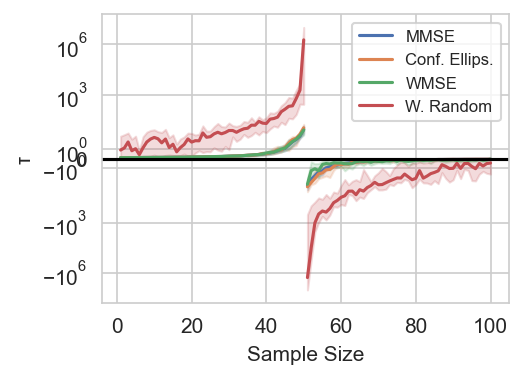
\includegraphics[width=\columnwidth]{figures/proj1/plots/LS_threshold/ER_0pt8_500_bandwidth_50_thresholds_LS.png}}
    \caption{Erdős–Rényi, 500 vertices} 
    \label{snr_ER}
    \end{subfigure}
    \hfill
    \begin{subfigure}{0.3\columnwidth}
    \resizebox{\width}{0.62\columnwidth}{
    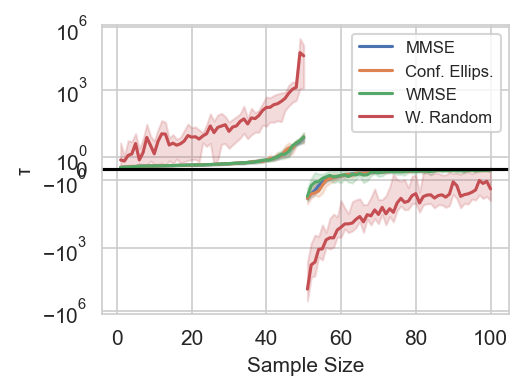
\includegraphics[width=\columnwidth]{figures/proj1/plots/LS_threshold/BA_3_500_bandwidth_50_thresholds_LS.png}}
    \caption{Barabási-Albert, 500 vertices}%
    \label{snr_BA}%
    \end{subfigure}
    \hfill%
    \begin{subfigure}{0.3\columnwidth}
    \resizebox{\width}{0.62\columnwidth}{
    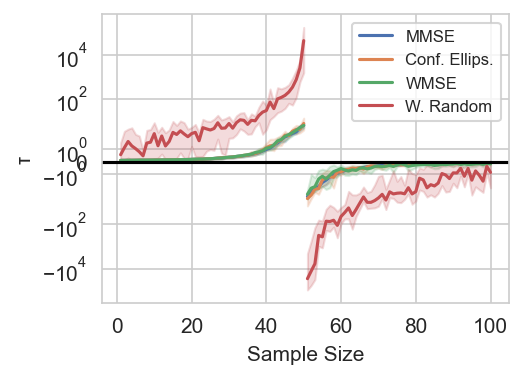
\includegraphics[width=\columnwidth]{figures/proj1/plots/LS_threshold/SBM_500_bandwidth_50_thresholds_LS.png}}
    \caption{SBM, 500 vertices}%
    \label{snr_SBM}%
    \end{subfigure}%
    \hfill
    \begin{subfigure}{0.3\columnwidth}
    \resizebox{\width}{0.62\columnwidth}{
    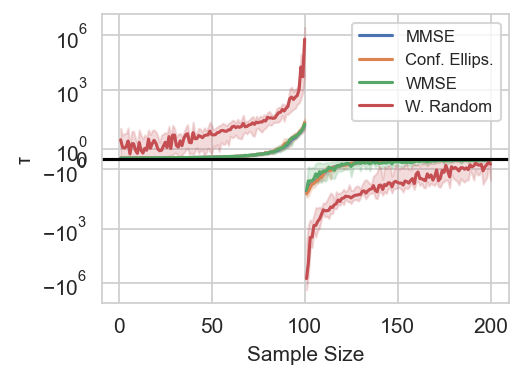
\includegraphics[width=\columnwidth]{figures/proj1/plots/LS_threshold/ER_0pt8_1000_bandwidth_100_thresholds_LS.png}}
    \caption{Erdős–Rényi, 1000 vertices} 
    \label{snr_ER_1000}
    \end{subfigure}
    \hfill
    \begin{subfigure}{0.3\columnwidth}
    \resizebox{\width}{0.62\columnwidth}{
    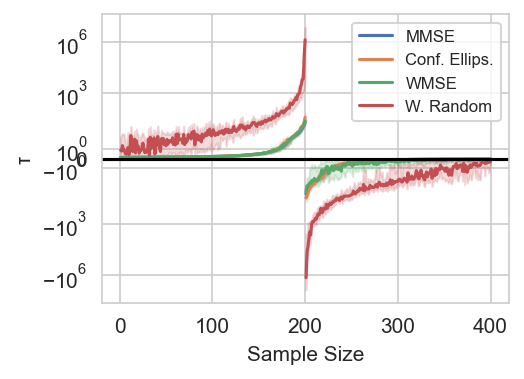
\includegraphics[width=\columnwidth]{figures/proj1/plots/LS_threshold/ER_0pt8_2000_bandwidth_200_thresholds_LS.png}}
    \caption{Erdős–Rényi, 2000 vertices}%
    \label{snr_ER_2000}%
    \end{subfigure}
    \hfill%
    \begin{subfigure}{0.3\columnwidth}
    \resizebox{\width}{0.62\columnwidth}{
    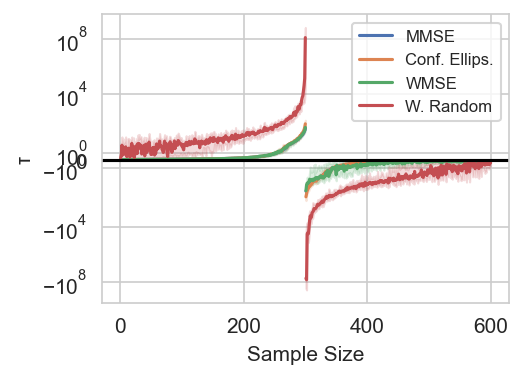
\includegraphics[width=\columnwidth]{figures/proj1/plots/LS_threshold/ER_0pt8_3000_bandwidth_300_thresholds_LS.png}}
    \caption{Erdős–Rényi, 3000 vertices}%
    \label{snr_ER_3000}%
    \end{subfigure}%
    \caption{$\tau(\set{S},v)$ for different random graph models and different $N$ under LS and full-band noise (bandwidth = $\frac{\# \text{ vertices}}{10}$)}
%\label{LS_SNR_Threshold_plots_big}
\label{LS_SNR_Threshold_plots_all}
\end{figure*}

%GLR_threshold_plots

\begin{figure*}%
    \centering
    \begin{subfigure}{0.3\columnwidth}
    \resizebox{\width}{0.62\columnwidth}{
    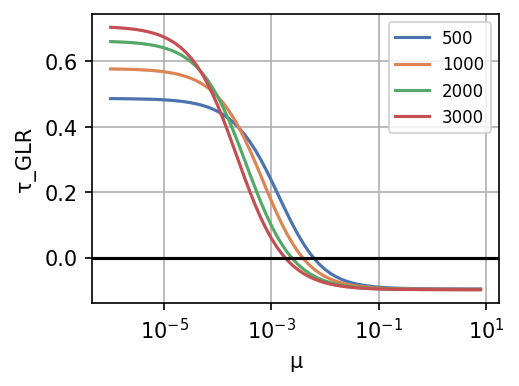
\includegraphics[width=\columnwidth]{figures/proj1/plots/GLR_threshold/ER_fb.png}}
    \caption{Erdős–Rényi ($\tau_{GLR}$)}
    \label{tau_GLR_er}
    \end{subfigure}
    \hfill
    \begin{subfigure}{0.3\columnwidth}
    \resizebox{\width}{0.62\columnwidth}{
    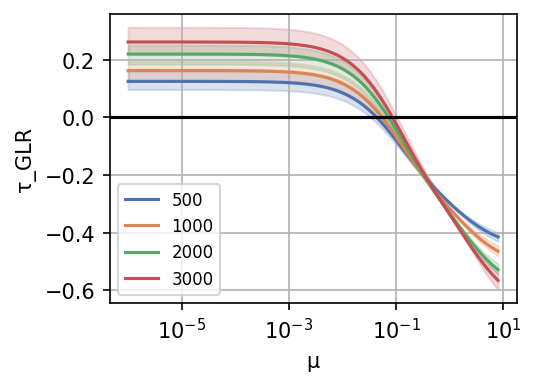
\includegraphics[width=\columnwidth]{figures/proj1/plots/GLR_threshold/BA_fb.png}}
    \caption{Barabási-Albert ($\tau_{GLR}$)}%
    \label{tau_GLR_BA}%
    \end{subfigure}
    \hfill%
    \begin{subfigure}{0.3\columnwidth}
    \resizebox{\width}{0.62\columnwidth}{
    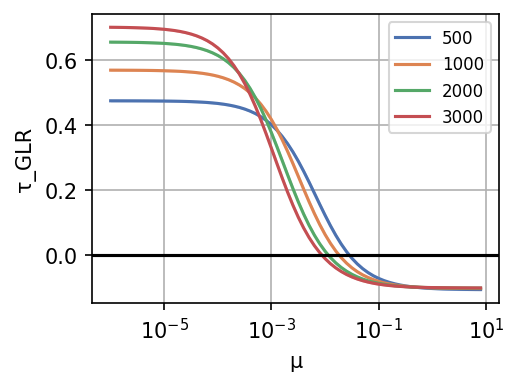
\includegraphics[width=\columnwidth]{figures/proj1/plots/GLR_threshold/SBM_fb.png}}
    \caption{SBM ($\tau_{GLR}$)}%
    \label{tau_GLR_SBM}%
    \end{subfigure}%
    \hfill
    \caption{$\tau_{GLR}$  for different random graph models (\#vertices = colour, bandwidth = $\frac{\text{\# vertices}}{10}$)}
\label{GLR_Threshold_plots}
\end{figure*}


%ER MSEs
\begin{figure*}%
    \centering
    \begin{subfigure}{0.3\columnwidth}
    \resizebox{\width}{0.62\columnwidth}{
    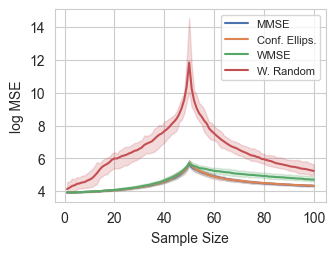
\includegraphics[width=\columnwidth]{figures/proj1/plots/LS_MSE/ER_0pt8_500_bandwidth_50_SNRdbs_-10.0_samps_100_MSE_LS.png}}
    \caption{Full-band noise, SNR = $10^{-1}$}
    \label{MSE_subfiga}
    \end{subfigure}\hfill
    \begin{subfigure}{0.3\columnwidth}
    \resizebox{\width}{0.62\columnwidth}{
    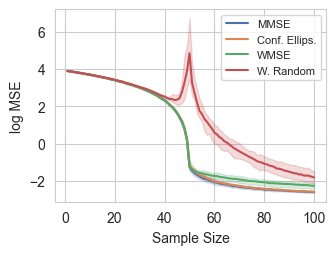
\includegraphics[width=\columnwidth]{figures/proj1/plots/LS_MSE/ER_0pt8_500_bandwidth_50_SNRdbs_20.0_samps_100_MSE_LS.png}}
    \caption{Full-band noise, SNR = $10^{2}$}%
    \label{MSE_subfigb}%
    \end{subfigure}\hfill%
    \begin{subfigure}{0.3\columnwidth}
    \resizebox{\width}{0.62\columnwidth}{
    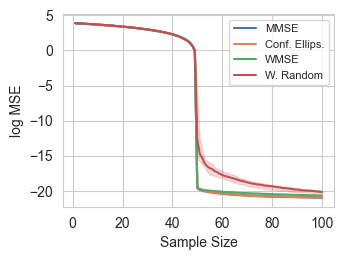
\includegraphics[width=\columnwidth]{figures/proj1/plots/LS_MSE/ER_0pt8_500_bandwidth_50_SNRdbs_100.0_samps_100_MSE_LS.png}}
    \caption{Full-band noise, SNR = $10^{10}$}%
    \label{MSE_subfigc}%
    \end{subfigure}%
    \caption{Average MSE under LS on ER Graphs (\#vertices=500, bandwidth = 50) }
\label{LS_ER_MSE_fig}
\end{figure*}



\begin{figure*}%
    \centering
    \begin{subfigure}{0.3\columnwidth}
    \resizebox{\width}{0.62\columnwidth}{
    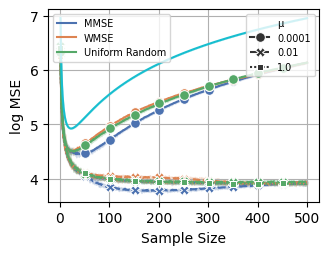
\includegraphics[width=\columnwidth]{figures/proj1/plots/GLR_MSE/ER_0pt8_500_bandwidth_50_SNRdbs_-10.0_samps_500_mus_0.0001_0.01_1_full_band.png}}
    \caption{Full-band noise, SNR = $10^{-1}$}
    \label{GLR_MSE_subfiga}
    \end{subfigure}\hfill
    \begin{subfigure}{0.3\columnwidth}
    \resizebox{\width}{0.62\columnwidth}{
    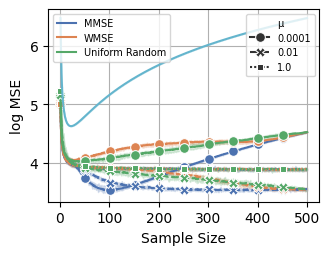
\includegraphics[width=\columnwidth]{figures/proj1/plots/GLR_MSE/ER_0pt8_500_bandwidth_50_SNRdbs_-3.01_samps_500_mus_0.0001_0.01_1_full_band.png}}
    \caption{Full-band noise, SNR = $\frac{1}{2}$}%
    \label{GLR_MSE_subfigb}%
    \end{subfigure}\hfill%
    \begin{subfigure}{0.3\columnwidth}
    \resizebox{\width}{0.62\columnwidth}{
    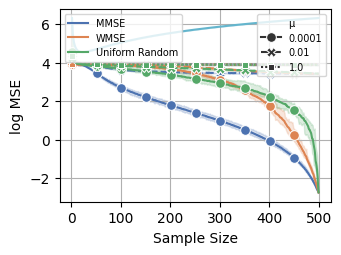
\includegraphics[width=\columnwidth]{figures/proj1/plots/GLR_MSE/ER_0pt8_500_bandwidth_50_SNRdbs_100.0_samps_500_mus_0.0001_0.01_1_full_band.png}}
    \caption{Full-band noise, SNR = $10^{10}$}%
    \label{GLR_MSE_subfigc}%
    \end{subfigure}%
    \caption{Average MSE under GLR on ER Graphs (\#vertices=500, bandwidth = 50), line without markers is an upper bound}
\label{GLR_ER_MSE_fig}
%\label{bandlimited_GLR_ER_MSE_fig}
\end{figure*}

%%% REAL DATASET experiments

\begin{figure}
    \centering
    \begin{subfigure}{0.3\columnwidth}
    %\resizebox{\width}{0.75\columnwidth}
    \resizebox{\width}{0.62\columnwidth}
    {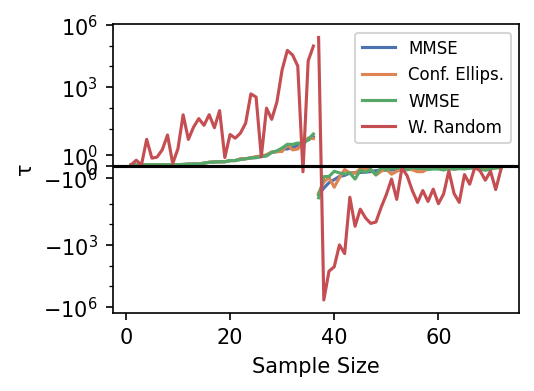
\includegraphics[width=\columnwidth]{figures/proj1/plots/LS_threshold_real/fmri_subsample_500_367_bandwidth_36_thresholds_LS.png}}
    \caption{FMRI} 
    \label{snr_FMRI}
    \end{subfigure}
    \begin{subfigure}{0.3\columnwidth}
    \resizebox{\width}{0.62\columnwidth}{
    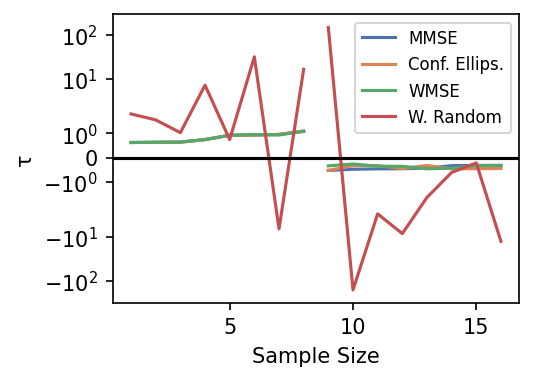
\includegraphics[width=\columnwidth]{figures/proj1/plots/LS_threshold_real/weather_45_bandwidth_8_thresholds_LS.png}}
    \caption{Weather}%
    \label{snr_Weather}%
    \end{subfigure}
    \caption{$\tau(\set{S},v)$ for real world datasets under LS and full-band noise}
\label{LS_SNR_Threshold_plots_all_real}
\end{figure}

\begin{figure}%
    \centering
    \begin{subfigure}{0.3\columnwidth}
    \resizebox{\width}{0.62\columnwidth}{
    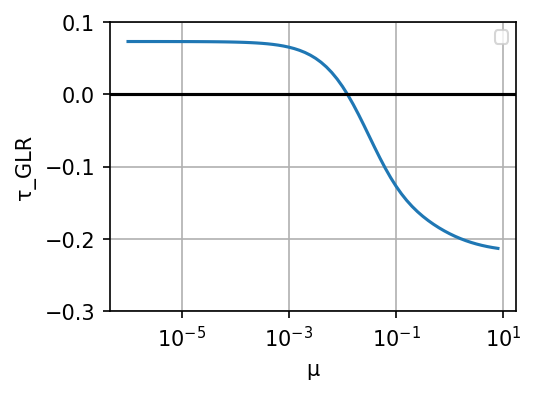
\includegraphics[width=\columnwidth]{figures/proj1/plots/GLR_threshold_real/fmri_subsample_500_GLR_threshold_fb.png}}
    \caption{FMRI}
    \label{tau_GLR_fmri}
    \end{subfigure}
    \begin{subfigure}{0.3\columnwidth}
    \resizebox{\width}{0.62\columnwidth}{
    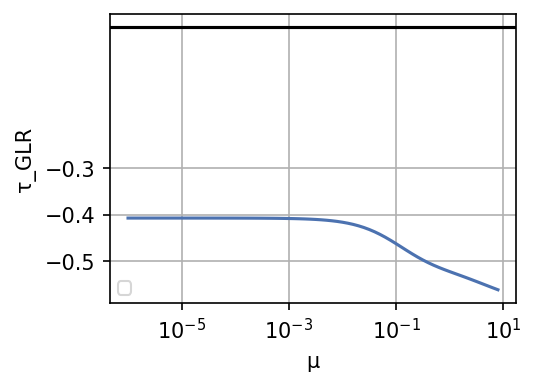
\includegraphics[width=\columnwidth]{figures/proj1/plots/GLR_threshold_real/weather_GLR_threshold_fb.png}}
    \caption{Weather}%
    \label{tau_GLR_weather}%
    \end{subfigure}
    \caption{$\tau_{GLR}$ for real world datasets}
\label{GLR_Threshold_plots_real}
\end{figure}


\begin{figure*}%
    \centering
    \begin{subfigure}{0.3\columnwidth}
    \resizebox{\width}{0.62\columnwidth}{
    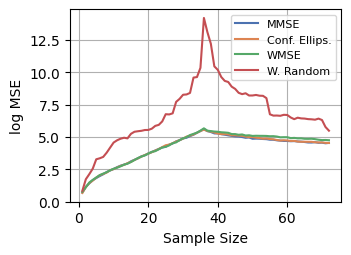
\includegraphics[width=\columnwidth]{figures/proj1/plots/LS_MSE_real/fmri_subsample_500_367_bandwidth_36_SNRdbs_-10.0_samps_72_fb_blsig_MSE_LS.png}}
    \caption{FMRI, SNR = $10^{-1}$}
    \label{fmri_MSE_subfiga}
    \end{subfigure}\hfill
    \begin{subfigure}{0.3\columnwidth}
    \resizebox{\width}{0.62\columnwidth}{
    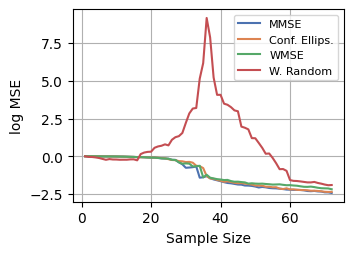
\includegraphics[width=\columnwidth]{figures/proj1/plots/LS_MSE_real/fmri_subsample_500_367_bandwidth_36_SNRdbs_20.0_samps_72_fb_blsig_MSE_LS.png}}
    \caption{FMRI, SNR = $10^{2}$}%
    \label{fmri_MSE_subfigb}%
    \end{subfigure}\hfill%
    \begin{subfigure}{0.3\columnwidth}
    \resizebox{\width}{0.62\columnwidth}{
    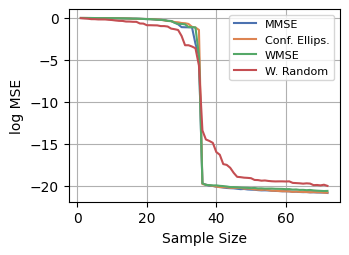
\includegraphics[width=\columnwidth]{figures/proj1/plots/LS_MSE_real/fmri_subsample_500_367_bandwidth_36_SNRdbs_100.0_samps_72_fb_blsig_MSE_LS.png}}
    \caption{FMRI, SNR = $10^{10}$}%
    \label{fmri_MSE_subfigc}%
    \end{subfigure}%
    \hfill
    \begin{subfigure}{0.3\columnwidth}
    \resizebox{\width}{0.62\columnwidth}{
    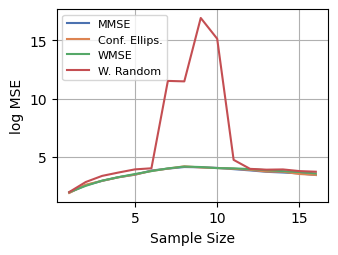
\includegraphics[width=\columnwidth]{figures/proj1/plots/LS_MSE_real/weather_45_bandwidth_8_SNRdbs_-10.0_samps_16_fb_blsig_MSE_LS.png}}
    \caption{Weather, SNR = $10^{-1}$}
    \label{weather_MSE_subfiga}
    \end{subfigure}\hfill
    \begin{subfigure}{0.3\columnwidth}
    \resizebox{\width}{0.62\columnwidth}{
    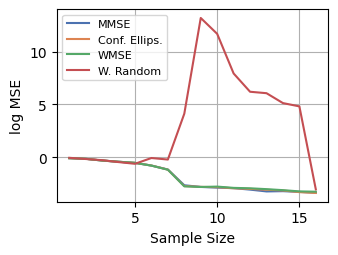
\includegraphics[width=\columnwidth]{figures/proj1/plots/LS_MSE_real/weather_45_bandwidth_8_SNRdbs_20.0_samps_16_fb_blsig_MSE_LS.png}}
    \caption{Weather, SNR = $1$}%
    \label{weather_MSE_subfigb}%
    \end{subfigure}\hfill%
    \begin{subfigure}{0.3\columnwidth}
    \resizebox{\width}{0.62\columnwidth}{
    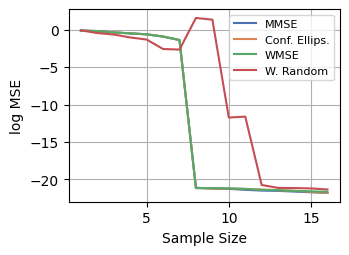
\includegraphics[width=\columnwidth]{figures/proj1/plots/LS_MSE_real/weather_45_bandwidth_8_SNRdbs_100.0_samps_16_fb_blsig_MSE_LS.png}}
    \caption{Weather, SNR = $10^{10}$}%
    \label{weather_MSE_subfigc}%
    \end{subfigure}%
    \caption{Average MSE under LS on real world datasets and full-band noise }
\label{LS_real_MSE_fig}
\end{figure*}

\begin{figure*}%
    \centering
    \begin{subfigure}{0.3\columnwidth}
    \resizebox{\width}{0.62\columnwidth}{
    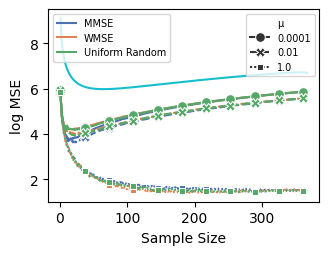
\includegraphics[width=\columnwidth]{figures/proj1/plots/GLR_MSE_real/fmri_subsample_500_367_bandwidth_36_SNRdbs_-10.0_samps_367_mus_0.0001_0.01_1_full_band_MSE_GLR.png}}
    \caption{FMRI, SNR = $10^{-1}$}
    \label{fmri_GLR_MSE_subfiga}
    \end{subfigure}\hfill
    \begin{subfigure}{0.3\columnwidth}
    \resizebox{\width}{0.62\columnwidth}{
    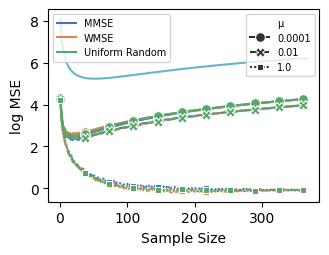
\includegraphics[width=\columnwidth]{figures/proj1/plots/GLR_MSE_real/fmri_subsample_500_367_bandwidth_36_SNRdbs_-3.010299956639812_samps_367_mus_0.0001_0.01_1_full_band_MSE_GLR.png}}
    \caption{FMRI, SNR = $\frac{1}{2}$}%
    \label{fmri_GLR_MSE_subfigb}%
    \end{subfigure}\hfill%
    \begin{subfigure}{0.3\columnwidth}
    \resizebox{\width}{0.62\columnwidth}{
    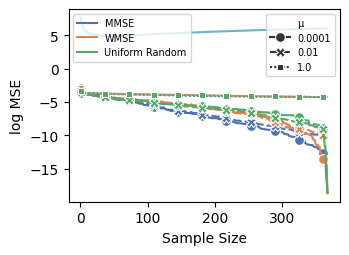
\includegraphics[width=\columnwidth]{figures/proj1/plots/GLR_MSE_real/fmri_subsample_500_367_bandwidth_36_SNRdbs_100.0_samps_367_mus_0.0001_0.01_1_full_band_MSE_GLR.png}}
    \caption{FMRI, SNR = $10^{10}$}%
    \label{fmri_GLR_MSE_subfigc}%
    \end{subfigure}%
    \hfill
    \begin{subfigure}{0.3\columnwidth}
    \resizebox{\width}{0.62\columnwidth}{
    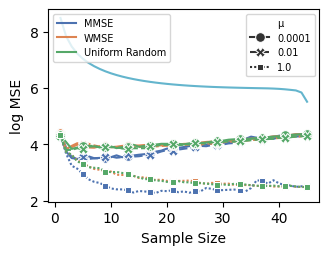
\includegraphics[width=\columnwidth]{figures/proj1/plots/GLR_MSE_real/weather_45_bandwidth_8_SNRdbs_-10.0_samps_45_mus_0.0001_0.01_1_full_band_MSE_GLR.png}}
    \caption{Weather, SNR = $10^{-2}$}
    \label{weather_GLR_MSE_subfiga}
    \end{subfigure}\hfill
    \begin{subfigure}{0.3\columnwidth}
    \resizebox{\width}{0.62\columnwidth}{
    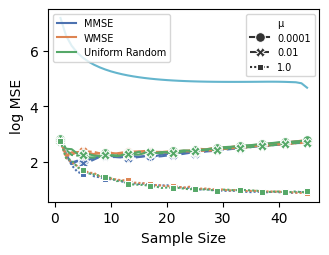
\includegraphics[width=\columnwidth]{figures/proj1/plots/GLR_MSE_real/weather_45_bandwidth_8_SNRdbs_-3.010299956639812_samps_45_mus_0.0001_0.01_1_full_band_MSE_GLR.png}}
    \caption{Weather, SNR = $\frac{1}{2}$}%
    \label{weather_GLR_MSE_subfigb}%
    \end{subfigure}\hfill%
    \begin{subfigure}{0.3\columnwidth}
    \resizebox{\width}{0.62\columnwidth}{
    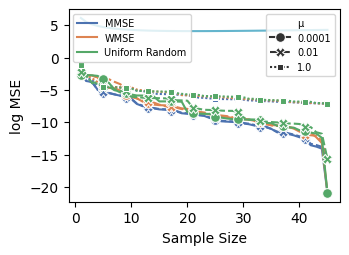
\includegraphics[width=\columnwidth]{figures/proj1/plots/GLR_MSE_real/weather_45_bandwidth_8_SNRdbs_100.0_samps_45_mus_0.0001_0.01_1_full_band_MSE_GLR.png}}
    \caption{Weather, SNR = $10^{10}$}%
    \label{weather_GLR_MSE_subfigc}%
    \end{subfigure}%
    \caption{Average MSE under GLR on real world datasets, line without markers is an upper bound}
\label{GLR_real_MSE_fig}
%\label{bandlimited_GLR_ER_MSE_fig}
\end{figure*}
\fi

Our theoretical results show how the relationship between sample size and MSE changes with the level of noise, focusing on how reducing sample size will reduce MSE if the SNR is below a threshold. In this section, we demonstrate  the applicability and validity of these results via empirical experiments. 

%Note that we always consider SNR in ratio form --- as $10^{x}$ rather than $\frac{x}{10} dB$ --- which is always positive. For the SNR to be below a given threshold (and so for us to show reducing sample size will decrease MSE) the threshold must be positive.

We first demonstrate the applicability of our results with plots of the thresholds $\tau(\set{S},v)$, $\tau_{GLR}$ and $\tau_{GLR\_bl}$ against sample size (Figs. \ref{LS_SNR_Threshold_plots_all} and \ref{GLR_Threshold_plots}). These plots show concrete SNR values for the thresholds, giving a practical understanding of how high noise levels need to be for reducing sample size to reduce MSE for different random graph models and parameters. Additionally, we empirically tabulate the probabilities that graphs from each model  satisfy the conditions of our theorems (Table \ref{tbl:empirical_probabilities_conditions}), allowing the reader to evaluate the impact of our theorems across different applications. We then demonstrate the validity of our results by plotting $\textrm{MSE}_{\set{S}}$ against sample size (Figs. \ref{LS_ER_MSE_fig} and  \ref{GLR_ER_MSE_fig}) at SNRs below, near and above the derived thresholds, showing that the behaviour of $\textrm{MSE}_{\set{S}}$ follows our theoretical results. \bs{We finally present similar results on real-world datasets, validating the applicability of our results to real world datasets.}

\subsection{Experimental Setup}
We now present the setup of the experiments. All results are presented with 90\% confidence intervals and all experiments use the combinatorial Laplacian $\matr{L}$ and its eigenbasis.
\subsubsection{\bs{Synthetic} Graph Generation}
We consider each of the following unweighted random graph models:
\begin{itemize}
    \item Erdős–Rényi (ER) with edge probability $p=0.8$ (experiments with other values of $p$ show similar results)
    \item Barabási-Albert (BA) with a preferential attachment to 3 vertices at each step of its construction
    \item Stochastic Blockmodel (SBM) with intra- and inter-cluster edge probabilities of $0.7 \text{ and }0.1$ respectively
    %\item Ring (Ring).
\end{itemize}
We consider 10 instantiations of each model for plots, and 1000 instantiations of each model to assess the probability the graph invariant conditions in our Theorems are met.

We present threshold plots for graphs with 500, 1000, 2000 and 3000 vertices. We only present MSE plots for graphs with 500 vertices  {\color{black}  (like \cite[Fig 8]{bai2020fast})} as they are intended as an accompaniment to our threshold plots and theorems to demonstrate their validity, and a single graph size suffices. 

\subsubsection{\xd{Synthetic} Signal Generation}
We set the bandwidth  $k = \lfloor \frac{N}{10} \rfloor$, as per \cite{bai2020fast}.  We consider the following SNRs:

\begin{itemize}
    \item{\makebox[8em][l]{Full-band noise:}  $10^{-1}, 10^{2}, 10^{10}$ (i.e. $-10dB, 20dB, 100dB$)}
    \item{\makebox[8em][l]{Bandlimited noise:}  $10^{-1}, 1, 10^{10}$ (i.e. $-10dB, 0dB, 100dB$)}
\end{itemize}
These SNRs are chosen to demonstrate that there are three regimes for MSE with distinctive properties---the high noise regime, the transitionary regime and the approximately noiseless regime---and that $\tau$ captures when the regimes change. Suitable values of SNRs to demonstrate this vary between reconstruction methods and noise types, hence our choices.
%Note that we always consider SNR in ratio form---as $10^{x}$ rather than $\frac{x}{10} dB$---which is always positive. For the SNR to be below a given threshold (and so for us to show reducing sample size will decrease MSE) the threshold must be positive.

To test the MSE in reconstructing signals from samples \bs{on random graph models}, we generate 200 signals by sampling $\vect{y} = \vect{x}_{raw} + \sigma \cdot \epsilon_{raw}$ where:
\begin{enumerate}
    \item $\vect{x}_{raw} \sim \mathcal{N}(\vect{0}, \matr{\Pi}_{bl(\set{K})})$ 
    \item[2a)] If full-band noise, $\vect{\epsilon}_{raw} \sim \mathcal{N}(\vect{0}, \matr{I}_{N})$, $\sigma = \sqrt{\frac{k}{{N \cdot\text{SNR}}}}$
    \item[2b)]  If bandlimited noise, $\vect{\epsilon}_{raw} \sim \mathcal{N}(\vect{0}, \projbl )$, $\sigma = \frac{1}{\sqrt{\text{SNR}}}$ 
    %\item Normalise $\vect{x}_{raw}$ and $\vect{\epsilon}_{raw}$ to have norm 1
    %\item Normalise: $\vect{x} = \frac{\vect{x}_{raw}}{||\vect{x}_{raw}||_{2}}$ and $\vect{\epsilon} = \frac{\vect{\epsilon}_{raw}}{ ||\vect{\epsilon}_{raw}||_{2}}$
    %\item[3)] Return $\vect{y} = \vect{x} + \frac{\vect{\epsilon}}{\sqrt{\text{SNR}}}$
    %\item[3)] Return $\vect{y} = \vect{x} + \sigma \cdot \epsilon$
\end{enumerate}
%For the cases of bandlimited noise, in step (1) we generate $\vect{\epsilon}_{raw} \sim \mathcal{N}(\vect{0}, \projbl )$ instead.

\subsubsection{Real World Datasets}
\bs{
We also consider two real world datasets as in \cite{zhi2023gaussian}. The first is an FMRI dataset, where the original graph consists of 4465 nodes corresponding to voxels of the cerebellum, with 292 Blood-Oxygen-Level-Dependent (BOLD) signals derived from FMRI. We sample a connected subgraph of 367 nodes via Neighbourhood Sampling \cite{hamilton2017inductive}. The second is a Weather dataset, where a $10$-nearest neighbours graph of 45 cities in Sweden is constructed, with 95 signals derived from the temperature. See \cite{venkitaraman2020gaussian, behjat2016signal, zhi2023gaussian} for details on graph construction and signal generation in both cases. 
We generate $\vect{x}$ by $k$-bandlimiting the original signals, where For FMRI we set $k=36$ and for Weather dataset we set $k=8$. We otherwise follow the above methodology in Synthetic Signal Generation for generating signals with full-band noise.
}


\subsubsection{Sample-Set Selection}
%The literature provides several approximations to make vertex sample-set selection efficient; for example, approximating the projection matrix $\projbl$ \cite{wang2018optimal} (subsets of which are used to compute optimality criteria) with a polynomial in $\matr{L}$, and approximating optimality criteria for easier computation \cite{bai2020fast}. 

We generate sample sets greedily using exact analytic forms and by exactly computing $\matr{\Pi}_{bl(\set{K})}$.
\begin{itemize}
    \item[LS:] We use (\ref{eq:A-optimality})-(\ref{eq:E-optimality}) to exactly compute the MMSE {\color{black}\cite{wang2018optimal,wang2019low, mfn}}, Confidence Ellipsoid {\color{black}\cite{jayawant2021doptimal, tremblay2017determinantal,mfn}} and WMSE criteria {\color{black} \cite{bai2020fast}}, which are deterministic and guaranteed to be noiseless-optimal.  We also look at Weighted Random sampling \cite{puy2018random}, which is neither deterministic nor guaranteed to be noiseless-optimal.
\end{itemize}
Note that sampling schemes in the literature tend to differ from ours mainly in that they approximate our setup for computational efficiency reasons; e.g. approximating the projection matrix $\projbl$ with a polynomial in $\matr{L}$ \cite{wang2018optimal}, and approximating optimality criteria \cite{bai2020fast}. As these differences are for efficiency reasons, we do not expect them to matter in our experiments.

\subsubsection{Parameters of Reconstruction Methods} We consider LS with the previously stated bandwidth.

\subsection{Experimental Results --- Synthetic Graphs}

\begin{figure*}
    \centering
    \begin{subfigure}{0.3\columnwidth}
    %\resizebox{\width}{0.75\columnwidth}
    \resizebox{\width}{0.62\columnwidth}
    {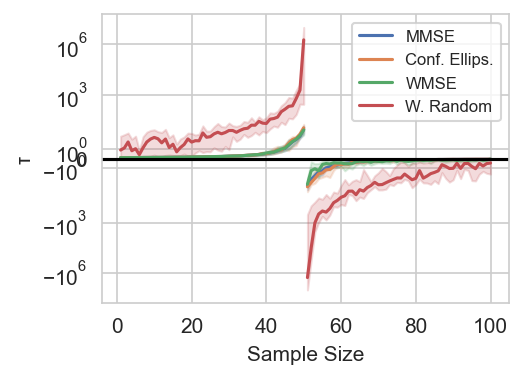
\includegraphics[width=\columnwidth]{figures/proj1/plots/LS_threshold/ER_0pt8_500_bandwidth_50_thresholds_LS.png}}
    \caption{Erdős–Rényi, 500 vertices} 
    \label{snr_ER}
    \end{subfigure}
    \hfill
    \begin{subfigure}{0.3\columnwidth}
    \resizebox{\width}{0.62\columnwidth}{
    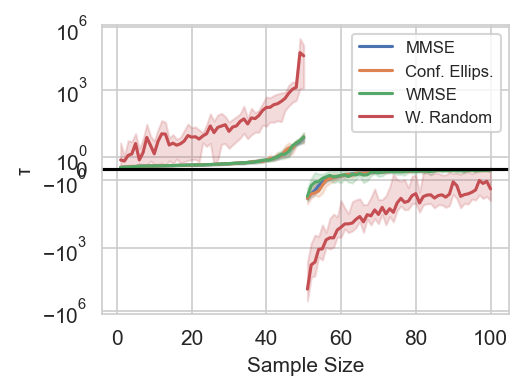
\includegraphics[width=\columnwidth]{figures/proj1/plots/LS_threshold/BA_3_500_bandwidth_50_thresholds_LS.png}}
    \caption{Barabási-Albert, 500 vertices}%
    \label{snr_BA}%
    \end{subfigure}
    \hfill%
    \begin{subfigure}{0.3\columnwidth}
    \resizebox{\width}{0.62\columnwidth}{
    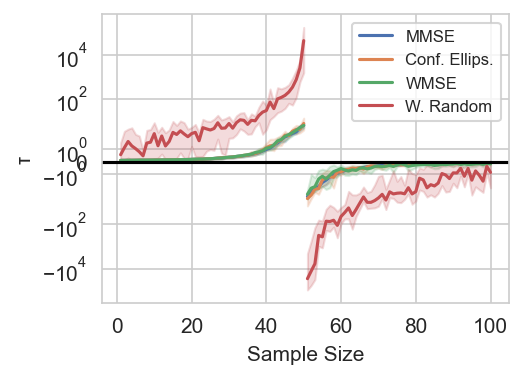
\includegraphics[width=\columnwidth]{figures/proj1/plots/LS_threshold/SBM_500_bandwidth_50_thresholds_LS.png}}
    \caption{SBM, 500 vertices}%
    \label{snr_SBM}%
    \end{subfigure}%
    \hfill
    \begin{subfigure}{0.3\columnwidth}
    \resizebox{\width}{0.62\columnwidth}{
    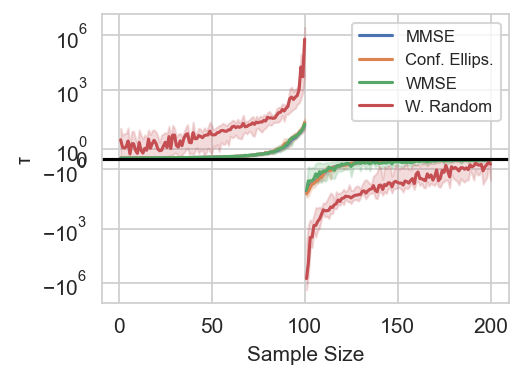
\includegraphics[width=\columnwidth]{figures/proj1/plots/LS_threshold/ER_0pt8_1000_bandwidth_100_thresholds_LS.png}}
    \caption{Erdős–Rényi, 1000 vertices} 
    \label{snr_ER_1000}
    \end{subfigure}
    \hfill
    \begin{subfigure}{0.3\columnwidth}
    \resizebox{\width}{0.62\columnwidth}{
    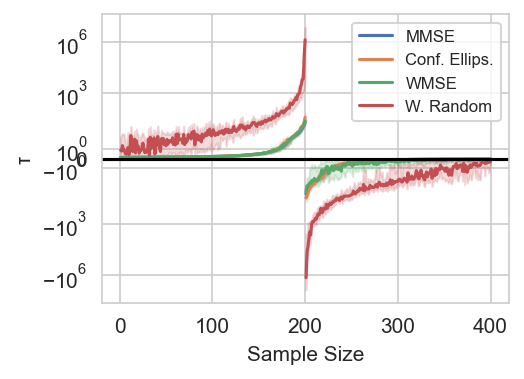
\includegraphics[width=\columnwidth]{figures/proj1/plots/LS_threshold/ER_0pt8_2000_bandwidth_200_thresholds_LS.png}}
    \caption{Erdős–Rényi, 2000 vertices}%
    \label{snr_ER_2000}%
    \end{subfigure}
    \hfill%
    \begin{subfigure}{0.3\columnwidth}
    \resizebox{\width}{0.62\columnwidth}{
    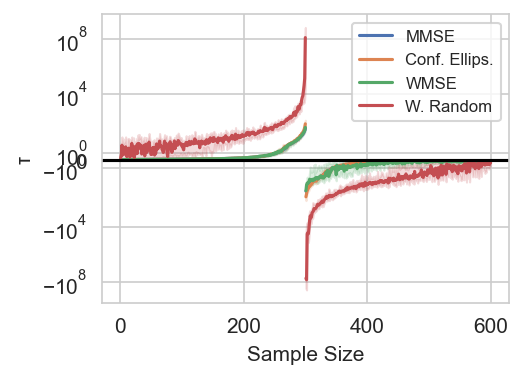
\includegraphics[width=\columnwidth]{figures/proj1/plots/LS_threshold/ER_0pt8_3000_bandwidth_300_thresholds_LS.png}}
    \caption{Erdős–Rényi, 3000 vertices}%
    \label{snr_ER_3000}%
    \end{subfigure}%
    \caption{$\tau(\set{S},v)$ for different random graph models and different $N$ under LS and full-band noise (bandwidth = $\frac{\# \text{ vertices}}{10}$)}
%\label{LS_SNR_Threshold_plots_big}
\label{LS_SNR_Threshold_plots_all}
\end{figure*}

%GLR_threshold_plots

\begin{figure*}%
    \centering
    \begin{subfigure}{0.3\columnwidth}
    \resizebox{\width}{0.62\columnwidth}{
    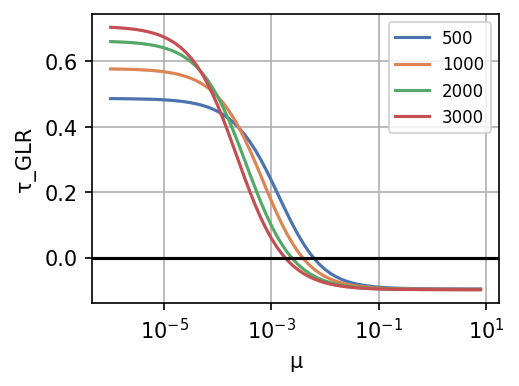
\includegraphics[width=\columnwidth]{figures/proj1/plots/GLR_threshold/ER_fb.png}}
    \caption{Erdős–Rényi ($\tau_{GLR}$)}
    \label{tau_GLR_er}
    \end{subfigure}
    \hfill
    \begin{subfigure}{0.3\columnwidth}
    \resizebox{\width}{0.62\columnwidth}{
    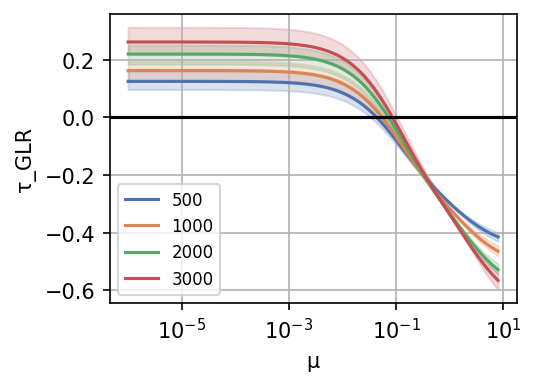
\includegraphics[width=\columnwidth]{figures/proj1/plots/GLR_threshold/BA_fb.png}}
    \caption{Barabási-Albert($\tau_{GLR}$)}%
    \label{tau_GLR_BA}%
    \end{subfigure}
    \hfill%
    \begin{subfigure}{0.3\columnwidth}
    \resizebox{\width}{0.62\columnwidth}{
    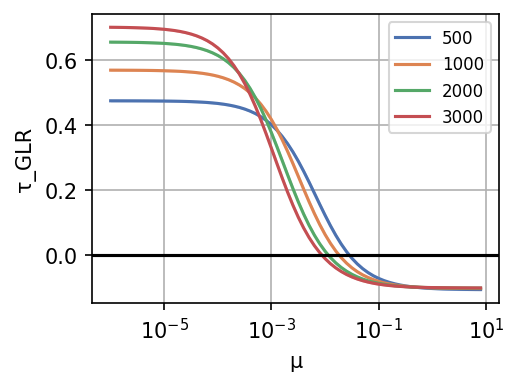
\includegraphics[width=\columnwidth]{figures/proj1/plots/GLR_threshold/SBM_fb.png}}
    \caption{SBM ($\tau_{GLR}$)}%
    \label{tau_GLR_SBM}%
    \end{subfigure}%
    \hfill
    \caption{$\tau_{GLR}$  for different random graph models (\#vertices = colour, bandwidth = $\frac{\text{\# vertices}}{10}$)}
\label{GLR_Threshold_plots}
\end{figure*}


%ER MSEs
\begin{figure*}%
    \centering
    \begin{subfigure}{0.3\columnwidth}
    \resizebox{\width}{0.62\columnwidth}{
    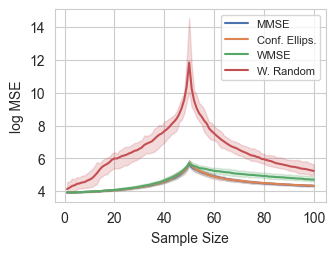
\includegraphics[width=\columnwidth]{figures/proj1/plots/LS_MSE/ER_0pt8_500_bandwidth_50_SNRdbs_-10.0_samps_100_MSE_LS.png}}
    \caption{Full-band noise, SNR = $10^{-1}$}
    \label{MSE_subfiga}
    \end{subfigure}\hfill
    \begin{subfigure}{0.3\columnwidth}
    \resizebox{\width}{0.62\columnwidth}{
    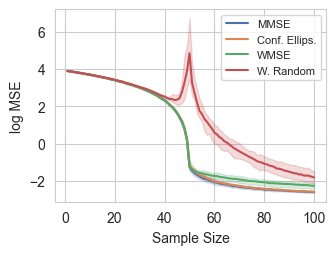
\includegraphics[width=\columnwidth]{figures/proj1/plots/LS_MSE/ER_0pt8_500_bandwidth_50_SNRdbs_20.0_samps_100_MSE_LS.png}}
    \caption{Full-band noise, SNR = $10^{2}$}%
    \label{MSE_subfigb}%
    \end{subfigure}\hfill%
    \begin{subfigure}{0.3\columnwidth}
    \resizebox{\width}{0.62\columnwidth}{
    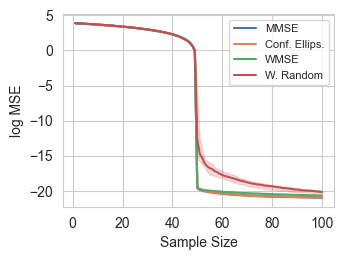
\includegraphics[width=\columnwidth]{figures/proj1/plots/LS_MSE/ER_0pt8_500_bandwidth_50_SNRdbs_100.0_samps_100_MSE_LS.png}}
    \caption{Full-band noise, SNR = $10^{10}$}%
    \label{MSE_subfigc}%
    \end{subfigure}%
    \caption{Average MSE under LS on ER Graphs (\#vertices=500, bandwidth = 50) }
\label{LS_ER_MSE_fig}
\end{figure*}





For full-band noise, we present threshold plots for all graphs and MSE plots for ER graphs in the main body of the paper. MSE plots for BA and SBM graphs are presented in Appendix \ref{plot_appendix}. For bandlimited noise, we present threshold plots, MSE plots and discussion of how the experimental and theoretical results correspond in Appendix \ref{app:Experiments_Bandlimited}.
{\color{black} We also present Table \ref{tbl:theory_experiment_correspondence} showing how our plots correspond to our theoretical results, which also corresponds to the summary of theoretical results in Table \ref{tbl:general_theory}.}

\iffalse
\begin{table}[h]
{\color{black}
\caption{Correspondence of Theory and Empirical Results}
\centering
\begin{tabularx}{(\textwidth)}{|X|p{2.6cm}|p{2.5cm}|p{2.6cm}|p{2.6cm}|}%{|@{\hspace{0.1cm}}p{2.6cm}|p{2.6cm}|p{2.6cm}|p{2.6cm}|X|}
\hline
\multirow{2}{*}{} & \multicolumn{2}{c|}{\textbf{LS}} & \multicolumn{2}{c|}{\textbf{GLR}} \\
\cline{2-5}
 & Full-band & Bandlimited & Full-band & Bandlimited \\
\hline
\textbf{Character- isation} & 
\makecell{Corr \ref{main_ls} \\
(Figs. \ref{snr_ER}-\ref{snr_SBM}\\
\& \ref{MSE_subfiga}-\ref{MSE_subfigc})} & 
\makecell{Corr \ref{corr:LS_bandlimited_noise_big_variance} \\ (Figs. \ref{bandlimited_MSE_subfiga}-\\ \ref{bandlimited_MSE_subfigc})} & 
\multicolumn{2}{c|}{\makecell{Corr \ref{corr:main_GLR_iff} \\ (Figs. \ref{GLR_MSE_subfiga}-\ref{GLR_MSE_subfigc})}
} \\
\hline
\textbf{Existence} & 
\makecell{Thm \ref{thm:noiseless_optimality_means_noise_sensitivity} \\ (Figs. \ref{snr_ER}-\ref{snr_SBM}\\
\& \ref{MSE_subfiga}-\ref{MSE_subfigc})} & 
\makecell{Corr \ref{corr:LS_bandlimited_noise_sample_only_k} \\ (Figs. \ref{bandlimited_MSE_subfiga}- \\ \ref{bandlimited_MSE_subfigc})} & 
\makecell{Thm \ref{thm:main_GLR_exist} \\
 (Figs. \ref{tau_GLR_er}-\ref{tau_GLR_SBM} \\ \& \ref{GLR_MSE_subfiga}-\ref{GLR_MSE_subfigc}\\
 \& Table \ref{tbl:empirical_probabilities_conditions})
} & 
\makecell{Thm \ref{thm:main_GLR_bl} \\
(Figs. \ref{tau_GLR_bl_er}-\ref{tau_GLR_bl_SBM} \\ \& \ref{bandlimited_GLR_MSE_subfiga}-\ref{bandlimited_GLR_MSE_subfigc} \\
\& Table \ref{tbl:empirical_probabilities_conditions_bl})
} \\
\hline
\textbf{Asymptotics} & 
\makecell{Rmk \ref{rmk:LS_big_N} \\ (Figs. \ref{snr_ER_1000}-\ref{snr_ER_3000})} & 
\makecell{\\ Rmk \ref{rmk:LS_big_N_bl}} & 
\makecell{Propn \ref{propn:GLR_big_N} \\ (Figs. \ref{tau_GLR_er}-\ref{tau_GLR_SBM})} & 
\makecell{Propn \ref{propn:GLR_big_N_bl} \\ (Figs. \ref{tau_GLR_bl_er}-\ref{tau_GLR_bl_SBM})} \\
\hline
\end{tabularx}
\label{tbl:theory_experiment_correspondence}
}
\end{table}
\fi

% Table 1: LS columns only
\begin{table}[h]
\caption{Correspondence of Theory and Empirical Results - LS}
\centering
\begin{tabularx}{\textwidth}{l >{\centering\arraybackslash}p{15em} >{\centering\arraybackslash}X}
\toprule
& \multicolumn{2}{c}{\textbf{LS}} \\
\cmidrule(lr){2-3}
 & Full-band Noise & Bandlimited Noise \\
\midrule
\textbf{Characterisation} & 
\makecell[c]{Corr \ref{main_ls} \\
(Figs. \ref{snr_ER}-\ref{snr_SBM} 
\& \ref{MSE_subfiga}-\ref{MSE_subfigc})} & 
\makecell[c]{Corr \ref{corr:LS_bandlimited_noise_big_variance} \\ (Figs. \ref{bandlimited_MSE_subfiga}- \ref{bandlimited_MSE_subfigc})} \\
\midrule
\textbf{Existence} & 
\makecell[c]{Thm \ref{thm:noiseless_optimality_means_noise_sensitivity} \\ (Figs. \ref{snr_ER}-\ref{snr_SBM}
\& \ref{MSE_subfiga}-\ref{MSE_subfigc})} & 
\makecell[c]{Corr \ref{corr:LS_bandlimited_noise_sample_only_k} \\ (Figs. \ref{bandlimited_MSE_subfiga}- \ref{bandlimited_MSE_subfigc})} \\
\midrule
\textbf{Asymptotics} & 
\makecell[c]{Rmk \ref{rmk:LS_big_N} \\ (Figs. \ref{snr_ER_1000}-\ref{snr_ER_3000})} & 
\makecell[c]{Rmk \ref{rmk:LS_big_N_bl}\\} \\
\bottomrule
\end{tabularx}
\label{tbl:theory_experiment_correspondence_LS}
\end{table}



%\subsubsection{\texorpdfstring{$\tau$ and $\tau_{GLR}$ plots}{\texttau and \texttau\_GLR plots}}
\subsubsection{$\tau$ plots (LS)}

%Our threshold plots demonstrate the applicability of our theorems. We remember that SNR is in ratio form (not in $dB$) and so always positive by definition. We overlay a black line at $\tau = 0$ to emphasise how when $\tau > 0$ and $0 < \textrm{SNR} < \tau$, we have proven that reducing sample size can reduce MSE. 

%As the thresholds are bounds on the ratio form of SNR (not in $dB$), we overlay a black line at 0. This is meaningful because our theorems only say 
%Our threshold plots demonstrate the applicability of our theorems. Our threshold plots are bounds on the ratio form of SNR (not in $dB$), so the transition between negative and positive is important; therefore, we overlay a black line at 0.
%\,\\
%\emph{[LS]:} 
Figs. \ref{LS_SNR_Threshold_plots_all}  shows $\tau(\set{S},v)$ as sample size varies for sequential sampling methods under LS, where $v$ is the latest node added to $\set{S}$. 
 % We interpret the subfigures of Fig. \ref{LS_SNR_Threshold_plots}:
 % \begin{itemize}
     % \item[(a)] 
     For ER graphs, for sample size smaller than the bandwidth, $\tau(\set{S},v) > 0$ and beyond that $\tau(\set{S},v) \leq 0$. The maximum of $\tau(\set{S},v)$ observed is approximately $10^{6}$ ($60dB$) for weighted random sampling, and approximately 10 ($10dB$) for the deterministic sampling methods. The confidence intervals for weighted random sampling is much wider than for the deterministic sampling methods.
     Next, we observe the same phenomenon as with ER for BA and SBM graphs, with maxima of approximately $10^5$ ($50dB$) for weighted random sampling and maxima of approximately 10 ($10dB$) for the deterministic sampling methods.
% \end{itemize}
Finally, Figs. \ref{snr_ER_1000}-\ref{snr_ER_3000} show the same phenomenon as Fig. \ref{snr_ER} happens for ER graphs at sizes of 1000, 2000 and 3000 vertices.

 We now correlate our experiments and our theoretical results. As Corollary \ref{main_ls} is necessary and sufficient, the sign of $\tau(\set{S},v)$ tells us exactly when removing a vertex improves $\set{S}$. Therefore $\tau$ being negative is an informative statement, telling us that $\set{S} \backslash \{v\}$ is \emph{never} better than $\set{S}$. Concretely, if SNR is below the maximum $\tau(\set{S},v)$ observed, then when sample size equals bandwidth we can reduce sample size to reduce MSE.

 Theorem \ref{thm:noiseless_optimality_means_noise_sensitivity} proves that noiseless-optimal methods (MMSE, Confidence Ellipsoid and WMSE in our experiments) will have $\tau(\set{S},v) > 0$ for sample sizes smaller than the bandwidth, and then $\tau(\set{S},v) \leq 0$ afterwards, and Fig. \ref{LS_SNR_Threshold_plots_all}  validates this. Note that even though this pattern holds for Weighted Random Sampling in our experiments, Theorem \ref{thm:noiseless_optimality_means_noise_sensitivity} does not guarantee it always holds for Weighted Random Sampling.

 While we prove that $\tau(\set{S},v) \not\to 0$ as $N \to \infty$, we conjecture the stronger claim that at a sample size equal to bandwidth, $\tau(\set{S},v)$ might actually increase with graph size, which is supported (but not proven) by Figs. \ref{snr_ER_1000}-\ref{snr_ER_3000}.
 %We need $\textrm{SNR} > 10^{6}$ ($60dB$) for removing samples to not decrease MSE. %Comparing to the threshold plots for smaller $N$ (see Appendix \ref{plot_appendix}, Fig. \ref{fig:LS_SNR_Threshold_plots_small}) to Fig. \ref{LS_SNR_Threshold_plots} suggests that the thresholds get larger with $N$ --- a wider range of SNRs exhibit the phenomenon of reducing sample size reducing MSE on larger graphs.

\subsubsection{MSE plots (LS)}
The MSE plots demonstrate the validity of our theoretical results linking MSE and sample size.

%\emph{[LS]:} 
Figs. \ref{MSE_subfiga}-\ref{MSE_subfigc} show log MSE against sample size for LS under full-band noise. %We interpret its subfigures:
% \begin{itemize}
    % \item[(a)] 
    For high noise (a), we see MSE increases with sample size no larger than bandwidth, and decreases afterwards -- \bs{that is, it is $\Lambda$-shaped, as described in Remark \ref{remark:LS_error_lambda_shaped}}. %with sample size when sample size $\geq$ bandwidth.
    In (b), for our three deterministic noiseless-optimal sampling schemes (orange/green/blue), MSE is decreasing in sample size. For weighted random sampling, we see for sample sizes no larger than bandwidth, MSE first decreases and then increases, attaining a maximum with sample size at bandwidth, and then decreases with sample size.
    In (c), the almost noiseless case, we see MSE is decreasing in sample size for all sampling schemes, with a large drop when sample size is at bandwidth.
% \end{itemize}

Comparing Figs. \ref{MSE_subfiga}-\ref{MSE_subfigc} to Fig. \ref{snr_ER}, Fig. \ref{MSE_subfiga} corresponds to when $\text{SNR} < \tau(\set{S},v)$, Fig. \ref{MSE_subfigc} corresponds to $\text{SNR} > \tau(\set{S},v)$ and Fig. \ref{MSE_subfigb} corresponds to when SNR lies between some values of $\tau(\set{S},v)$ for weighted random sampling.  
We see that MSE increases with sample size when $\text{SNR} < \tau(\set{S},v)$ and decreases otherwise, proving the validity of Corollary \ref{main_ls}.
Fig. \ref{MSE_subfiga} (green, orange, blue curves) shows that for low SNRs, optimal sampling schemes  lead MSE to monotonically increase with each additional sample until the sample size reaches the bandwidth, illustrating Theorem \ref{thm:noiseless_optimality_means_noise_sensitivity} and Remark \ref{remark:LS_error_lambda_shaped}. We also validate Remark \ref{remark:remove_multiple_nodes}: if we are slightly above the bandwidth ($50$ for Fig. \ref{MSE_subfiga}), i.e., to the right of the peak, then reducing sample size by one does not reduce MSE; however, if we significantly reduce sample size, i.e., transitioning from just right of the peak to left of the peak, we can reduce MSE. %We provide further discussion of the $\Lambda$-shape of the MSE below Remark \ref{remark:LS_error_lambda_shaped}.

%Comparing Fig. \ref{MSE_subfiga} and \ref{MSE_subfigc} shows that for low SNRs, MSE can increase with sample size (Fig. \ref{MSE_subfiga}), 

Interestingly, Fig. \ref{MSE_subfiga} shows that at a low SNR of $10^{-1}$, the optimal sample size under LS is zero. Although this might appear counter-intuitive at a first glance, it makes concrete the idea that reconstruction does not work if there is too much noise: at this noise level letting $\vect{\hat{x}} = \vect{0}$ rather than fitting with LS with any number of observed vertices will result in a lower MSE on average. We can also formalise this in terms of our Bias-Variance decomposition; a $\vect{0}$ reconstruction has high bias but zero variance, and reconstructing from a non-zero number of samples has lower bias but positive variance. At a high enough noise the variance term in the MSE will dominate, and the MSE from taking $\hat{\vect{x}} = \vect{0}$ will be lower than reconstructing from any non-zero number of samples. The same reasoning applies to why the MSE at a smaller number of samples (e.g. 5 samples) is better than a larger number (e.g. 100 samples).

%One interpretation of this observation is that, under very high noise, if you throw away all of your samples and assume that your underlying signal is $\vect{0}$, you will on average have a lower MSE than if you reconstruct with LS from your observed samples. This follows from (\ref{eq:xi_decomp}) and the positivity of $\xi_{1}$ and $\xi_{2}$ --- if your error increases unboundedly with noise, at a sufficiently high noise level your MSE will be above the fixed MSE you would get by approximating your signal with $\vect{0}$.

On the other hand, for high SNRs (Fig. \ref{MSE_subfigc}), MSE decreases monotonically as sample size increases for all sampling schemes, showing Corollary \ref{main_ls} is necessary and sufficient. %Fig. \ref{MSE_subfigb} shows an intermediate case: for SNRs between these extremes some schemes (Red line) lead to increasing MSE with increasing sample size, while other schemes (Blue, Green, Orange lines) do not.
Finally, Fig. \ref{MSE_subfigb} illustrates the situation between the two cases.

{\color{black}
\subsection{Experimental Results --- Real World Datasets}

%%% REAL DATASET experiments

\begin{figure}
    \centering
    \begin{subfigure}{0.31\columnwidth}
    %\resizebox{\width}{0.75\columnwidth}
    \resizebox{\width}{0.62\columnwidth}
    {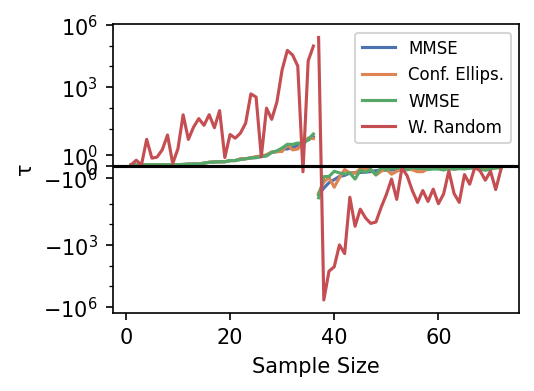
\includegraphics[width=\columnwidth]{figures/proj1/plots/LS_threshold_real/fmri_subsample_500_367_bandwidth_36_thresholds_LS.png}}
    \caption{FMRI} 
    \label{snr_FMRI}
    \end{subfigure}
    \begin{subfigure}{0.31\columnwidth}
    \resizebox{\width}{0.62\columnwidth}{
    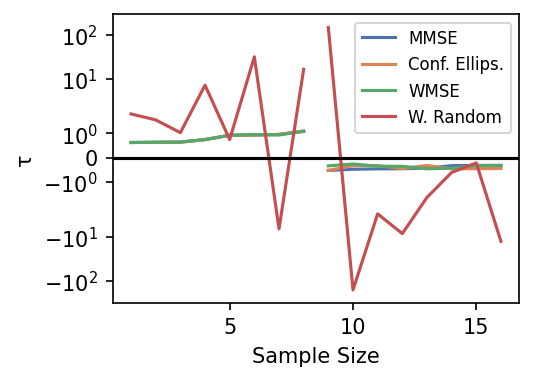
\includegraphics[width=\columnwidth]{figures/proj1/plots/LS_threshold_real/weather_45_bandwidth_8_thresholds_LS.png}}
    \caption{Weather}%
    \label{snr_Weather}%
    \end{subfigure}
    \caption{$\tau(\set{S},v)$ for real world datasets under LS and full-band noise}
\label{LS_SNR_Threshold_plots_all_real}
\end{figure}

\begin{figure}%
    \centering
    \begin{subfigure}{0.31\columnwidth}
    \resizebox{\width}{0.62\columnwidth}{
    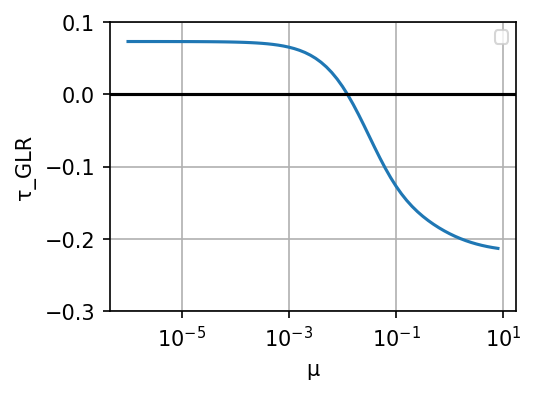
\includegraphics[width=\columnwidth]{figures/proj1/plots/GLR_threshold_real/fmri_subsample_500_GLR_threshold_fb.png}}
    \caption{FMRI}
    \label{tau_GLR_fmri}
    \end{subfigure}
    \begin{subfigure}{0.31\columnwidth}
    \resizebox{\width}{0.62\columnwidth}{
    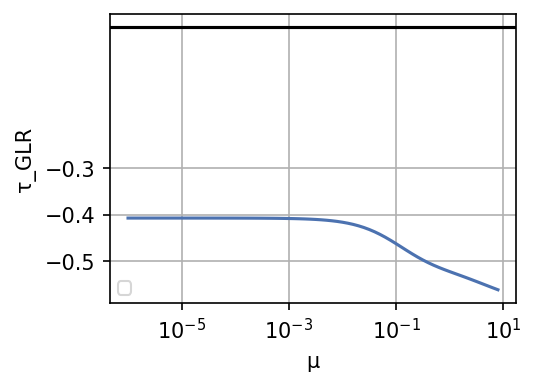
\includegraphics[width=\columnwidth]{figures/proj1/plots/GLR_threshold_real/weather_GLR_threshold_fb.png}}
    \caption{Weather}%
    \label{tau_GLR_weather}%
    \end{subfigure}
    \caption{$\tau_{GLR}$ for real world datasets}
\label{GLR_Threshold_plots_real}
\end{figure}


\begin{figure*}%
    \centering
    \begin{subfigure}{0.3\columnwidth}
    \resizebox{\width}{0.62\columnwidth}{
    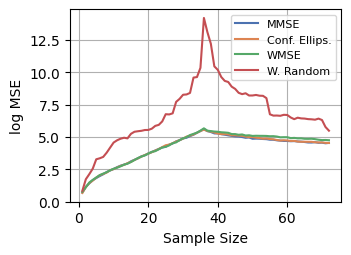
\includegraphics[width=\columnwidth]{figures/proj1/plots/LS_MSE_real/fmri_subsample_500_367_bandwidth_36_SNRdbs_-10.0_samps_72_fb_blsig_MSE_LS.png}}
    \caption{FMRI, SNR = $10^{-1}$}
    \label{fmri_MSE_subfiga}
    \end{subfigure}\hfill
    \begin{subfigure}{0.3\columnwidth}
    \resizebox{\width}{0.62\columnwidth}{
    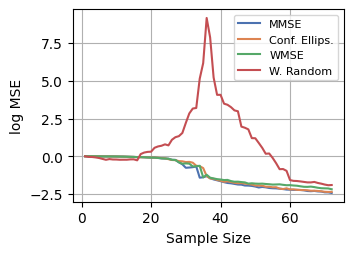
\includegraphics[width=\columnwidth]{figures/proj1/plots/LS_MSE_real/fmri_subsample_500_367_bandwidth_36_SNRdbs_20.0_samps_72_fb_blsig_MSE_LS.png}}
    \caption{FMRI, SNR = $10^{2}$}%
    \label{fmri_MSE_subfigb}%
    \end{subfigure}\hfill%
    \begin{subfigure}{0.3\columnwidth}
    \resizebox{\width}{0.62\columnwidth}{
    \includegraphics[width=\columnwidth]{figures/proj1/plots/LS_MSE_real/fmri_subsample_500_367_bandwidth_36_SNRdbs_100.0_samps_72_fb_blsig_MSE_LS.png}}
    \caption{FMRI, SNR = $10^{10}$}%
    \label{fmri_MSE_subfigc}%
    \end{subfigure}%
    \hfill
    \begin{subfigure}{0.3\columnwidth}
    \resizebox{\width}{0.62\columnwidth}{
    \includegraphics[width=\columnwidth]{figures/proj1/plots/LS_MSE_real/weather_45_bandwidth_8_SNRdbs_-10.0_samps_16_fb_blsig_MSE_LS.png}}
    \caption{Weather, SNR = $10^{-1}$}
    \label{weather_MSE_subfiga}
    \end{subfigure}\hfill
    \begin{subfigure}{0.3\columnwidth}
    \resizebox{\width}{0.62\columnwidth}{
    \includegraphics[width=\columnwidth]{figures/proj1/plots/LS_MSE_real/weather_45_bandwidth_8_SNRdbs_20.0_samps_16_fb_blsig_MSE_LS.png}}
    \caption{Weather, SNR = $1$}%
    \label{weather_MSE_subfigb}%
    \end{subfigure}\hfill%
    \begin{subfigure}{0.3\columnwidth}
    \resizebox{\width}{0.62\columnwidth}{
    \includegraphics[width=\columnwidth]{figures/proj1/plots/LS_MSE_real/weather_45_bandwidth_8_SNRdbs_100.0_samps_16_fb_blsig_MSE_LS.png}}
    \caption{Weather, SNR = $10^{10}$}%
    \label{weather_MSE_subfigc}%
    \end{subfigure}%
    \caption{Average MSE under LS on real world datasets and full-band noise }
\label{LS_real_MSE_fig}
\end{figure*}


We first discuss the plots of $\tau$ and $\tau_{GLR}$ for real world datasets. In practice, one cannot know for sure what the signal model of a real world signal is; however, computation of $\tau$ is dependent on our choice of theoretical signal model. We have therefore computed $\tau$ under the signal model assumptions given in Section \ref{sec:signal_model}.  
}
%By Proposition \ref{propn:averages_generalise_to_forall}, we know that there is a threshold $\tau > 0$ whenever $\tau$ is positive under our bandlimited signal model. This means that we have proven the sign of $\tau$ in \ref{LS_SNR_Threshold_plots_all_real} is correct, even though our assumption that the covariance of the signal model is $\projbl$ may not hold. We validate the accuracy of the value of our computed $\tau(\set{S},v)$ in our discussion of the MSE plots.
{\color{black}
\subsubsection{$\tau$ plots (LS)}
We examine Fig. \ref{LS_SNR_Threshold_plots_all_real}. By Proposition \ref{propn:averages_generalise_to_forall}, the sign of $\tau(\set{S},v)$ we have plotted is provably correct for \emph{any} signal model $\tau$. 
We validate the actual value of $\tau$ with MSE experiments (Figs. \ref{LS_real_MSE_fig} \& \ref{GLR_real_MSE_fig}).


\subsubsection{MSE plots (LS)}
At high noise levels, Figs. \ref{weather_MSE_subfiga} and \ref{fmri_MSE_subfiga} show a $\Lambda$-shaped MSE, validating Proposition \ref{propn:averages_generalise_to_forall} applied to Remark \ref{remark:LS_error_lambda_shaped}. 

In both plots in Fig. \ref{LS_SNR_Threshold_plots_all_real}, all of the lines are above $10^{-1}$. This corresponds to Fig. \ref{weather_MSE_subfiga} and Fig. \ref{fmri_MSE_subfiga} being $\Lambda$-shaped. In Fig. \ref{LS_SNR_Threshold_plots_all_real}, all of the lines are under $10^{10}$. This correponds to Fig. \ref{weather_MSE_subfigc} and Fig. \ref{weather_MSE_subfigc} being decreasing, which we observe.

In Fig. \ref{snr_FMRI}, we see the red line (Weighted Random sampling) is broadly above $10^2$ and the other lines (MMSE, WMSE and Confidence Ellipsoid Sampling) are below $10^2$. This corresponds to the red MSE line being $\Lambda$-shaped and the other lines decreasing in Fig. \ref{fmri_MSE_subfigb}. 

In Fig \ref{snr_Weather} all lines are below $10^{2}$ and so we expect at $\text{SNR}=10^{2}$ for all lines to be decreasing. For MMSE, WMSE and Confidence Ellipsoid sampling this is consistent with Fig. \ref{weather_MSE_subfigb}; however, it is clear our covariance assumption has underestimated $\tau$ for Weighted Random Sampling as the red line is $\Lambda$-shaped in Fig. \ref{weather_GLR_MSE_subfigb}.


We see that the real world results are broadly in line with the synthetic experiments, validating our use of the signal model presented in Section \ref{sec:signal_model} to calculate $\tau$ for LS.

\section{Discussion}
In this paper we studied the impact of sample size on linear reconstruction of noisy $k$-bandlimited graph signals. We showed theoretically and experimentally, in the same settings as much of the sample set selection literature, that reconstruction error is not always monotonic in sample size, i.e., at sufficiently low SNRs, reconstruction error can sometimes be improved by \emph{reducing} sample size. %, even if the sample set was picked by a greedy optimal sampling scheme given a fixed sample size.
Our finding reveals that existing results in the literature for the noiseless setting may not necessarily generalise to the noisy case,  even when considering regularised reconstruction methods. It also demonstrates the need to consider both optimal sample size selection and reconstruction methods at the same time, and motivates assessment of noise levels in datasets to do so. %For example, the limitation of ordinary LS reconstruction may be mitigated by regularisation schemes such as that proposed in \cite{chamon2017greedy}.
% This paper demonstrates the potential limitation of a focus on efficient optimal sample set selection, and the importance of both constructing efficient regularised reconstruction operators in reconstructing graph signals. Furthermore, it demonstrates the need for sample size bounds and guidelines specifically catering to the noisy reconstruction case with operators used in the literature, rather than optimal Bayesian operators.

\xd{One practical implication of our theoretical results is that it can provide useful guidance on how to make use of the sampling budget available. For example, if one is aware of potentially high noise present in the observed signals, to minimise MSE under LS reconstruction, it might be preferable to not use all of the provided sampling budget.}

\xd{Another use case could be a practical sampling algorithm, for both the LS and GLR reconstructions. For LS reconstruction, if one has chosen $k$ or fewer nodes by some noiseless-optimal scheme, one can calculate $\tau(\set{S},v)$ for each element of $\set{S}$, remove $v$ if $\text{SNR} < \tau(\set{S},v)$, and repeat until it is no longer possible to find a node $v$ in our remaining set $\set{S}_{rem}$ where $\text{SNR} < \tau(\set{S}_{rem},v)$.}

\xd{For the GLR reconstruction, with a fixed $\mu$ and belief that the signal model in Section \ref{sec:every_x} applies (the latter could be assessed based on past observations and is required for computation of the SNR threshold $\tau$), then our results suggest the following sampling algorithm can be considered. Given the graph structure, before observing any nodes:
\begin{enumerate}
    \item Check whether condition \ref{eq:GLR_exist_thm_B_constraint} in Theorem \ref{thm:main_GLR_exist} applies (this only depend on graph structure);
    \item If they do, compute $\tau_{GLR}$;
    \item If it is believed that $\text{SNR} < \tau_{GLR}$ holds, sample $m_{opt}$ (approximately $\sqrt{N}$) nodes at random and reconstruct from those nodes.
\end{enumerate}}

We finally remark that future work includes extending the analysis on GLR to the normalised graph Laplacian, providing bounds on $\xi_2$ for LS, analysing other graph models such as Ring graphs or studying a mode detailed ``early-stopping'' mechanism in sequential sampling schemes that do not use the full sample budget.

%%% LS plots


\chapter{\label{ch:proj1_GLR}On the Impact of Sample Size in Reconstructing Noisy Graph Signals: Graph Laplacian Regularised Reconstruction}

\section{Introduction}




\begin{table}[h]
\caption{Structure of Theoretical Results}
\centering
\begin{tabular}{@{} l   c c @{}}
\toprule
 & \multicolumn{2}{c}{GLR} \\
\cmidrule(lr){2-3}
{} & Full-band Noise & Bandlimited Noise \\
\midrule
\emph{Simplification}  & {$\set{N}$ vs $\set{S}$}   & {$\set{N}$ vs $\set{S}$}  \\
\midrule
\emph{Characterisation} & {Corr \ref{corr:main_GLR_iff}} & {Corr \ref{corr:main_GLR_iff}} \\
\midrule
\emph{Existence} & Thm \ref{thm:main_GLR_exist} & Thm \ref{thm:main_GLR_bl}  \\
\midrule
\emph{Asymptotics} &  Propn \ref{propn:GLR_big_N} & Propn \ref{propn:GLR_big_N_bl}\\
\bottomrule
\end{tabular}
\label{tbl:general_theory}
\end{table}

\section{Theoretical Results}
\subsection{GLR with full-band noise}
\label{sec:GLR_full_band}
In this subsection, we show how decreasing sample size can decrease MSE under GLR reconstruction and full-band noise. 


\subsubsection{\bs{Overview and Simplification}}
We start by trying to simplify Theorem \ref{main_general}. Table \ref{tbl:GLR_Reconstruction_Delta} contains no $\times$ scenarios and so the `single vertex' simplification cannot eliminate any conditions in Theorem \ref{main_general}: surprisingly, $\matr{R}_{\set{S} \backslash \{ v \}}$ can be \emph{less} biased than $\matr{R}_{\set{S}}$ for GLR, which can be observed experimentally.
Instead, as we focus on tractability and showing that it is possible to reduce sample size to reduce MSE, rather than fully characterizing all such cases, we pick a situation where $\Delta_{1} \geq 0$ so we can simplify Theorem \ref{main_general}. Specifically, we compare the full observation set $\set{S}=\set{N}$ to a subset of it, which we call the `full observation' simplification. As it is hard to interpret what reconstruction means under full observation \cite{chen2017GLRbias}, our results should be understood as approximately showing that reducing the sample size from nearly full observation to some smaller size may reduce MSE.

Our approach is then as follows. We first characterise under exactly which conditions a sample set $\set{S} \subset \set{N}$ is better than $\set{N}$ (Corollary \ref{corr:main_GLR_iff}). We then show that these conditions must occur if certain graph invariants hold (Theorem \ref{thm:main_GLR_exist}). Finally, we analyse the parameters in Theorem \ref{thm:main_GLR_exist} to obtain a `suggested sample size' (Remark \ref{remark:mopt}) and show the conditions still occur as $N \to \infty$ (Proposition \ref{propn:GLR_big_N}). 

\subsubsection{\bs{Characterisation}}
We first present the following Corollary of Theorem \ref{main_general}.

\begin{corollary}
    \label{corr:main_GLR_iff}
    Assume GLR and that $k > 1$. Consider a non-empty sample set $\set{S} \subset \set{N}$.  Then 
    \begin{equation}
        \tau(\set{N},\set{S}^{c}) = \frac{k}{N} \cdot \frac{\Delta_{2}(\set{N},\set{S}^{c})}{-\Delta_{1}(\set{N},\set{S}^{c})} \label{eq:main_GLR_simplified_tau}
    \end{equation}
    and $\set{S}$ is better than $\set{N}$ if and only if one of the following conditions is met:
        \begin{subnumcases}{ \label{eq:GLR_corol_iff_overall} }
        \text{SNR} < \tau(\set{N}, \set{S}^{c}) &and $ \msubgen[\set{S}^{c},\{2,\ldots,k\}]{\matr{U}} \neq \matr{0}$ \label{eq:GLR_corol_iff}\\
        0 < \Delta_2(\set{N},\set{S}^{c}) &and $ \msubgen[\set{S}^{c},\{2,\ldots,k\}]{\matr{U}} = \matr{0}$. \label{eq:GLR_corol_iff_weird}
\end{subnumcases}
where $\msubgen[\set{S}^{c}, \{2,\ldots,k\}]{\matr{U}} = \vect{0}$ corresponds to any $k$-bandlimited signal always being constant on all of $\set{S}^{c}$.
\end{corollary}
\begin{proof}[Proof Sketch]
    We use Cauchy-Schwartz and Lemma \ref{lemma:GLR_full_observation_MSE} to lower bound $\xi_{1}(\set{S})$ and show that either all $k$ columns of $\matrsubU{N}$ are eigenvectors of $\proj{S} + \mu\matr{L}$ (which is exactly when $\msubgen[\set{S}^{c},\{2,\ldots,k\}]{\matr{U}} = \matr{0}$) and $\Delta_{1}(\set{N},\set{S}^{c}) = 0$, corresponding to (\ref{eq:GLR_corol_iff_weird}), or $\Delta_{1}(\set{N},\set{S}^{c}) < 0$, corresponding to (\ref{eq:GLR_corol_iff}). We then apply Theorem \ref{main_general}. See Appendix \ref{app:proof_main_GLR_iff} for a full proof.
\end{proof}


We now explain the conditions in Corollary \ref{corr:main_GLR_iff}. Condition (\ref{eq:GLR_corol_iff}) corresponds to the single case we see in Corollary \ref{main_ls}. Condition (\ref{eq:GLR_corol_iff_weird}) is more of an edge case,  e.g., if $\lambda_{k} < N$ and every vertex in $\set{S}^{c}$ has degree $N-1$ \cite[Corollary 2.3]{merris1998laplacian}. In (\ref{eq:GLR_corol_iff_weird}), $\msubgen[\set{S}^{c}, \{2,\ldots,k\}]{\matr{U}} = \vect{0}$ means any $k$-bandlimited signal will be constant on all of $\set{S}^{c}$. Our proof shows that in the noiseless case this implies that observing $\set{S}^{c}$ will not improve the MSE, i.e., $\text{MSE}_{\set{S} \cup \set{T}_{c}} = \text{MSE}_{\set{S}}$ for any $\set{T}_{c} \subseteq \set{S}^{c}$. %which means that no information can be gained by observing $\set{S}^{c}$ for a $k$-bandlimited signal apart from the component of the signal which is constant (which corresponds to the lowest graph frequency). For GLR reconstruction in the noiseless case, this knowledge does not aid reconstruction as GLR can always perfectly reconstruct constant signals, and unlike LS it cannot use this knowledge to improve reconstruction of the other components of the bandlimited signal. Therefore, if $\msubgen[\set{S}^{c},\{2,\ldots,k\}]{\matr{U}} = \matr{0}$, observing $\set{S}^{c}$ does not improve the expected MSE under GLR reconstruction in the noiseless case (see Appendix \ref{subapp:GLR_iff_proof:idempotent} for a symbolic proof of this statement). 
The other condition in (\ref{eq:GLR_corol_iff_weird}), i.e., $0 < \Delta_2(\set{N},\set{S}^{c})$, corresponds to an increase in sensitivity to noise from reconstructing from those additional vertices. Therefore, condition (\ref{eq:GLR_corol_iff_weird}) says that if $\set{S}^{c}$ reveals nothing new about the underlying signal and also makes the reconstruction more sensitive to noise, one should not observe $\set{S}^{c}$ and only observe $\set{S}$.


%Instead of exactly characterising the behaviour on removing a single vertex from an arbitrary sample set $\set{S}$, we proceed with our `bound' proof strategy. We consider removing multiple vertices from the full observation set $\set{N}$. We use Theorem \ref{main_general} by bounding $\tau(\set{N},\set{S}^{c})$. We do so by bounding $\xi_{i}(\set{S})$ and $\xi_{i}(\set{N})$, and thence bounding $\Delta_{i}(\set{N}, \set{S}^{c})$. This gives a characterisation of when removing all but a sample set $\set{S}$ improves $\set{N}$. We call this bound $\tau_{lb}$.

\subsubsection{\bs{Existence}}
Like Corollary \ref{main_ls}, Corollary $\ref{corr:main_GLR_iff}$ does not show that any set $\set{S}$ is ever better than $\set{N}$, i.e., that $\tau(\set{N},\set{S}^{c}) > 0$ ever happens. {\color{black} As described in Section \ref{sec:every_x}, we will find $\set{S}$ s.t. $\Delta_{2}(\set{N},\set{S}^{c}) > 0$. We illustrate our proof method in Fig.~\ref{fig:GLR_diagram}.

\begin{figure}[t]
    \centering
    %\resizebox{\width}{0.75\columnwidth}
    \resizebox{0.75\width}{0.75\height}
    {\includegraphics[width=\columnwidth]{figures/proj1/plots/GLR_diagram/diagram_GLR.png}}
    \caption{Proof direction to show $\Delta_{2}(\set{N},\set{S}^{c}) > 0$}
    \label{fig:GLR_diagram}
\end{figure}

\noindent Fundamentally, our approach rests on the fact that $\xi_{2}$, which is approximately proportional to $\text{MSE}_{\set{S}}$ at high noise levels, is  approximately U-shaped, and we can use an upper bound to approximate the minimum and thus bound $\Delta_{2}(\set{N},\set{S}^{c})$ below. Explicitly, our method to show $\Delta_{2}(\set{N},\set{S}^{c}) > 0$ is:
\begin{enumerate}
    \item Find an upper bound $B(\cdot)$ for $\xi_{2}(\set{S})$ that only depends on $\matr{L}$ and $|\set{S}|$, not on $\mu$ or the choice of $\set{S}$.
    \item Find the sample size $m_{opt}$ that minimises the bound and show $m_{opt} < N$.
    \item Identify when $\xi_{2}(\set{N}) - B(m_{opt}) > 0$ (this is the `$\Delta_{2}$ bound' in Fig. \ref{fig:GLR_diagram}). As this quantity is a lower bound for $\Delta_{2}(\set{N},\set{S}^{c})$ this shows that $\Delta_{2}(\set{N},\set{S}^{c})>0$ for any $\set{S}$ of size $m_{opt}$.
    \item Bound $\Delta_{1}$ using the same tools and use these to lower bound $\tau(\set{N}, \set{S}^{c})$
\end{enumerate}
We see that $m_{opt}$ suggests an `optimal sample size', in the sense that the $\xi_{2}$ upper bound approximates $\xi_{2}$, and we can optimise it as a surrogate. Following step 1, we now bound $\xi_{2}(\set{S})$.

\iffalse
To show that $\tau$ can be positive under GLR, we bound it from below similarly to Theorem \ref{thm:noiseless_optimality_means_noise_sensitivity}.{\color{black} We start with a weaker, easier-to-understand version of the full theorem:
\fi

\begin{lemma}
\label{lemma:GLR_xi_2_bound_main}
    Let $\lambda_{i}$ be the eigenvalues of $\matr{L}$, the combinatorial Laplacian. Let $|\set{S}| = m$. Then
    \begin{align}
        \xi_{2}(\set{S}) &\leq r\frac{N}{m} + \sum_{i=2}^{m} \omega\left(\max\left[1,\frac{\lambda_{N+2-i}}{\lambda_{i}}\right]\right)  \label{eq:xi_2_GLR_bound_strong}
        \\ 
        &\leq r\frac{N}{m} + r(m -1) . \label{eq:xi_2_GLR_bound_weak}
    \end{align}
    where we define $B(m)$ to be the RHS of (\ref{eq:xi_2_GLR_bound_strong}) and where
    \begin{align}
        \omega(x) &= \frac{1}{4}\left(\sqrt{x}+ \frac{1}{\sqrt{x}} \right)^{2}, \quad
        r = \omega\left(\frac{\lambda_{N}}{\lambda_{2}}\right)
    \end{align}
   and the summation in (\ref{eq:xi_2_GLR_bound_strong}) is 0 if $m = 0$ or $1$. 
    
\end{lemma}
\begin{proof}
    Decompose $\matr{R}_{\set{S}}$ and apply Kantorovich's inequality. See Appendix \ref{app:proof_unif_ub_xi_2}.
\end{proof}

The function $\omega$ arises from the Kantorovich inequality, commonly used in variance bounds \cite{khatri1982some, householder1965kantorovich}. $\omega$ is an increasing function and for $x>1, \omega(x) \leq x$; this means $r$ increases with $\frac{\lambda_{N}}{\lambda_{2}}$. We discuss $r$ in more detail in Appendix \ref{app:GLR_sensitivity}.

As mentioned, in step 4 we need a bound on $\xi_{1}(\set{S})$ to lower bound $\tau(\set{N},\set{S}^{c})$. The shape and accuracy of this bound do not affect the core of our argument, only how tight our approximation of $\tau$ is. Therefore, we leave it in Appendix \ref{app:proof_unif_ub_xi_1_MSE}; the term $B_{k}(m)$ it introduces in the proof is a tightening of $B(m)$ ($B_{k}(m) < B(m)$) and is explained in Appendix  \ref{app:GLR_bandlimited}.

Following steps 2, 3 and 4 using the bound $B(m)$ in Lemma \ref{lemma:GLR_xi_2_bound_main} yields: 

\begin{theorem}
\label{thm:main_GLR_exist}
{\color{black} Let $B(m)$ be defined as in Lemma \ref{lemma:GLR_xi_2_bound_main} and let $m_{opt}$ be the sample size minimising $B$.
    \begin{flalign}
        &\text{If} \hspace{0.35\columnwidth} B(m_{opt}) < N& \label{eq:GLR_exist_thm_B_constraint}
    \end{flalign}
then $m_{opt} < \lceil\frac{N+1}{2}\rceil$. Furthermore, $\exists \mu_{ub} > 0$ and $\tau_{GLR}(\mu) > 0$ s.t. under GLR with parameter $\mu \in (0, \mu_{ub})$,
\begin{flalign}
        &\text{if} \hspace{0.3\columnwidth} \textrm{SNR} < \tau_{GLR}(\mu)&
    \end{flalign}

    \noindent then,  \emph{any} sample set $\set{S}$ of size $m_{opt}$ is better than $\set{N}$.}
\end{theorem}
\begin{proof}[Proof Sketch] 
We prove that for any $\mu$, $\xi_{1}(\set{S}) \leq k + B_{k}(m)$ and $\xi_{2}(\set{S}) \leq B(m)$ via Lemmas \ref{lemma:GLR_xi_2_bound_main} and \ref{lemma:GLR_xi_2_bound_main_bl}. We also show $\xi_{1}(\set{N}) = \sum_{i=1}^{k} \left(1 - \frac{1}{1+\mu\lambda_{i}}\right)^{2}$ and $\xi_{2}(\set{N}) = \sum_{i=1}^{N} \left({1+\mu\lambda_{i}}\right)^{-2}$.
We use these to bound $\Delta_{i}$, and finally apply Corollary \ref{corr:main_GLR_iff} as our conditions mean $\Delta_{2}(\set{N},\set{S}^{c}) > 0$.  See Appendix \ref{app:Proof_thm_main_GLR_exist} for a full proof.
\end{proof}
}
 We contrast Theorems \ref{thm:noiseless_optimality_means_noise_sensitivity} and \ref{thm:main_GLR_exist}. Theorem \ref{thm:noiseless_optimality_means_noise_sensitivity} provides necessary and sufficient conditions. Theorem  \ref{thm:main_GLR_exist}, while still useful, only provides sufficient conditions. 
 Theorem \ref{thm:noiseless_optimality_means_noise_sensitivity} applies to any graph, but only to sample sets chosen under noiseless-optimal sampling schemes, while Theorem \ref{thm:main_GLR_exist} has no requirement on sampling schemes, but only applies to graphs which fulfill certain graph invariants. % for when a subset is better than a sample set of any size chosen under sequential noiseless-optimal sampling schemes under LS. Theorem \ref{thm:main_GLR_exist} only provides sufficient conditions for when removing samples from the full observation set $\set{N}$ reduces MSE under GLR. In this sense, Theorem \ref{thm:main_GLR_exist} is a weaker (nevertheless still useful) result.
 %Finally, both theorems require no constraints on the set of nodes removed for their results to hold.

{\color{black}
Because of the difficulty in writing down an analytic form for $m_{opt}$, the parameters in Theorem \ref{thm:main_GLR_exist} -- $m_{opt}$, $\mu_{ub}$ and $\tau_{GLR}$ -- are difficult to analyse. To better understand  we present a version of Theorem \ref{thm:main_GLR_exist} instead based on  
the weaker bound (\ref{eq:xi_2_GLR_bound_weak}). This bound is a linear transformation of $\frac{N}{m} + m$ and so is clearly U-shaped and has an minimum at $m=\sqrt{N}$, and thus following steps 2, 3 and 4 yields the following proposition:

\begin{propn}
\label{propn:GLR_simple}
    Let $\bar{\lambda} = \frac{1}{N}\sum_{i=1}^{N}\lambda_{i}$ be the mean eigenvalue of $\matr{L}$ and let $r$ be defined as in Lemma \ref{lemma:GLR_xi_2_bound_main}.  
    \begin{flalign}
        &\text{If} \hspace{0.35\columnwidth} 2r\sqrt{N} < N& \label{eq:weak_GLR_constraint}
    \end{flalign}
    Let
    \begin{align}
        \mu_{ub\_weak} &= \bar{\lambda}^{-1}\left(\sqrt[4]{N}\cdot ({2r})^{-\frac{1}{2}} - 1 \right) \\
        \tau_{GLR\_weak} &=  \frac{\sqrt{N}(1 + \mu\bar{\lambda})^{-2} - 2r}{\sqrt{N} + 2r \cdot \frac{N}{k} }
    \end{align}
    then under GLR with parameter $\mu \in (0,\mu_{ub\_weak})$, if
    \begin{equation}
        \text{SNR} < \tau_{GLR\_weak}(\mu)
    \end{equation}
    then \emph{any} sample set $\set{S}$ of size $\lceil\sqrt{N}\rceil$ is better than $\set{N}$.
\end{propn}
\begin{proof}[Proof Sketch]
    We bound $\xi_{1}(\set{S})$ and $\xi_{2}(\set{S})$ in terms of $r\left(\frac{N}{m} + m - 1\right)$, which is minimised at $m = \sqrt{N}$. We explicitly compute $\xi_{i}(\set{N})$ and apply Corollary \ref{corr:main_GLR_iff}. See Appendix \ref{app:proof_propn_GLR_simple} for a full proof.
\end{proof}


%This proposition provides sufficient conditions for reducing sample size to reduce MSE; unlike Theorem \ref{thm:noiseless_optimality_means_noise_sensitivity}, which provides both necessary and sufficient conditions. 

Proposition \ref{propn:GLR_simple} is sufficient to show that decreasing sample size can decrease MSE on a restricted class of graph models (e.g. Erdős–Rényi graphs). 
Proposition \ref{propn:GLR_simple} involves several parameters: $r$, $2r\sqrt{N}$, $\mu_{ub\_weak}$ and $\tau_{GLR\_weak}$ which can be interpreted as graph properties (see Appendix \ref{app:GLR_sensitivity} for a detailed explanation and sensitivity analysis). 


Intuitively, we expect the equivalent parameters in Proposition \ref{propn:GLR_simple} and Theorem \ref{thm:main_GLR_exist} to behave similarly; for $m_{opt}$ to behave like $\left\lceil \sqrt{N} \right\rceil$, for $B(m_{opt})$ to behave like $2r\sqrt{N}$ and for $\mu_{ub}$ and $\tau_{GLR}$ to behave like their weak counterparts. We can explicitly show that $m_{opt}$ is $\mathcal{O}(\sqrt{N})$:

\begin{remark}
\label{remark:mopt}
If condition (\ref{eq:GLR_exist_thm_B_constraint}) in Theorem \ref{thm:main_GLR_exist} holds
    then $m_{opt} \in \left[\left\lfloor\sqrt{N}\right\rfloor, \left\lceil\sqrt{rN}\right\rceil \right]$ and $m_{opt} \leq \lceil\frac{N+1}{2}\rceil$.
\end{remark}
\begin{proof}
    See Appendix \ref{app:proof_of_remark_GLR_mopt}.
\end{proof}

}


%We now exactly write down the MSE when $|\set{S}| = N$:

\iffalse
\begin{theorem}
\label{thm:main_GLR_exist}
{\color{black}
Let $0 = \lambda_{1} < \lambda_{2} \leq \ldots \leq \lambda_{N}$ be the eigenvalues of $\matr{L}$ and let
\begin{align}
    %r_{i} &= \left(\frac{1}{2}\sqrt{ \frac{\lambda_{N+i-1}}{\lambda_{i+1}}} +
    r_{i} &= \frac{(\lambda_{i+1} + \lambda_{N+1-i})^{2}}{4\lambda_{i+1}\lambda_{N+1-i}}, \quad r = r_{1} = \frac{(\lambda_{2} + \lambda_{N})^{2}}{4\lambda_{2}\lambda_{N}}, \\
 %\frac{(\lambda_{i+1}+\lambda_{N+1-i})^{2}}{4\lambda_{i+1}\lambda_{N+1-i}} \\
    \rho(m) &= \begin{dcases}
        \sum^{m}_{i=1} r_{i} & \textrm{if }2m \leq N \\
        (2m - N) + \rho\left((N-1)-m\right)    & \textrm{otherwise}
    \end{dcases},\\ 
    B(m) &= \frac{rN}{m} + \rho({m-1}) 
\end{align}
}
    For any sample size $ 0 < m  < N$, let
    \begin{align}
        \mu_{ub}(m) &= \frac{N}{\trace{\matr{L}}} \left( \sqrt{\frac{N}{B(m)}}  -1 \right) \\
        \tau_{{bound}}(\mu,m) &= \frac{\frac{1}{N}\sum_{i=1}^{N}\left({1 + \mu \lambda_{i}}\right)^{-2} - \frac{B(m)}{N}}{1 + \frac{B(m)}{k} - \frac{1}{k}\sum_{i=1}^{k}\left( 1 - \frac{1}{1 + \mu \lambda_{i}}\right)^{2} }.
    \end{align}
    {\color{black}
    Under GLR with parameter $\mu$ where $0 <\mu < \mu_{ub}(m)$,
    \begin{flalign}
        &\text{if} \hspace{0.35\columnwidth} B(m) < N& \label{eq:GLR_exist_thm_B_constraint} \\
        &\text{and} \hspace{0.3\columnwidth} \textrm{SNR} < \tau_{lb}(\mu,m)&
    \end{flalign}
    then,  \emph{any} sample set $\set{S}$ of size $m$ is better than $\set{N}$.}
\end{theorem}
\begin{proof}[Proof Sketch] 
We prove that  for any $\mu$, $\xi_{1}(\set{S}) \leq k + B(m)$ and $\xi_{2}(\set{S}) \leq B(m)$. We also show $\xi_{1}(\set{N}) = \sum_{i=1}^{k} \left(1 - \frac{1}{1+\mu\lambda_{i}}\right)^{2}$ and $\xi_{2}(\set{N}) = \sum_{i=1}^{N} \left({1+\mu\lambda_{i}}\right)^{-2}$.
We use these to bound $\Delta_{i}$, and finally apply Corollary \ref{corr:main_GLR_iff} as our conditions mean $\Delta_{2}(\set{N},\set{S}^{c}) > 0$. See Appendix \ref{app:Proof_thm_main_GLR_exist} for a full proof.
\end{proof}
\fi


%{\color{black}Finally, we would like to experimentally see what our bound looks like and how it corresponds to MSEs. }
The proof of Theorem \ref{thm:main_GLR_exist} leads to an upper bound of $\text{MSE}_{\set{S}}$. {\color{black} We present this upper bound to link the experiments in Section \ref{sec:experiments} with Fig. \ref{fig:GLR_diagram}, which can be considered to be the case where $\sigma^{2} \to \infty$.
\begin{corollary}
\label{corr:unif_ub_xi_1_MSE}
    Let $B(m)$ be defined as in Lemma \ref{lemma:GLR_xi_2_bound_main} and $B_{k}(m)$ be defined as it will be in Lemma \ref{lemma:GLR_xi_2_bound_main_bl}. 
    
    For a sample set $\set{S}$ of size $m$,
    \begin{align}
    \textrm{MSE}_{\set{S}} &\leq (k + B_{k}(m)) + \sigma^{2} \cdot B(m). \label{eq:unif_ub_MSE}
    \end{align}
\end{corollary}
\begin{proof}
By Lemma \ref{lemma:GLR_xi_2_bound_main} \iffalse in Appendix \ref{app:proof_unif_ub_xi_2},\fi $\xi_{2}(\set{S}) \leq B(m)$. By Lemma \ref{lemma:unif_ub_xi_1_GLR} in Appendix \ref{app:proof_unif_ub_xi_1_MSE}, $\xi_{1}(\set{S}) \leq k + B_{k}(m)$. Combining these using (\ref{eq:xi_decomp}) gives the bound.
\end{proof}
}

 
\iffalse
\begin{remark}
\label{remark:mopt}
Assume $N > 4$ and define
\begin{align}
    m_{opt} = \min \argmin_{m \in [1,N] \cap \mathbb{Z}} B(m).
\end{align}
    \iffalse
    $ m_{opt}$ exists where
    \begin{equation}
        m_{opt} = \min \left\{m\enskip \middle| \enskip \frac{m(m+1)}{N} > \frac{r}{r_{m}} \right\}.
    \end{equation}
    \fi
    If (\ref{eq:GLR_exist_thm_B_constraint}) in Theorem \ref{thm:main_GLR_exist} holds for some $m \in [1,N]$
    then 
    \begin{itemize}
        \item Condition (\ref{eq:GLR_exist_thm_B_constraint}) holds at a sample size of $m_{opt}$ .
        \item $\mu_{ub}(m)$ and $\tau_{lb}(\mu,m)$ are both maximised at $m=m_{opt}$.
        \item The MSE upper bound in Corollary \ref{corr:unif_ub_xi_1_MSE} is minimised at a sample size of $m_{opt}$.
        \item $m_{opt} \in \left[\left\lfloor\sqrt{N}\right\rfloor, \left\lceil\sqrt{rN}\right\rceil \right]$ and $m_{opt} \leq \frac{N}{2}$.
    \end{itemize}
\end{remark}
\begin{proof}
    See Appendix \ref{app:proof_of_remark_GLR_mopt}.
\end{proof}
\fi




\iffalse
Theorem \ref{thm:main_GLR_exist} can be better understood by a sensitivity analysis: $r_{i} < r$ implies $\rho(m)$ and $B(m)$ decrease with $r$.
% \begin{remark}
% \label{remark:GLR_sensitivity_analysis}
Therefore for any $m$, as $r$ decreases, both $\mu_{ub}(m)$ and $\tau_{lb}(m)$ increase.
% \end{remark}
% \begin{proof}
    
% \end{proof}

The above results are for a given sample size $m$. We then ask what our results suggest the optimal sample size might be. Noting $B$ may have multiple minima, % and that argmin is a set function, and so using min argmin to select the smallest sample size which is a minimum of $B$, 
we define the following:

%We now ask: if we do not mind what sample size we pick, what can Theorem \ref{thm:main_GLR_exist} tell us?

\iffalse
Based on the above, we define
\begin{align}
    \tau_{GLR}(\mu) = \max_{m} \tau_{lb}(\mu, m) = \tau_{lb}(\mu, m_{opt}).
\end{align}
$\tau_{GLR}(\mu)$ is the largest SNR where by Theorem \ref{thm:main_GLR_exist} we know we can improve $\set{N}$ by reducing sample size. We note that \emph{any} sample set of size $m_{opt}$ suffices. On the other hand, even if $\text{SNR}> \tau_{GLR}$,  a sample set $\set{S}$ of size $m$ selected by an optimal sample scheme could still be better than $\set{N}$.
\fi
\iffalse
Therefore we can show when we can lower the MSE on average by sampling fewer nodes:

\begin{theorem}
\label{thm:main_GLR}
Let $r$ and $\rho$ be defined as in Lemma \ref{lemma:unif_ub_xi_2} and define
    \begin{align}
        m &= \left\lceil \sqrt{rN} \right\rceil \\
        z &= \sqrt{rN} + \rho(m-1).
    \end{align}
    Assume that
   \begin{align}
    N > 2+r \\
     z < N. \label{eq:GLR_b_constraint}
\end{align}
 
    Let 
    \begin{align}
        \mu_{ub} = \frac{N}{\trace{\matr{L}}} \left( \sqrt{\frac{N}{z}}  -1 \right). \label{eq:mu_constraint_GLR}
        \end{align}
    Fix $\mu \in (0, \mu_{ub})$ and let 
        \begin{align}
        \tau_{GLR} &= \frac{\frac{1}{N}\sum_{i=1}^{N}\left(\frac{1}{1 + \mu \lambda_{i}}\right)^{2} - \frac{z}{N}}{1 + \frac{z}{k} - \frac{1}{k}\sum_{i=1}^{k}\left( 1 - \frac{1}{1 + \mu \lambda_{i}}\right)^{2} }
    \end{align}
    
    Assume GLR reconstruction with parameter $\mu$. If
    \begin{equation}
        \textrm{SNR} < \tau_{GLR}
        \label{eq:SNR_constraint_GLR}
    \end{equation}
    then for any vertex observation set $\set{S}$ of size $m$,
    \begin{equation}
        \textrm{MSE}_{\set{S}} < \textrm{MSE}_{\set{N}}.
    \end{equation}
    
\end{theorem}
\begin{proof}[Proof Sketch] By Lemma \ref{lemma:unif_ub_xi_2},  if $|\set{S}| = \left\lceil\sqrt{rN}\right\rceil$,
\begin{equation}
\xi_{2}(\set{S}) \leq z.
\end{equation}
Eq. (\ref{eq:GLR_b_constraint}) $\implies \mu_{ub} > 0$, and after rearranging, $\mu \in (0,\mu_{ub})$ means $\xi_{2}(\set{N}) \geq z \geq \xi_{2}(\set{S})$ by Lemma \ref{lemma:GLR_full_observation_MSE}. We then pick $\tau_{GLR}$ s.t. if $\textrm{SNR} < \tau_{GLR}$ then
\begin{equation}
    \sigma^{2} > \frac{\xi_{1}(\set{S}) - \xi_{1}(\set{N})}{\xi_{2}(\set{N}) - \xi_{2}(\set{S})}
\end{equation}
This implies $\textrm{MSE}_{\set{S}} < \textrm{MSE}_{\set{N}}$.
For full details, see Appendix \ref{app:Proof_main_GLR}.
\end{proof}

\iffalse
While this particular theorem is useful computationally, we present a weaker corollary that is easier to understand and work with theoretically:

\begin{corollary}
    Let $r$ be defined as in Proposition \ref{propn:unif_ub_xi_2}. Suppose that $N > 4$ and that 
    \begin{equation}
        2r < \sqrt{N}
    \end{equation}
     Let 
    \begin{align}
        \mu_{ub} = \frac{N}{\trace{\matr{L}}} \left( {\frac{\sqrt[4]{N}}{\sqrt{2r}}}  -1 \right). 
        \end{align}
    Fix $\mu \in (0, \mu_{ub})$ and let 
        \begin{align}
        \tau_{GLR\_weak} &= \frac{\frac{1}{N}\sum_{i=1}^{N}\left(\frac{1}{1 + \mu \lambda_{i}}\right)^{2} - \frac{2r\sqrt{N}}{N}}{1 + \frac{2r\sqrt{N}}{k} - \frac{1}{k}\sum_{i=1}^{k}\left( 1 - \frac{1}{1 + \mu \lambda_{i}}\right)^{2} }
    \end{align}
    Assume GLR reconstruction with parameter $\mu$. If
    \begin{equation}
        \textrm{SNR} < \tau_{GLR\_weak}
    \end{equation}
    then for any vertex observation set $\set{S}$ of size $\left\lceil \sqrt{N}\right\rceil$,
    \begin{equation}
        \textrm{MSE}_{\set{S}} < \textrm{MSE}_{\set{N}}.
    \end{equation}
\end{corollary}
\fi
\fi
\iffalse
\begin{remark}
    $\tau_{GLR}$ in Theorem \ref{thm:main_GLR} is different in kind to the threshold $\tau(\set{S},v)$ in Corollary \ref{main_ls}. While $\tau(\set{S},v)$ measures what happens to MSE when a specific vertex $v$ is removed from a specific vertex observation set $\set{S}$, $\tau_{GLR}$ is only a function of $\mathcal{G}, \mu, k$, and is not dependent on $\set{S}$.

    Furthermore, the inequalities around $\tau(\set{S},v)$ in Corollary \ref{main_ls} are necessary and sufficient, while the inequalities in Theorem $\ref{thm:main_GLR}$ are only sufficient; if $\textrm{SNR} > \tau(\set{S},v)$ then under LS reconstruction removing $\{v\}$ from $\set{S}$ will not decrease MSE; whereas even if $\textrm{SNR} > \tau_{GLR}$ under GLR reconstruction reducing the sample size might still decrease MSE.
\end{remark}
\fi
\iffalse
\begin{remark}
    Unlike in Corollary \ref{main_ls}, the inequalities in Theorem \ref{thm:main_GLR} are sufficient but not necessary. For example, while $\textrm{SNR} < \tau_{GLR}$ guarantees that on average the MSE is lowered by sampling $m$ nodes, it is possible that even with  $\textrm{SNR} > \tau_{GLR}$ we can find an observation set $\set{S}$ s.t. $|\set{S}| < N$ and $\textrm{MSE}_{\set{S}} < \textrm{MSE}_{\set{N}}$.
\end{remark}
\fi

Note that $m_{opt}$, $\mu_{ub}(m_{opt})$ and $\tau_{GLR}$ are graph invariants and they quantify amenability to signal reconstruction with low sample sizes at high noise. 
\iffalse
To better understand Theorem \ref{thm:main_GLR_exist}, we present results around what the parameters mean and some sensitivity analyses.
\begin{remark}
\label{remark:GLR_sensitivity_analysis}
 As $r$ decreases:
 \begin{itemize}
     \item $\mu_{ub}$ increases
     \item $\tau_{lb}$ increases
     \item $m_{opt}$ decreases to $\left\lceil\sqrt{N}\right\rceil$.
 \end{itemize}
 The above follows from the fact that $r_{i} < r$ and so $\rho(m)$ and $B(m)$ are decreasing in $r$.
\end{remark}
\fi
As $r$ decreases, $m_{opt}$ decreases to $\sqrt{N}$. This and our sensitivity analysis show that graphs with low $r$ are more amenable to reconstruction with fewer observations via GLR\footnote{We give some intuition for $r$: low $r$, equivalent to low $\frac{\lambda_{N}}{\lambda_{2}}$, is a known condition in the Network Sychronisation literature which allows for dynamic oscillators on a network to synchronise \cite{barahona2002synchronization}.}. %In the proof of Proposition \ref{propn:unif_ub_xi_2}, $r$ is used to bound the off-diagonal elements of $\matr{L}^{\dagger}$ by how spread out the eigenvalues are. 
\fi
\iffalse
In the literature on Network Synchronisation \cite{barahona2002synchronization}, small $\frac{\lambda_{N}}{\lambda_{2}}$ is a condition which allows for dynamic oscillators on a network to synchronise. As $r$ is an increasing function of $\frac{\lambda_{N}}{\lambda_{2}} $  we see that $\frac{\lambda_{N}}{\lambda_{2}}$ being small also allows for better reconstruction with fewer observations under looser conditions.
\fi

\subsubsection{\bs{Asymptotics}}
Finally, we consider the case of large graphs.{\color{black} While our sensitivity analysis suggests that $\tau_{GLR} \to 0$ as $N$ gets large, this is an oversimplification from assuming indepence of parameters in our analysis. We present a Proposition to show that that $\tau_{GLR} \not\to 0$ as $N \to \infty$ for ER graphs.
\begin{propn}
\label{propn:GLR_big_N}
For Erdős–Rényi graphs, as $N \to \infty$, condition (\ref{eq:GLR_exist_thm_B_constraint}) in Theorem \ref{thm:main_GLR_exist} holds w.h.p. and $\tau_{GLR}$ tends to a positive constant even under optimal choice of $\mu$ \cite{chen2017GLRbias}.
\end{propn}
\begin{proof}
    Full statement and proof in Appendix 
 \ref{app:Proof_GLR_big_N}.
\end{proof}
}
{\color{black} This shows that reducing sample size can reduce MSE on arbitrarily large graphs under GLR even with optimal $\mu$. 
}
%We analyse Theorem \ref{thm:main_GLR_exist} to show that $\tau_{GLR} \not\to 0$ as $N \to \infty$ and so our analysis is also relevant for large graphs. We only consider Erdős–Rényi graphs to simplify the analysis. 

\subsection{GLR with $k$-bandlimited noise}
\label{sec:GLR_bandlimited}
%As in Section \ref{sec:LS_bandlimited}, we show MSE increasing with sample size is not caused by some sort of interference effect between the high-frequency components of the noise and the bandlimited (low-frequency) signal for GLR by proving a variant of Theorem \ref{thm:main_GLR_exist} for $k$-bandlimited noise.
Once more, one might ask whether the MSE increasing with sample size under GLR is caused by some sort of interference effect between the high-frequency components of the noise and the bandlimited (low-frequency) signal. {\color{black} We present a variant of Theorem \ref{thm:main_GLR_exist} to disprove this.

\subsubsection{\bs{Simplification }} As with the full-band GLR case, we consider when a set $\set{S} \subset \set{N}$ is better than $\set{N}$.
\subsubsection{\bs{Characterisation}}
We first note that Corollary \ref{corr:main_GLR_iff} also applies to the bandlimited case with the appropriate definition of $\Delta_{2}$, providing a full characterisation of when a set $\set{S}$ is better than $\set{N}$ under GLR reconstruction with bandlimited noise.

\subsubsection{\bs{Existence}}
 We now present a bandlimited variant of Lemma \ref{lemma:GLR_xi_2_bound_main}. It can be understood as Lemma \ref{lemma:GLR_xi_2_bound_main} with $\lambda_{N}$ replaced by $\lambda_{k}$.

\begin{lemma}
\label{lemma:GLR_xi_2_bound_main_bl}
    Let $\lambda_{i}$ be the eigenvalues of $\matr{L}$ and let $\omega$ be defined as in Lemma \ref{lemma:GLR_xi_2_bound_main}. Let
    \begin{align}
        r_{bl} &= \omega\left( \frac{\lambda_{k}}{\lambda_{2}}\right) \\
        B_{k}(m) &= r_{bl} \frac{N}{m} + \sum^{m}_{i=1}\omega\left(\max\left[1,\frac{\lambda_{k+2-i}}{\lambda_{i}}\right]\right)
    \end{align}
    where the summation is 0 if $m=0$ or 1. Then
    \begin{align}
        \xi_{2,bl}(\set{S}) &\leq 1 + B_{k}(m) \leq 1 + r_{bl} \left( \frac{N}{m} + m - 1 \right).
    \end{align}
\end{lemma}
\begin{proof}
    We prove a bandlimited variant of the Kantorovich inequality and use the same structure as the proof of Lemma \ref{lemma:GLR_xi_2_bound_main}. See Appendix \ref{app:GLR_bandlimited_lemma_proof}.
\end{proof}

A version of Theorem \ref{thm:main_GLR_exist} follows in the same manner as with full-band noise:

\begin{theorem}
\label{thm:main_GLR_bl}
{\color{black} Let $B_{k}(m)$ be defined as in Lemma \ref{lemma:GLR_xi_2_bound_main_bl}.  Let $m_{opt\_bl}$ be the sample size minimising $B_{k}(m)$. 
    \begin{flalign}
        &\text{If} \hspace{0.35\columnwidth} B_{k}(m_{opt\_bl}) < k-1& \label{eq:GLR_exist_thm_B_constraint_bl}
    \end{flalign}
then $m_{opt\_bl} \leq \lceil \frac{N+1}{2} \rceil$. Furthermore $\exists \mu_{ub\_bl} > 0$  s.t. under GLR with parameter $\mu \in (0, \mu_{ub\_bl})$, $\exists \tau_{GLR\_bl}(\mu) > 0$ where
\begin{flalign}
        &\text{if} \hspace{0.3\columnwidth} \textrm{SNR} < \tau_{GLR\_bl}(\mu)&
    \end{flalign}

    \noindent then \emph{any} sample set $\set{S}$ of size $m_{opt\_bl}$ is better than $\set{N}$.}
\end{theorem}
\begin{proof}
    Apply Lemma \ref{lemma:GLR_xi_2_bound_main_bl} and follow similar proof steps to Theorem \ref{thm:main_GLR_exist}. See Appendix \ref{app:GLR_bandlimited_thm} for details.
\end{proof}

Given the similarity of the bounds and proof approaches between Theorems \ref{thm:main_GLR_exist} and \ref{thm:main_GLR_bl}, the same analysis of parameters applies to Theorem \ref{thm:main_GLR_bl} as Theorem \ref{thm:main_GLR_exist}. Thus we expect the parameters in Theorem \ref{thm:main_GLR_bl} -- $m_{opt\_bl}$, $B_{k}(m_{opt\_bl})$, $\mu_{ub\_bl}$ and $\tau_{GLR\_bl}$ to behave similarly to their non-bandlimited counterparts. This is reinforced by the asymptotics, which we will see in Proposition \ref{propn:GLR_big_N_bl}.

We again present an MSE upper bound to link our experiments in Section \ref{sec:experiments} to Fig \ref{fig:GLR_diagram}:
\begin{corollary}
\label{corr:unif_ub_xi_1_MSE_bl}
    Let $B_{k}(m)$ be defined as in Lemma \ref{lemma:GLR_xi_2_bound_main_bl}. For a sample set $\set{S}$ of size $m$,
    \begin{align}
    \textrm{MSE}_{\set{S}} &\leq (k - 1) + (1 + \sigma^{2}) \cdot (1 + B_{k}(m)). \label{eq:unif_ub_MSE}
    \end{align}
\end{corollary}
\begin{proof}
By Lemma \ref{lemma:GLR_xi_2_bound_main_bl}, $\xi_{2}(\set{S}) \leq B(m)$. By Lemma \ref{lemma:unif_ub_xi_1_GLR} in Appendix \ref{app:proof_unif_ub_xi_1_MSE}, $\xi_{1}(\set{S}) \leq (k-1) + \xi_{2,bl}(\set{S}) \leq k + B_{k}(m)$. Combining these using (\ref{eq:xi_decomp}) gives the desired bound.
\end{proof}
}

\iffalse
We present a variant of Theorem \ref{thm:main_GLR_exist} for $k$-bandlimited noise to disprove this.%show this is not the case. %We write $\xi_{2, bl}$ and $\xi_{2,fb}$ for $\xi_{2}$ under bandlimited and full-band noise respectively. 

{\color{black}
\begin{propn}
\label{propn:GLR_bl_simple}
We define the following graph property:
    \begin{equation}
        r_{bl}=\frac{1}{4}\left(\sqrt{\frac{\lambda_{k}}{\lambda_{2}}} + \sqrt{\frac{\lambda_{2}}{\lambda_{k}}}\right)^{2}.
    \end{equation}
    If the following graph invariant holds:
    \begin{equation}
        2r_{bl} \leq \frac{k}{N} \cdot \sqrt{N}
    \end{equation}
    then there is a non-empty range $(0,\mu_{ub\_bl})$ and a corresponding positive function $\tau_{GLR\_bl}(\mu) > 0$ on this range, where, considering GLR with parameter $\mu \in (0,\mu_{ub\_bl})$, if
    \begin{equation}
        \text{SNR} < \tau_{GLR\_bl}(\mu)
    \end{equation}
    then \emph{any} sample set $\set{S}$ of size $\lceil\sqrt{N}\rceil$ is better than $\set{N}$.
\end{propn}


We compare Proposition \ref{propn}

}


We first connect the bandlimited and full-band cases: %via the following Lemma:
\begin{lemma}
\label{lemma:bl_xi_2_leq_regular_xi_2}
    Write $\xi_{i, \textrm{full-band}}$ and $\xi_{i, \textrm{bl}}$ for $\xi_{i}$ under full-band and bandlimited noises, respectively. Then $\forall \set{S} \subseteq \set{N}$,
    \begin{align}
      \xi_{1, \textrm{bl}}(\set{S}) = \xi_{1, \textrm{full-band}}(\set{S}) \text{ and }
      \xi_{2, \textrm{bl}}(\set{S}) \leq \xi_{2, \textrm{full-band}}(\set{S}).
    \end{align}
\end{lemma}
\begin{proof}
    See Appendix \ref{app:GLR_bandlimited_lemma}.
\end{proof}
\fi
\iffalse
We also present an equivalent of Proposition \ref{propn:unif_ub_xi_1_MSE}, with a tighter bound for $\xi_{1}(\set{S})$ which works better in the bandlimited noise context.
\begin{propn} Under bandlimited noise,
    \begin{align}
        \mathbb{E}[\xi_{1}(\set{S})] &\leq k + \mathbb{E}[\xi_{2,bl}(\set{S})] \\
        \mathbb{E}[\textrm{MSE}_{\set{S} }] &\leq k + (1 + \sigma^{2}) \cdot \mathbb{E}[\xi_{2,bl}(\set{S})].
    \end{align}
\end{propn}
\begin{proof}
    bah
\end{proof}
\fi

\iffalse
As $\xi_{1}$ is unchanged, Corollary \ref{corr:main_GLR_iff} holds for bandlimited noise with $\Delta_{2}(\set{S},\set{T}) = \xi_{2, \textrm{bl}}(\set{S}) - \xi_{2, \textrm{bl}}(\set{S} \backslash \set{T})$. 
As in the full-band case, we now show conditions where $\tau > 0$ and so a subset $\set{S} \subset \set{N}$ is better than $\set{N}$ via a variant of Theorem \ref{thm:main_GLR_exist}.

\begin{theorem}
\label{thm:main_GLR_bl}
    Assume $k$-bandlimited noise and let $B$ be defined as in Theorem \ref{thm:main_GLR_exist}. For any sample size $ 0 < m  < N$, let
    \begin{align}
        \mu_{ub\_bl}(m) &= \lambda_{k}^{-1} 
        \cdot\left( \sqrt{{k}\cdot ({B(m)})^{-1}}  -1 \right) \\
        %\mu_{ub\_bl}(m) &= \frac{1}{\lambda_{k}} \left( \sqrt{\frac{k}{B(m)}}  -1 \right) \\
        \tau_{lb\_bl}(\mu,m) &= \frac{\frac{1}{k}\sum_{i=1}^{k}\left({1 + \mu \lambda_{i}}\right)^{-2} - \frac{B(m)}{k}}{1 + \frac{B(m)}{k} - \frac{1}{k}\sum_{i=1}^{k}\left( 1 - \frac{1}{1 + \mu \lambda_{i}}\right)^{2} }.
    \end{align}
    %If
    \begin{flalign}
        %2 + r < N \\
        &\text{If} \hspace{0.35\columnwidth} B(m) < k& \label{eq:GLR_exist_thm_B_constraint_bl}\\
        &\text{and} \hspace{0.25\columnwidth} 0 < \mu < \mu_{ub}(m)&
    \end{flalign}
    then, for GLR with parameter $\mu$ and any set $\set{S}$ of size $m$,
    \begin{equation}
        \tau(\set{N},\set{S}^{c}) \geq \tau_{lb\_bl}(\mu, m) > 0. \label{eq:GLR_main_corr:tau_not_tight_bl}
    \end{equation}
    That is, if 
    \begin{equation}
        \textrm{SNR} < \tau_{lb\_bl}(\mu,m)
    \end{equation}
    then \emph{any} sample set $\set{S}$ of size $m$ is better than $\set{N}$.
\end{theorem}
\begin{proof}[Proof]
See Appendix \ref{app:GLR_bandlimited_thm}.
\end{proof}

As $\tau_{lb\_bl}$ is maximised when $B(m)$ is minimised, we can define $m_{opt}$ with the same properties as the full-band case. As we use the same bounds in the bandlimited and full-band noise cases, $m_{opt}$ is the same in both cases. We also define 
\begin{align}
    \tau_{GLR\_bl} &= \tau_{lb\_bl}(m_{opt}),
\end{align}
with the same properties as $\tau_{GLR}$ but for bandlimited noise. 

As $\tau_{lb\_bl}$ and $\mu_{ub\_bl}$ are decreasing in $B(m)$, the sensitivity analysis also holds for $\tau_{lb\_bl}$ and $\mu_{ub\_bl}$ and $\tau_{GLR\_bl}$.
\fi

\subsubsection{\bs{Asymptotics}}
Finally, we consider the case of large graphs. We prove a variant of Proposition \ref{propn:GLR_big_N}.
\begin{propn}
\label{propn:GLR_big_N_bl}
As $N \to \infty$, condition (\ref{eq:GLR_exist_thm_B_constraint_bl}) in Theorem \ref{thm:main_GLR_bl} holds w.h.p. . Furthermore,
\begin{align}
        r &\overset{p}{\to} 1, &
        {m_{opt\_bl}}\cdot{{N}}^{-\frac{1}{2}} &\overset{p}{\to} 1, &
    \mu_{ub\_bl}\lambda_{2} &\overset{p}{\to} +\infty.
\end{align}
    Assume $\frac{k}{N}$ is fixed and choose $\mu = \frac{c}{\lambda_{2}}$,  or $\frac{c}{\lambda_{N}}$, or $\frac{c}{\sqrt{\lambda_{2}\lambda_{N}} }$ for optimal bias-variance trade-off 
 at $\set{S} = \set{N}$ \cite{chen2017GLRbias}, then
    \begin{align}
        \tau_{GLR\_bl} \to (1+2c)^{-1}.
    \end{align}
  % Proposition \ref{propn:GLR_big_N} holds under bandlimited noise as written.
\end{propn}
\begin{proof}
    See Appendix \ref{app:Proof_GLR_big_N_bl}.
\end{proof}

{\color{black} We see that the parameters asymptotically behave the same as the non-bandlimited parameters for large Erdős–Rényi graphs.}


\iffalse
\subsection{Generalising the Noise Model}
In this section, we assume that the noise model is linear, not that it is specifically LS or GLR reconstruction. 
We can immediately generalise the noise model in Theorem \ref{main_general} as follows:

\begin{remark}
    Theorem \ref{main_general} holds true for any additive independent noise model where $\mathbb{E}[\vect{\epsilon}\vect{\epsilon}^{T}] = \matr{I}$.
\end{remark}
\begin{proof}
    We only use the distribution of $\vect{\epsilon}$ to show $\textrm{tr}(\textrm{cov}(\matr{R}_{\set{S}}\matr{M}_{\set{S}}\vect{\epsilon}) = \textrm{tr}(\matr{R}_{\set{S}}\matr{M}_{\set{S}}     \matr{M}_{\set{S}}^{T} \matr{R}_{\set{S}}^{T})$ in Eq. (\ref{eq:initial_MSE_rearrange}). The above condition is sufficient for this.
\end{proof}

A natural question to ask is whether the phenomenon of removing a vertex from the observation set improving MSE is because the noise has high-frequency components and the signal does not. We generalise the noise model to show that this is not the sole cause of the effect.

For simplicity, we focus on the question of whether observing 1 node can be worse than observing 0 vertices.


\begin{lemma}
    $\xi_{2}(\set{S}) \geq 0$ for any noise model which is independent to the signal.
\end{lemma}
\begin{proof}
    For all $\sigma \in \mathbb{R}$, $\textrm{MSE}_{\set{S}} \geq 0$ so $\mathbb{E}[\textrm{MSE}_{\set{S}}] \geq 0$. If $\xi_{2}(\set{S})$ were ever negative, then we could pick $\sigma$ large enough that $\mathbb{E}[\textrm{MSE}_{\set{S}}]  = \xi_{1}(\set{S}) + \sigma^{2} \xi_{2}(\set{S}) <0$, which would be a contradiction. Therefore $\forall \sigma, \vect{\epsilon}: \xi_{2}(\set{S}) \geq 0$.
\iffalse    
Alternatively, \href{https://math.stackexchange.com/questions/888677/is-the-trace-of-the-product-of-two-positive-semidefinite-matrices-always-nonnega}{note they're both +ve semidefinite and use square roots}.
\fi
\end{proof}

\begin{lemma}
$\matr{A},\matr{B}$ positive semi-definite, then $tr(AB) = 0 \implies AB = 0$.
\end{lemma}
\begin{proof}
    \href{https://math.stackexchange.com/questions/3536270/if-a-b-are-positive-semi-definite-then-trab-0-iff-ab-0}{Here}.
\end{proof}
This means that $\xi_{2}(\set{S}) = 0 \implies (\matr{R}_{\set{S}}\matr{R}_{\set{S}}^{T})(\mathbb{E}[\epsilon_{\set{S}}\epsilon_{\set{S}}]) = 0$
\begin{remark}
    Suppose there is some noise on every node (i.e. nonzero noise variance). As $\mathbb{E}[\textrm{MSE}_{\set{\emptyset}}] = N$ and $\xi_{2}(\{i\}) > 0$ for all $i$, there is some $\sigma^{2}$ s.t. observing zero vertices is better than observing one node.
\end{remark}
\begin{proof}
    $\mathbb{E}[\epsilon_{\set{S}}\epsilon_{\set{S}}^{T}] = \matr{M}_{\set{S}}\mathbb{E}[\epsilon\epsilon^{T}]\matr{M}_{\set{S}}^{T} = \mathbb{E}[\epsilon\epsilon^{T}]_{ii} > 0 $ and $\matr{R}_{S}\matr{R}_{\set{S}}^{T} \neq 0$, so $(\matr{R}_{\set{S}}\matr{R}_{\set{S}}^{T})(\mathbb{E}[\epsilon_{\set{S}}\epsilon_{\set{S}}]) \neq 0$ and therefore $\xi_{2}(\{i\}) > 0$.

    As $\mathbb{E}[\mathrm{MSE}_{\{i\}}] = \xi_{1}(\{i\}) + \sigma^{2} \xi_{2}(\{i\})$, if $\sigma^{2} > \frac{N - \xi_{1}(\{i\})}{\xi_{2}(\{i\})}$ then $\mathbb{E}[\mathrm{MSE}_{\{i\}}] > \mathbb{E}[\mathrm{MSE}_{\set{\emptyset}}] $ and one should observe 0 vertices instead of just observing $i$. 
\end{proof}

This shows that even with bandlimited noise, for sufficiently large noise we prefer to observe fewer vertices.
}
\fi


\section{Experiments}
\label{sec:experiments}
\label{experiments_sec}

%threshold_plots
%% LS

%\setlength{\belowcaptionskip}{-8pt}
%\setlength{\abovecaptionskip}{5pt}
%\setlength{\dblfloatsep}{-10pt}

\iffalse
\begin{figure*}
    \centering
    \begin{subfigure}{0.3\columnwidth}
    %\resizebox{\width}{0.75\columnwidth}
    \resizebox{\width}{0.62\columnwidth}
    {\includegraphics[width=\columnwidth]{figures/proj1/plots/LS_threshold/ER_0pt8_500_bandwidth_50_thresholds_LS.png}}
    \caption{Erdős–Rényi, 500 vertices} 
    \label{snr_ER}
    \end{subfigure}
    \hfill
    \begin{subfigure}{0.3\columnwidth}
    \resizebox{\width}{0.62\columnwidth}{
    \includegraphics[width=\columnwidth]{figures/proj1/plots/LS_threshold/BA_3_500_bandwidth_50_thresholds_LS.png}}
    \caption{Barabási-Albert, 500 vertices}%
    \label{snr_BA}%
    \end{subfigure}
    \hfill%
    \begin{subfigure}{0.3\columnwidth}
    \resizebox{\width}{0.62\columnwidth}{
    \includegraphics[width=\columnwidth]{figures/proj1/plots/LS_threshold/SBM_500_bandwidth_50_thresholds_LS.png}}
    \caption{SBM, 500 vertices}%
    \label{snr_SBM}%
    \end{subfigure}%
    \hfill
    \begin{subfigure}{0.3\columnwidth}
    \resizebox{\width}{0.62\columnwidth}{
    \includegraphics[width=\columnwidth]{figures/proj1/plots/LS_threshold/ER_0pt8_1000_bandwidth_100_thresholds_LS.png}}
    \caption{Erdős–Rényi, 1000 vertices} 
    \label{snr_ER_1000}
    \end{subfigure}
    \hfill
    \begin{subfigure}{0.3\columnwidth}
    \resizebox{\width}{0.62\columnwidth}{
    \includegraphics[width=\columnwidth]{figures/proj1/plots/LS_threshold/ER_0pt8_2000_bandwidth_200_thresholds_LS.png}}
    \caption{Erdős–Rényi, 2000 vertices}%
    \label{snr_ER_2000}%
    \end{subfigure}
    \hfill%
    \begin{subfigure}{0.3\columnwidth}
    \resizebox{\width}{0.62\columnwidth}{
    \includegraphics[width=\columnwidth]{figures/proj1/plots/LS_threshold/ER_0pt8_3000_bandwidth_300_thresholds_LS.png}}
    \caption{Erdős–Rényi, 3000 vertices}%
    \label{snr_ER_3000}%
    \end{subfigure}%
    \caption{$\tau(\set{S},v)$ for different random graph models and different $N$ under LS and full-band noise (bandwidth = $\frac{\# \text{ vertices}}{10}$)}
%\label{LS_SNR_Threshold_plots_big}
\label{LS_SNR_Threshold_plots_all}
\end{figure*}

%GLR_threshold_plots

\begin{figure*}%
    \centering
    \begin{subfigure}{0.3\columnwidth}
    \resizebox{\width}{0.62\columnwidth}{
    \includegraphics[width=\columnwidth]{figures/proj1/plots/GLR_threshold/ER_fb.png}}
    \caption{Erdős–Rényi ($\tau_{GLR}$)}
    \label{tau_GLR_er}
    \end{subfigure}
    \hfill
    \begin{subfigure}{0.3\columnwidth}
    \resizebox{\width}{0.62\columnwidth}{
    \includegraphics[width=\columnwidth]{figures/proj1/plots/GLR_threshold/BA_fb.png}}
    \caption{Barabási-Albert ($\tau_{GLR}$)}%
    \label{tau_GLR_BA}%
    \end{subfigure}
    \hfill%
    \begin{subfigure}{0.3\columnwidth}
    \resizebox{\width}{0.62\columnwidth}{
    \includegraphics[width=\columnwidth]{figures/proj1/plots/GLR_threshold/SBM_fb.png}}
    \caption{SBM ($\tau_{GLR}$)}%
    \label{tau_GLR_SBM}%
    \end{subfigure}%
    \hfill
    \caption{$\tau_{GLR}$  for different random graph models (\#vertices = colour, bandwidth = $\frac{\text{\# vertices}}{10}$)}
\label{GLR_Threshold_plots}
\end{figure*}


%ER MSEs
\begin{figure*}%
    \centering
    \begin{subfigure}{0.3\columnwidth}
    \resizebox{\width}{0.62\columnwidth}{
    \includegraphics[width=\columnwidth]{figures/proj1/plots/LS_MSE/ER_0pt8_500_bandwidth_50_SNRdbs_-10.0_samps_100_MSE_LS.png}}
    \caption{Full-band noise, SNR = $10^{-1}$}
    \label{MSE_subfiga}
    \end{subfigure}\hfill
    \begin{subfigure}{0.3\columnwidth}
    \resizebox{\width}{0.62\columnwidth}{
    \includegraphics[width=\columnwidth]{figures/proj1/plots/LS_MSE/ER_0pt8_500_bandwidth_50_SNRdbs_20.0_samps_100_MSE_LS.png}}
    \caption{Full-band noise, SNR = $10^{2}$}%
    \label{MSE_subfigb}%
    \end{subfigure}\hfill%
    \begin{subfigure}{0.3\columnwidth}
    \resizebox{\width}{0.62\columnwidth}{
    \includegraphics[width=\columnwidth]{figures/proj1/plots/LS_MSE/ER_0pt8_500_bandwidth_50_SNRdbs_100.0_samps_100_MSE_LS.png}}
    \caption{Full-band noise, SNR = $10^{10}$}%
    \label{MSE_subfigc}%
    \end{subfigure}%
    \caption{Average MSE under LS on ER Graphs (\#vertices=500, bandwidth = 50) }
\label{LS_ER_MSE_fig}
\end{figure*}



\begin{figure*}%
    \centering
    \begin{subfigure}{0.3\columnwidth}
    \resizebox{\width}{0.62\columnwidth}{
    \includegraphics[width=\columnwidth]{figures/proj1/plots/GLR_MSE/ER_0pt8_500_bandwidth_50_SNRdbs_-10.0_samps_500_mus_0.0001_0.01_1_full_band.png}}
    \caption{Full-band noise, SNR = $10^{-1}$}
    \label{GLR_MSE_subfiga}
    \end{subfigure}\hfill
    \begin{subfigure}{0.3\columnwidth}
    \resizebox{\width}{0.62\columnwidth}{
    \includegraphics[width=\columnwidth]{figures/proj1/plots/GLR_MSE/ER_0pt8_500_bandwidth_50_SNRdbs_-3.01_samps_500_mus_0.0001_0.01_1_full_band.png}}
    \caption{Full-band noise, SNR = $\frac{1}{2}$}%
    \label{GLR_MSE_subfigb}%
    \end{subfigure}\hfill%
    \begin{subfigure}{0.3\columnwidth}
    \resizebox{\width}{0.62\columnwidth}{
    \includegraphics[width=\columnwidth]{figures/proj1/plots/GLR_MSE/ER_0pt8_500_bandwidth_50_SNRdbs_100.0_samps_500_mus_0.0001_0.01_1_full_band.png}}
    \caption{Full-band noise, SNR = $10^{10}$}%
    \label{GLR_MSE_subfigc}%
    \end{subfigure}%
    \caption{Average MSE under GLR on ER Graphs (\#vertices=500, bandwidth = 50), line without markers is an upper bound}
\label{GLR_ER_MSE_fig}
%\label{bandlimited_GLR_ER_MSE_fig}
\end{figure*}

%%% REAL DATASET experiments

\begin{figure}
    \centering
    \begin{subfigure}{0.3\columnwidth}
    %\resizebox{\width}{0.75\columnwidth}
    \resizebox{\width}{0.62\columnwidth}
    {\includegraphics[width=\columnwidth]{figures/proj1/plots/LS_threshold_real/fmri_subsample_500_367_bandwidth_36_thresholds_LS.png}}
    \caption{FMRI} 
    \label{snr_FMRI}
    \end{subfigure}
    \begin{subfigure}{0.3\columnwidth}
    \resizebox{\width}{0.62\columnwidth}{
    \includegraphics[width=\columnwidth]{figures/proj1/plots/LS_threshold_real/weather_45_bandwidth_8_thresholds_LS.png}}
    \caption{Weather}%
    \label{snr_Weather}%
    \end{subfigure}
    \caption{$\tau(\set{S},v)$ for real world datasets under LS and full-band noise}
\label{LS_SNR_Threshold_plots_all_real}
\end{figure}

\begin{figure}%
    \centering
    \begin{subfigure}{0.3\columnwidth}
    \resizebox{\width}{0.62\columnwidth}{
    \includegraphics[width=\columnwidth]{figures/proj1/plots/GLR_threshold_real/fmri_subsample_500_GLR_threshold_fb.png}}
    \caption{FMRI}
    \label{tau_GLR_fmri}
    \end{subfigure}
    \begin{subfigure}{0.3\columnwidth}
    \resizebox{\width}{0.62\columnwidth}{
    \includegraphics[width=\columnwidth]{figures/proj1/plots/GLR_threshold_real/weather_GLR_threshold_fb.png}}
    \caption{Weather}%
    \label{tau_GLR_weather}%
    \end{subfigure}
    \caption{$\tau_{GLR}$ for real world datasets}
\label{GLR_Threshold_plots_real}
\end{figure}


\begin{figure*}%
    \centering
    \begin{subfigure}{0.3\columnwidth}
    \resizebox{\width}{0.62\columnwidth}{
    \includegraphics[width=\columnwidth]{figures/proj1/plots/LS_MSE_real/fmri_subsample_500_367_bandwidth_36_SNRdbs_-10.0_samps_72_fb_blsig_MSE_LS.png}}
    \caption{FMRI, SNR = $10^{-1}$}
    \label{fmri_MSE_subfiga}
    \end{subfigure}\hfill
    \begin{subfigure}{0.3\columnwidth}
    \resizebox{\width}{0.62\columnwidth}{
    \includegraphics[width=\columnwidth]{figures/proj1/plots/LS_MSE_real/fmri_subsample_500_367_bandwidth_36_SNRdbs_20.0_samps_72_fb_blsig_MSE_LS.png}}
    \caption{FMRI, SNR = $10^{2}$}%
    \label{fmri_MSE_subfigb}%
    \end{subfigure}\hfill%
    \begin{subfigure}{0.3\columnwidth}
    \resizebox{\width}{0.62\columnwidth}{
    \includegraphics[width=\columnwidth]{figures/proj1/plots/LS_MSE_real/fmri_subsample_500_367_bandwidth_36_SNRdbs_100.0_samps_72_fb_blsig_MSE_LS.png}}
    \caption{FMRI, SNR = $10^{10}$}%
    \label{fmri_MSE_subfigc}%
    \end{subfigure}%
    \hfill
    \begin{subfigure}{0.3\columnwidth}
    \resizebox{\width}{0.62\columnwidth}{
    \includegraphics[width=\columnwidth]{figures/proj1/plots/LS_MSE_real/weather_45_bandwidth_8_SNRdbs_-10.0_samps_16_fb_blsig_MSE_LS.png}}
    \caption{Weather, SNR = $10^{-1}$}
    \label{weather_MSE_subfiga}
    \end{subfigure}\hfill
    \begin{subfigure}{0.3\columnwidth}
    \resizebox{\width}{0.62\columnwidth}{
    \includegraphics[width=\columnwidth]{figures/proj1/plots/LS_MSE_real/weather_45_bandwidth_8_SNRdbs_20.0_samps_16_fb_blsig_MSE_LS.png}}
    \caption{Weather, SNR = $1$}%
    \label{weather_MSE_subfigb}%
    \end{subfigure}\hfill%
    \begin{subfigure}{0.3\columnwidth}
    \resizebox{\width}{0.62\columnwidth}{
    \includegraphics[width=\columnwidth]{figures/proj1/plots/LS_MSE_real/weather_45_bandwidth_8_SNRdbs_100.0_samps_16_fb_blsig_MSE_LS.png}}
    \caption{Weather, SNR = $10^{10}$}%
    \label{weather_MSE_subfigc}%
    \end{subfigure}%
    \caption{Average MSE under LS on real world datasets and full-band noise }
\label{LS_real_MSE_fig}
\end{figure*}

\begin{figure*}%
    \centering
    \begin{subfigure}{0.3\columnwidth}
    \resizebox{\width}{0.62\columnwidth}{
    \includegraphics[width=\columnwidth]{figures/proj1/plots/GLR_MSE_real/fmri_subsample_500_367_bandwidth_36_SNRdbs_-10.0_samps_367_mus_0.0001_0.01_1_full_band_MSE_GLR.png}}
    \caption{FMRI, SNR = $10^{-1}$}
    \label{fmri_GLR_MSE_subfiga}
    \end{subfigure}\hfill
    \begin{subfigure}{0.3\columnwidth}
    \resizebox{\width}{0.62\columnwidth}{
    \includegraphics[width=\columnwidth]{figures/proj1/plots/GLR_MSE_real/fmri_subsample_500_367_bandwidth_36_SNRdbs_-3.010299956639812_samps_367_mus_0.0001_0.01_1_full_band_MSE_GLR.png}}
    \caption{FMRI, SNR = $\frac{1}{2}$}%
    \label{fmri_GLR_MSE_subfigb}%
    \end{subfigure}\hfill%
    \begin{subfigure}{0.3\columnwidth}
    \resizebox{\width}{0.62\columnwidth}{
    \includegraphics[width=\columnwidth]{figures/proj1/plots/GLR_MSE_real/fmri_subsample_500_367_bandwidth_36_SNRdbs_100.0_samps_367_mus_0.0001_0.01_1_full_band_MSE_GLR.png}}
    \caption{FMRI, SNR = $10^{10}$}%
    \label{fmri_GLR_MSE_subfigc}%
    \end{subfigure}%
    \hfill
    \begin{subfigure}{0.3\columnwidth}
    \resizebox{\width}{0.62\columnwidth}{
    \includegraphics[width=\columnwidth]{figures/proj1/plots/GLR_MSE_real/weather_45_bandwidth_8_SNRdbs_-10.0_samps_45_mus_0.0001_0.01_1_full_band_MSE_GLR.png}}
    \caption{Weather, SNR = $10^{-2}$}
    \label{weather_GLR_MSE_subfiga}
    \end{subfigure}\hfill
    \begin{subfigure}{0.3\columnwidth}
    \resizebox{\width}{0.62\columnwidth}{
    \includegraphics[width=\columnwidth]{figures/proj1/plots/GLR_MSE_real/weather_45_bandwidth_8_SNRdbs_-3.010299956639812_samps_45_mus_0.0001_0.01_1_full_band_MSE_GLR.png}}
    \caption{Weather, SNR = $\frac{1}{2}$}%
    \label{weather_GLR_MSE_subfigb}%
    \end{subfigure}\hfill%
    \begin{subfigure}{0.3\columnwidth}
    \resizebox{\width}{0.62\columnwidth}{
    \includegraphics[width=\columnwidth]{figures/proj1/plots/GLR_MSE_real/weather_45_bandwidth_8_SNRdbs_100.0_samps_45_mus_0.0001_0.01_1_full_band_MSE_GLR.png}}
    \caption{Weather, SNR = $10^{10}$}%
    \label{weather_GLR_MSE_subfigc}%
    \end{subfigure}%
    \caption{Average MSE under GLR on real world datasets, line without markers is an upper bound}
\label{GLR_real_MSE_fig}
%\label{bandlimited_GLR_ER_MSE_fig}
\end{figure*}
\fi

Our theoretical results show how the relationship between sample size and MSE changes with the level of noise, focusing on how reducing sample size will reduce MSE if the SNR is below a threshold. In this section, we demonstrate  the applicability and validity of these results via empirical experiments. 

%Note that we always consider SNR in ratio form --- as $10^{x}$ rather than $\frac{x}{10} dB$ --- which is always positive. For the SNR to be below a given threshold (and so for us to show reducing sample size will decrease MSE) the threshold must be positive.

We first demonstrate the applicability of our results with plots of the thresholds $\tau(\set{S},v)$, $\tau_{GLR}$ and $\tau_{GLR\_bl}$ against sample size (Figs. \ref{LS_SNR_Threshold_plots_all} and \ref{GLR_Threshold_plots}). These plots show concrete SNR values for the thresholds, giving a practical understanding of how high noise levels need to be for reducing sample size to reduce MSE for different random graph models and parameters. Additionally, we empirically tabulate the probabilities that graphs from each model  satisfy the conditions of our theorems (Table \ref{tbl:empirical_probabilities_conditions}), allowing the reader to evaluate the impact of our theorems across different applications. We then demonstrate the validity of our results by plotting $\textrm{MSE}_{\set{S}}$ against sample size (Figs. \ref{LS_ER_MSE_fig} and  \ref{GLR_ER_MSE_fig}) at SNRs below, near and above the derived thresholds, showing that the behaviour of $\textrm{MSE}_{\set{S}}$ follows our theoretical results. \bs{We finally present similar results on real-world datasets, validating the applicability of our results to real world datasets.}

\subsection{Experimental Setup}
We now present the setup of the experiments. All results are presented with 90\% confidence intervals and all experiments use the combinatorial Laplacian $\matr{L}$ and its eigenbasis.
\subsubsection{\bs{Synthetic} Graph Generation}
We consider each of the following unweighted random graph models:
\begin{itemize}
    \item Erdős–Rényi (ER) with edge probability $p=0.8$ (experiments with other values of $p$ show similar results)
    \item Barabási-Albert (BA) with a preferential attachment to 3 vertices at each step of its construction
    \item Stochastic Blockmodel (SBM) with intra- and inter-cluster edge probabilities of $0.7 \text{ and }0.1$ respectively
    %\item Ring (Ring).
\end{itemize}
We consider 10 instantiations of each model for plots, and 1000 instantiations of each model to assess the probability the graph invariant conditions in our Theorems are met.

We present threshold plots for graphs with 500, 1000, 2000 and 3000 vertices. We only present MSE plots for graphs with 500 vertices  {\color{black}  (like \cite[Fig 8]{bai2020fast})} as they are intended as an accompaniment to our threshold plots and theorems to demonstrate their validity, and a single graph size suffices. 

\subsubsection{\xd{Synthetic} Signal Generation}
We set the bandwidth  $k = \lfloor \frac{N}{10} \rfloor$, as per \cite{bai2020fast}.  We consider the following SNRs:

\begin{itemize}
    \item \makebox[4.1\labelwidth][l]{Full-band noise:} $10^{-1},\ 0.5,\ 10^{10}$ (i.e. $-10\,\mathrm{dB},\ -3\,\mathrm{dB},\ 100\,\mathrm{dB}$)
    \item \makebox[4.1\labelwidth][l]{Bandlimited noise:} $10^{-2},\ 0.5,\ 10^{10}$ (i.e. $-20\,\mathrm{dB},\ -3\,\mathrm{dB},\ 100\,\mathrm{dB}$)
\end{itemize}




These SNRs are chosen to demonstrate that there are three regimes for MSE with distinctive properties---the high noise regime, the transitionary regime and the approximately noiseless regime---and that $\tau$ captures when the regimes change. Suitable values of SNRs to demonstrate this vary between reconstruction methods and noise types, hence our choices.
%Note that we always consider SNR in ratio form---as $10^{x}$ rather than $\frac{x}{10} dB$---which is always positive. For the SNR to be below a given threshold (and so for us to show reducing sample size will decrease MSE) the threshold must be positive.

To test the MSE in reconstructing signals from samples \bs{on random graph models}, we generate 200 signals by sampling $\vect{y} = \vect{x}_{raw} + \sigma \cdot \epsilon_{raw}$ where:
\begin{enumerate}
    \item $\vect{x}_{raw} \sim \mathcal{N}(\vect{0}, \matr{\Pi}_{bl(\set{K})})$ 
    \item[2a)] If full-band noise, $\vect{\epsilon}_{raw} \sim \mathcal{N}(\vect{0}, \matr{I}_{N})$, $\sigma = \sqrt{\frac{k}{{N \cdot\text{SNR}}}}$
    \item[2b)]  If bandlimited noise, $\vect{\epsilon}_{raw} \sim \mathcal{N}(\vect{0}, \projbl )$, $\sigma = \frac{1}{\sqrt{\text{SNR}}}$ 
    %\item Normalise $\vect{x}_{raw}$ and $\vect{\epsilon}_{raw}$ to have norm 1
    %\item Normalise: $\vect{x} = \frac{\vect{x}_{raw}}{||\vect{x}_{raw}||_{2}}$ and $\vect{\epsilon} = \frac{\vect{\epsilon}_{raw}}{ ||\vect{\epsilon}_{raw}||_{2}}$
    %\item[3)] Return $\vect{y} = \vect{x} + \frac{\vect{\epsilon}}{\sqrt{\text{SNR}}}$
    %\item[3)] Return $\vect{y} = \vect{x} + \sigma \cdot \epsilon$
\end{enumerate}
%For the cases of bandlimited noise, in step (1) we generate $\vect{\epsilon}_{raw} \sim \mathcal{N}(\vect{0}, \projbl )$ instead.

\subsubsection{Real World Datasets}
\bs{
We also consider two real world datasets as in \cite{zhi2023gaussian}. The first is an FMRI dataset, where the original graph consists of 4465 nodes corresponding to voxels of the cerebellum, with 292 Blood-Oxygen-Level-Dependent (BOLD) signals derived from FMRI. We sample a connected subgraph of 367 nodes via Neighbourhood Sampling \cite{hamilton2017inductive}. The second is a Weather dataset, where a $10$-nearest neighbours graph of 45 cities in Sweden is constructed, with 95 signals derived from the temperature. See \cite{venkitaraman2020gaussian, behjat2016signal, zhi2023gaussian} for details on graph construction and signal generation in both cases. 
We generate $\vect{x}$ by $k$-bandlimiting the original signals, where For FMRI we set $k=36$ and for Weather dataset we set $k=8$. We otherwise follow the above methodology in Synthetic Signal Generation for generating signals with full-band noise.
}


\subsubsection{Sample-Set Selection}
%The literature provides several approximations to make vertex sample-set selection efficient; for example, approximating the projection matrix $\projbl$ \cite{wang2018optimal} (subsets of which are used to compute optimality criteria) with a polynomial in $\matr{L}$, and approximating optimality criteria for easier computation \cite{bai2020fast}. 

We generate sample sets greedily using exact analytic forms and by exactly computing $\matr{\Pi}_{bl(\set{K})}$.
\begin{itemize}
    \item[GLR:] We exactly compute the MMSE criterion, which is a function of SNR and noise type, and the WMSE criterion {\color{black}\cite{EOptimalChen}}, which is not. We also consider uniform random sampling.
\end{itemize}
Note that sampling schemes in the literature tend to differ from ours mainly in that they approximate our setup for computational efficiency reasons; e.g. approximating the projection matrix $\projbl$ with a polynomial in $\matr{L}$ \cite{wang2018optimal}, and approximating optimality criteria \cite{bai2020fast}. As these differences are for efficiency reasons, we do not expect them to matter in our experiments.

\subsubsection{Parameters of Reconstruction Methods} We consider GLR with $\mu \in \{10^{-4}, 10^{-2}, 1 \}$.

\subsection{Experimental Results --- Synthetic Graphs}

%GLR_threshold_plots

\begin{figure*}[h]%
    \centering
    \begin{subfigure}{0.3\columnwidth}
    \resizebox{\width}{0.62\columnwidth}{
    \includegraphics[width=\columnwidth]{figures/proj1/plots/GLR_threshold/ER_fb.png}}
    \caption{Erdős–Rényi ($\tau_{GLR}$)}
    \label{tau_GLR_er}
    \end{subfigure}
    \hfill
    \begin{subfigure}{0.3\columnwidth}
    \resizebox{\width}{0.62\columnwidth}{
    \includegraphics[width=\columnwidth]{figures/proj1/plots/GLR_threshold/BA_fb.png}}
    \caption{Barabási-Albert($\tau_{GLR}$)}%
    \label{tau_GLR_BA}%
    \end{subfigure}
    \hfill%
    \begin{subfigure}{0.3\columnwidth}
    \resizebox{\width}{0.62\columnwidth}{
    \includegraphics[width=\columnwidth]{figures/proj1/plots/GLR_threshold/SBM_fb.png}}
    \caption{SBM ($\tau_{GLR}$)}%
    \label{tau_GLR_SBM}%
    \end{subfigure}%
    \hfill
    \caption{$\tau_{GLR}$  for different random graph models (\#vertices = colour, bandwidth = $\frac{\text{\# vertices}}{10}$)}
\label{GLR_Threshold_plots}
\end{figure*}


\begin{figure*}[h]%
    \centering
    \begin{subfigure}{0.3\columnwidth}
    \resizebox{\width}{0.62\columnwidth}{
    \includegraphics[width=\columnwidth]{figures/proj1/plots/GLR_MSE/ER_0pt8_500_bandwidth_50_SNRdbs_-10.0_samps_500_mus_0.0001_0.01_1_full_band.png}}
    \caption{Full-band noise, SNR = $10^{-1}$}
    \label{GLR_MSE_subfiga}
    \end{subfigure}\hfill
    \begin{subfigure}{0.3\columnwidth}
    \resizebox{\width}{0.62\columnwidth}{
    \includegraphics[width=\columnwidth]{figures/proj1/plots/GLR_MSE/ER_0pt8_500_bandwidth_50_SNRdbs_-3.01_samps_500_mus_0.0001_0.01_1_full_band.png}}
    \caption{Full-band noise, SNR = $\frac{1}{2}$}%
    \label{GLR_MSE_subfigb}%
    \end{subfigure}\hfill%
    \begin{subfigure}{0.3\columnwidth}
    \resizebox{\width}{0.62\columnwidth}{
    \includegraphics[width=\columnwidth]{figures/proj1/plots/GLR_MSE/ER_0pt8_500_bandwidth_50_SNRdbs_100.0_samps_500_mus_0.0001_0.01_1_full_band.png}}
    \caption{Full-band noise, SNR = $10^{10}$}%
    \label{GLR_MSE_subfigc}%
    \end{subfigure}%
    \caption{Average MSE under GLR on ER Graphs (\#vertices=500, bandwidth = 50), line without markers is an upper bound}
\label{GLR_ER_MSE_fig}
%\label{bandlimited_GLR_ER_MSE_fig}
\end{figure*}


For full-band noise, we present threshold plots for all graphs and MSE plots for ER graphs in the main body of the paper. MSE plots for BA and SBM graphs are presented in Appendix \ref{plot_appendix}. For bandlimited noise, we present threshold plots, MSE plots and discussion of how the experimental and theoretical results correspond in Appendix \ref{app:Experiments_Bandlimited}.
{\color{black} We also present Table \ref{tbl:theory_experiment_correspondence} showing how our plots correspond to our theoretical results, which also corresponds to the summary of theoretical results in Table \ref{tbl:general_theory}.}

\iffalse
\begin{table}[h]
{\color{black}
\caption{Correspondence of Theory and Empirical Results}
\centering
\begin{tabularx}{(\textwidth)}{|X|p{2.6cm}|p{2.5cm}|p{2.6cm}|p{2.6cm}|}%{|@{\hspace{0.1cm}}p{2.6cm}|p{2.6cm}|p{2.6cm}|p{2.6cm}|X|}
\hline
\multirow{2}{*}{} & \multicolumn{2}{c|}{\textbf{LS}} & \multicolumn{2}{c|}{\textbf{GLR}} \\
\cline{2-5}
 & Full-band & Bandlimited & Full-band & Bandlimited \\
\hline
\textbf{Character- isation} & 
\makecell{Corr \ref{main_ls} \\
(Figs. \ref{snr_ER}-\ref{snr_SBM}\\
\& \ref{MSE_subfiga}-\ref{MSE_subfigc})} & 
\makecell{Corr \ref{corr:LS_bandlimited_noise_big_variance} \\ (Figs. \ref{bandlimited_MSE_subfiga}-\\ \ref{bandlimited_MSE_subfigc})} & 
\multicolumn{2}{c|}{\makecell{Corr \ref{corr:main_GLR_iff} \\ (Figs. \ref{GLR_MSE_subfiga}-\ref{GLR_MSE_subfigc})}
} \\
\hline
\textbf{Existence} & 
\makecell{Thm \ref{thm:noiseless_optimality_means_noise_sensitivity} \\ (Figs. \ref{snr_ER}-\ref{snr_SBM}\\
\& \ref{MSE_subfiga}-\ref{MSE_subfigc})} & 
\makecell{Corr \ref{corr:LS_bandlimited_noise_sample_only_k} \\ (Figs. \ref{bandlimited_MSE_subfiga}- \\ \ref{bandlimited_MSE_subfigc})} & 
\makecell{Thm \ref{thm:main_GLR_exist} \\
 (Figs. \ref{tau_GLR_er}-\ref{tau_GLR_SBM} \\ \& \ref{GLR_MSE_subfiga}-\ref{GLR_MSE_subfigc}\\
 \& Table \ref{tbl:empirical_probabilities_conditions})
} & 
\makecell{Thm \ref{thm:main_GLR_bl} \\
(Figs. \ref{tau_GLR_bl_er}-\ref{tau_GLR_bl_SBM} \\ \& \ref{bandlimited_GLR_MSE_subfiga}-\ref{bandlimited_GLR_MSE_subfigc} \\
\& Table \ref{tbl:empirical_probabilities_conditions_bl})
} \\
\hline
\textbf{Asymptotics} & 
\makecell{Rmk \ref{rmk:LS_big_N} \\ (Figs. \ref{snr_ER_1000}-\ref{snr_ER_3000})} & 
\makecell{\\ Rmk \ref{rmk:LS_big_N_bl}} & 
\makecell{Propn \ref{propn:GLR_big_N} \\ (Figs. \ref{tau_GLR_er}-\ref{tau_GLR_SBM})} & 
\makecell{Propn \ref{propn:GLR_big_N_bl} \\ (Figs. \ref{tau_GLR_bl_er}-\ref{tau_GLR_bl_SBM})} \\
\hline
\end{tabularx}
\label{tbl:theory_experiment_correspondence}
}
\end{table}
\fi

% Table 2: GLR columns only
\begin{table}[h]
\caption{Correspondence of Theory and Empirical Results - GLR}
\centering
\begin{tabularx}{(\textwidth)}{l >{\centering\arraybackslash}X >{\centering\arraybackslash}X}
\toprule
& \multicolumn{2}{c}{\textbf{GLR}} \\
\cmidrule(lr){2-3}
 & Full-band Noise & Bandlimited Noise \\
\midrule
\textbf{Characterisation} & 
{\makecell{Corr \ref{corr:main_GLR_iff} \\ (Figs. \ref{GLR_MSE_subfiga}-\ref{GLR_MSE_subfigc})}
} & {\makecell{Corr \ref{corr:main_GLR_iff} \\ (Figs. \ref{GLR_MSE_subfiga}-\ref{GLR_MSE_subfigc})}
} \\
\midrule
\textbf{Existence} & 
\makecell[c]{Thm \ref{thm:main_GLR_exist} \\
 (Figs. \ref{tau_GLR_er}-\ref{tau_GLR_SBM} \\ \& \ref{GLR_MSE_subfiga}-\ref{GLR_MSE_subfigc}\\
 \& Table \ref{tbl:empirical_probabilities_conditions})
} & 
\makecell[c]{Thm \ref{thm:main_GLR_bl} \\
(Figs. \ref{tau_GLR_bl_er}-\ref{tau_GLR_bl_SBM} \\ \& \ref{bandlimited_GLR_MSE_subfiga}-\ref{bandlimited_GLR_MSE_subfigc} \\
\& Table \ref{tbl:empirical_probabilities_conditions_bl})
} \\
\midrule
\textbf{Asymptotics} & 
\makecell[c]{Propn \ref{propn:GLR_big_N} \\ (Figs. \ref{tau_GLR_er}-\ref{tau_GLR_SBM})} & 
\makecell[c]{Propn \ref{propn:GLR_big_N_bl} \\ (Figs. \ref{tau_GLR_bl_er}-\ref{tau_GLR_bl_SBM})} \\
\bottomrule
\end{tabularx}
\label{tbl:theory_experiment_correspondence_GLR}
\end{table}


%\subsubsection{\texorpdfstring{$\tau$ and $\tau_{GLR}$ plots}{\texttau and \texttau\_GLR plots}}
\subsubsection{$\tau_{GLR}$ plots (GLR)}
%\emph{[GLR]:}  
In Figs. \ref{tau_GLR_er}-\ref{tau_GLR_SBM}, we plot $\tau_{GLR}$, where if $\textrm{SNR} < \tau_{GLR}$, then there is a sample size $m_{opt} < N$ where \emph{any} sample set of size $m_{opt}$ is better than $\set{N}$. Unlike with LS, our theorems are only sufficient so $\text{SNR} > \tau_{GLR}$ is uninformative. %We interpret the subplots of Fig. \ref{GLR_Threshold_plots}:
%%Figs. \ref{GLR_Threshold_plots} and \ref{bandlimited_GLR_Threshold_plots} plot $\tau_{GLR}$ and $\tau_{GLR_bl}$. 
% \begin{itemize}
    % \item[(a)] 
    For ER graphs, we see that $\tau_{GLR}$ is decreasing in $\mu$, and that $\tau_{GLR} > 0$ for sufficiently small $\mu$ for all graph sizes. The maximum value in this case for $\tau_{GLR}$ ranges between 0.4 ($-4dB$) and 0.7 ($-1.5dB$). %and the confidence intervals are very tight.
    We see a similar pattern to ER graphs for BA graphs, the main differences being that $\tau_{GLR} > 0$ for larger values of $\mu$ and that the maxmimum of $\tau_{GLR}$ is  approximately {\color{black}0.2 ($-7dB$)}.
    $\tau_{GLR}$ for SBM graphs behaves very similarly to ER graphs in our experiments.
% \end{itemize}
%We can think of $\tau_{GLR}$ as a lower bound for upper bounds for SNR --- if $\textrm{SNR} < \tau_{GLR}$ we can definitely reduce sample size to reduce MSE, but we can say nothing in the case $\textrm{SNR} \geq \tau_{GLR}$.
Note that the confidence intervals for ER and SBM graphs are so tight as to not be clearly seen in Fig. \ref{GLR_Threshold_plots}, while being much wider for BA graphs. As  graph properties, when we sample from a random graph model, $r$ is a random variables. We observe wider confidence intervals {\color{black}when $\mathcal{G}$ is sampled from the BA graph model as $\text{Var}_{\mathcal{G}}(r)$ is much higher than when we sample from the ER or SBM graph models.}
%This is because the variance of $r$ and $\rho$ across different instances of the graph models are much higher for BA graphs than for ER and SBM graphs. 

As $\tau_{GLR} > 0$, Figs. \ref{tau_GLR_er}-\ref{tau_GLR_SBM} show we can reduce sample size to reduce MSE for all examined graph models. We see $\tau_{GLR}$ is only positive for small enough $\mu$, motivating $\mu_{ub}$ in Theorem \ref{thm:main_GLR_exist}. The value of $\mu$ below which $\tau_{GLR} > 0$ is at least $\mu_{ub}$.

Finally, Proposition \ref{propn:GLR_big_N} proves that $\tau_{GLR} \not\to 0$ as $N \to \infty$ for $\mu = \frac{c}{\lambda_{2}}$,  or $\frac{c}{\lambda_{N}}$, or $\frac{c}{\sqrt{\lambda_{2}\lambda_{N}} }$ on ER graphs, i.e. for decreasing $\mu$ as $N$ increases. We note that Figs. \ref{tau_GLR_er}-\ref{tau_GLR_SBM}  provide empirical evidence that this might hold for all graph models tested.


\subsubsection{MSE plots (GLR)}
As with LS, the MSE plots demonstrate the validity of our theoretical results linking MSE and sample size.
%\emph{[GLR]:}
Figs. \ref{GLR_MSE_subfiga}-\ref{GLR_MSE_subfigc} show how MSE changes with sample size for different values of $\mu$ under full-band noise, along with an upper bound (light blue) which is not dependent on $\mu$. This bound is approximately U-shaped in all cases.
% \begin{itemize}
    % \item[(a)] 
    For $\text{SNR} = 10^{-1}$, we see for $\mu=10^{-4}$, under all sampling schemes, MSE is minimised at a sample size around 16 to 22. For the MMSE sampling scheme with $\mu=0.01$, MSE is minimised at a sample size of approximately 200. In all other cases where $\text{SNR} = 10^{-1}$, MSE is minimised at full observation $(|\set{S}|=500)$.
    For $\text{SNR}=\frac{1}{2}$ and $\mu=10^{-4}$, MSE is minimised at a sample size a bit less than 100. For larger $\mu$, we see MSE is minimised at full observation.
    In the nearly noiseless case, MSE decreases with sample size under all parameter choices. In all cases where the MSE is minimised at a sample size less than $N$, the MSE is approximately U-shaped like our bound {\color{black} and 
 our diagram Fig. \ref{fig:GLR_diagram}}.
% \end{itemize}


Figs. \ref{GLR_MSE_subfiga}-\ref{GLR_MSE_subfigc} illustrate Corollary \ref{corr:main_GLR_iff}, Theorem \ref{thm:main_GLR_exist} and Corollary \ref{corr:unif_ub_xi_1_MSE} in the following ways. First, the MSE upper bound corresponds to Corollary \ref{corr:unif_ub_xi_1_MSE}, and we can see it is greater than any observed MSE at each sample size. The sample size which minimises our upper bound is $m_{opt}$ (Remark \ref{remark:mopt}) and as $r \in (1,1.01]$ in our Erdős–Rényi experiments, $m_{opt} \in [22,23]$, which empirically well approximates the sample size that minimises MSE in our low $\mu$ and low SNR experiments. %However, $\sqrt{N}$ is a good estimate of the true optimal sample size at low $\mu$ and low $\textrm{SNR}$, as can be seen in Fig. \ref{GLR_MSE_subfiga}.
Second, Figs. \ref{GLR_MSE_subfiga}-\ref{GLR_MSE_subfigc} show that MSE can decrease with increasing sample size, and Fig. \ref{GLR_MSE_subfigc} shows that at high SNR full observation is best, illustrating the necessary and sufficient nature of Corollary \ref{corr:main_GLR_iff}.
Finally, Figs. \ref{GLR_MSE_subfiga}-\ref{GLR_MSE_subfigc} illustrate the dependence on SNR and $\mu$ in Theorem \ref{thm:main_GLR_exist}, i.e. at low $\mu$ and SNR the optimal sample size is less than $N$, but at high enough $\mu$ or SNR this no longer holds.  

Figs. \ref{GLR_MSE_subfiga}-\ref{GLR_MSE_subfigc} also demonstrate some limitations of the characterisation in Corollary \ref{corr:unif_ub_xi_1_MSE} and Theorem \ref{thm:main_GLR_exist}. We see from Fig. \ref{GLR_MSE_subfigb} that even though the MSE at $m_{opt}$ is lower than at $N$, our bound never goes below the maximum observed MSE, so is too loose to show this. This is partly because the Theorem and the Corollary bound $\xi_{2}(\set{S})$ only as a function of $|\set{S}|$, ignoring $\mu$ and the composition of $\set{S}$. This limitation corresponds to a gap between $\tau_{GLR}$ and $\tau(\set{N},\set{S}^{c})$, demonstrating $\tau_{GLR}$ is a lower bound for $\tau(\set{N},\set{S}^{c})$ rather than an exact characterisation.


\subsubsection{Checking Conditions}
While our theorems for LS apply to all graphs, Theorem \ref{thm:main_GLR_exist} for GLR relies on conditions around graph invariants. We sample graphs from each random graph model to empirically show the probability the conditions of Theorem \ref{thm:main_GLR_exist} are met at a sample size of $m_{opt}$ for some $\mu > 0$:

\begin{table}[h!]
\caption{Probability theorem conditions are met}
    \begin{center}
        \begin{tabular}{lccc}
        \toprule
        & \textbf{ER} & \textbf{SBM} & \textbf{BA} \\ 
        \midrule
        Theorem \ref{thm:main_GLR_exist} conditions met & 100\% & 100\% & 99.9\% \\ 
        % Theorem \ref{thm:main_GLR_bl} conditions met & 100\% & 100\% & 99.4\% \\
        \bottomrule
        \end{tabular}
    \end{center}
    \label{tbl:empirical_probabilities_conditions}
\end{table}

Proposition \ref{propn:GLR_big_N} shows the conditions in Theorem \ref{thm:main_GLR_exist} hold w.h.p. for ER graphs as $N \to \infty$. However, the proposition does not say whether the conditions hold for a graph of a given size, or other graph models. The results in Table \ref{tbl:empirical_probabilities_conditions} show empirically that the conditions hold under full-band noise (Theorem \ref{thm:main_GLR_exist}) for ER, BA and SBM graphs with $500$ vertices. This outlines the applicability of our theorems.

If the conditions on our Theorems are not met, they provide no information about the shape of the MSE. However, Figs. \ref{bandlimited_GLR_BA_MSE_fig} and  \ref{bandlimited_GLR_SBM_MSE_fig} in Appendix \ref{plot_appendix} show empirically that for BA and SBM graphs under bandlimited noise with $\text{SNR} \in \{10^{-2}, \frac{1}{2}\}$ under GLR with $\mu \in 
\{10^{-2}, 10^{-4}\}$, even if the conditions of Theorem \ref{thm:main_GLR_bl} are not met, reducing sample size from ${N}$ to below ${N}$ reduces MSE under the presented sampling schemes. We leave further investigation of this as future work. %It is future work to sharpen Theorem \ref{thm:main_GLR_bl} to include these cases.

{\color{black}
\subsection{Experimental Results --- Real World Datasets}

%%% REAL DATASET experiments

\begin{figure}%
    \centering
    \begin{subfigure}{0.31\columnwidth}
    \resizebox{\width}{0.62\columnwidth}{
    \includegraphics[width=\columnwidth]{figures/proj1/plots/GLR_threshold_real/fmri_subsample_500_GLR_threshold_fb.png}}
    \caption{FMRI}
    \label{tau_GLR_fmri}
    \end{subfigure}
    \begin{subfigure}{0.31\columnwidth}
    \resizebox{\width}{0.62\columnwidth}{
    \includegraphics[width=\columnwidth]{figures/proj1/plots/GLR_threshold_real/weather_GLR_threshold_fb.png}}
    \caption{Weather}%
    \label{tau_GLR_weather}%
    \end{subfigure}
    \caption{$\tau_{GLR}$ for real world datasets}
\label{GLR_Threshold_plots_real}
\end{figure}


\begin{figure*}%
    \centering
    \begin{subfigure}{0.3\columnwidth}
    \resizebox{\width}{0.62\columnwidth}{
    \includegraphics[width=\columnwidth]{figures/proj1/plots/GLR_MSE_real/fmri_subsample_500_367_bandwidth_36_SNRdbs_-10.0_samps_367_mus_0.0001_0.01_1_full_band_MSE_GLR.png}}
    \caption{FMRI, SNR = $10^{-1}$}
    \label{fmri_GLR_MSE_subfiga}
    \end{subfigure}\hfill
    \begin{subfigure}{0.3\columnwidth}
    \resizebox{\width}{0.62\columnwidth}{
    \includegraphics[width=\columnwidth]{figures/proj1/plots/GLR_MSE_real/fmri_subsample_500_367_bandwidth_36_SNRdbs_-3.010299956639812_samps_367_mus_0.0001_0.01_1_full_band_MSE_GLR.png}}
    \caption{FMRI, SNR = $\frac{1}{2}$}%
    \label{fmri_GLR_MSE_subfigb}%
    \end{subfigure}\hfill%
    \begin{subfigure}{0.3\columnwidth}
    \resizebox{\width}{0.62\columnwidth}{
    \includegraphics[width=\columnwidth]{figures/proj1/plots/GLR_MSE_real/fmri_subsample_500_367_bandwidth_36_SNRdbs_100.0_samps_367_mus_0.0001_0.01_1_full_band_MSE_GLR.png}}
    \caption{FMRI, SNR = $10^{10}$}%
    \label{fmri_GLR_MSE_subfigc}%
    \end{subfigure}%
    \hfill
    \begin{subfigure}{0.3\columnwidth}
    \resizebox{\width}{0.62\columnwidth}{
    \includegraphics[width=\columnwidth]{figures/proj1/plots/GLR_MSE_real/weather_45_bandwidth_8_SNRdbs_-10.0_samps_45_mus_0.0001_0.01_1_full_band_MSE_GLR.png}}
    \caption{Weather, SNR = $10^{-2}$}
    \label{weather_GLR_MSE_subfiga}
    \end{subfigure}\hfill
    \begin{subfigure}{0.3\columnwidth}
    \resizebox{\width}{0.62\columnwidth}{
    \includegraphics[width=\columnwidth]{figures/proj1/plots/GLR_MSE_real/weather_45_bandwidth_8_SNRdbs_-3.010299956639812_samps_45_mus_0.0001_0.01_1_full_band_MSE_GLR.png}}
    \caption{Weather, SNR = $\frac{1}{2}$}%
    \label{weather_GLR_MSE_subfigb}%
    \end{subfigure}\hfill%
    \begin{subfigure}{0.3\columnwidth}
    \resizebox{\width}{0.62\columnwidth}{
    \includegraphics[width=\columnwidth]{figures/proj1/plots/GLR_MSE_real/weather_45_bandwidth_8_SNRdbs_100.0_samps_45_mus_0.0001_0.01_1_full_band_MSE_GLR.png}}
    \caption{Weather, SNR = $10^{10}$}%
    \label{weather_GLR_MSE_subfigc}%
    \end{subfigure}%
    \caption{Average MSE under GLR on real world datasets, line without markers is an upper bound}
\label{GLR_real_MSE_fig}
%\label{bandlimited_GLR_ER_MSE_fig}
\end{figure*}

We first discuss the plots of $\tau_{GLR}$ for real world datasets. In practice, one cannot know for sure what the signal model of a real world signal is; however, computation of $\tau_{GLR}$ is dependent on our choice of theoretical signal model. We have therefore computed $\tau$ under the signal model assumptions given in Section \ref{sec:signal_model}.  
}
%By Proposition \ref{propn:averages_generalise_to_forall}, we know that there is a threshold $\tau > 0$ whenever $\tau$ is positive under our bandlimited signal model. This means that we have proven the sign of $\tau$ in \ref{LS_SNR_Threshold_plots_all_real} is correct, even though our assumption that the covariance of the signal model is $\projbl$ may not hold. We validate the accuracy of the value of our computed $\tau(\set{S},v)$ in our discussion of the MSE plots.

\subsubsection{$\tau$ plots (GLR)}
By Theorem \ref{thm:main_GLR_exist}, $\tau_{GLR}$ being positive means $\tau(\set{N},\set{S}^{C}) >0$ under the bandlimited signal model. As Theorem \ref{thm:main_GLR_exist} functions by showing $\Delta_{2} >0$, by Proposition \ref{propn:averages_generalise_to_forall}, $\tau_{GLR}$ being positive under one signal model means $\tau(\set{N},\set{S}^{C})$ is positive under any signal model. We use this to interpret Fig. \ref{GLR_Threshold_plots_real}.
We can see from Fig. \ref{tau_GLR_fmri} that if $\mu<0.01$ then at some noise level, any set of size $m_{opt}$ is better than $\set{N}$. Fig. \ref{tau_GLR_weather} which shows $\tau_{GLR} < 0$ for all $\mu$ is completely uninformative -- $\tau_{GLR}$ is a lower bound for $\tau(\set{N},\set{S}^{C})$, and a negative lower bound cannot tell us whether the bounded quantity is or isn't positive. We validate this in the MSE section.

\subsubsection{MSE plots (GLR)}
All four figures in Fig. \ref{GLR_real_MSE_fig} corresponding to $\text{SNR} \leq \frac{1}{2}$ and $\mu < 1$ show the minimum MSE at sample size of significantly less than $N$, which validates Theorem \ref{thm:main_GLR_exist} combined with Proposition \ref{propn:averages_generalise_to_forall}. This is expected for the FMRI graph for $\mu<0.01$, as $\tau_{GLR} > 0$ and we had proof that decreasing sample size from $N$ would decrease MSE. However, it is the case for the Weather graph, even though our computation of $\tau_{GLR}$ was negative; this is not unexpected as Theorem \ref{thm:main_GLR_exist} is sufficient but not necessary.


%\renewcommand\theadfont{\bfseries}

%%%% Some specific notation
%% To Do: use msub to factor out these things

\chapter{\label{ch:4-class_samp}On the Impact of Downstream Tasks on Sampling and Reconstructing Noisy Graph Signals}

\iffalse
\begin{abstract}
We investigate graph signal reconstruction and sample selection for classification tasks. We present general theoretical characterisations of classification error applicable to multiple commonly used reconstruction methods, and compare that to the classical reconstruction error. We demonstrate the applicability of our results by using them to derive new optimal sampling methods for linearized graph convolutional networks, and show improvement over other graph signal processing based methods.
\end{abstract}
\fi

\section{Introduction}
\iffalse
\begin{itemize}
    \item signal processing and machine learning on graphs are increasing common with many applications
    \item data are often noisy and sometimes even incomplete; while the SP community has addressed this via extending classical sampling and reconstruction to graph setting, the ML community hasn't produced much theoretical results in the setting of learning with missing data (as well as its relation to the SP case, due to the difference in ``downstream'' tasks) 
    \item to fill this gap, we provide theoretical results on classification error in presence of missing data, and compare that with results for sampling \& reconstruction (emphasising the trade-off between the two)
    \item Based on the theoretical results, we present a sampling scheme for classification, and show its effectiveness in both the classical setting and by linearly approximating a GCN
    \item [optional] compare empirically how the optimal sample set in one compares to that in the other (based on characteristics of the sample set)
    \item results on real-world data
\end{itemize}

Questions:
\begin{itemize}
    \item Do I need to compare it to GCN methods for missing data?
\end{itemize}
\fi
Signal processing and machine learning on graphs have become increasingly common, with many applications such as analysing and predicting brain fMRI signals \cite{itani2021graph}, urban air pollution \cite{jain2014big}, political preferences \cite{renoust2017estimating} and \bs{protein function \cite{szklarczyk2019string}}. However, data defined on a network domain, often called `graph signals', is frequently noisy and sometimes even incomplete, %-> this is a general paragraph about context and problem statement 
making such tasks challenging.

\iffalse
%(to be moved to paragraphs below) 
The signal processing community has addressed this by generalising classical sampling and reconstruction tools to the graph setting, with a focus on efficient reconstruction of signals via sample choice or reconstruction method \cite{ortega2018graph}. Theoretical results have also been derived on the performance of signal reconstruction and sample choice under reconstruction loss \cite{pesenson2008sampling, puy2018random, chamon2016near, chamon2017greedy, shomorony2014sampling}. However, there is a significant lack of investigation of the impact of incomplete data on downstream tasks such as classification. The machine learning literature has so far only been centered around developing empirical frameworks in this setting \cite{rossi2021unreasonable}, while theoretical results on classification under this missing data on graphs setting are scarce. 
%While the machine learning literature on this setting is centered around empirical results \cite{rossi2021unreasonable}, the signal processing community has generalised classical sampling and reconstruction tools to the graph setting, with a focus on efficient reconstruction of signals via sample choice or reconstruction method \cite{wang2018optimal}[cite]. However, theoretical results in graph signal processing have mainly focused on the performance of signal reconstruction and sample choice under reconstruction loss [cites], rather than with the loss induced by more complex downstream tasks such as classification with a GCN.
\fi

The graph signal processing (GSP) community has addressed the issue of noisy and incomplete data by generalising the tools of sampling and reconstruction from classical signal processing, via extending the classical shift operator to a graph shift operator \cite{ortega2018graph} such as the Laplacian. The majority of studies on graph-based sampling focus on designing efficient sampling schemes for criteria which approximate \cite{wang2018optimal, wang2019low, mfn, tremblay2017graph, jayawant2021doptimal,puy2018random, pakiyarajah2025graph} or bound \cite{bai2020fast,eoptimalchen} reconstruction loss, grounded in the optimal design of experiments \cite{pukelsheim2006optimal}, \bs{with some work simultaneously learning the underlying graph topology \cite{zhang2025graph, berger2020efficient, sridhara2024towards}}.  Theoretical results have also been derived on the performance of sample choice and signal reconstruction under reconstruction loss \cite{pesenson2008sampling, puy2018random, chamon2016near, chamon2017greedy, shomorony2014sampling, chen2016signal}. %with those on perfect reconstruction \cite{pesenson2008sampling} generalising to other downstream tasks, as perfect reconstruction of the data implies perfect reconstruction of any function of the data. 
%However, those results require a bandlimited signal model and computationally expensive reconstruction, and are sensitive to these assumptions \cite{sripathmanathan2024impact}, limiting their applicability. 
\bs{However, these results do not immediately carry over to other tasks such as classification, as they rely on the specific structure of reconstruction loss -- e.g., the proof of near-optimality of greedy sampling on graphs \cite{chamon2016near} relies on the loss's (approximate) supermodularity. Thus, there is a significant lack of investigation in the GSP literature of the impact of incomplete data on downstream learning tasks.} %with Graph Neural Networks (GNNs).}

\iffalse
However, as these works focus on reconstruction error, the theoretical results only apply specifically to this setting -- e.g., the results on the near-optimality of greedy sampling \cite{chamon2016near} depend on the (approximate) supermodularity of the specific reconstruction loss, and hence do not immediately apply to the classification setting \bs{which has} a different goal and error characterization. Except for results on perfect reconstruction in the noiseless setting \cite{pesenson2008sampling}, theoretical results on reconstruction in the broader settings \cite{puy2018random,chamon2016near, chamon2017greedy,shomorony2014sampling, sripathmanathan2024impact} do not immediately carry over to the classification setting. Thus, there is a significant lack of investigation in the GSP literature of the impact of incomplete data on downstream tasks such as classification.
\fi
\bs{
The graph machine learning (GML) community, on the other hand, does address the issue of incomplete data, often in the context of downstream tasks such as node classification. They take two main approaches -- label prediction and feature imputation. Label prediction sidesteps the issue of missing data by directly predicting the missing node class labels, such as by label propagation \cite{zhou2003learning} or by using graph neural networks (GNNs) on the partial data with modified message passing \cite{jiang2020incomplete, chen2020learning}. Feature imputation involves reconstructing the graph signals, potentially alongside missing edges, usually as a pre-processing step to inference. Such methods include matrix completion methods \cite{kalofolias2014matrix} and autoencoder-based methods \cite{spinelli2020missing}. Another example is feature propagation \cite{rossi2021unreasonable}, which is a graph Laplacian-based feature imputation method that applies a GSP-motivated approach to downstream tasks such as classification with GNNs. Finally, some approaches combine label prediction and feature imputation in an end-to-end training framework \cite{taguchi2021graph, you2020handling}. While work in GML engages with missing data in settings with varied downstream tasks, it has done so through an empirical lens -- evaluating the performance of the proposed methods on specific datasets -- and thus theoretical results remain scarce.}

\iffalse
The graph machine learning (GML) community, on the other hand, takes two approaches to addressing the problem of missing data -- feature imputation and label prediction. Feature imputation involves reconstructing the graph signals, \bs{potentially along with missing edges}, and such methods include matrix completion methods \cite{kalofolias2014matrix} \iffalse \cite{candes2012exact,cai2010singular}\fi and autoencoder-based methods \cite{spinelli2020missing}. Label prediction \bs{sidesteps the issue of missing data by} directly predicting the missing node class labels, such as \bs{by} label propagation \cite{zhou2003learning} or directly using GNNs on the partial data with adjusted message passing \cite{jiang2020incomplete, taguchi2021graph, chen2020learning}. Some approaches combine the two \cite{you2020handling}. We note that Feature Propagation \cite{rossi2021unreasonable} makes inroads into bridging the GSP and GML approaches by feature imputation motivated by a graph Laplacian-based criterion while evaluating its effectiveness under a more complex downstream task. While work in GML engages with missing data in settings with significantly more complex downstream tasks than graph signal processing, it has done so through an empirical lens -- evaluating the performance of the proposed methods on specific datasets -- and thus theoretical results remain scarce. %Our work attempts to fill this gap.
%a paragraph on summary of II.A: work in SP and limitations 

%a paragraph summary of II.B: work in ML and limitations 
\fi


The separation of the two lines of work above points to an important aspect of dealing with incomplete data: sampling and reconstruction should be designed to serve the downstream task at hand and, depending on the task, the ``reconstruction error'' we care about might be different. For example, \bs{with recommender systems with incomplete participant data, our goal is to make effective recommendations (which can be formulated as a classification task) rather than reconstructing the attributes of the participants.}


In this paper, we fill this gap in the literature by providing a theoretical characterisation of the performance of binary classification \bs{with a linearized graph convolutional network (GCN)} under missing data and noisy observation (Theorem \ref{thm:general_class_err}). We provide a bound showing the relationship between classification and reconstruction error (Corollary \ref{corr:relationship}), and compare the change in classification versus reconstruction error as a function of the sample size both theoretically and empirically. %We present a diagram showing the relationship under our model (Fig. \ref{fig:class_rec_rel_fig}), and compare the change in classification error versus reconstruction error as a function of the sample size both theoretically and empirically. 
%comparison between classification and reconstruction
\bs{We show that optimal sampling derived in the reconstruction setting can underperform random sampling when applied to classification tasks}. We then apply our theoretical results to derive a novel sample selection scheme for classification under a linearized GCN, and demonstrate that it improves upon using sample selection schemes which are optimal in the reconstruction setting. %We provide empirical experiments demonstrating how mean classification error and reconstruction error vary under sample size, under both synthetic and real world data.

\iffalse
\section{Related work}
\subsection{Sampling and reconstruction in graph signal processing}
Graph signal processing generalises the tools of sampling and reconstruction from classical signal processing by extending the classical shift operator to a graph shift operator \cite{ortega2018graph} such as the Laplacian. The majority of studies on graph-based sampling focus on designing efficient sampling schemes for criteria which approximate \cite{wang2018optimal, wang2019low, mfn, tremblay2017graph, jayawant2021doptimal,puy2018random} or bound \cite{bai2020fast,eoptimalchen} reconstruction loss, grounded in the optimal design of experiments \cite{pukelsheim2006optimal}. Such schemes optimizing mean squared reconstruction error are called `A-optimal'.

As these works focus on reconstruction error, the theoretical results apply specifically to this setting -- for example, the results on the near-optimality of greedy sampling \cite{chamon2016near} depend on the (approximate) supermodularity of the specific loss, and so do not immediately apply to the classification setting. Except for results on perfect reconstruction in the noiseless setting \cite{pesenson2008sampling} (which would imply perfect classification in our setting), results on the performance of reconstruction in the broader setting \cite{puy2018random,chamon2017greedy,shomorony2014sampling} do not immediately carry over to the classification setting.
\iffalse
1. empirical sampling schemes
2. theoretical results on reconstruction
\fi
\fi

\iffalse
\subsection{Graph ML tasks in presence of missing data}
Graph Machine Learning takes two approaches to the problem of missing data -- feature imputation and label prediction. Feature imputation involves reconstructing the graph signal, and such methods include classical matrix completion methods \cite{candes2012exact,cai2010singular} and autoencoder-based methods \cite{spinelli2020missing}, which also can tackle issues around missing edges. Label prediction involves directly predicting the class, such as Label Propagation \cite{zhou2003learning} or directly using GNNs on the partial data with adjusted message passing \cite{jiang2020incomplete, taguchi2021graph}. Some approaches combine the two \cite{you2020handling}. We note that Feature Propagation (FP) \cite{rossi2021unreasonable} makes inroads into bridging the Graph ML approach and the GSP approach by doing imputation motivated by a Graph Laplacian-based criterion while evaluating the effectiveness under a more complex downstream task.

While work in graph ML engages with missing data in settings with significantly more complex downstream tasks than graph signal processing, it has done so through an empirical lens -- evaluating the performance of their methods on specific datasets -- and thus there is a dearth of theoretical results. Our work attempts to fill this gap.
\iffalse
1. empirical frameworks
2. lack of theoretical results
\fi
\fi
\section{Background} %\& Problem Formulation}
%\subsection{Problem Formulation}
%In this paper, we aim to show a quantitative relationship between the classification and reconstruction error for graph signals with missing data, and the implications of their differences. We begin by providing the necessary technical background and then present our problem setting.

\subsection{Graphs and graph signals}
A graph $\mathcal{G}$ consists of a set $\set{V}$ of $N$ vertices, a set of edges $\set{E}$ between these vertices and a corresponding set of edge weights. We assume that $\mathcal{G}$ is connected and undirected. A graph signal $\vect{x}$ is a real-valued function $\vect{x}:\set{V} \to \mathbb{R}$, equivalently written as a vector in $\mathbb{R}^{N}$ by having each component correspond to a vertex.
We define \bs{the adjacency matrix $\matr{A}_{ij} = \mathds{1}\{(i,j) \in \set{E}\}$, the degree matrix $\matr{D}_{ij} = \text{deg}(i)\mathds{1}\{i = j\}$, the normalized adjacency matrix $\tilde{\matr{A}} = \matr{D}^{-\frac{1}{2}}\matr{A} \matr{D}^{-\frac{1}{2}}$ and the normalized augmented adjacency matrix $\tilde{\matr{A}}_{\gamma} = (\matr{D} + \gamma\matr{I})^{-\frac{1}{2}}(\matr{A} + \gamma\matr{I})(\matr{D} + \gamma\matr{I})^{-\frac{1}{2}}$ where $\matr{I}$ is the identity matrix. This augmentation can be understood as adding self-loops to $\mathcal{G}$, and note adding no loops yields $\tilde{\matr{A}}_{0} = \tilde{\matr{A}}$.}
%We define the degree-normalized adjacency matrix as $\tilde{\matr{A}}_{ij} = \frac{1}{\sqrt{\text{deg}(i)\text{deg}(j)}}\mathds{1}\left\{(i,j) \in \set{E}\right\}$. \bs{We define the normalized augmented adjacency matrix $\tilde{\matr{A}}_{loopy}$ to be $\tilde{\matr{A}}$ of $\mathcal{G}$ with added self-loops.}
Throughout this paper, we consider the symmetrically normalized Laplacian $\matr{L} = \matr{I} - \tilde{\matr{A}}$.

\subsection{Sampling of graph signals}
\bs{For any matrix $\matr{X}$,} we define $\matrsub[A,B]{X}$ to be the submatrix of $\matr{X}$ with row indices in $\set{A}$ and column indices in $\set{B}$. Similarly, we write $\vectsub[A]{x}$ for the subvector of $\vect{x}$ with indices in $\set{A}$. We let $\set{N} = \{1,\ldots,N\}, \bs{\set{D} = \{1,\ldots, d\}}$ and $\set{K} = \{1,\ldots,k\}$, and \bs{for any index set $\set{S}$, we write $\set{S}^{C} = \{ i \in \set{N} \mid i \notin \set{S}\}$}.
We write $\matr{L} = \matr{U}\matr{\Lambda}\matr{U}^{T}$ to be the eigendecomposition of $\matr{L}$, so the columns of $\matr{U}$ correspond to the eigenvectors of $\matr{L}$, ordered by eigenvalue in increasing order (all of which are nonnegative). We define $\projbl = \matrsubU{N}\matrsubU{N}^{T}$ to be the projection matrix which makes a signal $k$-bandlimited, i.e., it acts as a ideal bandpass filter, keeping only the components corresponding to the $k$ lowest eigenvalues of $\matr{L}$.

\subsection{Reconstruction Methods}
A \emph{reconstruction method} takes (potentially) noisy observations of a graph signal on a node sample set $\set{S}$.
We consider linear methods such as Least Squares (LS) or Feature Propagation (FP) \cite{rossi2021unreasonable}. This means that for a fixed sample set $\set{S}$, we can write the reconstruction operator as a matrix $\matr{R}_{\set{S}}:\mathbb{R}^{|\set{S}|} \to \mathbb{R}^{N}$: %\bs{, where for LS $\matr{R}_{\set{S}} = \matrsubU{N}\matrsubU{S}^{\dagger}$ and for FP $\matr{R}_{\set{S}} = \matrsub[N,S]{I} + \msubgen[\set{N},\set{S}^{C}]{\matr{I}}\msubgen[\set{S}^{C}]{\matr{L}}^{-1}\msubgen[\set{S}^{C},\set{S}]{\matr{L}}$.}
%. They have the following forms:
    \begin{align}
    \textrm{LS:\quad} \matr{R}_{\set{S}} &= \matrsubU{N}\matrsubU{S}^{\dagger} \label{eq:defn_RS:LS}\\
    %\textrm{GLR:\quad} \matr{R}_{\set{S}} &= \msub[N,S]{( \proj{S} + \mu \matr{L})^{-1}} \label{eq:defn_RS:GLR} \\
    \textrm{FP:\quad} \matr{R}_{\set{S}} &= \matrsub[N,S]{I} + \msubgen[\set{N},\set{S}^{C}]{\matr{I}}\msubgen[\set{S}^{C}]{\matr{L}}^{-1}\msubgen[\set{S}^{C},\set{S}]{\matr{L}}.
    \end{align}

\subsection{Problem Setting}
\label{sec:problem_setting}
%We assume the following setup throughout: 
We assume the following setup for \bs{all} results: %our theoretical and experimental results: 
\begin{itemize}
    \item A feature matrix $\matr{X}\in\mathbb{R}^{N \times d}$, where the columns are \bs{jointly Gaussian} graph signals that each follow $\mathcal{N}\left(\vect{0},\matr{\Sigma}\right)$. We assume a smooth signal model (e.g. $\matr{\Sigma} = \projbl$ \cite{sripathmanathan2024impact} or $\matr{L}^{\dagger}$ \cite{dong2016learning});
    \item Binary labels $\matr{l} \in \{-1,1\}^{N}$ generated by a known function $f:\, \mathbb{R}^{N \times d}\to \mathbb{R}^{N}$  (i.e., $\vect{l} = \text{sign}\left(f\left(\matr{X}\right)\right)$ with sign elementwise);
    \item Observations of $\matr{X}$ at a sample set $\set{S}$ corrupted by white noise of variance $\eta^{2}$ (i.e., $\msubgen[\set{S},\set{D}]{\matr{X} + \eta \cdot \matr{\epsilon}}$); %where $\matr{\epsilon}_{ij} \sim N(0,1)$ are i.i.d.
    %epsilon is the variance of
    %White noise $\vect{\epsilon}\in \mathbb{R}^{N \times d}$ where each entry is i.i.d $\mathcal{N}(0,1)$;
    \item A linear reconstruction $\hat{\matr{X}}$ of the feature matrix, such as LS or FP, giving $\hat{\matr{X}} = \matr{R}_{\set{S}} \msubgen[\set{S},\set{D}]{\matr{X} + \eta \cdot \matr{\epsilon}}$.
    %\item Labels $\hat{\vect{l}} \in \{-1,1\}^{N}$ inferred from the reconstructed features (i.e., $\hat{\vect{l}} = \text{sign}(f(\hat{\matr{X}}))$ ).
    %\item `Reconstructed' labels $\hat{\vect{l}} = \text{sign}(f(\hat{\matr{X}}))$.
\end{itemize}

We consider the following losses:
\begin{align}
    %\text{Classification Loss} &= \expect{\# \text{ misclassifications}}, \\
    &\bs{\text{Classification Loss}} = {\sum_{i \in \set{V}}\prob{\text{sign}\left(f(\matr{X})_{i}\right) \neq \text{sign}(f(\hat{\matr{X}})_{i})}} \\
    &\text{Reconstruction Loss} = \expect{||{\vect{X} - \hat{\vect{X}}}||^{2}_{F}}.
    %\text{Classification Loss} &= \expect{\# \text{ misclassifications}}.
\end{align}

%\bs{TODO here $f(X_i)$ means}

\bs{The classification loss defined above is the sum of per-node misclassification probabilities. We refer to $f(\matr{X}) \in \mathbb{R}^{N}$ and $f(\hat{\matr{X}}) \in \mathbb{R}^{N}$ as vectorial `clean output' and `reconstructed output', respectively, and $f(\matr{X}) - f(\hat{\matr{X}})$ as the `output error'. We let $f(\matr{X})_{i}$ denote the component of $f(\matr{X})$ at node $i$. %Our results also apply to the trivial GCN $f(\matr{X})=\matr{X}$, which gives a simple extension of the GSP reconstruction setting.
}

%The smoothness of the features with regards to the graph comes from choice of $\matr{\Sigma}$, such as $\projbl$ \cite{sripathmanathan2024impact} or $\matr{L}^{\dagger}$ \cite{dong2016learning}.

%Notably, we assume that we know the `true' function $f$ generating labels from features. While in practice we might approximate this function by training a GCN, we wish to focus on the impact of sample size and reconstruction method on classification performance, so we assume $f$ is known.

\section{Theoretical Results and Implications}
\subsection{General Results}
\label{sec:Gen_Theory}
%In this section, we present results for features drawn from a zero-mean distribution. 
We begin with a core lemma:

\begin{lemma}
\label{lemma:gaussian_sign}
Consider \bs{$X,Y$ real scalar random variables with} $\binom{X}{Y} \sim \mathcal{N}\left( \vect{0}, \begin{psmallmatrix} \sigma^{2} & c \\ c & \nu^{2} \end{psmallmatrix} \right)$ with $\sigma, \nu, c \in \mathbb{R}$. Let $\rho = \text{Corr}(X,Y) = \frac{c}{\sigma\nu}$. Then
\begin{equation}
    %\mathbb{P}\left( X \text{ and } Y \text{ have different signs}\right) = \frac{ \text{arccos }\rho }{\pi}.
     \bs{\prob{\text{sign}(X) \neq \text{sign}(Y) }} = \frac{ \text{arccos }\rho }{\pi}.
\end{equation}
    
\end{lemma}
\begin{proof}
 Let $X' = \frac{X}{\sigma}, Y' = \frac{Y}{\nu}$, then $\binom{X'}{Y'} \sim \mathcal{N}\left( \vect{0}, \begin{psmallmatrix} 1 & \rho \\ \rho & 1 \end{psmallmatrix} \right)$. Note that $\text{sign}(X) \neq \text{sign}(Y) \iff XY < 0 \iff X'Y' < 0$; therefore $\prob{\text{sign}(X) \neq \text{sign}(Y) } = \prob{X'Y' < 0}$. \bs{Therefore we only need to prove the lemma for $X'$ and $Y'$, i.e., when $\sigma=\nu=1$ and $c=\rho$.}

\iffalse
Let $r = \frac{\rho}{\sqrt{1-\rho^2}}$ and $Z' = \frac{1}{\sqrt{1-\rho^{2}}}(\rho X' - Y')$. Then $\binom{X'}{Z'} \sim \mathcal{N}\left(\vect{0}, \matr{I}\right)$ and $\prob{X'Y'<0} = \prob{rX'^{2} < X'Z'} = \prob{\{rX' < Z' \text{ and } X' > 0\} \cup \{rX' > Z' \text{ and } X' < 0 \}}$. We depict this set as the shaded area in Figure \ref{fig:proof_fig}. 

\begin{figure}[H]
    \centering
    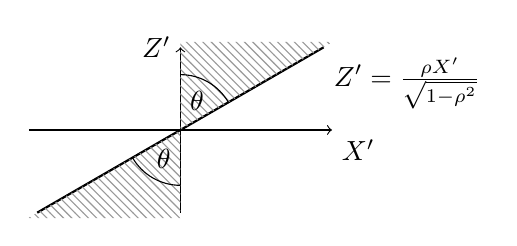
\begin{tikzpicture}[scale=0.35, background layer/.style={fill=none}]
% Define constants
\def\rhovalue{0.5}
\pgfmathsetmacro{\slope}{\rhovalue/sqrt(1-\rhovalue^2)}
\def\endX{5}
\pgfmathsetmacro{\endZ}{\slope*\endX}

% Draw axes
\draw[->] (0,-3) -- (0,3) node[left] {$Z'$};
\draw[->] (-5.5,0) -- (5.5,0) node[below right] {$X'$};

% Draw the line Z' = rho*X'/sqrt(1-rho^2) constrained within axis bounds
\pgfmathsetmacro{\leftX}{-3/\slope}  % X value where line reaches Z' = -3
\pgfmathsetmacro{\rightX}{3/\slope}  % X value where line reaches Z' = 3
\pgfmathsetmacro{\actualLeftX}{max(-5.5, \leftX)}
\pgfmathsetmacro{\actualRightX}{min(5.5, \rightX)}
\pgfmathsetmacro{\actualLeftZ}{\slope*\actualLeftX}
\pgfmathsetmacro{\actualRightZ}{\slope*\actualRightX}
\draw[thick] (\actualLeftX, \actualLeftZ) -- (\actualRightX, \actualRightZ) node[below right] {$Z' = \frac{\rho X'}{\sqrt{1-\rho^2}}$};
%\draw[thick] (\actualLeftX, \actualLeftZ) -- (\actualRightX, \actualRightZ) 
%  node[above right, xshift=-20pt, yshift=-10pt] {$Z' = \frac{\rho X'}{\sqrt{1-\rho^2}}$};


% Coordinates for angle measurement
\coordinate (O) at (0,0);
\coordinate (Zaxis) at (0,1);
\coordinate (LinePoint) at (1, \slope);
\coordinate (NegZaxis) at (0,-1);
\coordinate (NegLinePoint) at (-1, -\slope);
\coordinate (Zfar) at (0,3.2);
\coordinate (linetopfar) at (3.2/\slope, 3.2);
\coordinate (NegZfar) at (0,-3.2);
\coordinate (Neglinetopfar) at (-3.2/\slope, -3.2);

    \fill[pattern=north west lines, pattern color=black!40] 
      (O) -- (NegZfar) -- (Neglinetopfar) -- cycle;

    \fill[pattern=north west lines, pattern color=black!40] 
      (O) -- (Zfar) -- (linetopfar) -- cycle;

% Draw angle arc between Z' axis and the line
\pic[
    draw,
    angle radius=20pt,
    angle eccentricity=0.6,
    preaction={draw=white, line width=6pt},
    "$\theta$"
] {angle = LinePoint--O--Zaxis};


\pic[
    draw,
    angle radius=20pt,
    angle eccentricity=0.6,
    preaction={draw=white, line width=6pt},
    "$\theta$"
] {angle = NegLinePoint--O--NegZaxis};

\end{tikzpicture}
    \caption{$\{rX'^{2} < X'Z' \}$}
    \label{fig:proof_fig}
\end{figure}
\fi
\begin{figure}[H]
    \begin{minipage}[T]{0.48\columnwidth}
    %\vspace{0pt}
        \raggedright
        Let $r = \frac{\rho}{\sqrt{1-\rho^2}}$ and $Z' = rX' - \sqrt{1+r^{2}} Y'$ \iffalse $Z' = \frac{1}{\sqrt{1-\rho^{2}}}(\rho X' - Y')$\fi. 
        Then $\binom{X'}{Z'} \sim \mathcal{N}\left(\vect{0}, \matr{I}\right)$ and 
        $\prob{X'Y'<0}$
        \noindent$ = \prob{rX'^{2} < X'Z'} $ 
        \noindent$= 
        \mathbb{P}(\{rX' < Z' \text{ and } X' > 0\} \cup \{rX' > Z' \text{ and } X' < 0 \})$. 
        We depict this set as the shaded area in Figure \ref{fig:proof_fig}.
    \end{minipage}
    \hfill
    \begin{minipage}[T]{0.48\columnwidth}
        \centering
        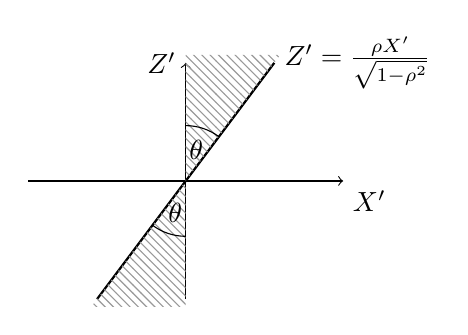
\begin{tikzpicture}[scale=0.5, background layer/.style={fill=none}]
% Define constants
\def\rhovalue{0.8}
%\pgfmathsetmacro{\slope}{\rhovalue/sqrt(1-\rhovalue^2)}
\def\slope{1.33333333333}
\def\endX{5}
\pgfmathsetmacro{\endZ}{\slope*\endX}



% Draw axes
\draw[->] (0,-3) -- (0,3) node[left] {$Z'$};
\draw[->] (-4,0) -- (4,0) node[below right] {$X'$};

% Draw the line Z' = rho*X'/sqrt(1-rho^2) constrained within axis bounds
\pgfmathsetmacro{\leftX}{-3/\slope}  % X value where line reaches Z' = -3
\pgfmathsetmacro{\rightX}{3/\slope}  % X value where line reaches Z' = 3
\pgfmathsetmacro{\actualLeftX}{max(-5.5, \leftX)}
\pgfmathsetmacro{\actualRightX}{min(5.5, \rightX)}
\pgfmathsetmacro{\actualLeftZ}{\slope*\actualLeftX}
\pgfmathsetmacro{\actualRightZ}{\slope*\actualRightX}
\draw[thick] (\actualLeftX, \actualLeftZ) -- (\actualRightX, \actualRightZ) node[right] {$Z' = \frac{\rho X'}{\sqrt{1-\rho^2}}$};
%\draw[thick] (\actualLeftX, \actualLeftZ) -- (\actualRightX, \actualRightZ) 
%  node[above right, xshift=-20pt, yshift=-10pt] {$Z' = \frac{\rho X'}{\sqrt{1-\rho^2}}$};


% Coordinates for angle measurement
\coordinate (O) at (0,0);
\coordinate (Zaxis) at (0,1);
\coordinate (LinePoint) at (1, \slope);
\coordinate (NegZaxis) at (0,-1);
\coordinate (NegLinePoint) at (-1, -\slope);
\coordinate (Zfar) at (0,3.2);
\coordinate (linetopfar) at (3.2/\slope, 3.2);
\coordinate (NegZfar) at (0,-3.2);
\coordinate (Neglinetopfar) at (-3.2/\slope, -3.2);

    \fill[pattern=north west lines, pattern color=black!40] 
      (O) -- (NegZfar) -- (Neglinetopfar) -- cycle;

    \fill[pattern=north west lines, pattern color=black!40] 
      (O) -- (Zfar) -- (linetopfar) -- cycle;


% Draw angle arc between Z' axis and the line
\pic[
    draw,
    angle radius=20pt,
    angle eccentricity=0.6,
    %preaction={draw=white, line width=6pt},
    %angle label={$\theta$}
    %label={\tikz \node[draw,fill=yellow]{2};}
    pic text=$\theta$,
] {angle = LinePoint--O--Zaxis};

\pic[
    draw,
    angle radius=20pt,
    angle eccentricity=0.6,
    %preaction={draw=white, line width=6pt},
    pic text=$\theta$,
] {angle = NegLinePoint--O--NegZaxis};

\end{tikzpicture}
        \captionof{figure}{$\{rX'^{2} < X'Z' \}$}
        \label{fig:proof_fig}
    \end{minipage}
\end{figure}

Note that $\theta = \text{arccos}(\rho)$. The distribution of $\binom{X'}{Z'}$ is rotationally invariant, so for any positive integer $m$, if $\frac{m\pi}{\theta} \in \mathbb{Z}$, we can copy and rotate the shaded area $\frac{m\pi}{\theta}$ times to cover the plane $m$ times (one covering of the plane corresponds to $\prob{X' \in \mathbb{R}, Z' \in \mathbb{R}} = 1$). Thus the shaded area is $\prob{X'Y'<0} = \frac{\theta}{\pi}$. Otherwise let $\theta_{m} = \frac{m\pi}{\left\lceil\frac{m\pi}{\theta} \right\rceil}$ and our argument applies if the shaded area were shrunk to $\theta_{m}$. Then $\theta_{m}$ tends to $\theta$ from below as $m \to \infty$ and by countable additivity of measures, $\prob{X'Y' < 0} = \lim_{m\to\infty} \frac{\theta_{m}}{\pi} = \frac{\theta}{\pi}$.
\end{proof}

We now characterise our losses for a class of linear $f$ which we interpret as a linearized GCN (see Sec \ref{sec:experimental_setup} for a specific example):
    
\begin{theorem}
\label{thm:general_class_err}
    \bs{If} the function $f$ generating the labels from the features can be written as $$f(\matr{X}) = \matr{G}\matr{X}\matr{w}$$ where $\matr{G}\in \mathbb{R}^{N \times N}$ and $\vect{w} \in \mathbb{R}^{d}$, then for a sample set $\set{S}$,
    \begin{align}
         &\text{Classification Loss}  = \sum_{i \in \set{V}} \frac{1}{\pi}\text{arccos}\left( \rho_{i}(\matr{G}) \right) \label{eq:gen_class_err}
        \\  &\text{Reconstruction Loss}  =  d \sum_{i \in \set{V}} \left(\sigma_{i}(\matr{I})\right)^{2} + \left(\nu_{i}(\matr{I})\right)^{2} - 2c_{i}(\matr{I}) \label{eq:gen_rec_err}
        %\sum_{i \in \set{V}} \frac{1}{\pi}\text{arccos}\left( \frac{\left(\matr{R}_{\set{S}}\matrsub[S,N]{\Sigma}\right)_{ii}}{\sqrt{\matr{\Sigma}_{ii}\left(\matr{R}_{\set{S}}\left(\matr{\Sigma} + n^{2}\matr{I}_{N}\right) \matr{R}_{\set{S}}^{T} \right)_{ii}}} \right)
    \end{align}
    where for any matrix $\matr{M}$, we let
    \begin{align}
        \matr{C} &= \text{Cov}(\matr{X}\vect{w}) \cdot (\sqnormvec{\vect{w}})^{-1},\\
        c_{i}(\matr{M}) &={\left(\matr{M}\matr{R}_{\set{S}}\matrsub[S,N]{C} \matr{M}^{T}\right)_{ii}}, \\
        \left(\sigma_{i}(\matr{M})\right)^{2} &= \left(\matr{M}\matr{C}\matr{M}^{T}\right)_{ii}, \\
        \left(\nu_{i}(\matr{M})\right)^{2} &= \left( \matr{M}\matr{R}_{\set{S}}\msubgen[\set{S}]{\matr{C} + \eta^{2}\matr{I}_{N}} \matr{R}_{\set{S}}^{T} \matr{M}^{T}\right)_{ii},\\
        \rho_{i}\left(\matr{M}\right) &= \frac{c_{i}(\matr{M})}{\sigma_{i}(\matr{M})\nu_{i}(\matr{M})}.
    \end{align}
\end{theorem}
\begin{proof}
    %For each node, $\expect{f(\matr{X})} = \mathbb{E}[{f(\hat{\matr{X}})}] = 0$ so 
    As $\matr{X}$ is independent to the noise and $\expect{\matr{X}}=0$,
    $\text{Cov}(f(\hat{\vect{X}})_{i}, f({\vect{X}})_{i}) = \expect{f(\hat{\vect{X}})f({\vect{X}})^{T}}_{ii} = \matr{G}\matr{R}_{\set{S}}\matrsub[S,N]{I}\expect{(\matr{X} + \eta \cdot \vect{\epsilon})\vect{w}\vect{w}^{T}\matr{X}^{T}}\matr{G}^{T}$ = $\matr{G}\matr{R}_{\set{S}}\msubgen[\set{S},\set{N}]{\text{Cov}(\matr{X}\vect{w})}\matr{G}^{T} = \sqnormvec{\vect{w}}c_{i}(\matr{G})$. Similarly, $\text{Var}(f(\matr{X})_{i}) = \sqnormvec{\vect{w}}(\sigma_{i}(\matr{G}))^{2}$ and  $\text{Var}(f(\hat{\matr{X}})_{i}) = \sqnormvec{\vect{w}}(\nu_{i}(\matr{G}))^{2}$ giving $\rho_{i}(\matr{G}) = \text{Corr}(f(\hat{\vect{X}})_{i}, f({\vect{X}})_{i})$. For classification loss, as $(f(\hat{\vect{X}})_{i}$ and $f({\vect{X}})_{i})$ are linear transformations of $\matr{X}$, they are jointly Gaussian and we can apply Lemma \ref{lemma:gaussian_sign} to get that the misclassification probability at node $i$ is $\frac{\text{arccos}(\rho_{i}(\matr{G}))}{\pi}$; sum across all nodes to get the total loss. \bs{For the Reconstruction loss, $\expect{||\matr{X} - \hat{\matr{X}}||^{2}_{F}} =  \expect{\text{tr}(\matr{X}\matr{X}^{T})} + \expect{\text{tr}(\hat{\matr{X}}\hat{\matr{X}}^{T})} - 2\expect{\text{tr}(\hat{\matr{X}}\matr{X}^{T})}  = \sum_{i \in \set{V}}d \text{Var}(\matr{X}_{i}) + d\text{Var}(\hat{\matr{X}}_{i}) - 2d\text{Cov}(\hat{\matr{X}}_{i}, \matr{X}_{i}) $. As $\expect{\matr{X}} = \expect{\hat{\matr{X}}} = 0$, this expands to (\ref{eq:gen_rec_err}). }
    
\end{proof}

% Note that classification loss is only dependent on $\matr{G}$, not $\vect{w}$.

\bs{
If we let $\matr{G}$ be a polynomial $p$ of $\tilde{\matr{A}}_{\gamma}$, then $\vect{l} = \text{sign}(p(\tilde{\matr{A}}_{\gamma})\matr{X}\matr{w})$, which corresponds to a multi-layer SGC \cite{wu2019simplifying} or a single layer polynomial-based GNN\footnote{We assume that all feature dimensions share the same polynomial filter.} like Chebnet \cite{defferrard2016convolutional}, FavardGNN \cite{guo2023Favard}, JacobiNet \cite{guo2023manipulating} or BernNet \cite{he2021bernnet}. Then the classification loss in Theorem \ref{thm:general_class_err} is the difference in output when applying the GNN to the full data $\matr{X}$ versus to the reconstructed data $\hat{\matr{X}}$. 
Note that in the case where the columns of $\matr{X}$ are independent, $\matr{C} = \matr{\Sigma}$, and therefore for SGC the classification loss does not depend on the weights, only on the number of layers.
}

%We can use \bs{Theorem \ref{thm:general_class_err}} to calculate the classification \bs{loss} for an $r$-layer \bs{linearized} GCN without bias, setting $\matr{G} = (\tilde{\matr{A}}_{\gamma})^{r}$ and $\vect{w} = \prod \matr{W}_{i}$. The classification \bs{loss then} does not depend on the weights \bs{$\vect{w}$} -- if our linearized GCN is an accurate representation of the true function, then the classification \bs{loss} is not dependent on its weights, only its structure \bs{$\matr{G}$} (i.e. the number of layers). 

 To interpret Theorem \ref{thm:general_class_err}, we consider any $\matr{G}$ and LS reconstruction of a noise-free $k$-bandlimited signal; specifically $\matr{\Sigma} = \projbl$. In this case, $\sqrt{c_{i}(\matr{G})} = \nu_{i}(\matr{G})$ and the {\text{classification loss}} is $\sum_{i \in \set{V}} \frac{1}{\pi}\arccos{\left(\sqrt{\frac{c_{i}}{\sigma_{i}}}\right)}$ where $0 \leq \frac{c_{i}}{\sigma_{i}} \leq 1$. Thus, we expect the behaviour of classification \bs{loss} as it changes with sample size to look similar to $x \to \arccos{\left(\sqrt{x}\right)}$.

%We briefly contrast our result to the literature on moderation. Mackay \cite{mackay1992evidence} noted that uncertainty -- lack of information -- over the weights causes a sigmoid shaped posterior probability. We note that in the above case, lack of information about the data causes a sigmoid shaped error as sample size varies.


\subsection{Relationship between Reconstruction and Classification Loss}
We now relate the reconstruction and classification losses via the error in reconstructing the output of $f$:

\begin{corollary}
\label{corr:relationship}
    Assume the setting and definitions of Theorem \ref{thm:general_class_err}. 
    Define the normalized output error at node $i$ as 
    \begin{equation}
    \text{Error}_{out, i} = \left(\sqnormvec{\vect{w}}\right)^{-1}{\expect{||(f(\matr{X}))_i - (f(\hat{\matr{X}}))_i||^{2}_{2}}}. 
    \end{equation}
%Then if for some $r \geq 0, \gamma \geq 0$, $\matr{G} =  \tilde{\matr{A}}_{\gamma}^{r}$,
Let $||\matr{G}||$ be the spectral norm of $\matr{G}$, then
\begin{equation}
\label{eq:bound_final_layer}
\sum_{i \in \set{V}} \text{Error}_{out,i} \leq ||\matr{G}||^{2} \cdot \text{Reconstruction Loss}
\end{equation}
and for every node $i$, the following is always a valid triangle.
\begin{figure}[H]
    \centering
    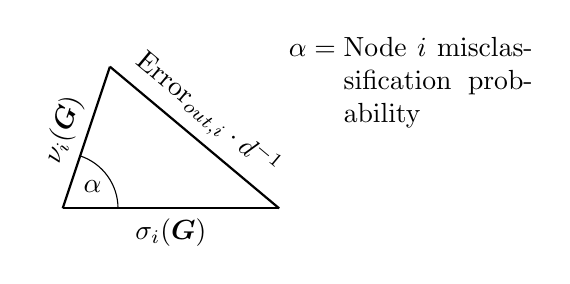
\begin{tikzpicture}[scale=0.5]
    \def\slope{3}
    \def\xA{5.5}
    \def\yA{0}
    \def\xB{1.2}
    \def\yB{\xB * \slope}
    \pgfmathsetmacro{\etaValue}{atan(\slope)}
    
    %\pgfmathsetmacro{\slope}{\rhovalue/sqrt(1-\rhovalue^2)}
    % Define the vertices of the triangle
    \coordinate (O) at (0,0);
    \coordinate (A) at (\xA,\yA);
    \coordinate (B) at (\xB,\yB);
    
    \pgfmathsetmacro{\otherRot}{atan2(\yA - \yB, \xA - \xB}


    
    % Draw the triangle
    %\draw[thick] (O) -- (A) -- (B) -- cycle;
    
    \draw[thick] (O)--(A)  node[midway, below] {$\sigma_{i}(\matr{G})$}; %{$\sqrt{\text{Var}(f(\matr{X}))_i}$};
    
    \draw[thick] (O)--(B)  node[midway, above, rotate=\etaValue] {$\nu_{i}(\matr{G})$}; %{$\sqrt{\text{Var}(f(\hat{\matr{X}}))_i}$};
    
    \draw[thick] (A)--(B)  node[midway, above, rotate=\otherRot, align=center] {
    $\text{Error}_{out,i} \cdot d^{-1} $
    };

    %\draw[thick] (A)--(B)  node[midway, above, rotate=\otherRot, align=center, text width=100pt] {Final layer reconstruction error at node $i$}; %{$\sqrt{\expect{||(f(\matr{X}))_i - (f(\hat{\matr{X}}))_i||^2}}$} ;
    % Label the vertices
    \iffalse
    \node[below left] at (O) {$0$};
    \node[below right] at (A) {$f(\matr{X})_i$};
    \node[above] at (B) {$f(\hat{\matr{X}})_i$};
    \fi
    
    
\pic[
    draw,
    angle radius=20pt,
    angle eccentricity=1,
    preaction={draw=white, line width=6pt},
    %"Classification\\Error",%"${\eta}$"
] {angle = A--O--B};
\node[right, xshift=4pt, yshift=8pt, text width=50pt] at (O) {$\alpha$};%{Node $i$ Classification Error };
%\node[right, rotate=\etaValue/2, xshift=20pt, yshift=0pt, text width=50pt] at (O) {Node $i$ Misclassification Probability};%{Node $i$ Classification Error };

\node[below, right] at (\xA,\yB-0.4) {$\alpha = \parbox[t][][t]{2.4cm}{Node $i$ misclassification probability }$};
%\node[above, text width=3cm] at (\xA,-2) {Node $i$ Misclassification Probability};



    % Add small circles at vertices for clarity
    \iffalse
    \fill (O) circle (1pt);
    \fill (A) circle (1pt);
    \fill (B) circle (1pt);
    \fi
\end{tikzpicture}
    \caption{Relationship between misclassification probability \iffalse Classification Loss \fi (angle) and normalized output error at node $i$}
    \label{fig:class_rec_rel_fig}
\end{figure}

\end{corollary}
\begin{proof}
    We first prove \eqref{eq:bound_final_layer}. %Write the spectral norm of a matrix $\matr{M}$ as  $||\matr{M}||$. By Gershgorin's Circle Theorem, $||\tilde{\matr{A}}|| \leq 1$; thus by \cite[Theorem 1]{wu2019simplifying}, $||\tilde{\matr{A}}_{\gamma}|| \leq 1$. Therefore $||\matr{G}|| \leq 1$. 
    By linearity of $f$, $(f(\matr{X}))_i - (f(\hat{\matr{X}}))_i = (\matr{G}(\matr{X} - \hat{\matr{X}})\vect{w})_{i}$. Then  $\sum_{i \in \set{V}} ||f(\matr{X})_{i} - f(\hat{\matr{X}})_{i} ||_{2}^{2} = ||\matr{G}(\matr{X} - \hat{\matr{X}})\vect{w}||_{2}^{2} \leq ||\matr{G}||^{2}\cdot ||(\matr{X} - \hat{\matr{X}})\vect{w}||_{2}^{2} \leq ||\matr{G}||^{2} \cdot (\matr{X} - \hat{\matr{X}})||_{F}^{2} \cdot ||\vect{w}||_{2}^{2}$ where the last inequality is because $||\cdot||_{2} = ||\cdot||_{F}$ for vectors and from sub-multiplicativity of $||\cdot||_{F}$. Taking expectations on both sides gives $ \sqnormvec{\vect{w}} \cdot \sum_{i \in \set{V}} \text{Error}_{out,i} \leq ||\matr{G}||^{2} \cdot  \text{Reconstruction Loss} \cdot ||\vect{w}||_{2}^{2}$. 

    Secondly, we prove Fig. \ref{fig:class_rec_rel_fig} forms a valid triangle. Through the same expansion and independence arguments as in the proof of Theorem \ref{thm:general_class_err}, $\text{Error}_{out,i} = d\cdot \left((\sigma_{i}(\matr{G}))^{2} + (\nu_{i}(\matr{G}))^{2} - 2\rho_{i}(\matr{G}) \right)$. As $\rho_{i}(\matr{G})$ is the probability of misclassification of node $i$ (see the proof of Theorem \ref{thm:general_class_err}), the sides and angle of Fig. \ref{fig:class_rec_rel_fig} obey the law of cosines and thus form a valid triangle.
\end{proof}


For SGCs, $||\matr{G}|| \leq 1$ (as $||\tilde{\matr{A}}|| \leq 1$ by Gershgorin's Disc Theorem \cite{horn-and-johnson}, so $\forall \gamma\geq 0:||\tilde{\matr{A}}_{\gamma}|| \leq 1$ by \cite[Theorem 1]{wu2019simplifying} and therefore $||\tilde{\matr{A}}_{\gamma}^{r}|| \leq 1$ for all $r \geq 1$). Therefore, by \eqref{eq:bound_final_layer}, the sum of the per-node normalized output errors (which are directly related to the per-node misclassification probabilities, as shown in Fig. \ref{fig:class_rec_rel_fig}) is upper bounded by the reconstruction loss.
\iffalse
Figure \ref{fig:class_rec_rel_fig} shows the relationship between error of reconstruction of the final layer output (i.e., ${\expect{||(f(\matr{X}))_i - (f(\hat{\matr{X}}))_i||^{2}_{2}}}$) and per-node misclassification probability (i.e., per-node classification loss), namely that they form a triangle, which follows from Theorem \ref{thm:general_class_err} and the law of cosines:

\begin{figure}[H]
    \centering
    
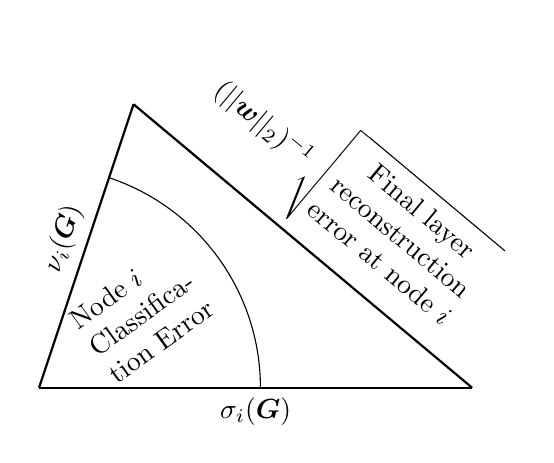
\begin{tikzpicture}[scale=1]
    \def\slope{3}
    \def\xA{5.5}
    \def\yA{0}
    \def\xB{1.2}
    \def\yB{\xB * \slope}
    \pgfmathsetmacro{\etaValue}{atan(\slope)}
    
    %\pgfmathsetmacro{\slope}{\rhovalue/sqrt(1-\rhovalue^2)}
    % Define the vertices of the triangle
    \coordinate (O) at (0,0);
    \coordinate (A) at (\xA,\yA);
    \coordinate (B) at (\xB,\yB);
    
    \pgfmathsetmacro{\otherRot}{atan2(\yA - \yB, \xA - \xB}
    
    % Draw the triangle
    %\draw[thick] (O) -- (A) -- (B) -- cycle;
    
    \draw[thick] (O)--(A)  node[midway, below] {$\sigma_{i}(\matr{G})$}; %{$\sqrt{\text{Var}(f(\matr{X}))_i}$};
    
    \draw[thick] (O)--(B)  node[midway, above, rotate=\etaValue] {$\nu_{i}(\matr{G})$}; %{$\sqrt{\text{Var}(f(\hat{\matr{X}}))_i}$};
    
    \draw[thick] (A)--(B)  node[midway, above, rotate=\otherRot, align=center] {
        $(||\vect{w}||_{2})^{-1}\sqrt{\expect{\begin{tabular}{@{}c@{}}
            Final layer \\ reconstruction \\
            error at node $i$
        \end{tabular}}}$
    };

    %\draw[thick] (A)--(B)  node[midway, above, rotate=\otherRot, align=center, text width=100pt] {Final layer reconstruction error at node $i$}; %{$\sqrt{\expect{||(f(\matr{X}))_i - (f(\hat{\matr{X}}))_i||^2}}$} ;
    % Label the vertices
    \iffalse
    \node[below left] at (O) {$0$};
    \node[below right] at (A) {$f(\matr{X})_i$};
    \node[above] at (B) {$f(\hat{\matr{X}})_i$};
    \fi
    
    
\pic[
    draw,
    angle radius=80pt,
    angle eccentricity=1,
    preaction={draw=white, line width=6pt},
    %"Classification\\Error",%"${\eta}$"
] {angle = A--O--B};
\node[right, rotate=\etaValue/2, xshift=20pt, yshift=0pt, text width=50pt] at (O) {Node $i$ Classification Error };


    % Add small circles at vertices for clarity
    \iffalse
    \fill (O) circle (1pt);
    \fill (A) circle (1pt);
    \fill (B) circle (1pt);
    \fi
\end{tikzpicture}
    \caption{Relationship between \bs{Misclassification Probability} \iffalse Classification \bs{Loss} \fi (angle) and \bs{Final Layer} Reconstruction error ($\sqnormvec{\vect{w}} \times \text{side length}^{2}$) at node $i$}
    \label{fig:class_rec_rel_fig}
\end{figure}
We also note that $\sigma_{i}(\matr{G})$ (respectively $\nu_{i}(\matr{G})$) is the standard deviation of the true (respectively reconstructed) final layer output (before the sign function) at node $i$.
\bs{
We now relate final layer reconstruction error to the reconstruction loss (the error in reconstructing the features) -- as $f = \matr{G}{\matr{X}}\vect{w}$ is linear, and because for all matrices $\matr{X},\matr{Y}$, $||\matr{X}\matr{Y}||_{F} \leq ||\matr{X}|| \cdot ||\matr{Y}||_{F}$ (apply H\"older's inequality \cite[Sec III]{ball2002sharp} with $p=\infty, q=r=2$),  we have
\begin{equation}
\label{eq:bound_final_layer}
(\sqnormvec{\vect{w}})^{-1} {\expect{||(f(\matr{X})) - (f(\hat{\matr{X}}))||^{2}_{F}}} \leq ||\matr{G}||^{2} \cdot \expect{||\matr{X} - \hat{\matr{X}}||_{F}^{2}}
\end{equation}
where $||\matr{G}||$ is the spectral norm of $\matr{G}$. The left of \eqref{eq:bound_final_layer} is the sum of the final layer reconstruction error across all nodes, divided by the squared-norm of the weight matrix $\vect{w}$ of $f$. This is upper bounded by the reconstruction loss times the spectral norm of $\matr{G}$. In the case of a SGC on an undirected graph, i.e., where $\matr{G}$ is a power of a normalized symmetric adjacency matrix, $||\matr{G}|| \leq 1$ (By Gershgorin's Circle Theorem, any non-loopy symmetric degree-normalized adjacency matrix has spectral radius 1; use \cite[Theorem 1]{wu2019simplifying} to extend to the loopy case).
}
%We see that $\rho_{i}(\matr{G})$ is the correlation at node $i$ between the true classification and the reconstructed classification. 
\fi

%Next we consider any reconstruction method, in the case that $\matr{G}=\matr{I}$. We see that on a node-by-node basis, both losses are decreasing in $c_{i}$ and increasing in $\sigma_{i}$ and $\nu_{i}$. We therefore expect both objectives to work well for each other but not optimally.

\bs{
\subsection{Sampling for Classification}
\label{sec:optimal_sampling_design}
We use Theorem \ref{thm:general_class_err} to design a sampling scheme specifically for classification, minimising mean classification loss rather than the common mean reconstruction loss objective \cite{wang2018optimal,wang2019low,sripathmanathan2024impact, mfn}. We propose greedily choosing $\set{S}$ to optimize \eqref{eq:gen_class_err} from Theorem \ref{thm:general_class_err}. %and compare it to random and A-optimal sampling under both reconstruction and classification.
}

\section{Empirical Results}
%We now validate our theoretical results by empirical experiments \bs{and compare the performance of our classification-optimal sampling scheme to other sample schemes designed with reconstruction in mind.} %and  We also apply our theoretical results to propose an optimal sampling scheme for classification under our setup, and compare its performance to other optimal sampling schemes aiming for reconstruction only.
\iffalse
BA:
[SGC, Simple] 
x
[LS,
%(GLR),
Feat Prop]

%[noiseless, noisy] x 
noisy vs noiseless for LS
[BA, SBM] - 1 figure SBM

%[bandlimited signal, L+ signal]
For each comparison each fig should have the same x \& y

classic setting :LS x bandlimited signal -- best performance for our sample selection scheme

%SGC: BL (1 layer: sign((AXW2)W2) )
%SGC: L+ (2 layersL
\fi
\subsection{Experimental Setup}
\label{sec:experimental_setup}
%We first present the setup of our experiments. All experiments are with regards to the symmetrically normalized Laplacian and its eigenbasis.

\subsubsection{Synthetic Graph Generation}
We generate 32 graphs with $N=500$ nodes from each of the following models:
\begin{itemize}
    \item Barab\'asi-Albert (BA) with a preferential attachment to 3 vertices at each step of construction;
    \item Stochastic Blockmodel (SBM) with intra- and inter- cluster edge probabilities of 0.7 and 0.1, respectively.
\end{itemize}

\iffalse
\subsubsection{Choice of $f$}
We consider two types of classification function. In the `simple' case, we consider $d=1$ and $f(x) = x$, so the label is the sign of the true feature. In the `sgc' case, we consider a random linearized GCN with added self-loops as a model for $f$. We choose our architecture to mimic the strong baselines in \cite{luo2024classic}. Specifically:
\begin{equation}
    f_{\text{sgc}, r}(\matr{X}) = (\matr{I} + \tilde{\matr{A}})^{r}\matr{X}\prod_{i=1}^{r+1}\matr{W}_{i}.
\end{equation}
Our first layer has $\matr{W}_{1}\in\mathbb{R}^{64\times 32}$, any intermediate layer has $\matr{W}_{i} \in \mathbb{R}^{32 \times 32}$ and our final readout layer has $\matr{W}_{r+1} \in \mathbb{R}^{32 \times 1}$. We populate $\matr{W}_{i}$ via Glorot initialization \cite{glorot2010understanding}. We choose $r=1$ to avoid label oversmoothing.
\fi

\subsubsection{Synthetic Signal Generation}
\bs{We draw features $\matr{X}$ as described in Section \ref{sec:problem_setting} with $\matr{\Sigma} = \projbl$, i.i.d. columns, bandwidth $k = \frac{N}{10}$ and noise variance $\eta^{2}=10^{-3}$ so the SNR is $20dB$, like in \cite{bai2020fast}. }
%We consider signals drawn from $\mathcal{N}(\vect{0},\projbl)$ (i.e. $\matr{\Sigma} = \projbl$) with bandwidth $k = \frac{N}{10}$. We consider both noiseless signals and signals with $\mathcal{N}(\vect{0}, 10^{-3} \matr{I}_{N})$ noise added ($n=10^{-1.5}$) so the SNR is 20dB, like in \cite{bai2020fast}. \bs{We draw a single feature matrix $\matr{X}\in\mathbb{R}^{500 \times 64}$ per graph.}
%We draw 200 signals per graph instantiation in the `simple' $f$ case (i.e. $32 \times 200$ classification tasks per graph model). We draw one task per graph in the `sgc' $f$ case (corresponding to $\matr{X} \in \mathbb{R}^{500 \times 64}$).

\subsubsection{Choice of $f$}
\bs{For each graph, we construct $f$ as a linearized GCN with randomly initialized weights and added self-loops ($\gamma=1)$. We choose our architecture to mimic the strong baselines in \cite{luo2024classic}, but keep to a single convolutional layer to minimise oversmoothing.
Specifically, we set
\begin{equation}
 f(\matr{X}) = \tilde{\matr{A}}_{1}\matr{X}\left(\matr{W}_{1}\matr{W}_{2} \right)
\end{equation}
 where $\matr{W}_{1} \in \mathbb{R}^{64 \times 32}$, $\matr{W}_{2} \in \mathbb{R}^{32 \times 1}$ are both populated via Glorot initialization \cite{glorot2010understanding}.}

\subsubsection{Real-world Datasets}
We consider an FMRI dataset with nodes corresponding to brain regions and 292 graph signals corresponding to blood oxygen levels \cite{zhi2023gaussian, sripathmanathan2024impact}, subsampling a connected graph with $N=367$ nodes using neighbourhood sampling \cite{hamilton2017inductive}. We do not bandlimit the \bs{given} signals. We construct a classification task by subtracting the mean from all signals and taking the sign as node class labels, representing high or low blood oxygen levels.

%We use optimal sampling assuming an SNR of 20dB (i.e., $n=10^{-1.5}$) and reconstruct with a bandlimit of $\lfloor \frac{N}{10} \rfloor$.

\subsubsection{Sample Set Selection}
We consider three sampling methods:
\begin{itemize}
    \item Random sampling;
    \item Greedy sampling optimizing classification \bs{loss} \eqref{eq:gen_class_err}, which is described in Sec \ref{sec:optimal_sampling_design};
    \item Greedy sampling optimizing reconstruction \bs{loss} \eqref{eq:gen_rec_err}. For LS, this is the same as optimizing for the frequently used A-optimal objective for reconstruction \cite{wang2018optimal, wang2019low, sripathmanathan2024impact, mfn}.
\end{itemize}

%Under LS reconstruction, \iffalse and $\matr{\Sigma}=\projbl$\fi multiple nodes are frequently tied in reconstruction error. In this case, we also optimize for noise sensitivity, and this sample choice corresponds to A-optimal sampling \cite{wang2018optimal}.

%\bs{In our setup, greedily optimizing reconstruction loss is the same as greedily optimizing the frequently used A-optimal objective for reconstruction \cite{wang2018optimal, wang2019low, sripathmanathan2024impact, mfn}.}

\bs{To sample on real world data, we need to compute losses for our sampling to optimize. This requires making assumptions about the noise level and distribution of the features. For the FMRI dataset, we assume the features are i.i.d. $\mathcal{N}(\vect{0},\projbl)$ with $k = \lfloor \frac{N}{10}\rfloor$ and that the SNR is $20dB$ (i.e., $\eta^{2}=10^{-3}$). }


\setlength{\belowcaptionskip}{-3pt}
%\captionsetup[subfigure]{aboveskip=-1pt,belowskip=-4pt}
\captionsetup[subfigure]{aboveskip=-1pt,belowskip=-2.5pt}
%\setlength{\abovecaptionskip}{-3pt}
%\setlength{\aftercaptionskip}{-0.3cm}
%\setlength{\intextsep}{0pt plus 2pt}
\iffalse
%%% Simple, LS, BA, Noiseless
\begin{figure*}%
    \centering
    \begin{subfigure}[T]{0.5\columnwidth}
    \resizebox{\width}{0.62\columnwidth}{
    \includegraphics[width=\columnwidth]{figures/proj2/plots/simple/BA_bl_LS_0_noise_500_nodes_class_vs_rec.png}}
    \caption{Loss Comparison \\}
    \label{subsubfig:BA_noiseless_simple_LS_comp}
    \end{subfigure}
    \hfill
    \begin{subfigure}[T]{0.5\columnwidth}
    \resizebox{\width}{0.62\columnwidth}{
    \includegraphics[width=\columnwidth]{figures/proj2/plots/simple/BA_bl_LS_0_noise_500_nodes_recon.png}}
    \caption{Reconstruction Loss}%
    \label{subsubfig:BA_noiseless_simple_LS_rec}
    \end{subfigure}
    \hfill%
    \begin{subfigure}[T]{0.5\columnwidth}
    \resizebox{\width}{0.62\columnwidth}{
    \includegraphics[width=\columnwidth]{figures/proj2/plots/simple/BA_bl_LS_0_noise_500_nodes_classif.png}}
    \caption{Class. Loss (Analytic)}
    \label{subsubfig:BA_noiseless_simple_LS_class_anal}
    \end{subfigure}%
    \hfill
    \begin{subfigure}[T]{0.5\columnwidth}
    \resizebox{\width}{0.62\columnwidth}{
    \includegraphics[width=\columnwidth]{figures/proj2/plots/simple/BA_bl_LS_0_noise_500_nodes_class_empiric.png}}
    \caption{Class. Loss (Empirical)}%
    \label{subsubfig:BA_noiseless_simple_LS_class_emp}
    \end{subfigure}%
    \caption{LS Reconstruction, BA graph model, noiseless}
\label{subfig:BA_noiseless_simple_LS}
\end{figure*}
\fi
%%% SGC, LS, BA, Noiseless
\begin{figure*}%
    \centering
    \iffalse
    \begin{subfigure}[T]{0.5\columnwidth}
    \resizebox{\width}{0.62\columnwidth}{
    \includegraphics[width=\columnwidth, trim={1000cm 2cm 0 0}, clip]{figures/proj2/plots/sgc-paper/BA_bl_LS_0_noise_500_nodes_1_layers_class_vs_rec.png}}
    \caption{Loss Comparison \\}
    \label{subsubfig:BA_noiseless_sgc_LS_comp}
    \end{subfigure}
    \hfill
    \fi
    \begin{subfigure}[T]{0.5\columnwidth}
    \resizebox{\width}{0.62\columnwidth}{
    \includegraphics[width=\columnwidth]{figures/proj2/plots/sgc-paper/BA_bl_LS_0_noise_500_nodes_1_layers_recon.png}}
    \caption{Reconstruction Loss}%
    \label{subsubfig:BA_noiseless_sgc_LS_rec}
    \end{subfigure}
    %\hfill%
    \begin{subfigure}[T]{0.5\columnwidth}
    \resizebox{\width}{0.62\columnwidth}{
    \includegraphics[width=\columnwidth]{figures/proj2/plots/sgc-paper/BA_bl_LS_0_noise_500_nodes_1_layers_classif.png}}
    \caption{Class. Loss (Analytic)}
    \label{subsubfig:BA_noiseless_sgc_LS_class_anal}
    \end{subfigure}%
    %\hfill
    \begin{subfigure}[T]{0.5\columnwidth}
    \resizebox{\width}{0.62\columnwidth}{
    \includegraphics[width=\columnwidth]{figures/proj2/plots/sgc-paper/BA_bl_LS_0_noise_500_nodes_1_layers_class_empiric.png}}
    \caption{Class. Loss (Empirical)}%
    \label{subsubfig:BA_noiseless_sgc_LS_class_emp}
    \end{subfigure}%
    \caption{LS Reconstruction, BA graph model, noiseless}
    \vspace{-0.19cm}
\label{subfig:BA_noiseless_sgc_LS}
\end{figure*}

%%% SGC, feat_prop, BA, Noiseless
\begin{figure*}%
    \centering
    \iffalse
    \begin{subfigure}[T]{0.5\columnwidth}
    \resizebox{\width}{0.62\columnwidth}{
    \includegraphics[width=\columnwidth]{figures/proj2/plots/sgc-paper/BA_bl_feat_prop_0_noise_200_nodes_1_layers_class_vs_rec.png}}
    \caption{Loss Comparison \\}
    \label{subsubfig:BA_noiseless_sgc_feat_prop_comp}
    \end{subfigure}
    \hfill
    \fi
    \begin{subfigure}[T]{0.5\columnwidth}
    \resizebox{\width}{0.62\columnwidth}{
    \includegraphics[width=\columnwidth]{figures/proj2/plots/sgc-paper/BA_bl_feat_prop_0_noise_500_nodes_1_layers_recon.png}}
    \caption{Reconstruction Loss}%
    \label{subsubfig:BA_noiseless_sgc_feat_prop_rec}
    \end{subfigure}
    %\hfill%
    \begin{subfigure}[T]{0.5\columnwidth}
    \resizebox{\width}{0.62\columnwidth}{
    \includegraphics[width=\columnwidth]{figures/proj2/plots/sgc-paper/BA_bl_feat_prop_0_noise_500_nodes_1_layers_classif.png}}
    \caption{Class. Loss (Analytic)}
    \label{subsubfig:BA_noiseless_sgc_feat_prop_class_anal}
    \end{subfigure}%
    %\hfill
    \begin{subfigure}[T]{0.5\columnwidth}
    \resizebox{\width}{0.62\columnwidth}{
    \includegraphics[width=\columnwidth]{figures/proj2/plots/sgc-paper/BA_bl_feat_prop_0_noise_500_nodes_1_layers_class_empiric.png}}
    \caption{Class. Loss (Empirical)}%
    \label{subsubfig:BA_noiseless_sgc_feat_prop_class_emp}
    \end{subfigure}%
    \caption{FP Reconstruction, BA graph model, noiseless}
    \vspace{-0.19cm}
\label{subfig:BA_noiseless_sgc_feat_prop}
\end{figure*}

%%% SGC, LS, BA, Noisy
\begin{figure*}%

    \centering
    \iffalse
    \begin{subfigure}[T]{0.5\columnwidth}
    \resizebox{\width}{0.62\columnwidth}{
    \includegraphics[width=\columnwidth]{figures/proj2/plots/sgc-paper/BA_bl_LS_0.03162277660168379_noise_500_nodes_1_layers_class_vs_rec.png}}
    \caption{Loss Comparison}
    \label{subsubfig:BA_noisy_sgc_LS_comp}
    \end{subfigure}
    \hfill
    \fi
    \begin{subfigure}[T]{0.5\columnwidth}
    \resizebox{\width}{0.62\columnwidth}{
    \includegraphics[width=\columnwidth]{figures/proj2/plots/sgc-paper/BA_bl_LS_0.03162277660168379_noise_500_nodes_1_layers_recon.png}}
    \caption{Reconstruction Loss}%
    \label{subsubfig:BA_noisy_sgc_LS_rec}
    \end{subfigure}
    %\hfill%
    \begin{subfigure}[T]{0.5\columnwidth}
    \resizebox{\width}{0.62\columnwidth}{
    \includegraphics[width=\columnwidth]{figures/proj2/plots/sgc-paper/BA_bl_LS_0.03162277660168379_noise_500_nodes_1_layers_classif.png}}
    \caption{Class. Loss (Analytic)}
    \label{subsubfig:BA_noisy_sgc_LS_class_anal}
    \end{subfigure}%
    %\hfill
    \begin{subfigure}[T]{0.5\columnwidth}
    \resizebox{\width}{0.62\columnwidth}{
    \includegraphics[width=\columnwidth]{figures/proj2/plots/sgc-paper/BA_bl_LS_0.03162277660168379_noise_500_nodes_1_layers_class_empiric.png}}
    \caption{Class. Loss (Empirical)}%
    \label{subsubfig:BA_noisy_sgc_LS_class_emp}
    \end{subfigure}%
    \caption{LS Reconstruction, BA graph model, Noisy ($20dB$ signal)}
    \vspace{-0.19cm}
\label{subfig:BA_noisy_vs_noisy_sgc_LS}
\end{figure*}


%%% SGC, LS, SBM, Noiseless
\begin{figure*}[h]%
    \centering
    \iffalse
    \begin{subfigure}[T]{0.5\columnwidth}
    \resizebox{\width}{0.62\columnwidth}{
    \includegraphics[width=\columnwidth]{figures/proj2/plots/sgc-paper/SBM_bl_LS_0_noise_500_nodes_1_layers_class_vs_rec.png}}
    \caption{Loss Comparison \\}
    \label{subsubfig:SBM_noiseless_sgc_LS_comp}
    \end{subfigure}
    \fi
    %\hfill
    \begin{subfigure}[T]{0.5\columnwidth}
    \resizebox{\width}{0.62\columnwidth}{
    \includegraphics[width=\columnwidth]{figures/proj2/plots/sgc-paper/SBM_bl_LS_0_noise_500_nodes_1_layers_recon.png}}
    \caption{Reconstruction Loss}%
    \label{subsubfig:SBM_noiseless_sgc_LS_rec}
    \end{subfigure}
    %\hfill%
    \begin{subfigure}[T]{0.5\columnwidth}
    \resizebox{\width}{0.62\columnwidth}{
    \includegraphics[width=\columnwidth]{figures/proj2/plots/sgc-paper/SBM_bl_LS_0_noise_500_nodes_1_layers_classif.png}}
    \caption{Class. Loss (Analytic)}
    \label{subsubfig:SBM_noiseless_sgc_LS_class_anal}
    \end{subfigure}%
    %\hfill
    \begin{subfigure}[T]{0.5\columnwidth}
    \resizebox{\width}{0.62\columnwidth}{
    \includegraphics[width=\columnwidth]{figures/proj2/plots/sgc-paper/SBM_bl_LS_0_noise_500_nodes_1_layers_class_empiric.png}}
    \caption{Class. Loss (Empirical)}%
    \label{subsubfig:SBM_noiseless_sgc_LS_class_emp}
    \end{subfigure}%
    \caption{LS Reconstruction, SBM graph model, noiseless}
    \vspace{-0.19cm}
\label{subfig:SBM_noiseless_sgc_LS}
\end{figure*}


\iffalse
%%% NEW FIG


\begin{figure*}
    \renewcommand{\arraystretch}{0}
  \centering
  \begin{tabular}{p{4pt} >{\centering\arraybackslash}p{0.29\columnwidth}@{\quad}ccc}
    & Setting & \hspace{20pt}(i) Reconstruction Loss & \hspace{13pt} (ii) Class. Loss (Analytic) & \hspace{13pt} (iii) Class. Loss (Empirical) \\ 
    \raisebox{0.26\columnwidth}[0pt][0pt]{(a)} & \raisebox{0.26\columnwidth}[0pt][0pt]{\parbox[t]{0.31\columnwidth}{\raggedright  LS Reconstruction, \\ BA graph model, \\ Noiseless}} & \includegraphics[width=0.5\columnwidth,height=0.3\columnwidth,keepaspectratio=false]{figures/proj2/plots/sgc-paper/BA_bl_LS_0_noise_500_nodes_1_layers_recon.png}\fixedlabel{fig:syn:LS_BA_Noiseless_rec}{a.i.} 
      & \includegraphics[width=0.5\columnwidth,height=0.3\columnwidth,keepaspectratio=false]{figures/proj2/plots/sgc-paper/BA_bl_LS_0_noise_500_nodes_1_layers_classif.png} \fixedlabel{fig:syn:LS_BA_Noiseless_class_anal}{a.ii.} 
      & \includegraphics[width=0.5\columnwidth,height=0.3\columnwidth,keepaspectratio=false]{figures/proj2/plots/sgc-paper/BA_bl_LS_0_noise_500_nodes_1_layers_class_empiric.png} \fixedlabel{fig:syn:LS_BA_Noiseless_class_emp}{a.iii.}
      \\
    \raisebox{0.26\columnwidth}[0pt][0pt]{(b)} & \raisebox{0.26\columnwidth}[0pt][0pt]{\parbox[t]{0.31\columnwidth}{\raggedright FP Reconstruction, \\ BA graph model, \\ Noiseless}} & \includegraphics[width=0.5\columnwidth,height=0.3\columnwidth,keepaspectratio=false]{figures/proj2/plots/sgc-paper/BA_bl_feat_prop_0_noise_200_nodes_1_layers_recon.png}\fixedlabel{fig:syn:FP_BA_Noiseless_rec}{b.i.} 
      & \includegraphics[width=0.5\columnwidth,height=0.3\columnwidth,keepaspectratio=false]{figures/proj2/plots/sgc-paper/BA_bl_feat_prop_0_noise_200_nodes_1_layers_classif.png}\fixedlabel{fig:syn:FP_BA_Noiseless_class_anal}{b.ii.}
      & \includegraphics[width=0.5\columnwidth,height=0.3\columnwidth,keepaspectratio=false]{figures/proj2/plots/sgc-paper/BA_bl_feat_prop_0_noise_200_nodes_1_layers_class_empiric.png}\fixedlabel{fig:syn:FP_BA_Noiseless_class_emp}{b.iii.} 
      \\
    \raisebox{0.26\columnwidth}[0pt][0pt]{(c) } & \raisebox{0.26\columnwidth}[0pt][0pt]{\parbox[t]{0.31\columnwidth}{\raggedright LS Reconstruction, \\ BA graph model, \\ Noisy ($20dB$ signal)}} & \includegraphics[width=0.5\columnwidth,height=0.3\columnwidth,keepaspectratio=false]{figures/proj2/plots/sgc-paper/BA_bl_LS_0.03162277660168379_noise_500_nodes_1_layers_recon.png} \fixedlabel{fig:syn:LS_BA_Noisy_rec}{c.i.} 
      & \includegraphics[width=0.5\columnwidth,height=0.3\columnwidth,keepaspectratio=false]{figures/proj2/plots/sgc-paper/BA_bl_LS_0.03162277660168379_noise_500_nodes_1_layers_classif.png} \fixedlabel{fig:syn:LS_BA_Noisy_class_anal}{c.ii.}
      & \includegraphics[width=0.5\columnwidth,height=0.3\columnwidth,keepaspectratio=false]{figures/proj2/plots/sgc-paper/BA_bl_LS_0.03162277660168379_noise_500_nodes_1_layers_class_empiric.png} \fixedlabel{fig:syn:LS_BA_Noisy_class_emp}{c.iii.}
      \\
    \raisebox{0.26\columnwidth}[0pt][0pt]{(d)} & \raisebox{0.26\columnwidth}[0pt][0pt]{\parbox[t]{0.31\columnwidth}{\raggedright LS Reconstruction, \\ SBM graph model, \\ Noiseless}} & \includegraphics[width=0.5\columnwidth,height=0.3\columnwidth,keepaspectratio=false]{figures/proj2/plots/sgc-paper/SBM_bl_LS_0_noise_500_nodes_1_layers_recon.png}\fixedlabel{fig:syn:LS_SBM_Noiseless_rec}{d.i.} 
      & \includegraphics[width=0.5\columnwidth,height=0.3\columnwidth,keepaspectratio=false]{figures/proj2/plots/sgc-paper/SBM_bl_LS_0_noise_500_nodes_1_layers_classif.png}\fixedlabel{fig:syn:LS_SBM_Noiseless_class_anal}{d.ii.}
      & \includegraphics[width=0.5\columnwidth,height=0.3\columnwidth,keepaspectratio=false]{figures/proj2/plots/sgc-paper/SBM_bl_LS_0_noise_500_nodes_1_layers_class_empiric.png}\fixedlabel{fig:syn:LS_SBM_Noiseless_class_emp}{d.iii.}
  \end{tabular}
  \caption{Experiments on synthetic data, varying reconstruction method, graph model and noise level}
  \label{fig:synthetic_experiments}
    
\end{figure*}
\fi

%%% SGC, LS, fmri, Noiseless
\begin{figure*}[h!btp]%
    \centering
    \iffalse
    \begin{subfigure}[T]{0.5\columnwidth}
    \resizebox{\width}{0.62\columnwidth}{
    \includegraphics[width=\columnwidth]{figures/proj2/plots/real-paper/real_fmri_fb_LS_0.03162277660168379_noise_367_nodes_class_vs_rec.png}}
    \caption{Loss Comparison}
    \label{subfig:fmri_LS_comp}
    \end{subfigure}
    \fi
    %\hfill
    \begin{subfigure}[T]{0.45\columnwidth}
    \resizebox{\width}{0.62\columnwidth}{
    \includegraphics[width=\columnwidth]{figures/proj2/plots/real-paper/real_fmri_fb_LS_0.03162277660168379_noise_367_nodes_rec_empiric.png}}
    \caption{Rec. Loss (Empirical)}%
    \label{subfig:fmri_LS_rec}
    \end{subfigure}
    %\hfill%
    \begin{subfigure}[T]{0.45\columnwidth}
    \resizebox{\width}{0.62\columnwidth}{
    \includegraphics[width=\columnwidth]{figures/proj2/plots/real-paper/real_fmri_fb_LS_0.03162277660168379_noise_367_nodes_class_empiric.png}}
    \caption{Class. Loss (Empirical)}
    \label{subfig:fmri_noiseless_sgc_LS_class_anal}
    \end{subfigure}%
    \caption{FMRI dataset, LS reconstruction, sampled assuming $k=36$ and $\text{SNR} = 20dB$}
\label{fig:fmri}
\end{figure*}


\subsection{Experimental Validation}
We experimentally validate our derivation of expected classification loss for different graph models, noise levels, reconstruction methods and versions of $f$. Subfigures (b) and (c) of Figs. \ref{subfig:BA_noiseless_sgc_LS}-\ref{subfig:SBM_noiseless_sgc_LS} display the empirical loss calculations via directly reconstructing signals, and the analytic loss calculations using Theorem \ref{thm:general_class_err} respectively. We see that the empirical results largely agree with our theoretical derivations.
%We do not display the $f_{simple}$ cases, which look very similar to the $f_{sgc}$ cases.

We also see that under \bs{noiseless} LS reconstruction (Figs. \ref{subfig:BA_noiseless_sgc_LS} and \ref{subfig:SBM_noiseless_sgc_LS}), our classification loss looks like $x \to \arccos\left(\sqrt{x}\right)$, which follows the theoretical interpretation in \bs{\ref{sec:Gen_Theory}}.


\subsection{Optimal Sampling}
\label{sec:optimal_sampling_results}
In the noiseless setting, under LS reconstruction, our method outperforms both random and A-optimal sampling (Fig. 
\ref{subsubfig:BA_noiseless_sgc_LS_class_anal}) by a small but consistent margin, with no difference in reconstruction error (Fig. \ref{subsubfig:BA_noiseless_sgc_LS_rec}). This margin is even larger in the SBM case (Fig. \ref{subsubfig:SBM_noiseless_sgc_LS_class_anal}). Surprisingly, A-optimal sampling underperforms random sampling; optimizing for noise sensitivity is worse than random under classification loss. \bs{This emphasises how sampling schemes need to be designed in light of the downstream task.}

In the FP reconstruction case (Fig. \ref{subfig:BA_noiseless_sgc_feat_prop}), we see that both forms of optimal sampling are approximately equal, with both beating random sampling significantly. We do see that reconstruction-optimal sampling marginally beats classification sampling under reconstruction loss, and vice-versa for classification loss.

In the noisy case \bs{(Fig. \ref{subfig:BA_noisy_vs_noisy_sgc_LS})}, we see classification-optimal sampling has lower classification loss except for sample sizes near the bandwidth (marked with the vertical dashed line); near the bandwidth, the impact of noise is the highest for LS \cite{sripathmanathan2024impact} and thus reconstruction-optimal sampling, which optimizes for noise sensitivity more aggressively, has both lower reconstruction and classification \bs{loss}. This is an artefact of the greedy construction of our sampling sets. We refer to \cite{sripathmanathan2024impact} for analysis of the spike in reconstruction error in Fig. \ref{subsubfig:BA_noisy_sgc_LS_rec}.

In our real-world dataset \bs{(Fig. \ref{fig:fmri})} we find, for classification loss, both reconstruction and classification-optimal sampling outperforming random sampling, with our novel classification-optimal sampling scheme marginally outperforming at sample sizes over 90.





\section{Conclusion}
In this paper we have studied how classification differs from reconstruction in the presence of noise and missing data. We have given theoretical and empirical characterisation of the relationship between classification and reconstruction error, where classification is done by a linearized GCN. We have shown that reconstruction-optimal sampling can underperform random sampling, which emphasises the point that sampling schemes need to be designed with the specific task in mind. We have then presented a novel optimal sampling scheme specifically for classification with a GCN, and showed its performance across multiple graph models, reconstruction methods and noise levels.


%% APPENDICES %% 
% Starts lettered appendices, adds a heading in table of contents, and adds a
%    page that just says "Appendices" to signal the end of your main text.
\startappendices
% Add or remove any appendices you'd like here:
\chapter{\label{app:1-proj1}Chapter \ref{ch:proj1_LS} appendix}


\section{Experimental Results under $k$-bandlimited noise}
\label{app:Experiments_Bandlimited}
In this section we provide results on synthetic datasets under $k$-bandlimtied noise.

\begin{figure*}%
    \centering
    \begin{subfigure}{0.3\columnwidth}
    \resizebox{\width}{0.62\columnwidth}{
    \includegraphics[width=\columnwidth]{figures/proj1/plots/GLR_threshold/ER_bl.png}}
    \caption{Erdős–Rényi ($\tau_{GLR\_bl}$)}
    \label{tau_GLR_bl_er}
    \end{subfigure}
    \hfill
    \begin{subfigure}{0.3\columnwidth}
    \resizebox{\width}{0.62\columnwidth}{
    \includegraphics[width=\columnwidth]{figures/proj1/plots/GLR_threshold/BA_bl.png}}
    \caption{Barabási-Albert ($\tau_{GLR\_bl}$)}%
    \label{tau_GLR_bl_BA}%
    \end{subfigure}
    \hfill%
    \begin{subfigure}{0.3\columnwidth}
    
    \resizebox{\width}{0.62\columnwidth}{
    \includegraphics[width=\columnwidth]{figures/proj1/plots/GLR_threshold/SBM_bl.png}}
    \caption{SBM ($\tau_{GLR\_bl}$)}%
    \label{tau_GLR_bl_SBM}%
    \end{subfigure}%
    \caption{$\tau_{GLR\_bl}$ for different random graph models (\#vertices = colour, bandwidth = $\frac{\text{\# vertices}}{10}$)}
\label{GLR_Threshold_plots_bl}
\end{figure*}


%ER MSEs
\begin{figure*}%
    \centering
    \begin{subfigure}{0.3\columnwidth}
    \resizebox{\width}{0.62\columnwidth}{
    \includegraphics[width=\columnwidth]{figures/proj1/LS_MSE_bl_old/ER_0pt8_500_bandwidth_50_SNRdbs_-10.0_samps_100_MSE_LS.png}}
    \caption{Bandlimited noise, SNR = $10^{-1}$}
    \label{bandlimited_MSE_subfiga}
    \end{subfigure}\hfill
    \begin{subfigure}{0.3\columnwidth}
    \resizebox{\width}{0.62\columnwidth}{
    \includegraphics[width=\columnwidth]{figures/proj1/plots/LS_MSE/ER_0pt8_500_bandwidth_50_SNRdbs_0.0_samps_100_bl_MSE_LS.png}}
    \caption{Bandlimited noise, SNR = $1$}%
    \label{bandlimited_MSE_subfigb}%
    \end{subfigure}\hfill%
    \begin{subfigure}{0.3\columnwidth}
    \resizebox{\width}{0.62\columnwidth}{
    \includegraphics[width=\columnwidth]{figures/proj1/LS_MSE_bl_old/ER_0pt8_500_bandwidth_50_SNRdbs_100.0_samps_100_MSE_LS.png}}
    \caption{Bandlimited noise, SNR = $10^{10}$}%
    \label{bandlimited_MSE_subfigc}%
    \end{subfigure}%
    \caption{Average MSE under LS on ER Graphs (\#vertices=500, bandwidth = 50) }
\label{LS_ER_MSE_fig_bl}
\end{figure*}


\begin{figure*}%
    \centering
    \begin{subfigure}{0.3\columnwidth}
    \resizebox{\width}{0.62\columnwidth}{
    \includegraphics[width=\columnwidth]{figures/proj1/plots/GLR_MSE/ER_0pt8_500_bandwidth_50_SNRdbs_-20.0_samps_500_mus_0.0001_0.01_1_bl_noise.png}}
    \caption{Bandlimited noise, SNR = $10^{-2}$}
    \label{bandlimited_GLR_MSE_subfiga}
    \end{subfigure}\hfill
    \begin{subfigure}{0.3\columnwidth}
    \resizebox{\width}{0.62\columnwidth}{
    \includegraphics[width=\columnwidth]{figures/proj1/plots/GLR_MSE/ER_0pt8_500_bandwidth_50_SNRdbs_-3.01_samps_500_mus_0.0001_0.01_1_bl_noise.png}}
    \caption{Bandlimited noise, SNR = $\frac{1}{2}$}%
    \label{bandlimited_GLR_MSE_subfigb}%
    \end{subfigure}\hfill%
    \begin{subfigure}{0.3\columnwidth}
    \resizebox{\width}{0.62\columnwidth}{
    \includegraphics[width=\columnwidth]{figures/proj1/plots/GLR_MSE/ER_0pt8_500_bandwidth_50_SNRdbs_100.0_samps_500_mus_0.0001_0.01_1_bl_noise.png}}
    \caption{Bandlimited noise, SNR = $10^{10}$}%
    \label{bandlimited_GLR_MSE_subfigc}%
    \end{subfigure}%
    \caption{Average MSE under GLR on ER Graphs (\#vertices=500, bandwidth = 50), line without markers is an upper bound}
\label{GLR_ER_MSE_fig_bl}
%\label{bandlimited_GLR_ER_MSE_fig}
\end{figure*}

\subsection{\texorpdfstring{$\tau$ and $\tau_{GLR}$ plots}{\texttau and \texttau\_GLR plots}}

\subsubsection{LS}
We do not provide a plot as in this case, as our theoretical results provide the magnitude of $\tau$: by Corollary \ref {corr:LS_bandlimited_noise_sample_only_k}, $\tau(\set{S},v) = 1$ for $|\set{S}| \leq k$ under sequential noiseless-optimal sampling. Corollary \ref{corr:LS_bandlimited_noise_sample_only_k} overall says something stronger, i.e. we can always reduce MSE by reducing sample size if $\text{SNR} < 1$ at any sample size.

\subsubsection{GLR}
Our purpose in showing bandlimited variants is to show that reducing sample size can reduce MSE even under bandlimited noise. Figs. \ref{tau_GLR_bl_er}- \ref{tau_GLR_bl_SBM} show the same overall trend as Figs. \ref{tau_GLR_er}-\ref{tau_GLR_SBM}, i.e. $\tau_{GLR\_bl}$ can be positive for ER, {\color{black} BA} and SBM graphs, giving evidence to our claim. \iffalse Fig. \ref{tau_GLR_bl_BA} is entirely negative, and so entirely uninformative, i.e. it does not prove whether reducing sample size can or cannot reduce MSE under bandlimited noise for BA graphs, at least based on our theoretical results.\fi As with the full-band case, Fig. \ref{tau_GLR_bl_er} validates our asymptotic result for ER graphs (Proposition \ref{propn:GLR_big_N_bl}).

\subsection{MSE plots}
The MSE plots demonstrate the validity of our theoretical results linking MSE and sample size.

\subsubsection{LS}
Figs. \ref{bandlimited_MSE_subfiga}-\ref{bandlimited_MSE_subfigc} show how MSE behaves as sample size increases. Fig. \ref{bandlimited_MSE_subfiga} shows that under high noise, MSE increases with sample size when sample size is no larger than bandwidth, and is constant beyond that. Fig. \ref{bandlimited_MSE_subfigb} shows at an SNR of $\tau_{LS\_bl} = 1$, MSE is constant with sample size. Finally, Fig. \ref{bandlimited_MSE_subfigc} shows that in the almost noiseless case MSE decreases with sample size. Fig. \ref{bandlimited_MSE_subfiga} demonstrates Corollary \ref{corr:LS_bandlimited_noise_big_variance} by showing that for $\textrm{SNR} < \tau_{LS\_bl}=1$ the MSE is increasing with sample size. In all cases, MSE remains unchanged for sample sizes exceeding the bandlimit $k$, demonstrating Corollary \ref{corr:LS_bandlimited_noise_sample_only_k}.

\subsubsection{GLR}
Our observations about Figs. \ref{GLR_MSE_subfiga}-\ref{GLR_MSE_subfigc}  and Theorem \ref{thm:main_GLR_exist} also apply to Figs. \ref{bandlimited_GLR_MSE_subfiga}-\ref{bandlimited_GLR_MSE_subfigc} and Theorem \ref{thm:main_GLR_bl}; specifically, for sufficiently small $\mu$ and SNR, MSE is minimised at sample sizes well below $N$ under bandlimited noise and $\tau_{GLR\_bl}$ is a lower bound for $\tau(\set{N},\set{S}^{c})$ rather than an exact characterisation.

\subsection{Checking Conditions}
As in the full-band case, our theorems on GLR rely on conditions around graph invariants.  We sample graphs from each random graph model to empirically show the probability the conditions of Theorem \ref{thm:main_GLR_bl} are met at a sample size of $m_{opt}$ for some $\mu > 0$:
\vspace{-0.2cm}
\begin{table}[h!]
\caption{Probability theorem conditions are met}
    \begin{center}
        \begin{tabular}{|l|c|c|c|}
     \hline
       & \textbf{ER} & \textbf{SBM} & \textbf{BA} \\ 
     \hline
     Theorem \ref{thm:main_GLR_bl} conditions met & 100\% & 100\% & 99.4\% \\ \hline
        \end{tabular}
    \end{center}
    \label{tbl:empirical_probabilities_conditions_bl}
\end{table}
\vspace{-0.2cm}

As with full-band noise, Proposition \ref{propn:GLR_big_N_bl} shows the conditions in Theorem \ref{thm:main_GLR_bl} hold w.h.p. for ER graphs as $N \to \infty$, and Table \ref{tbl:empirical_probabilities_conditions_bl} shows empirically that the conditions hold under $k$-bandlimited noise noise (Theorem \ref{thm:main_GLR_exist}) for all ER and SBM graphs tested with $500$ vertices, and most BA graphs tested.

\section{Asymptotics}
\label{app:Asymptotics}


\section{Bias-Variance Decomposition}
\label{app:bias-variance}
We present a proof of the Bias-Variance decomposition we use. We assume that $\vect{x}$ and $\vect{\epsilon}$ are independent. Let $\hat{\vect{x}}$ be any reconstruction of the signal $\vect{x}$, then
\begin{align}
    \textrm{MSE}_{\set{S}} &= \expect[\vect{x}]{\expect[\vect{\epsilon}]{\sqnormvec{\vect{x} - \hat{\vect{x}}}}}\\
    &= \expect[\vect{x}]{\expect[\vect{\epsilon}]{\sqnormvec{\vect{x} - \expect[\vect{\epsilon}]{\hat{\vect{x}}} + \expect[\vect{\epsilon}]{\hat{\vect{x}}} - \hat{\vect{x}}}}}\\
    &= \expect[\vect{x}]{2 {\expect[\vect{\epsilon}]{ {\left(\vect{x} - \expect[\vect{\epsilon}]{\hat{\vect{x}}} \right)^{T}} {\left(\expect[\vect{\epsilon}]{\hat{\vect{x}}} - \hat{\vect{x}}\right) }}} } \label{eq:bias_variance_decomp:cross_terms} \\
    &+ \expect[\vect{x}]{{\sqnormvec{\vect{x} - \expect[\vect{\epsilon}]{\hat{\vect{x}}}}} + {\expect[\vect{\epsilon}]{\sqnormvec{ \expect[\vect{\epsilon}]{\hat{\vect{x}}} - \hat{\vect{x}}}}}} \label{eq:bias_var_decomp1}.
\end{align}

\noindent Note that by the properties of expectation,
\begin{flalign}
 &&   \expect[\vect{\epsilon}]{\expect[\vect{\epsilon}]{\hat{\vect{x}}}^{T}{\hat{\vect{x}}}} = {\expect[\vect{\epsilon}]{\hat{\vect{x}}}^{T}\expect[\vect{\epsilon}]{\hat{\vect{x}}}} &= \expect[\vect{\epsilon}]{\expect[\vect{\epsilon}]{\hat{\vect{x}}}^{T}\expect[\vect{\epsilon}]{\hat{\vect{x}}}} \\
 \text{so} &&  \expect[\vect{\epsilon}]{ { \expect[\vect{\epsilon}]{\hat{\vect{x}}}^{T}} {\left(\expect[\vect{\epsilon}]{\hat{\vect{x}}} - \hat{\vect{x}}\right) }} &= 0
\end{flalign}
and as the value of the signal $\vect{x}$ is independent to the value of $\vect{\epsilon}$, 
\begin{align}
 \expect[\vect{\epsilon}]{ {\vect{x}^{T}} {\left(\expect[\vect{\epsilon}]{\hat{\vect{x}}} - \hat{\vect{x}}\right) }} = \vect{x}^{T}\expect[\vect{\epsilon}]{  {\expect[\vect{\epsilon}]{\hat{\vect{x}}} - \hat{\vect{x}} }} = 0 \\
 {\expect[\vect{\epsilon}]{ {\left(\vect{x} - \expect[\vect{\epsilon}]{\hat{\vect{x}}} \right)^{T}} {\left(\expect[\vect{\epsilon}]{\hat{\vect{x}}} - \hat{\vect{x}}\right) }}} = 0
\end{align}
for any value of $\vect{x}$. Therefore
\begin{equation}
    \textrm{MSE}_{\set{S}} = \expect[\vect{x}]{\underbrace{\sqnormvec{\vect{x} - \expect[\vect{\epsilon}]{\hat{\vect{x}}}}}_{\text{Bias}(\hat{\vect{x}},\vect{x})^{2}} + \underbrace{\expect[\vect{\epsilon}]{\sqnormvec{ \expect[\vect{\epsilon}]{\hat{\vect{x}}} - \hat{\vect{x}}}}}_{\text{Var}(\hat{\vect{x}})}}.
\end{equation}

Note that if $\vect{x}$ was fixed (which can be understood as being drawn from a distribution with one possible value), $\vect{\epsilon}$ and $\vect{x}$ must be independent, and therefore
\begin{align}    
\textrm{MSE}_{\set{S}}\big\vert_{\vect{x}} &= \expect[\vect{\epsilon}]{\sqnormvec{\hat{\vect{x}} - \vect{x}} \smallskip \mid \enspace \set{S} \textrm{ observed} } \\
&= {\underbrace{\sqnormvec{\vect{x} - \expect[\vect{\epsilon}]{\hat{\vect{x}}}}}_{\text{Bias}(\hat{\vect{x}},\vect{x})^{2}} + \underbrace{\expect[\vect{\epsilon}]{\sqnormvec{ \expect[\vect{\epsilon}]{\hat{\vect{x}}} - \hat{\vect{x}}}}}_{\text{Var}(\hat{\vect{x}})}}.
\end{align}

\iffalse
\section{Proof of Main Results}
\label{proof_appendix}
\subsection{Proof of Theorem \ref{main_general}}
\label{proof_appendix_thm}
We can write the corrupted signal as $\vect{y} = \vect{x} + \sigma \cdot \vect{\epsilon}$, where $\vect{\epsilon} \sim \mathcal{N}(\vect{0}, \matr{I}_{N})$ and $\sigma^2 = \frac{k}{N \cdot \text{SNR}}$. We also note that $\vect{x} \overset{d}{=} \matr{U}_{k} \vect{z}$ for some $\vect{z} \sim \mathcal{N}(\vect{0}, \matr{I}_{k})$. We are calculating the expected MSE from observing $\vect{y}$ at a vertex set $\set{S}$ and reconstructing $\vect{x}$:
\begin{align}
    &\mathbb{E}[\text{MSE}_{\set{S}}] \\
    &= \mathbb{E}\left[ || \vect{x} - \matr{R}_{\set{S}} \matr{M}_{\set{S}} \vect{y} ||^{2}_{2} \right] \\
    &= \mathbb{E}\left[ \text{tr}(\text{cov}(\vect{x} - \matr{R}_{\set{S}} \matr{M}_{\set{S}} \vect{y})) \right] \\
        &= \mathbb{E}\left[ \text{tr}(\text{cov}(\vect{x} - \matr{R}_{\set{S}} \matr{M}_{\set{S}} (\vect{x} + \sigma \cdot \vect{\epsilon}))) \right] \\
    &= \mathbb{E}\left[ \text{tr}( \text{cov}( (\matr{I} - \matr{R}_{\set{S}} \matr{M}_{\set{S}}) \vect{x} ) ) \right] 
    + \sigma^{2} \cdot \mathbb{E}\left[ \text{tr}( \text{cov}( \matr{R}_{\set{S}} \matr{M}_{\set{S}} \vect{\epsilon} ) ) \right] \\
    &= tr\left( \mathbb{E} \left[ \text{cov}( (\matr{I} - \matr{R}_{\set{S}} \matr{M}_{\set{S}}) \vect{x} ) \right] \right)
    + \sigma^{2} \cdot \text{tr}(\matr{R}_{\set{S}} \matr{M}_{\set{S}} \matr{M}_{\set{S}}^{T} \matr{R}_{\set{S}}^{T}) \\
    &= tr\left( \mathbb{E} \left[ \text{cov}( (\matr{U}_{k} - \matr{R}_{\set{S}} \matr{M}_{\set{S}}\matr{U}_{k}) \vect{z} ) \right] \right)
    + \sigma^{2} \cdot \text{tr}(\matr{R}_{\set{S}} \matr{R}_{\set{S}}^{T}) \\
    &= || \matr{U}_{k} - \matr{R}_{\set{S}}\matr{M}_{\set{S}}\matr{U}_{k} ||^{2}_{F} + \sigma^2 \cdot || \matr{R}_{\set{S}} ||^{2}_{F} \\ 
    &= \xi_{1}(\set{S}) + \sigma^{2} \cdot \xi_{2}(S) \\
    &= \xi_{1}(\set{S}) + \frac{k}{N \cdot \text{SNR}} \cdot \xi_{2}(S)
\end{align}

\noindent Removing $\{v\}$ improves $\set{S}$ if and only if $\mathbb{E}[\text{MSE}_{\set{S}}] - \mathbb{E}[\text{MSE}_{\set{S} \backslash \{v\}}] > 0$; that is, if and only if
\[
    \xi_{1}(\set{S}) - \xi_{1}(\set{S} \backslash \{v\}) + \frac{k}{N \cdot \text{SNR}} \left( \xi_{2}(S) - \xi_{2}(\set{S} \backslash \{v\}) \right) > 0 
    \] which can be written as
    \[\Delta_{1}(\set{S},v) + \frac{k \Delta_{2}(\set{S},v)}{N \cdot \text{SNR}} > 0.
    \]
Rearranging gives the desired result. \qed


\subsection{Proof that $\xi_2(\set{S})$ is the reconstruction error in the absence of noise}
\label{proof_appendix_noiseless}
We note that from the formula in Appendix \ref{proof_appendix_thm} for $\mathbb{E}[\text{MSE}_{\set{S}}]$ that $\xi_{1}(\set{S})$ is the MSE if there is no observation noise.
\fi

\section{Extending Results to Other Settings - Proof of Proposition \ref{propn:averages_generalise_to_forall}}
\label{app:every_x}
In this proof we refer to the distribution of $\vect{x}$ as the signal model and the distribution of $\vect{\epsilon}$ as the noise model.

We apply Theorem \ref{main_general}; we note that all results in Section \ref{sec:general} don't require $\expect{\vect{x}} = 0$, so apply when $\vect{x}$ is a fixed nonzero signal.  By (\ref{eq:def_var_gen}),
\begin{align}
    \Delta_{2}(\set{S},\set{T}) &= \xi_{2}(\set{S}) - \xi_{2}(\set{S} \backslash \set{T}) \\
    &= \sqfrob{\matr{R}_{\set{S}}\vectsub[S]{\epsilon}} - \sqfrob{\matr{R}_{\set{S}}\msubgen[\set{S} \backslash \set{T}]{\vect{\epsilon}}}
\end{align}
therefore $\Delta_{2}(\set{S},\set{T})$ is not a function of the signal model. %This means that if $\Delta_{2}(\set{S},\set{T})>0$ under one signal model then $\Delta_{2}(\set{S},\set{T})>0$ under every signal model.

Pick a signal model $\vect{x}$ with  $\expect[\vect{x}]{\sqnormvec{\vect{x}}} < \infty$. Then let
\begin{align}
    \tau'(\set{S},\set{T}) = \begin{dcases}
  \frac{\expect{\sqnormvec{\vect{x}}}} {\expect{\sqnormvec{\vect{\epsilon}}}} \cdot \frac{\Delta_2(\set{S}, \set{T})}{- \Delta_1(\set{S}, \set{T})}  &\text{if }\Delta_{1} < 0 \\
    \infty &\text{otherwise} 
    \end{dcases}
\end{align}

As ${\Delta_2(\set{S}, \set{T})} > 0$, $\tau'(\set{S},\set{T}) > 0$.

We now apply Theorem \ref{main_general}. We look at the three cases
\subsubsection{$\Delta_{1} < 0$}
In this case, $\tau'$ is $\tau$ in Theorem \ref{main_general}, and the Theorem directly gives the proposition.
\subsubsection{$\Delta_{1} > 0$}
This case in Theorem \ref{main_general} results in negative $\tau$, and thus $\text{SNR} \geq 0 > \tau $ is always fulfilled, and is equivalent to $\text{SNR} < \infty$. Thus we set $\tau' = \infty$.

\subsubsection{$\Delta_{1} = 0$}
As $\Delta_{2} > 0$ by assumption, this case always holds and reduces to the case where $\Delta_{1} > 0$.

Therefore under this new signal model if $\text{SNR} < \tau'(\set{S},\set{T})$, $\text{MSE}_{\set{S}} > \text{MSE}_{\set{S} \backslash \set{T}}$.

\iffalse
Our paper studies the MMSE criterion, which averages over a known distribution of signal and noise. However, as we study cases where $\Delta_{2}(\set{S},\set{T}) > 0$, our results carry over to the setting where the signal is fixed and we average over the noise.

Firstly, we restate some notation. Fix a signal $\vect{x}$, and assume have noisy observations of $\vect{x}$ at $\set{S}$. Let our reconstruction of $\vect{x}$ be $\hat{\vect{x}}$. We write the MSE in this setting as
\begin{equation}
\textrm{MSE}_{\set{S}}\big\vert_{\vect{x}} = \expect[\vect{\epsilon}]{\sqnormvec{\hat{\vect{x}} - \vect{x}} \smallskip \mid \enspace \set{S} \textrm{ observed} }.
\end{equation}
and note that $\text{MSE}_{\set{S}} = \expect[\vect{x}]{\textrm{MSE}_{\set{S}}\big\vert_{\vect{x}}}$.
%This corresponds to A-optimality under LS.
We now prove Proposition
We now provide a proposition, which shows that the results in the MMSE setting carry over to the fixed-signal setting.

\begin{propn}
    Suppose that $\Delta_{2}(\set{S},\set{T}) > 0$. Then for any signal $\vect{x}$, there exists a threshold $\tau^{\vect{x}}(\set{S},\set{T}) > 0$ such that if
    \begin{equation}
        \textrm{SNR} < \tau^{\vect{x}}(\set{S},\set{T})
    \end{equation}
    then
    \begin{equation}
        \textrm{MSE}_{\set{S} \backslash \set{T}} \big\vert_{\vect{x}} < \textrm{MSE}_{\set{S}}\big\vert_{\vect{x}}.
    \end{equation}
\end{propn}
\begin{proof}
From the last equation in Appendix \ref{app:bias-variance}
\begin{equation}
\textrm{MSE}_{\set{S}}\big\vert_{\vect{x}} = \sqfrob{\left(\matr{I} - \matr{R}_{\set{S}}\matrsub[S,N]{I} \right)\matrsubU{N}} + \sigma^{2}\cdot \xi_{2}(\set{S}).
\end{equation}
   Rearrange this using $\Delta_{2} > 0$ to see that $\textrm{MSE}_{\set{S} \backslash \set{T}} \big\vert_{\vect{x}} < \textrm{MSE}_{\set{S}}\big\vert_{\vect{x}}$ if and only if
   \begin{align}
       \sigma^{2} > \frac{{\sqnormvec{\left(\matr{I} - \matr{R}_{\set{S \backslash \set{T}}}\msubgen[\set{S}\backslash\set{T},\set{N}]{\matr{I}}\right)\vect{x}}} - {\sqnormvec{\left(\matr{I} - \matr{R}_{\set{S}}\matrsub[S,N]{I}\right)\vect{x}}}}{\Delta_{2}(\set{S},\set{T})} \label{eq:Proof_mean_to_forall_signal}
   \end{align}
   and pick $\tau^{\vect{x}}(\set{S},\set{T})$ to be the corresponding SNR threshold (which is infinite if the $\text{LHS} \leq 0$).
\end{proof}

All of the proofs in the paper for specific reconstruction methods showing when reducing sample size reduces MSE do so by showing $\Delta_{2}(\set{S},\set{T}) > 0$, and therefore Proposition \ref{propn:averages_generalise_to_forall} applies to each of them.

That is to say, in this paper we demonstrate that for both LS and GLR reconstruction, under both bandlimited and full-band noise, under certain conditions, reducing sample size reduces MSE when averaged across our signal model and noise model. By this proposition we have that for any given fixed signal $\vect{x} \neq 0$, under the same conditions, for both LS and GLR reconstruction, under both bandlimited and full-band noise, if SNR is below some signal-specific threshold $\tau^{x}$ then reducing sample size reduces MSE.

This shows the observation that reducing sample size may reduce MSE is not fundamentally dependent on our choice of signal model.
\fi
\section{Proof of Table \ref{tbl:Delta_Behaviour}}
\label{app:table_delta_proof}
{\color{black}
For GLR reconstruction, Table \ref{tbl:GLR_Reconstruction_Delta} does not rule out any option. In experiments with Erdős–Rényi graphs, all options marked as $\checkmark$ in Figure \ref{tbl:GLR_Reconstruction_Delta} can be observed at some sample size without too much difficulty under random or WMSE sampling.

The options marked $\sim$ do not turn up in such experiments, but may happen for very specific values of $\mu$ dependent on the graph and sampling scheme.

For LS reconstruction, we decompose the pattern in Table \ref{tbl:LS_Reconstruction_Delta} into the following statements: 
\begin{itemize}
    \item $\Delta_{1} \leq 0$
    \item $\Delta_{1} < 0 $ if and only if $ \Delta_{2} > 0$
\end{itemize}
}
\subsection{Under LS reconstruction, \texorpdfstring{$\Delta_{1} \leq 0$}{\textDelta\textoneinferior =< 0}}
\label{app:delta_1_non_positive}
For LS we have:  \[\matr{R}_{\set{S}} = \matrsubU{N}[\matr{U}]_{\set{S},\set{K}}^{\dagger}.\]

\iffalse
\begin{lemma}
\label{lemma:frob_orthog}
    For any matrix $\matr{A}$, $||\matr{U}_{k}\matr{A}||^{2}_{F} = ||\matr{A}||^{2}_{F}$
\end{lemma}

\begin{proof}
    \begin{align}
    ||\matr{U}_{k}\matr{A}||^{2}_{F} 
    &= \text{tr}(\matr{U}_{k}\matr{A}\matr{A}^{T}\matr{U}_{k}^{T})
    = \text{tr}(\matr{U}_{k}^{T}\matr{U}_{k}\matr{A}\matr{A}^{T}) \\
    &= \text{tr}(\matr{A}\matr{A}^{T}) = ||\matr{A}||^{2}_{F}.
\end{align}
\end{proof}
\fi
\begin{lemma}
    \label{lemma:LS_xi_1_is_rank}
    For LS, 
    \begin{align}
        \xi_{1}(\set{S}) = k - \text{rank}([\matr{U}]_{\set{S},\set{K}}),\label{eq:Lemma_xi_1_is_rank:rk}\\
        \Delta_{1}(\set{S},v) \in \{0, -1\} \label{eq:Lemma_xi_1_is_rank:discrete}.
    \end{align}
\end{lemma}
\begin{proof}
As $\sqfrob{\matrsubU{N}\matr{A}} = \sqfrob{\matr{A}}$ for any matrix $\matr{A}\in \mathbb{R}^{k \times k}$, 
    \begin{align}
        \xi_{1}(\set{S}) &= || \matrsubU{N} - \matr{R}_{\set{S}}[\matr{U}]_{\set{S},\set{K}} ||^{2}_{F} \\
        &= || \matrsubU{N} - \matrsubU{N}([\matr{U}]_{\set{S},\set{K}})^{\dagger}[\matr{U}]_{\set{S},\set{K}} ||^{2}_{F} \\
        &= || \matr{I}_{k} -([\matr{U}]_{\set{S},\set{K}})^{\dagger}[\matr{U}]_{\set{S},\set{K}}||^{2}_{F}
    \end{align}
    Let $\matr{\Pi} = ([\matr{U}]_{\set{S},\set{K}})^{\dagger}[\matr{U}]_{\set{S},\set{K}}$. $\matr{\Pi}$ is of the form $\matr{A}^{\dagger}\matr{A}$, so is a symmetric orthogonal projection onto the range of $([\matr{U}]_{\set{S},\set{K}})^{T}$ \cite[p.~290]{golub13}. Orthogonal projections are idempotent ($\matr{\Pi} = \matr{\Pi}^{2}$) hence have eigenvalues which are $0$ or $1$, and therefore $\text{tr}(\matr{\Pi}) = \text{rank}(([\matr{U}]_{\set{S},\set{K}})^{T}) = \text{rank}([\matr{U}]_{\set{S},\set{K}})$. We then have:
    \begin{align}
        \xi_{1}(\set{S}) &= ||\matr{I}_{k} - \matr{\Pi}||^{2}_{F} \\
        &= \text{tr}((\matr{I}_{k} - \matr{\Pi})(\matr{I}_{k} - \matr{\Pi})^{T})\\
        & =\text{tr}((\matr{I}_{k} - \matr{\Pi})(\matr{I}_{k} - \matr{\Pi})) \\
        &= \text{tr}(\matr{I}_{k} - 2\matr{\Pi} + \matr{\Pi}^{2}) \\
        &= \text{tr}(\matr{I}_{k} - \matr{\Pi}) \\
        &= \text{tr}(\matr{I}_{k}) - \text{tr}(\matr{\Pi}) \\
        &= k - \text{rank}([\matr{U}]_{\set{S},\set{K}})
    \end{align}
    proving (\ref{eq:Lemma_xi_1_is_rank:rk}). We now prove (\ref{eq:Lemma_xi_1_is_rank:discrete}). Removing a vertex from $\set{S}$ removes a row from $[\matr{U}]_{\set{S},\set{K}}$, reducing the rank by $0$ or $1$, so 
\begin{align}
\Delta_{1}(\set{S},v) &= \xi_{1}(\set{S}) - \xi_{1}(\set{S} \backslash \{v\})  \\
&= - \text{rank}([\matr{U}]_{\set{S},\set{K}}) + \text{rank}([\matr{U}]_{\set{S} \backslash \{v\}, \set{K}})  \\
&\in \{0, -1\}. 
\end{align} 
\end{proof}

\iffalse
\begin{lemma}
\label{lemma:delta_1_ls_is_discrete}
    For LS, $\Delta_{1}(\set{S},v) \in \{0, -1\}$.
\end{lemma}
\begin{proof}
    
Removing a vertex from $\set{S}$ removes a row from $[\matr{U}]_{\set{S},\set{K}}$, reducing the rank by $0$ or $1$. 
\begin{align}
\Delta_{1}(\set{S},v) &= \xi_{1}(\set{S}) - \xi_{1}(\set{S} \backslash \{v\})  \\
&= - \text{rank}([\matr{U}]_{\set{S},\set{K}}) + \text{rank}([\matr{U}]_{\set{S} \backslash \{v\}, \set{K}})  \\
&\in \{0, -1\}. 
\end{align}
\end{proof}
\fi

Non-positivity of $\Delta_{1}$ immediately follows from Lemma \ref{lemma:LS_xi_1_is_rank}


\subsection{Under LS reconstruction, \texorpdfstring{$\Delta_{1} < 0$ if and only if $ \Delta_{2} > 0$
}{\textDelta\textoneinferior < 0 if and only if \textDelta\texttwoinferior > 0}}
\label{app:Delta_LS_opposite_signs}
We first need the following lemmas.

\begin{lemma}
\label{lemma:simplify_xi_2}
\begin{equation}
    \xi_{2}(\set{S}) = \sum_{\lambda_{i}^{\set{S}} \neq 0} { \frac{1}{\lambda_{i}^{\set{S}}}  }
\end{equation}
    where $\lambda_{i}^{\set{S}}$ is the $i^{th}$ eigenvalue of $\projbl[S]$.
\end{lemma}
\begin{proof} As
\begin{align}
\xi_{2}(\set{S}) = ||\matr{R}_{\set{S}}||^{2}_{F}
= ||\matrsubU{N}[\matr{U}]_{\set{S},\set{K}}^{\dagger}||^{2}_{F} = ||[\matr{U}]_{\set{S},\set{K}}^{\dagger}||^{2}_{F} \label{eq:xi_2_is_U_pseudo_frob}
\end{align}
    $\xi_{2}(\set{S})$ is the sum of the squares of the singular values of $([\matr{U}]_{\set{S},\set{K}})^{\dagger}$ \cite[Corollary 2.4.3]{golub13}. The pseudoinverse maps the singular values of $[\matr{U}]_{\set{S},\set{K}}$ onto the singular values of $([\matr{U}]_{\set{S},\set{K}})^{\dagger}$ in the following way \cite[Section 5.5.2]{golub13}:
    \begin{equation}
    \sigma_{i}(([\matr{U}]_{\set{S},\set{K}})^{\dagger}) =
        \begin{cases}
            0 &\textrm{if }\sigma_{i}([\matr{U}]_{\set{S},\set{K}}) = 0 \\
            \sigma_{i}([\matr{U}]_{\set{S},\set{K}})^{-1} &\textrm{otherwise}
        \end{cases}
    \end{equation}
    and the squares of the singular values of $[\matr{U}]_{\set{S},\set{K}}$ are $\lambda_{i}$ \cite[Eq. (8.6.1)]{golub13}. As $[\matr{U}]_{\set{S},\set{K}}[\matr{U}]_{\set{S},\set{K}}^{T} = \projbl[S]$, summing the singular values gives the result.
\end{proof}



\iffalse
\begin{theorem}[Cauchy's Interlacing Theorem]
    Take $\matr{A}$ an $n \times n$ matrix with eigenvalues $\mu_1 \leq \dots \leq \mu_n$, $B$ a $m \times m$ principal submatrix of A with eigenvalues $\lambda_1 \leq \dots \leq \lambda_m$. Then $\forall j \leq m$:
\[ \mu_j \leq \lambda_j \leq \mu_{n-m+j}  \]
\end{theorem}
\begin{proof}
    See \cite[p.~59]{bhatia2013matrix}.
\end{proof}
\fi
\begin{lemma}
\label{lemma:square_to_rect_rank}
\begin{equation}
\rank{\projbl[S]} =  \rank{\matrsubU{S}} \leq k. 
\end{equation}
\end{lemma}
\begin{proof}
Remember that $[\matr{\Pi}_{bl(\set{K}}]_{\set{S}}= [\matr{U}]_{\set{S},\set{K}}[\matr{U}]_{\set{S},\set{K}}^T$.

The equality: The number of strictly positive singular values of a matrix is its rank \cite[Corollary 2.4.6]{golub13} and both $[\matr{\Pi}_{bl(\set{K}}]_{\set{S}}= [\matr{U}]_{\set{S},\set{K}}[\matr{U}]_{\set{S},\set{K}}^T$ and $[\matr{U}]_{\set{S},\set{K}}$ have the same number of strictly positive singular values \cite[Eq. (8.6.2)]{golub13}. 

The inequality: $[\matr{U}]_{\set{S},\set{K}}$ has $k$ columns and so $\textrm{column rank}([\matr{U}]_{\set{S},\set{K}})\leq k$ and rank equals column rank.
\end{proof}

We can now prove the overall result:

\iffalse
\begin{proof}
    By %Appendix \ref{app:delta_1_non_positive} 
    Lemma \ref{lemma:LS_xi_1_is_rank} and Lemma \ref{lemma:LS_delta_1_is_0_improves_stability}.
\end{proof}
\begin{lemma}
\label{lemma:LS_delta_1_is_0_improves_stability}
    For LS, $\Delta_{1} = 0 \iff \Delta_{2} \leq 0$.
    %and $\Delta_{1}^{LS} = -1 \implies \Delta_{2}^{LS} \geq 0$.
\end{lemma}
\fi

\begin{lemma}    \label{lemma:LS_delta_1_improvement_means_delta_2_worse}
    For LS, $\Delta_{1} < 0 $ if and only if $ \Delta_{2} > 0$.
\end{lemma}
\begin{proof}
As $\Delta_{1} \in \{0,1\}$ (Lemma \ref{lemma:LS_xi_1_is_rank}), we instead prove that $\Delta_{1} = 0$ if and only if $ \Delta_{2} \leq 0$.

     Write the eigenvalues of $[\matr{\Pi}_{bl(\set{K})}]_{\set{S}}$ as $\lambda_{1}, \dots, \lambda_{n}$ and the eigenvalues of $[\matr{\Pi}_{bl(\set{K})}]_{\set{S} \backslash \{v\}}$ as $\mu_{1}, \dots \mu_{n+1}$. As $[\matr{\Pi}_{bl(\set{K})}]_{\set{S} \backslash \{v\}}$ is a principal submatrix of $[\matr{\Pi}_{bl(\set{K})}]_{\set{S}}$, by Cauchy's Interlacing Theorem \cite[p.~59]{bhatia2013matrix},
     \begin{equation}
         0 \leq \mu_{1} \leq \lambda_{1} \leq \dots \leq \lambda_{n} \leq \mu_{n+1} \leq 1 \label{eq:MUUM_nonnegative}
     \end{equation} 
    where the outer bounds come from the fact that both matrices are principal submatrices of $\matr{\Pi}_{bl(\set{K})}$, an orthogonal projection matrix.
    
    \subsubsection{\texorpdfstring{$\Delta_{1}= 0 \implies \Delta_{2} \leq 0$}{\textDelta\textoneinferior = 0 implies \textDelta\texttwoinferior =< 0}}
    $\Delta_{1} = 0$ implies  $\textrm{rank}([\matr{U}]_{\set{S},\set{K}}) = \textrm{rank}(\matrsubUGen{\set{S} \backslash\{v\}})$,  so  $\rank{\projbl[S]} = \rank{\projblgen[\set{S} \backslash \{v\}]}$. As the rank is unchanged, $[\matr{\Pi}_{bl(\set{K})}]_{\set{S}}$ has one more zero-eigenvalue than 
 $[\matr{\Pi}_{bl(\set{K})}]_{\set{S} \backslash \{v\}}$. This means:
    \begin{align}
        \mu_{1} = 0 \label{eq:mu_1_is_zero}\\
        \lambda_{i} = 0 \iff \mu_{i+1} = 0 \label{eq:mu_lambda_biject_zeros}
    \end{align} 
    By Cauchy's Interlacing Theorem, $\lambda_{i} \leq \mu_{i+1}$ and so 
    \begin{equation}
        \frac{1}{\lambda_{i}} \geq \frac{1}{\mu_{i+1}} \text{ if } \lambda_{i} \neq 0 \text{ and } \mu_{i+1} \neq 0.  \label{eq:lambda_mu_ineq}
    \end{equation} Therefore
 \begin{equation}
     \sum_{\lambda_{i}^{\set{S}} \neq 0} { \frac{1}{\lambda_{i}^{\set{S}}}} \geq \sum_{\mu_{i}^{\set{S}} \neq 0} { \frac{1}{\mu_{i}^{\set{S}}}} \label{eq:eig_sum_ineq}
 \end{equation}
 as we have the same number of non-zero terms in each of these terms by (\ref{eq:mu_1_is_zero}) and (\ref{eq:mu_lambda_biject_zeros}), and the inequality is proved by summing over the non-zero terms using (\ref{eq:lambda_mu_ineq}).
Equation (\ref{eq:eig_sum_ineq}) is exactly 
\begin{equation}
   \xi_{2}(\set{S} \backslash \{v\}) \geq \xi_{2}(\set{S}).
\end{equation}
Rearranging gives $\Delta_{2} \leq 0$.

\subsubsection{\texorpdfstring{$\Delta_{1} = 0 \impliedby \Delta_{2} \leq 0$}{\textDelta\textoneinferior = 0 <== \textDelta\texttwoinferior =< 0}} We prove the equivalent statement
\begin{equation}
    \Delta_{1} \neq 0 \implies \Delta_{2} > 0 .
\end{equation}
By Lemma \ref{lemma:LS_xi_1_is_rank} , if $\Delta_{1} \neq 0$ then $ \Delta_{1} = -1$. This means that  $\rank{\matrsubU{S}} -1 = \rank{\matrsubUGen{\set{S} \backslash \{v\}}}$, therefore $\projbl[S]$ has one more non-zero eigenvalue than $[\matr{\Pi}_{bl(\set{K})}]_{\set{S} \backslash \{v\}}$. This means:
\begin{align}
    \mu_{n+1} > 0 \label{eq:mu_nonzero} \\
    \lambda_{i} \neq 0 \iff \mu_{i} \neq 0 \label{eq:lambda_mu_match2}
\end{align}
By Cauchy's interlacing theorem, $\lambda_i \geq \mu_i$ and so
\begin{equation}
        \frac{1}{\lambda_{i}} \leq \frac{1}{\mu_{i}} \text{ if } \lambda_{i} \neq 0 \text{ and } \mu_{i} \neq 0.  \label{eq:lambda_mu_inv_ineq2}
    \end{equation}
    Let $I$ be the number of zero eigenvalues of $\projbl[S]$. Then 
\begin{equation}
    \sum_{I\leq i \leq n} { \frac{1}{\lambda_{i}^{\set{S}}}} \leq \sum_{I\leq i \leq n} { \frac{1}{\mu_{i}^{\set{S}}}} <  \sum_{I \leq i \leq n+1} { \frac{1}{\mu_{i}^{\set{S}}}}. \label{eq:eig_sum_ineq2_intermediate}
\end{equation}
With the left inequality by matching terms via (\ref{eq:lambda_mu_match2}) and then summing over (\ref{eq:lambda_mu_inv_ineq2}), and the right inequality because (\ref{eq:mu_nonzero}) means $\frac{1}{\mu_{n+1}} > 0$. We then note the left and the right terms in this equality say:
\begin{equation}
     \sum_{\lambda_{i}^{\set{S}} \neq 0} { \frac{1}{\lambda_{i}^{\set{S}}}} < \sum_{\mu_{i}^{\set{S}} \neq 0} { \frac{1}{\mu_{i}^{\set{S}}}} \label{eq:eig_sum_ineq2}
 \end{equation}
or equivalently,
\begin{equation}
 \xi_{2}(\set{S} \backslash \{v\}) < \xi_{2}(\set{S}).   
\end{equation}
Rearranging gives $\Delta_{2} > 0$.
\end{proof}


{\color{black}
\section{Proof of Theorem \ref{main_general}}
\label{app:main_thm_proof}
\begin{proof}
    
$\set{S} \backslash \set{T}$ is better than $\set{S}$ if and only if $\textrm{MSE}_{\set{S}\backslash\set{T}} < \textrm{MSE}_{
\set{S}}$. By (\ref{eq:EMSE_decomp_into_delta}) this happens if and only if
\begin{equation}
    \Delta_{1}(\set{S},\set{T}) + \sigma^{2} \cdot \Delta_{2}(\set{S},\set{T}) > 0.
\end{equation}
By substituting in $\sigma^{2} = {\color{black} \frac{\expect{\sqnormvec{\vect{x}}}}{\expect{\sqnormvec{\vect{\epsilon}}}} }  \cdot \textrm{SNR}$ and multiplying both sides by SNR (which does not change the direction of the inequality, as $\textrm{SNR} > 0$), $\set{S} \backslash \set{T}$ is better than $\set{S}$ if and only if
\begin{equation}
\label{eq:proof_main_general_intermediate}
   {\color{black} \frac{\expect{\sqnormvec{\vect{x}}}}{\expect{\sqnormvec{\vect{\epsilon}}}} } \cdot \Delta_{2}(\set{S},\set{T}) > -\Delta_{1}(\set{S},\set{T}) \cdot \textrm{SNR}. 
\end{equation}
We consider the conditions of (\ref{eq:main_thm_cond}):
\subsection*{\texorpdfstring{(\ref{eq:main_thm_cond:d1neg}): $\Delta_{1}(\set{S},\set{T}) < 0$}{(\ref{eq:main_thm_cond:d1neg}): \textDelta\textoneinferior(S,T) < 0}}
We can divide both sides of (\ref{eq:proof_main_general_intermediate}) by $-\Delta_{1}(\set{S},\set{T})$ without changing the inequality, so (\ref{eq:proof_main_general_intermediate}) holds if and only if
\begin{equation}
  {\color{black} \frac{\expect{\sqnormvec{\vect{x}}}}{\expect{\sqnormvec{\vect{\epsilon}}}} } \cdot \frac{\Delta_{2}(\set{S},\set{T})}{-\Delta_{1}(\set{S},\set{T})} >  \textrm{SNR}.
\end{equation}

\subsection*{\texorpdfstring{(\ref{eq:main_thm_cond:d1pos}): $\Delta_{1}(\set{S},\set{T}) > 0$}{(\ref{eq:main_thm_cond:d1pos}): \textDelta\textoneinferior(S,T) > 0}}
Dividing both sides of (\ref{eq:proof_main_general_intermediate}) by $-\Delta_{1}(\set{S},\set{T})$ flips the inequality, so (\ref{eq:proof_main_general_intermediate}) holds if and only if
\begin{equation}
  {\color{black} \frac{\expect{\sqnormvec{\vect{x}}}}{\expect{\sqnormvec{\vect{\epsilon}}}} } \cdot\frac{\Delta_{2}(\set{S},\set{T})}{-\Delta_{1}(\set{S},\set{T})} < \textrm{SNR}.
\end{equation}

\subsection*{\texorpdfstring{(\ref{eq:main_thm_cond:d1zero}): $\Delta_{1}(\set{S},\set{T}) = 0$}{(\ref{eq:main_thm_cond:d1zero}): \textDelta\textoneinferior(S,T) = 0}}
$-\Delta_{1}(\set{S},\set{T}) \cdot \textrm{SNR} = 0$ so (\ref{eq:proof_main_general_intermediate}) holds if and only if $ {\color{black} \frac{\expect{\sqnormvec{\vect{x}}}}{\expect{\sqnormvec{\vect{\epsilon}}}} }\cdot \Delta_{2}(\set{S},\set{T}) > 0$, if and only if
\begin{equation}
\Delta_{2}(\set{S},\set{T}) > 0.
\end{equation}
\end{proof}
}


\section{Proof of Corollary \ref{main_ls}}
\label{proof_appendix_LS}
\begin{proof}
For brevity, we fix $\set{S}$ and $v$ and write $\Delta_{1} = \Delta_{1}(\set{S},v)$ and $\Delta_{2} = \Delta_{2}(\set{S},v) $.


Rearranging (\ref{eq:EMSE_decomp_into_delta}) gives us that $\set{S} \backslash \{v\}$ is better than $\set{S}$ if and only if 
\begin{equation}
    \Delta_{1} + \sigma^{2} \cdot \Delta_{2} > 0
\end{equation}
or equivalently if and only if 
\begin{equation}
    \Delta_{1} > - \sigma^{2} \cdot \Delta_{2} .
\end{equation}
By definition, $\sigma^{2} = \frac{k}{N \cdot \text{SNR}}$, so this condition is equivalent to
\begin{equation}
    \Delta_{1} > - \frac{k}{N \cdot \text{SNR}} \Delta_{2}
\end{equation}
and as SNR is strictly positive, this is equivalent to
\begin{equation}
    \text{SNR}\cdot \Delta_{1} > - \frac{k}{N} \Delta_{2}. \label{eq:thm_proof_linear_cond}
\end{equation}

We can now use the major lemmas from the previous appendices. By Lemma \ref{lemma:LS_xi_1_is_rank}, we have two possible values of $\Delta_{1}(\set{S},v)$:
\subsection*{$\Delta_{1} = 0$:}
Lemma \ref{lemma:LS_delta_1_improvement_means_delta_2_worse} means $\Delta_{2} < 0$, so
\begin{equation}
    \Delta_{1} + \sigma^{2} \cdot \Delta_{2} = \sigma^{2} \cdot \Delta_{2} < 0
\end{equation}
and so $\set{S} \backslash \{v\}$ is not better than $\set{S}$.

\subsection*{$\Delta_{1} = -1$:}
Eq. (\ref{eq:thm_proof_linear_cond}) simplifies to:
\begin{equation}
    - \text{SNR} > - \frac{k}{N} \Delta_{2}
\end{equation}
which is equivalent to
\begin{equation}
    \text{SNR} < \frac{k}{N} \Delta_{2}. \label{eq:delta_is_minus_1_cond_SNR}
\end{equation}

On the one hand, $v$ improves $\set{S}$ implies $\Delta_{1} = -1$, which implies (\ref{eq:delta_is_minus_1_cond_SNR}). On the other hand, (\ref{eq:delta_is_minus_1_cond_SNR}) implies $\Delta_{2} > 0$ which in turn implies $\Delta_{1}=-1$, which means (\ref{eq:delta_is_minus_1_cond_SNR}) implies (\ref{eq:thm_proof_linear_cond}), which implies $\set{S} \backslash \{v\}$ is better than $\set{S}$. 

Note that the right-hand side of (\ref{eq:delta_is_minus_1_cond_SNR}) is $\tau(\set{S},v)$; this completes the proof.
\end{proof}

\section{Proof of Proposition \ref{propn:main_existence_LS}}
\label{app:LS_satisfied}
We reframe the Proposition to the following equivalent statement:

    Consider any sequence of vertices $v_{1},\dots, v_{N}$ with no repeated vertices, and let $\set{S}_{i} = \{v_{1} , \dots , v_{i} \}$. Then there are exactly $k$ indices $I_{1}, \dots, I_{k}$ such that under LS reconstruction of a noisy $k$-bandlimited signal,
    \begin{equation}
        \forall 1\leq j \leq k: \tau(\set{S}_{I_{j}}, v_{I_{j}}) > 0
    \end{equation}
    and so for some $\text{SNR}>0$, $\set{S}_{I_{j}} \backslash \{v_{I_{j}}\}$ is better than $\set{S}_{I_{j}}$.

\begin{proof}
\label{app:proof_main_existence_LS}
By Lemma \ref{lemma:LS_xi_1_is_rank} in Appendix \ref{proof_appendix_LS}: 
\begin{align}
    &\xi_{1}(\set{S}_{i}) = k -\text{rank}([\matr{U}]_{\set{S}_{i}, \set{K}}), \\
    &\Delta_{1} \in \{0,1\}
\end{align}
 and as $\text{rank}(\matrsubU{N}) = k$, $\xi_{1}(\set{S}_{N}) = 0$. As $\xi_{1}(\set{S}_{0}) = k$, we must have exactly $k$ indices for which $\Delta_{1}(\set{S}_{i}, v_{i}) = -1$, and by Lemma \ref{lemma:LS_delta_1_improvement_means_delta_2_worse} in Appendix \ref{proof_appendix_LS}  
  we have exactly $k$ indices for which $\Delta_{2}(\set{S}_{i}, v_{i}) > 0$. As $\tau (\set{S}_{i}, v_{i})= \frac{k}{N} \Delta_{2}(\set{S}_{i}, v_{i})$, we're done.
\end{proof}

\section{Proofs for LS reconstruction with Bandlimited Noise}
\label{app:LS_Bandlimited_Noise_proofs}
\subsection{Proof of Lemma \ref{lemma:LS_bandlimited_noise_MSE}}
\begin{proof}
By Appendix \ref{app:table_delta_proof}, Lemma \ref{lemma:LS_xi_1_is_rank}, under LS reconstruction,
    \begin{equation}
    \xi_{1}(\set{S}) = k - \textrm{rank}([\matr{U}]_{\set{S},\set{K}}).
    \end{equation}
    \iffalse
    The calculation of $\xi_{2}$ becomes:
    \begin{align}
    \xi_{2,\textrm{bandlimited}}(\set{S}) &=   \textrm{tr}(\textrm{cov}(\matr{R}_{\set{S}}[\vect{\epsilon}]_{\set{S}})) \\
    &= 
         \textrm{tr}(\textrm{cov}(\matr{R}_{\set{S}}[\matr{U}]_{\set{S},\set{K}}\vect{\epsilon}_{k})) \\
        &=  ||\matr{R}_{\set{S}}[\matr{U}]_{\set{S},\set{K}}||^{2}_{F} \label{eq:xi_2_bandlimited_general}
    \end{align}
    \fi
    Assuming LS reconstruction,
    \begin{align}
         \xi_{2}(\set{S}) &=  || \matrsubU{N}[\matr{U}]_{\set{S},\set{K}}^{+}[\matr{U}]_{\set{S},\set{K}}||^{2}_{F} \\
         &= || [\matr{U}]_{\set{S},\set{K}}^{+}[\matr{U}]_{\set{S},\set{K}}||^{2}_{F}.
    \end{align}
    As $\matr{A}^{+}\matr{A}$ is an orthogonal projection matrix, its eigenvalues are 0 or 1. Therefore
    \begin{equation}
         || [\matr{U}]_{\set{S},\set{K}}^{+}[\matr{U}]_{\set{S},\set{K}}||^{2}_{F} =  \textrm{rank}([\matr{U}]_{\set{S},\set{K}}).
    \end{equation}
    Add this times $\sigma^{2}$ to $\xi_{1}(\set{S})$ to get the result.
\end{proof}
\subsection{Proof of Corollary \ref{corr:LS_bandlimited_noise_big_variance}}
\begin{proof}
    As sample size increases, $\textrm{rank}([\matr{U}]_{\set{S},\set{K}})$ is increasing. If $\textrm{SNR} < 1$, then $1<\sigma^{2}$ and the MSE increases with sample size by Lemma \ref{lemma:LS_bandlimited_noise_MSE}.
\end{proof}
\subsection{Proof of Corollary \ref{corr:LS_bandlimited_noise_sample_only_k}}
\begin{proof}
    Under a noiseless-optimal sampling scheme, after sampling $k$ vertices we have perfect reconstruction of any clean $k$-bandlimited signal, and so $\xi_{1}(\set{S}_{k}) = k - \textrm{rank}([\matr{U}]_{\set{S}_{k},\set{K}}) = 0$. 
    
    Let $m \leq k$. As $\msubgen[\set{S}_{k},\set{K}]{\matr{U}}$ is of full rank, for any $\set{S}_{m} \subseteq \set{S}_{k}$, $\msubgen[\set{S},\set{K}]{\matr{U}}$ must also be full rank.
    Therefore
    \begin{align}
        \textrm{MSE}_{\set{S}_{m}} - \textrm{MSE}_{\set{S}_{m} \backslash \{v\}} &= (\sigma^{2} - 1)(m - (m-1)) \\
        &= \sigma^{2} - 1
    \end{align}
    so $\set{S}_{m} \backslash \{v\}$ is better than $\set{S} \iff \sigma^{2} > 1 \iff \textrm{SNR} < 1$.
    
    In the case where $m > k$:
    \begin{align}
        |\set{S}| \geq k &\implies \textrm{rank}([\matr{U}]_{\set{S},\set{K}}) = k \\
        &\implies \mathrm{MSE}_{\set{S}} = \sigma^{2}k.
    \end{align}
    which is constant as sample size increases.
\end{proof}

\section{Proof of Theorem \ref{thm:noiseless_optimality_means_noise_sensitivity}}
\label{app:optimal_noiseless_schemes_immediately_satisfy}
\subsection{Proof of (\ref{eq:greedy_sampling_first_k})}
We first show that if $m \leq k$ then 
\begin{equation}
    \forall m \leq k: \enskip \forall v \in \set{S}_{m}: \enskip \Delta_{1}(\set{S}_{m},v) = -1. \label{eq:proof_LS_exist:delta_1_neg}
\end{equation}
\begin{proof}
By Appendix \ref{proof_appendix_LS}, Lemma \ref{lemma:LS_xi_1_is_rank}, the noiseless error
\begin{equation}
    \xi_{1}(\set{S}) = k -\text{rank}([\matr{U}]_{\set{S},\set{K}})
\end{equation}
must be 0, as we can perfectly reconstruct any $k$-bandlimited signal. Therefore, $\text{rank}([\matr{U}]_{\set{S},\set{K}}) = k$.

$[\matr{U}]_{\set{S},\set{K}}$ is a $k \times k$ matrix of full rank, so its rows must be linearly independent. 
Any subset of linearly independent rows is linearly independent, so for any non-empty $\set{R} \subset \set{S}$, $[\matr{U}]_{\set{R},\set{K}}$ has linearly independent rows.

Greedy schemes pick increasing sample sets: that is, if asked to pick a vertex sample set $\set{S}_{m}$ of size $m$ for $m < k$ and a sample set $\set{S}$ of size $k$, $\set{S}_{m} \subset \set{S}$. Therefore for any sample set $\set{S}_{m}$ of size $m \leq k$ picked by the scheme, $[\matr{U}]_{\set{S}_{m},\set{K}}$ has independent rows.

If $[\matr{U}]_{\set{S}_{m},\set{K}}$ has independent rows, then removal of any row (corresponding to removing any vertex) reduces its rank by 1; which is (\ref{eq:proof_LS_exist:delta_1_neg}).
\end{proof}

We now show that for $m \leq k$, 
\begin{equation}
    \forall m \leq k: \enskip \forall v \in \set{S}_{m}: \enskip \Delta_{2}(\set{S}_{m},v) \geq 1.
\end{equation}
\begin{proof}
By the previous section, we know that $\matrsubU{R}$ is full rank for $\set{R}\subseteq \set{S}_{m}$, so $\matrsubU{R}\matrsubU{R}^{T} = \projbl[R]$ is invertible. By Appendix \ref{app:table_delta_proof}, (\ref{eq:xi_2_is_U_pseudo_frob}), $\xi_{2}(\set{S}_{m}) = \trace{\projblgen[\set{S}_{m}]^{-1}}$. We have
\begin{align}
    &\xi_{2}(\set{S}_{m}) \\
    &= \trace{\projblgen[\set{S}_{m}]^{-1}} \\
    &= \msubgen[\{v\}]{\projblgen[\set{S}_{m}]^{-1}} + \trace{\msubgen[\set{S}_{m} \backslash \{v\}]{\projblgen[\set{S}_{m}]^{-1}}} \\
    &\geq \projblgen[\{v\}]^{-1} + \trace{\projblgen[\set{S}_{m} \backslash \{v\}]^{-1}} \label{eq:proof_LS_exist:bring_submatrix_inverse_in} \\
    &= \frac{1}{\projblgen[\{v\}]} + \xi_{2}(\set{S}_{m} \backslash \{v\}) \\
    &\geq 1 + \xi_{2}(\set{S}_{m} \backslash \{v\})
\end{align}
where the inequality in (\ref{eq:proof_LS_exist:bring_submatrix_inverse_in}) is by \cite[Eq. 5]{zhang2000schur}, and the final inequality is because the diagonal elements of $\projbl$ are bounded above by its maximum eigenvalue, which is 1 as $\projbl$ is a projection. Therefore, for all $v \in \set{S}_{m}$,
\begin{align}
    \Delta_{2}(\set{S}_{m},v) = \xi_{2}(\set{S}_{m}) - \xi_{2}(\set{S}_{m} \backslash \{v\}) \geq 1.
\end{align}

\end{proof}
Finally as $\tau(\set{S}_{m},v) = \frac{k}{N}\Delta_{2}(\set{S}_{m},v)$,
\begin{equation}
     \forall m \leq k: \enskip \forall v \in \set{S}_{m}: \enskip \tau(\set{S}_{m},v) \geq \frac{k}{N}. 
\end{equation}
\subsection{Proof of (\ref{eq:greedy_sampling_over_k})}
\begin{proof}
    
As $[\matr{U}]_{\set{S}_{k},\set{K}}$ has $k$ independent rows, it is of rank $k$. Adding further rows cannot decrease its rank, so for $m' > k$, $\textrm{rank}( [\matr{U}]_{\set{S}_{m'},\set{K}}) \geq k$. As $\matrsubU{N}$ is of rank $k$, $\textrm{rank}([\matr{U}]_{\set{S}_{m'},\set{K}}) \leq k$. This means for all samples sizes $m' > k$, $\textrm{rank}([\matr{U}]_{\set{S}_{m'},\set{K}}) = k$. This says that further additions of rows do not change rank; that is:
\begin{equation} 
   \forall m' > k: \enskip \forall v \in \set{S}_{m'} \backslash \set{S}_{k}: \enskip \Delta_{1}(\set{S}_{m'},v) = 0
\end{equation}
Then, by Appendix \ref{proof_appendix_LS}, Lemma \ref{lemma:LS_delta_1_improvement_means_delta_2_worse},
\begin{equation}
    \forall m' > k: \enskip \forall v \in \set{S}_{m'} \backslash \set{S}_{k}: \enskip \Delta_{2}(\set{S}_{m'},v) \leq 0 
\end{equation}
and, like for (\ref{eq:greedy_sampling_first_k}, as $\tau(\set{S}_{m},v) = \frac{k}{N}\Delta_{2}(\set{S}_{m},v)$ and $\frac{k}{N} > 0$,
\begin{equation}
     \forall m' > k: \enskip \forall v \in \set{S}_{m'}\backslash \set{S}_{k} : \enskip \tau(\set{S}_{m'},v) \leq 0. 
\end{equation}
\end{proof}


\section{Proof of Remark \ref{remark:ADE_are_noiseless_optimal}}
\label{app:proof_of_remark_ADE_are_noiseless_optimal}

\subsection*{A-Optimality}
A-optimality depends on the existence of the inverse of $\projbl[S]$  existing, which requires it to be of full rank. By Appendix \ref{proof_appendix_LS}, Lemma \ref{lemma:square_to_rect_rank}, if an A-optimal scheme picks a set $\set{S}$ of size $k$, then $\text{rank}([\matr{U}]_{\set{S},\set{K}}) = k$. Therefore, $\set{S}$ is a uniqueness set \cite{{anis2016efficient}} and can perfectly reconstruct any $k$-bandlimited signal.


\subsection*{D- and E-optimality}
We show that for sample sizes less than $k$ we can always pick a row which keeps $\projbl[S]$ full rank (of rank $|\set{S}|$), and that D- and E-optimal schemes do so.

By Appendix \ref{proof_appendix_LS}, Lemma \ref{lemma:square_to_rect_rank}, $\text{rank}(\projbl[S]) = \text{rank}(\matrsubU{S})$, so we only need to ensure $\text{rank}(\matrsubU{S}) = |\set{S}|$.

We proceed by induction: given $\set{S}_{1}$ with $|\set{S}_{1}| = 1$, $\text{rank}(\matrsubUGen{\set{S}_{1}}) = 1$. Assume that for $\set{S}_{i}$ with $|\set{S}_{i}| = i < k$, $\text{rank}(\matrsubUGen{\set{S}_{i}}) = i$. As $\text{rank}(\matrsubU{N}) = k$ and $i < k$, we can find a row to add to $\matrsubUGen{\set{S}_{i}}$ which will increase its rank (else all other rows would lie in the $i$-dimensional space spanned by the rows of $\matrsubUGen{\set{S}_{i}}$, which would imply $\text{rank}(\matrsubU{N}) = i$, which is a contradiction as $i < k$). Adding the vertex which corresponds to the row to $\set{S}_{i}$ gives $\set{S}_{i+1}$ with $\text{rank}(\matrsubUGen{\set{S}_{i+1}}) = i+1$.

We have shown that we can greedily choose to keep $\text{rank}(\matrsubU{S}) = |\set{S}|$. We now show that D- and E-optimal schemes do so. The eigenvalues of $\projbl[S]$ are non-negative (see Appendix \ref{proof_appendix_LS}, Eq. (\ref{eq:MUUM_nonnegative})), so any invertible $\projbl[S]$ will have a strictly positive determinant and minimum eigenvalue, which are preferable under the D- and E- optimality criterion respectively to a non-invertible $\projbl[S]$, which has a determinant and minimum eigenvalue of 0. Therefore, greedy D- and E- optimal sampling schemes will make sure $\projbl[S]$ is invertible, and thus keep $\text{rank}(\matrsubU{S}) = |\set{S}|$ for $|\set{S}| \leq k$. Therefore when D- and E- optimal schemes pick a set $\set{S}$ of size $k$, $\text{rank}(\matrsubU{S}) = k$. Therefore, $\set{S}$ is a uniqueness set \cite{{anis2016efficient}} and can perfectly reconstruct any $k$-bandlimited signal.

\section{Proof of Corollary \ref{corr:main_GLR_iff}}
\label{app:proof_main_GLR_iff}
We first simplify $\xi_{1}(\set{S})$:
\begin{align}
    &\matrsubU{N} - \matr{R}_{\set{S}}\matrsubU{S} \\
    &= \left(\matr{I} - \left(\proj{S} + \mu\matr{L} \right)^{-1}\proj{S}\right)\matrsubU{N}  \\
    &=  \left(\proj{S} + \mu\matr{L} \right)^{-1}\mu\matr{L}\matrsubU{N} \\
    &=  \left(\proj{S} + \mu\matr{L} \right)^{-1}\matrsubU{N}\matr{\Lambda}_{k}
\end{align}
where $\matr{\Lambda}_{k}$ is a $k \times k$ diagonal matrix with the corresponding graph frequencies to $\matrsubU{N}$ as its diagonal. Write $u_{i}$ for the $i^{\textrm{th}}$ column of $\matrsubU{N}$, so $\vect{u}_{i}$ is an eigenvector of $\matr{L}$. 
\begin{align}
    \xi_{1}(\set{S}) &= \sqfrob{\matrsubU{N} - \matr{R}_{\set{S}}\matrsubU{S}}  \\
    &= \sum_{i=2}^{k} \mu\lambda_{i}\vect{u}_{i}^{T}\left(\proj{S} + \mu\matr{L} \right)^{-2}\vect{u}_{i} \label{eq:GLR_corr_proof:xi_1_def}
\end{align}

Note that the condition is equivalent to the following:
\begin{equation}
    \msubgen[\set{S}^{c},\{2,\ldots,k\}]{\matr{U}} = \matr{0} \iff \forall i \in [2,k]: \proj{S}\vect{u}_{i} = \vect{u}_{i}
\end{equation}
that is, the projection is idempotent on each of the $k-1$ non-constant eigenvectors. We consider the cases where this is and is not true and correlate them to cases in Theorem \ref{main_general}.

\subsection{The projection is idempotent}
\label{subapp:GLR_iff_proof:idempotent}
as $\proj{S}\vect{u}_{i} = \vect{u}_{i}$,
\begin{equation}
   (\proj{S} + \mu \matr{L})\vect{u}_{i} = (1 + \mu\lambda_{i})\vect{u}_{i} 
\end{equation}
therefore $\vect{u}_{i}$ is an eigenvector of $(\proj{S} + \mu \matr{L})$ with eigenvalue $1 + \mu\lambda_{i}$ and
\begin{align}
    \vect{u}_{i}^{T}(\proj{S} + \mu \matr{L})^{-2}\vect{u}_{i} = (1 + \mu\lambda_{i})^{-2}.
\end{align}
By Lemma \ref{lemma:GLR_full_observation_MSE}, in this case $\xi_{1}(\set{S}) = \xi_{1}(\set{N})$, i.e. that $\Delta_{1}(\set{N},\set{S}^{c}) = 0$. This corresponds to condition (\ref{eq:main_thm_cond:d1zero}), and gives us condition (\ref{eq:GLR_corol_iff_weird}) in our Corollary.
\subsection{The projection is not idempotent}
Applying Cauchy-Schwartz to $\vect{x} = (\proj{S} + \mu \matr{L})^{-1}\vect{u}_{i}$ and  $\vect{y} = (\proj{S} + \mu \matr{L})\vect{u}_{i}$ gives, as $\vect{u}_{i}^{T}\vect{u}_{i} = 1$,
\begin{align}
    1 \leq \vect{u}_{i}^{T}(\proj{S} + \mu \matr{L})^{-2}\vect{u}_{i} \vect{u}_{i}^{T}(\proj{S} + \mu \matr{L})^{2}\vect{u}_{i}.
\end{align}

We note that 
\begin{align}
    \sqnormvec{\proj{S}\vect{u}_{i}} = \sum_{j \in \set{S}} \left(\vect{u}_{i}\right)_{j} < \sum_{j =1}^{N} \left(\vect{u}_{i}\right)_{j} = \sqnormvec{\vect{u}_{i}} = 1
\end{align}
with a strict inequality as some component of $\vect{u}_{i}$ in $\set{S}^{c}$ is nonzero, by the assumption.
Therefore
\begin{align}
    \vect{u}_{i}^{T}(\proj{S} + \mu \matr{L})^{2}\vect{u}_{i} &= (\mu\lambda_{i})^{2} + (1 + 2\mu\lambda_{i}) \sqnormvec{\proj{S}\vect{u}_{i}} \\
    &\leq (1 + \mu\lambda_{i})^{2}.
\end{align}
Therefore, by Lemma \ref{lemma:GLR_full_observation_MSE} and (\ref{eq:GLR_corr_proof:xi_1_def}),
\begin{equation}
    \xi_{1}(\set{S}) > \xi_{1}(\set{N})
\end{equation}
so $\Delta_{1}(\set{N},\set{S}^{c}) < 0$.

\subsection{Simplifying Theorem \ref{main_general}}
We see that the projection is idempotent on $(\vect{u}_{i})_{i=2}^{k}$ implies $\Delta_{1}(\set{N},\set{S}^{c}) = 0$, and the projection is not idempotent implies $\Delta_{1}(\set{N},\set{S}^{c}) < 0$. As the projection must either be idempotent or not idempotent, these implications must be `if and only if' statements. We therefore rule out (\ref{eq:main_thm_cond:d1pos}) in Theorem \ref{main_general}. 

\section{Proof of Theorem \ref{thm:main_GLR_exist}}
\label{app:Proof_thm_main_GLR_exist}
\noindent See Appendix \ref{app:proof_of_remark_GLR_mopt} for a proof that $ m_{opt} < \frac{N+1}{2}$ if $B(m)<N$.

We restate the following definitions from Lemmas \ref{lemma:GLR_xi_2_bound_main} and \ref{lemma:GLR_xi_2_bound_main_bl}:
\begin{align}
        r &= \omega\left( \frac{\lambda_{N}}{\lambda_{2}}\right) \\
        B(m) &= r \frac{N}{m} + \sum^{m}_{i=1}\omega\left(\max\left[1,\frac{\lambda_{N+2-i}}{\lambda_{i}}\right]\right) \\
        r_{bl} &= \omega\left( \frac{\lambda_{k}}{\lambda_{2}}\right) \\
        B_{k}(m) &= r_{bl} \frac{N}{m} + \sum^{m}_{i=1}\omega\left(\max\left[1,\frac{\lambda_{k+2-i}}{\lambda_{i}}\right]\right)
\end{align}


We define the following:
\begin{align}
    \bar{\lambda} &= \frac{1}{N}\sum_{i=1}^{N}\lambda_{i}\\
    \mu_{ub} &= \bar{\lambda}^{-1}\left(\sqrt{\frac{N}{B(m_{opt})}} -1\right)  \\
    \tau_{GLR}(\mu) &= \frac{k}{N} \cdot \frac{\left(\sum^{N}_{i=1}\left(1 + \mu\lambda_{i} \right)^{-2}\right) - B(m_{opt})}{k+B_{k}(m_{opt}) - \sum_{i=1}^{k} \left(1 - (1+\mu\lambda_{i})^{-1}\right)^{2}} 
    %\\ \mu_{ub} &= \mu_{ub}(m_{opt}) \\
    %\tau_{GLR} &= \tau_{lb}(m_{opt})
\end{align}

We start by calculating $\xi_{i}(\set{N})$.

\begin{lemma}
\label{lemma:GLR_full_observation_MSE}
  Under GLR reconstruction with parameter $\mu$,
    \begin{align}
        \xi_{1}(\set{N}) &= \sum_{i=1}^{k} \left(1 - \frac{1}{1+\mu\lambda_{i}}\right)^{2} \\
         \xi_{2}(\set{N}) &= \sum_{i=1}^{N} \left( \frac{1}{1+\mu\lambda_{i}}\right)^{2}
    \end{align}
\end{lemma}
\begin{proof}
    Set $\matr{R}_{\set{N}}= (\matr{I} + \mu \matr{L})^{-1}$ in (\ref{eq:xi_1_def}) and (\ref{eq:xi_2_def}), noting $\matrsubU{N}$ are eigenvectors for $\matr{R}_{\set{N}}$.
\end{proof}

Let $\set{S}$ be any sample set of size $m$. We show that under our conditions $\Delta_{2}(\set{S}) > 0$ and then apply Corollary \ref{corr:main_GLR_iff}. 
To do so, we use the following bounds:
\begin{align}
    \xi_{2}(\set{S}) &\leq B(m) \\
    \xi_{1}(\set{S}) &\leq k + B_{k}(m) \\
    \xi_{1}(\set{N}) &= \sum_{i=1}^{k} \left(1 - \frac{1}{1+\mu\lambda_{i}}\right)^{2} \\
    \xi_{2}(\set{N}) & = \sum_{i=1}^{N} \left( \frac{1}{1+\mu\lambda_{i}}\right)^{2}
\end{align}
These are proven in Lemma \ref{lemma:GLR_xi_2_bound_main}, Appendix \ref{app:proof_unif_ub_xi_1_MSE} Lemma \ref{lemma:unif_ub_xi_1_GLR}, and Lemma \ref{lemma:GLR_full_observation_MSE}.
We therefore see that, as $\Delta_{i}(\set{N},\set{S}^{c}) = \xi_{i}(\set{N}) - \xi_{i}(\set{S})$,
\begin{align}
    \Delta_{2}(\set{N},\set{S}^{c}) &\geq \sum_{i=1}^{N} \left( \frac{1}{1+\mu\lambda_{i}}\right)^{2} - B(m) \label{eq:proof_main_GLR_exist:delta_2_lb} \\
    \Delta_{1}(\set{N},\set{S}^{c}) &\geq \sum_{i=1}^{k} \left(1 - \frac{1}{1+\mu\lambda_{i}}\right)^{2} - (k + B_{k}(m)) \label{eq:proof_main_GLR_exist:delta_1_lb}
\end{align}

We now consider a sets $\set{S}$ of size $m_{opt}$ and show that $\Delta_{2}(\set{N},\set{S}^{c}) > 0$. We have that $r > 0$ so $B(m) > 0$ and by assumption $B(m_{opt}) < N$. Therefore $\mu_{ub} > 0$ and is real and it therefore possible to pick $0 < \mu < \mu_{ub}$.
By assumption $0<\mu<\mu_{ub}$, so by Jensen's Inequality,
\begin{align}
    \sum_{i=1}^{N}\left(\frac{1}{1 + \mu\lambda_{i}}\right)^{2} &\geq \frac{N}{\left(1+\mu\frac{\trace{ \matr{L}
 }}{N}  \right)^{2}}\\
    &> \frac{N}{\left(1+\mu_{ub}\frac{\trace{ \matr{L}
 }}{N} 
  \right)^{2}}\\ 
    &= B(m_{opt})
\end{align}
And therefore by (\ref{eq:proof_main_GLR_exist:delta_2_lb}), $\Delta_{2}(\set{N},\set{S}^{c}) > 0$. 

We now apply Corollary \ref{corr:main_GLR_iff}. We case-split on whether $ \projgen{\set{S}^{c}}\msubgen[\set{N},\{2,\ldots,k\}]{\matr{U}}$ is or is not $\vect{0}$, and show $\set{S}$ is better than $\set{N}$ in both cases.
\subsubsection{(\ref{eq:GLR_corol_iff}) - is not 0}
We assume $ \projgen{\set{S}^{c}}\msubgen[\set{N},\{2,\ldots,k\}]{\matr{U}} \neq \matr{0}$. By (\ref{eq:proof_main_GLR_exist:delta_2_lb}) and (\ref{eq:proof_main_GLR_exist:delta_1_lb}),
\begin{align}
    \tau(\set{N},\set{S}^{c}) = \frac{k}{N} \cdot \frac{\Delta_{2}(\set{N},\set{S}^{c})}{-\Delta_{1}(\set{N},\set{S}^{c})} \geq \tau_{GLR}(\mu) > \text{SNR}
\end{align}
where the last inequality is by our assumption. Therefore Corollary \ref{corr:main_GLR_iff}  (\ref{eq:GLR_corol_iff}) holds and  $\set{S}$ is better than $\set{N}$.
\subsubsection{(\ref{eq:GLR_corol_iff_weird}) - is 0}
We assume $ \projgen{\set{S}^{c}}\msubgen[\set{N},\{2,\ldots,k\}]{\matr{U}} = \matr{0}$. We have that $\Delta_{2}(\set{N},\set{S}^{c}) > 0$, so Corollary \ref{corr:main_GLR_iff} (\ref{eq:GLR_corol_iff_weird}) holds and $\set{S}$ is better than $\set{N}$.

Therefore $\set{S}$ is better than $\set{N}$ regardless of whether $\projgen{\set{S}^{c}}\msubgen[\set{N},\{2,\ldots,k\}]{\matr{U}}$ is or is not $\matr{0}$ and we are done.

\section{Bounding $\xi_{2}(\set{S})$ under GLR -- Proof of Lemma \ref{lemma:GLR_xi_2_bound_main}}
\label{app:proof_unif_ub_xi_2}
\iffalse
In this Appendix, we state and prove the following Lemma:
\begin{lemma}
\label{lemma:unif_ub_xi_2}
Let $\hat{\vect{\lambda}}, r_{i}, \rho, r$ and $B(m)$ be defined as in Theorem \ref{thm:main_GLR_exist}.
    Then, for any sample set $\set{S}$ of size $m$, and any $\mu>0$,
    \begin{align}
    \xi_{2}(\set{S}) &\leq B(m). \label{eq:GLR_xi_2_bound_stronger}
    %\\ &\leq  r\left(\frac{N}{m} + m\right) - r\label{eq:GLR_xi_2_bound_weaker}
    \end{align}
\end{lemma}
\fi
In this Appendix, we aim to prove Lemma \ref{lemma:GLR_xi_2_bound_main} which states that under GLR
\begin{align}
    \xi_{2}(\set{S}) &\leq r\frac{N}{m} + \sum_{i=2}^{m} \omega\left(\max\left[1,\frac{\lambda_{N+2-i}}{\lambda_{i}}\right]\right)  \label{eq:xi_2_GLR_bound_strong_appendix}
        \\ 
        &\leq r\frac{N}{m} + r(m -1) . \label{eq:xi_2_GLR_bound_weak_appendix}
\end{align}
\subsection{Preliminaries and Notation}
We assume that $\matr{L}$ is the combinatorial Laplacian. We write the eigenvalues of $\matr{L}$ as $0 = \lambda_{1} \leq \ldots \leq \lambda_{N}$.
\iffalse
We now introduce a submatrix notation. For a matrix $\matr{X}$, let $[\matr{X}]_{\alpha,\beta}$ be the submatrix of $\matr{X}$ with rows in $\alpha$ and columns in $\beta$. We also define the notation 
\begin{align}
    [\matr{X}]_{N, \beta} &= [\matr{X}]_{\{1 , \ldots, N\}, \beta}\\ [\matr{X}]_{\alpha} &= [\matr{X}]_{\alpha, \alpha}.
\end{align}
Similarly, for a vector $\vect{x} \in \mathbb{R}^{d}$, we define taking a subvector in the expected way:
\begin{equation}
    [\vect{x}]_{\alpha} = [\matr{I}]_{\alpha, d}\vect{x}.
\end{equation}
\fi
We note, for any $\matr{X}\in \mathbb{R}^{x \times N}, \matr{Y}\in \mathbb{R}^{N \times y }$,
\begin{align}
   [\matr{X}]_{a,N}[\matr{Y}]_{N,c} &= [\matr{X}\matr{Y}]_{ac}.
\end{align}
We pick a basis suited to our proof. Let the standard basis for $\mathbb{R}^{N}$ be $(\vect{e}_{i})_{i=1}^{N}$. Let
\begin{equation}
    \vect{v}_{1} = \frac{1}{\sqrt{m}}\sum_{i \in \set{S}} \vect{e}_{i} = \frac{1}{\sqrt{m}}\proj{S}\vect{1}_{N}.
\end{equation}
so $||v_{1}||_{2} = 1$. Pick $\{\vect{v}_{2} , \ldots, \vect{v}_{m}\}$ so that $(\vect{v}_{i})_{i=1}^{m}$ is an orthonormal basis for $(\vect{e}_{i})_{i \in \set{S}}$. Finally let $(\vect{v}_{i})_{i=m+1}^{N} = (\vect{e}_{i})_{i \in \set{S}^{c}}$. Now $(\vect{v}_{i})_{i=1}^{N}$ is a basis for $\mathbb{R}^{N}$.

For the rest of this Appendix, we will write out matrices in this new basis. In our new basis, the top left entry when writing out $\matr{L}^{\dagger}$ is 
\begin{equation}
    \matr{L}^{\dagger}_{1,1} = \frac{1}{m}\vect{1}_{m}^{T}[\matr{L}^{+}]_{\set{S}}\vect{1}_{m} \in \mathbb{R}
\end{equation}
and our frequently used projection $\proj{S}$ looks like:
\begin{align}
    \proj{S} = \begin{pmatrix}
        \matr{I} & \matr{0} \\
        \matr{0} & \matr{0}
    \end{pmatrix}.
\end{align}

We define the set $\set{\Theta} = \{2, \ldots, m\}$, and note that
\begin{equation}
     \proj{\Theta} = \matr{I}_{m} - \frac{1}{m}\matr{1}_{m \times m} .
\end{equation}
We have $\{1\} \cup \Theta = \set{S}$ and $ \{1\} \cup \Theta \cup \set{S}^{c} = \set{N}$. 

\iffalse
For a matrix $\matr{X} \in \mathbb{R}^{r \times r}$, we write
\begin{align}
    \matr{X} + \delta = \matr{X} + \delta \matr{1}_{r \times r}.
\end{align}

Note that for any matrix $\matr{X}$, $\forall \delta$,
\begin{equation}
     \msub[\Theta]{\matr{X} + \delta } = \matrsub[\Theta]{X}
\end{equation}
\fi
Finally, we define a useful matrix:
\begin{align}
    \matr{P} &= \matr{I} - \frac{1}{m}\matrsub[N,S]{I}\matr{1}_{m \times N}.
\end{align}
\subsection{Proof Overview}
We decompose $\xi_{2}(\set{S}) = \sqfrob{\matr{R}_{\set{S}}}$ row-wise in our new basis (Subsection \ref{subapp:GLR_Proof:row_decomp}).
\begin{align}
 \sqfrob{\matr{R}_{\set{S}}} &= ||\msubgen[\set{N}, \{1\}]{\matr{R}_{\set{S}}}||^{2}_{2} &&+ \sqfrob{\msub[N, \Theta]{\matr{R}_{\set{S}}}} \\
    &= \frac{N}{m} &&+ \sqfrob{\msub[N, \Theta]{\matr{R}_{\set{S}}}}
\end{align}
We explicitly write out $\msub[N,\Theta]{\matr{R}_{\set{S}}}$ (Subsection \ref{subapp:GLR_Proof:Explicit_submatrix}),
\begin{align}
    \msub[N,\Theta]{\matr{R}_{\set{S}}} &= \matr{P}^{T}\msub[N,\Theta]{\frac{1}{\mu}\matr{L}^{\dagger}}\msub[\Theta]{\matr{I} + \frac{1}{\mu}\matr{L}^{\dagger}}^{-1} \\
    &= \matr{P}^{T}\msub[N,\Theta]{\matr{L}^{\dagger}}\msub[\Theta]{\mu \matr{I} + \matr{L}^{\dagger}}^{-1}
\end{align}
and use this to remove the dependence on $\mu$ in our bound (Subsection \ref{subapp:GLR_Proof:no_more_mu}):
\begin{align}
     \sqfrob{\msub[N,\Theta]{\matr{R}_{\set{S}}}} \leq \sqfrob{\matr{P}^{T}\msub[N,\Theta]{\matr{L}^{\dagger}}\msub[\Theta]{\matr{L}^{\dagger}}^{-1}} \label{eq:GLR_Proof_intro:muless_ineq}
\end{align}

We exactly calculate the effects of $\matr{P}^{T}$ on the Frobenius norm (which yields the $\frac{N}{m}$ term in (\ref{eq:GLR_Proof_intro:small1}))(Subsection \ref{subapp:GLR_Proof:column_decomp}):
\begin{align}
    &\sqfrob{\matr{P}^{T}\msub[N,\Theta]{\matr{L}^{\dagger}}\msub[\Theta]{\matr{L}^{\dagger}}^{-1}} \\
    &= \left(\frac{N}{m} \right) \sqfrob{\msubgen[\{1\},\Theta]{\matr{L}^{\dagger}}\msub[\Theta]{\matr{L}^{\dagger}}^{-1}} \label{eq:GLR_Proof_intro:small1}\\
    &+ \sqfrob{\msubgen[\set{N},\Theta]{\matr{L}^{\dagger}}\msub[\Theta]{\matr{L}^{\dagger}}^{-1}} \label{eq:GLR_Proof_intro:small2}
\end{align}

As 
\begin{equation}
\sqfrob{\matrsubpow[\Theta]{L}{\dagger}\msub[\Theta]{\matr{L}^{\dagger}}^{-1}} = \sqfrob{\matr{I}_{m-1}} = m-1,
\end{equation} we get that

\begin{equation}
    \xi_{2}(\set{S}) = \left(\frac{N}{m} + m - 1\right) + \textrm{error}
\end{equation}
where the error term is quantified in (\ref{eq:GLR_Proof_intro:small1}) and (\ref{eq:GLR_Proof_intro:small2}).

Finally, we bound (\ref{eq:GLR_Proof_intro:small1}) and (\ref{eq:GLR_Proof_intro:small2}) using variants of the Kantorovich Inequality. We have that \cite[Eq. 20-23]{householder1965kantorovich} gives (Subsection \ref{subapp:GLR_Proof:adjustment_term})
\begin{equation}
    \sqfrob{\msubgen[\{1\},\Theta]{\matr{L}^{\dagger}}\msub[\Theta]{\matr{L}^{\dagger}}^{-1}} \leq (r-1)
\end{equation}
We use another variant to show that (Subsection  \ref{subapp:GLR_Proof:off_diag_err})
\begin{equation}
    \sqfrob{\msubgen[\set{N},\Theta]{\matr{L}^{\dagger}}\msub[\Theta]{\matr{L}^{\dagger}}^{-1}} \leq \sum^{m}_{i=2}\omega \left( \max\left[1,\frac{\lambda_{N-2+i}}{\lambda_{i}}\right] \right)
\end{equation}

Combine these bounds with (\ref{eq:GLR_Proof_intro:muless_ineq} - \ref{eq:GLR_Proof_intro:small2}) to prove the first inequality in the Lemma.

The second, weaker bound follows as $\omega$ is increasing so 
\begin{equation}
    \omega \left( \max\left[1,\frac{\lambda_{N-2+i}}{\lambda_{i}}\right] \right) \leq \omega\left(\frac{\lambda_{N}}{\lambda_{2}}\right) =r.
\end{equation}

\subsection{Row Decomposition}
\label{subapp:GLR_Proof:row_decomp}
As $(\vect{v}_{i})^{m}_{i=1}$ are orthogonal and span $(\vect{e}_{i})_{i \in \set{S}}$, and $\matr{R}_{\set{S}}\vect{1}_{m} = \vect{1}_{N}$,
\begin{align}
 \sqfrob{\matr{R}_{\set{S}}} &= \sum_{i=1}^{m} \left|\left| \matr{R}_{\set{S}}\vect{v}_{i}\right|\right|^{2}_{2} \\
 &=  \sum_{i=1}^{m} \left|\left| \left[\matr{R}_{\set{S}}\right]_{\set{N},\{i\}}\right|\right|^{2}_{2} \\
 &=\left|\left|\matr{R}_{\set{S}}\frac{1}{\sqrt{m}}\vect{1}_{m}\right|\right|^{2}_{2} &&+ \sqfrob{\msub[N, \Theta]{\matr{R}_{\set{S}}}} \\ 
    &= \frac{N}{m} &&+ \sqfrob{\msub[N, \Theta]{\matr{R}_{\set{S}}}}.
\end{align}


\subsection{Explicit submatrix computation}
\label{subapp:GLR_Proof:Explicit_submatrix}
We explicitly compute that 

\begin{align}
    \msub[N,\Theta]{\matr{R}_{\set{S}}} &= \left(\proj{S} + \mu\matr{L}\right)^{-1}\matrsub[N,\Theta]{I}  \\
    &= \matr{P}^{T}\msub[N,\Theta]{\frac{1}{\mu}\matr{L}^{\dagger}}\msub[\Theta]{\matr{I} + \frac{1}{\mu}\matr{L}^{\dagger}}^{-1} \label{eq:GLR_Proof:explicit_submatrix}
\end{align}
\begin{proof}
    We show the equivalent statement,
    \begin{align}
        \matrsub[N,\Theta]{I} \msub[\Theta]{\matr{I} + \frac{1}{\mu}\matr{L}^{\dagger}} &= \left( \proj{S} + \mu\matr{L}\right)\matr{P}^{T}\msub[N,\Theta]{\frac{1}{\mu}\matr{L}^{\dagger}}.
    \end{align}
We have that
\begin{align}
    \mu\matr{L}\matr{P}^{T} &= \mu\matr{L} \\
    \proj{S}\matr{P}^{T} &= \matrsub[N,S]{I} \left( \matr{I} - \frac{1}{m}\matr{1}_{m \times m}\right)\matrsub[S,N]{I} \\
    &= \matrsub[N,S]{I} \msub[S]{\proj{\Theta}}\matrsub[S,N]{I} \\
    &= \matrsub[N,\Theta]{I} \matrsub[\Theta,N]{I}
\end{align}
so 
\begin{align}
\mu\matr{L}\matr{P}^{T} \msub[N,\Theta]{\frac{1}{\mu}\matr{L}^{\dagger}} &= \mu\matr{L} \msub[N,\Theta]{\frac{1}{\mu}\matr{L}^{\dagger}} \\
&= \matr{L}\matr{L}^{\dagger}\matrsub[N,\Theta]{I} \\
&= \left( \matr{I} - \frac{1}{N}\matr{1}_{N \times N}\right)\matrsub[N,\Theta]{I} \\
&= \matrsub[N,\Theta]{I} 
\end{align}
and
\begin{align}
    \proj{S} \matr{P}^{T}\msub[N,\Theta]{\frac{1}{\mu}\matr{L}^{\dagger}} &= \matrsub[N,\Theta]{I} \matrsub[\Theta,N]{I}\msub[N,\Theta]{\frac{1}{\mu}\matr{L}^{\dagger}} \\
    &= \matrsub[N,\Theta]{I} \msub[\Theta]{\frac{1}{\mu}\matr{L}^{\dagger}}
\end{align}
Sum these two terms for the result.
\end{proof}
\subsection{Removing the dependency on $\mu$}
\label{subapp:GLR_Proof:no_more_mu}
By multiplying out the constant in \ref{eq:GLR_Proof:explicit_submatrix}, we see that
\begin{align}
    \msub[N,\Theta]{\matr{R}_{\set{S}}} = \matr{P}^{T}\msub[N,\Theta]{\matr{L}^{\dagger}}\msub[\Theta]{\mu\matr{I} + \matr{L}^{\dagger}}^{-1} \label{eq:GLR_thm_proof:RSNTheta}
\end{align}
We prove that
\begin{align}
    \forall \mu > 0: \sqfrob{\msub[N,\Theta]{\matr{R}_{\set{S}}}} \leq \sqfrob{\matr{P}^{T}\msub[N,\Theta]{\matr{L}^{\dagger}}\msub[\Theta]{\matr{L}^{\dagger}}^{-1}} \label{eq:GLR_Proof:no_more_mu}
\end{align}
\begin{proof}
In this proof, all matrix inequalities are in the standard Loewner ordering \cite[pg. 112]{bhatia2013matrix}. We first show $\msub[\Theta]{\matr{L}^{\dagger}}^{-1}$ is well defined. Principal submatrices of positive definite matrices are positive definite \cite[Corollary III.1.5]{bhatia2013matrix}, so
    \begin{equation}
         \matr{L}^{\dagger} + \vect{1}_{N \times N} >0 \implies \msub[\Theta]{\matr{L}^{\dagger} + \matr{1}_{N \times N}} =\msub[\Theta]{\matr{L}^{\dagger}} >0.
    \end{equation}
    Therefore $\msub[\Theta]{\matr{L}^{\dagger}}$ is invertible and   $\msub[\Theta]{\matr{L}^{\dagger}}^{-1} >0$. Next, as $\mu >0$, $\mu^{2}\matrsub[\Theta]{I} > 0$. Therefore, by expanding the quadratic,
    \begin{equation}    
         \msub[\Theta]{\mu\matr{I} + \matr{L}^{\dagger}}^{2} > \msub[\Theta]{\matr{L}^{\dagger}}^{2}.
    \end{equation}
    By \cite[Proposition V.1.6, page 114]{bhatia2013matrix},
    \begin{equation}
        \msub[\Theta]{\mu\matr{I} + \matr{L}^{\dagger}}^{-2} \leq \msub[\Theta]{\matr{L}^{\dagger}}^{-2}.
    \end{equation}
    As trace is the sum of inner products, by the definition of the Loewner ordering, $\forall \matr{H}\in \mathbb{R}^{N \times m-1}$, $\forall \mu>0$,
    \begin{equation}
        \trace{\matr{H}\msub[\Theta]{\mu\matr{I} + \matr{L}^{\dagger}}^{-2} \matr{H}^{T}} \leq \trace{\matr{H}\msub[\Theta]{\matr{L}^{\dagger}}^{-2}\matr{H}^{T}}
    \end{equation}
    which is the same as
    \begin{equation}
     \sqnormvec{\matr{H}\msub[\Theta]{\mu\matr{I} + \matr{L}^{\dagger}}^{-1} } \leq \sqnormvec{\matr{H}\msub[\Theta]{\matr{L}^{\dagger}}^{-1}}.
    \end{equation}
    Substitute $\matr{H} = \matr{P}^{T}\msub[\set{N},\Theta]{\matr{L}^{\dagger}}$ to finish.
    
\end{proof}
\subsection{Column-wise decomposition}
\label{subapp:GLR_Proof:column_decomp}
We first show that 
\begin{align}
    \sqfrob{\matr{P}^{T}\msub[N,\Theta]{\matr{L}^{\dagger}}\msub[\Theta]{\matr{L}^{\dagger}}^{-1}} &= \frac{N}{m}\sqfrob{\msubgen[\{1\},\Theta]{\matr{L}^{\dagger}}\msub[\Theta]{\matr{L}^{\dagger}}^{-1}}  \\
    &+ \sqfrob{\msub[N,\Theta]{\matr{L}^{\dagger}}\msub[\Theta]{\matr{L}^{\dagger}}^{-1}} \label{eq:GLR_Proof:extract_P_frob}
\end{align}
\begin{proof} 

Let $\matr{K} = \matrsub[N,\Theta]{I}\msub[\Theta]{\matr{L}^{\dagger}}^{-1}$, then 
\begin{align} \sqfrob{\matr{P}^{T}\msub[N,\Theta]{\matr{L}^{\dagger}}\msub[\Theta]{\matr{L}^{\dagger}}^{-1}} &= \textrm{tr}\left(\matr{K}^{T}\matr{L}^{\dagger} \matr{P}\matr{P}^{T} \matr{L}^{\dagger}\matr{K}
 \right)
\end{align}

    As $\matr{1}_{m \times N}\matr{L}^{\dagger} = 0$ cross terms in $\matr{P}\matr{P}^{T}$ disappear in $\matr{L}^{\dagger}\matr{P}\matr{P}^{T}\matr{L}^{\dagger}$, 
    \begin{align}
    \matr{L}^{\dagger}\matr{P}\matr{P}^{T}\matr{L}^{\dagger}  &= \matr{L}^{\dagger}\left(\matr{I} + \frac{N}{m} \begin{pmatrix}
        \frac{1}{m}\matr{1}_{m \times m} & \matr{0}\\
        \matr{0} & \matr{0}
    \end{pmatrix} \right)\matr{L}^{\dagger} \\
    &= \left(\matr{L}^{\dagger}\right)^{2} + \frac{N}{m} \matr{L}^{\dagger}\vect{v}_{1}\vect{v}_{1}^{T}\matr{L}^{\dagger}.
    \label{eq:P_rearrangement_with_extra}
    \end{align}
Therefore
\begin{align}
    &\sqfrob{\matr{P}^{T}\msub[N,\Theta]{\matr{L}^{\dagger}}\msub[\Theta]{\matr{L}^{\dagger}}^{-1}} \\
    &= \trace{\matr{K}^{T}\matr{L}^{\dagger}\matr{L}^{\dagger}\matr{K}} + \frac{N}{m}\trace{\matr{K}^{T}\matr{L}^{\dagger}\vect{v}_{1}\vect{v}_{1}^{T}\matr{L}^{\dagger}\matr{K}} \\
    &=  \sqfrob{\msub[N,\Theta]{\matr{L}^{\dagger}}\msub[\Theta]{\matr{L}^{\dagger}}^{-1}} + \frac{N}{m}\sqfrob{\msubgen[\{1\},\Theta]{\matr{L}^{\dagger}}\msub[\Theta]{\matr{L}^{\dagger}}^{-1}}.
\end{align}
\end{proof}

\subsection{Bounding (\ref{eq:GLR_Proof_intro:small1})}
\label{subapp:GLR_Proof:adjustment_term}
We follow the idea in \cite[Eq. 20-23]{householder1965kantorovich}, but use newer work to account for $\matr{L}^{\dagger}$ not being positive definite.
\begin{align}
    &1 + \sqfrob{\msubgen[\{1\},\Theta]{\matr{L}^{\dagger}}\msub[\Theta]{\matr{L}^{\dagger}}^{-1}} \label{eq:proof_GLR_fb_kantorovich_rminus1_first}\\
    &= 1 + \lambda_{max}\left( \msub[\Theta]{\matr{L}^{\dagger}}^{-1}\msub[\Theta]{\matr{L}^{\dagger}\vect{v}_{1}\vect{v}_{1}^{T}\matr{L}^{\dagger}}\msub[\Theta]{\matr{L}^{\dagger}}^{-1}\right) \\
    &= \lambda_{max}\left(\matrsub[\Theta]{I} + \msub[\Theta]{\matr{L}^{\dagger}}^{-1}\msub[\Theta]{\matr{L}^{\dagger}\vect{v}_{1}\vect{v}_{1}^{T}\matr{L}^{\dagger}}\msub[\Theta]{\matr{L}^{\dagger}}^{-1}\right)\\
    &= \lambda_{max}(\msub[\Theta]{\matr{L}^{\dagger}}^{-1}\msub[\Theta]{\matr{L}^{\dagger}}\msub[\Theta]{\matr{L}^{\dagger}}\msub[\Theta]{\matr{L}^{\dagger}}^{-1}\\
    &\qquad\qquad+ \msub[\Theta]{\matr{L}^{\dagger}}^{-1}\msub[\Theta]{\matr{L}^{\dagger}\vect{v}_{1}\vect{v}_{1}^{T}\matr{L}^{\dagger}}\msub[\Theta]{\matr{L}^{\dagger}}^{-1}) \\
    &\leq \lambda_{max}(\msub[\Theta]{\matr{L}^{\dagger}}^{-1}\msub[\Theta]{\matr{L}^{\dagger}\proj{\Theta}\matr{L}^{\dagger}}\msub[\Theta]{\matr{L}^{\dagger}}^{-1} \label{eq:proof_GLR_fb_kantorovich_proj_expand_rminus1}\\
    &\qquad\qquad+ \msub[\Theta]{\matr{L}^{\dagger}}^{-1}\msub[\Theta]{\matr{L}^{\dagger}\vect{v}_{1}\vect{v}_{1}^{T}\matr{L}^{\dagger}}\msub[\Theta]{\matr{L}^{\dagger}}^{-1}) \\
    &\qquad\qquad+ \msub[\Theta]{\matr{L}^{\dagger}}^{-1}\msub[\Theta]{\matr{L}^{\dagger}\projgen{\set{S}^{c}}\matr{L}^{\dagger}}\msub[\Theta]{\matr{L}^{\dagger}}^{-1}) \label{eq:proof_GLR_fb_kantorovich_add_posdef_rminus1} \\
    &= \lambda_{max}\left(\msub[\Theta]{\matr{L}^{\dagger}}^{-1}\msub[\Theta]{\left(\matr{L}^{\dagger}\right)^{2}}\msub[\Theta]{\matr{L}^{\dagger}}^{-1})\right) \label{eq:proof_GLR_fb_kantorovich_rminus1_last}
\end{align}
where in (\ref{eq:proof_GLR_fb_kantorovich_proj_expand_rminus1}) we use $ \msub[\Theta]{\matr{L}^{\dagger}}\msub[\Theta]{\matr{L}^{\dagger}}= \msub[\Theta]{\matr{L}^{\dagger}\proj{\Theta}\matr{L}^{\dagger}}$. We weaken the inequality in step (\ref{eq:proof_GLR_fb_kantorovich_add_posdef_rminus1}) 
 by adding a positive semi-definite matrix  ($\projgen{\set{S}^{c}}$ is positive semidefinite so for any $\matr{X}$, $\matr{X}\projgen{\set{S}^{c}}\matr{X}^{T}$ is positive semidefinite) -- this is valid by Weyl's inequality \cite[Corollary III.2.2, page 63]{bhatia2013matrix}. The final step comes from $\{1\} \cup \Theta \cup \set{S}^{c} = \set{N}$ so $\matr{X}\vect{v}_{1}\vect{v}_{1}^{T}\matr{X}^{T} + \matr{X}\proj{\Theta}\matr{X}^{T} + \matr{X}\projgen{\set{S}^{c}}\matr{X}^{T} = \matr{X}\matr{X}^{T}$ for any matrix $\matr{X}$.

 We now apply a matrix variant of Kantorovich which holds for positive semi-definite matrices -- \cite[Theorem 3]{liu1997kantorovich} with $\matr{X} = \matrsub[N,\Theta]{I}$,  $\matr{H} = \matr{L}\matr{L}^{\dagger} =\matr{I}_{N} - \frac{1}{N}\vect{1}_{N \times N}$ and $\matr{G} = \matr{L}^{\dagger}$. 
 
 This version has extra constraints on the ranges of $\matr{X}, \matr{G}$ and $\matr{H}$ to handle the semi-definiteness, which we now check. First, $\matr{G}\matr{H} = \matr{H}\matr{G}  = \matr{L}^{\dagger} \geq 0$.   Now $\text{range}(\matr{G}) = \text{range}(\matr{L}^{\dagger}) = \text{range}(\matr{L}\matr{L}^{\dagger}) = \text{range}(\matr{I}-\frac{1}{N}\vect{1}_{N \times N}) = \text{range}(\matr{H})$. As $\vectsub[\Theta]{1_{N}} = \matr{X}\vect{1}_{N} = \vect{0}$ we see that $\text{range}(\matr{X})\subseteq \text{range}(\matr{G})$ and $\text{range}(\matr{X})\subseteq \text{range}(\matr{H})$. 

 Applying \cite[Theorem 3]{liu1997kantorovich} gives
 \begin{equation}
     \msub[\Theta]{\matr{L}^{\dagger}}^{-1}\msub[\Theta]{\left(\matr{L}^{\dagger}\right)^{2}}\msub[\Theta]{\matr{L}^{\dagger}}^{-1} \leq r \proj{\Theta}
 \end{equation}
 and therefore
 \begin{equation}
     \lambda_{max}\left( \msub[\Theta]{\matr{L}^{\dagger}}^{-1}\msub[\Theta]{\left(\matr{L}^{\dagger}\right)^{2}}\msub[\Theta]{\matr{L}^{\dagger}}^{-1}\right) \leq r 
 \end{equation}
By (\ref{eq:proof_GLR_fb_kantorovich_rminus1_first}-\ref{eq:proof_GLR_fb_kantorovich_rminus1_last}) we have

\begin{equation}
    \sqfrob{\msubgen[\{1\},\Theta]{\matr{L}^{\dagger}}\msub[\Theta]{\matr{L}^{\dagger}}^{-1}} \leq r-1.
\end{equation}
therefore, 
\begin{equation}
\left(\frac{N}{m}\right) \sqnormvec{\msubgen[\{1\}, \Theta]{\matr{L}^{\dagger}}\msub[\Theta]{\matr{L}^{\dagger}}}
\leq \left(\frac{N}{m} \right)(r-1).
\end{equation}

\subsection{Bounding  (\ref{eq:GLR_Proof_intro:small2})}
\label{subapp:GLR_Proof:off_diag_err}
We use the Bloomfield-Watson-Knott extension of Kantorovich's inequality \cite[Thm 5]{khatri1982some}. Let $\matr{X} = \matr{Y} = \msub[\set{N},\Theta]{I}$, $\matr{G}=\matr{L}^{\dagger}$ and $\matr{H} = \matr{L}\matr{L}^{\dagger} =\matr{I}_{N} - \frac{1}{N}\vect{1}_{N \times N}$ in \cite[Thm 5]{khatri1982some}. As $\msub[\Theta]{\matr{H}^{2}} = \msub[\Theta]{\matr{I}}$,

\begin{align} 
    &\sqfrob{\msub[N,\Theta]{\matr{L}^{\dagger}}\msub[\Theta]{\matr{L}^{\dagger}}^{-1}} \leq \sum_{i=2}^{m}\omega\left(\max\left[1,\frac{\lambda_{N+2-i}}{\lambda_{i}}\right]\right)
\end{align}
The same checks we ran in Section \ref{subapp:GLR_Proof:adjustment_term} apply to \cite[Thm 5]{khatri1982some}, and so the constraints hold.

In \cite[Thm 5]{khatri1982some}, in the first part of (2.14), $\omega_{i} = \omega\left(\frac{\lambda_{N+2-i}}{\lambda_{i}}\right)$ -- these correspond to the case where $\frac{\lambda_{N+2-i}}{\lambda_{i}} \geq 1$. We have weakened the second part of (2.14) to be increasing by $1$ each time (as $\omega(1)=1$) for ease of presentation; this does not affect the downstream effectiveness of the bound, and lets us have the same form as the bandlimited bound.

\iffalse
\subsection{Bringing it all together}
We present this section as an index and summary of the inequalities/equations involved.
\fi

\section{Bounding $\xi_{1}(\set{S})$}
\label{app:proof_unif_ub_xi_1_MSE}
\begin{lemma}
\label{lemma:unif_ub_xi_1_GLR}
Under GLR reconstruction,
\begin{equation}
    \xi_{1}(\set{S}) \leq k + B_{k}(m)
\end{equation}
    where $m=|\set{S}|$ and $B_{k}(m)$ is as defined in Lemma \ref{lemma:GLR_xi_2_bound_main_bl}.
\end{lemma}
\begin{proof}
    
Note that 
\begin{align}
    \matr{R}_{\set{S}}\matrsub[S,N]{I} &= (\matr{\Pi}_{\set{S}} + \mu\matr{L})^{-1}\matr{\Pi}_{\set{S}}  \\
    &= \matr{I} - (\matr{\Pi}_{\set{S}} + \mu\matr{L})^{-1}\mu \matr{L}
\end{align}
we have
\begin{align}
    \xi_{1}(\set{S}) &= \sqfrob{\matrsubU{N} - \matr{R}_{\set{S}}\matrsubU{S}} \\
    &= \textrm{tr}(\matr{I}_{k} - 2\matrsubU{N}^{T}\matr{R}_{\set{S}}\matrsubU{S}) + \sqfrob{\matr{R}_{\set{S}}\matrsubU{S}} \\
    &= \textrm{tr}\left(2\left(\matrsubU{N}^{T}(\matr{\Pi}_{\set{S}} + \mu\matr{L})^{-1}\mu \matr{L}\matrsubU{N}\right) - \matr{I}_{k}\right)  \\
    &\quad + 
 \sqfrob{\matr{R}_{\set{S}}\matrsubU{S}} \\
    &= 2\left(\sum_{i=1}^{k}\vect{u}_{i}^{T}(\matr{\Pi}_{\set{S}} + \mu\matr{L})^{-1}\vect{u}_{i}\mu\lambda_{i}))\right) - k  \\
    &\quad + \sqfrob{\matr{R}_{\set{S}}\matrsubU{S}}
\end{align}
By \cite[Eq. (1.7)]{nordstrom2011convexity} for $i>1, \vect{u}_{i}^{T}(\matr{\Pi}_{\set{S}} + \mu\matr{L})^{-1}\vect{u}_{i} \leq \vect{u}_{i}^{T}(\mu\matr{L})^{+}\vect{u}_{i} = (\mu\lambda_{i})^{-1}$, and for $i=1, \lambda_{1} = 0$, so
\begin{equation}
    \left(\sum_{i=1}^{k}\vect{u}_{i}^{T}(\matr{\Pi}_{\set{S}} + \mu\matr{L})^{-1}\vect{u}_{i}\mu\lambda_{i}))\right) \leq k-1 
\end{equation}
and therefore
\begin{equation}
    \xi_{1}(\set{S}) \leq (k-1) + \sqfrob{\matr{R}_{\set{S}}\matrsubU{S}}.
\end{equation}
As $\sqfrob{\matr{R}_{\set{S}}\matrsubU{S}} = \xi_{2,bl}$, by Lemma \ref{lemma:GLR_xi_2_bound_main_bl},
\begin{equation}
    \xi_{1}(\set{S}) \leq k + B_{k}(m).
\end{equation}
\iffalse
As $ \sqfrob{\matr{R}_{\set{S}}\matrsubU{S}} \leq \sqfrob{\matr{R}_{\set{S}}\matrsub[S,N]{U}} = \sqfrob{\matr{R}_{\set{S}}} =\xi_{2}(\set{S}) $, therefore
\begin{equation}
    \xi_{1}(\set{S}) < k + \xi_{2}(\set{S}).
\end{equation}
\fi
\end{proof}

\iffalse
\section{Proof of Remark \ref{remark:GLR_xi_2_ub_sample_size_less_than_N}}
\label{app:GLR_xi_2_ub_sample_size_less_than_N}
By the AM-GM inequality, 
\begin{equation}
 \frac{\frac{rN}{m}+(b+1)m}{2} \geq \sqrt{\frac{rN}{m} \cdot (b+1)m} = \sqrt{rN(b+1)}. 
\end{equation}
Therefore
\begin{equation}
    \frac{rN}{m} + (b+1)m \geq 2\sqrt{r(b+1)N}
\end{equation}
where the minimum is attained at $m' = \sqrt{\frac{rN}{b+1}}$.

We note that $b\geq 0$ as $(\matr{L}^{2})_{ii} > 0$ and by Cauchy-Schwartz on $\vect{u}=\vect{v} = \matr{L}^{+}\vect{e}_{i}, (\matr{L^{+ 2}})_{ii} \geq (\matr{L}^{+}_{ii})^{2}$.

As $b\geq 0$, $m = \left\lceil \sqrt{\frac{rN}{b+1}} \right\rceil \leq \left\lceil \sqrt{rN}\right\rceil$. Note that $N - \sqrt{rN} - 1$ is a quadratic with roots at $\sqrt{N} = \frac{\sqrt{r} \pm \sqrt{r+4}}{2}$. As square-root is a concave function, $\frac{\sqrt{r} \pm \sqrt{r+4}}{2} \leq \sqrt{2+r} $.


Therefore if $N > 2+r \geq \left(\frac{\sqrt{r} + \sqrt{r+4}}{2}\right)^{2}$, then $\sqrt{rN} < N-1$, and as $\lceil N-1\rceil = N-1$,
\begin{equation}
    \left\lceil \sqrt{\frac{r N}{b+1}}\right\rceil \leq \left\lceil \sqrt{rN}\right\rceil \leq N-1.
\end{equation}


\section{Proof of Theorem \ref{thm:main_GLR}}
\label{app:Proof_main_GLR}
By Lemma \ref{lemma:GLR_xi_2_bound_main}, sampling a vertex sample set $\set{S}$ uniformly at random with size $m = \left\lceil \sqrt{\frac{rN}{b+1}} \right\rceil$ and letting $z = (b+r)+2\sqrt{r(b+1)N}$,
\begin{align}
&\mathbb{E}[\xi_{2}(\set{S})] \\
&\leq \frac{rN}{\left\lceil \sqrt{\frac{rN}{b+1}} \right\rceil} + (b+1)\left\lceil \sqrt{\frac{rN}{b+1}} \right\rceil + (r - 1) \\
&\leq \frac{rN}{ \sqrt{\frac{rN}{b+1}} } + (b+1)\left(\sqrt{\frac{rN}{b+1}} + 1\right) + (r-1) = z.
\label{eq:xi_2_b_bound_quick} \end{align}

Viewing $z$ as a quadratic in $\sqrt{\frac{b+1}{N}}$ gives that  $\frac{b+1}{N} < (\sqrt{1+r-\left(\frac{r-1}{N}\right)} - \sqrt{r})^{2} \implies z < N$, 
and so
\begin{equation}
        \mu_{ub} = \frac{N}{\trace{\matr{L}}} \left( \sqrt{\frac{N}{z}}  -1 \right) > 0.
\end{equation}

Fix $0 < \mu < \mu_{ub}$, then by Jensen's Inequality,
\begin{align}
    \xi_{2}(\set{N}) = \sum_{i=1}^{N}\left(\frac{1}{1 + \mu\lambda_{i}}\right)^{2} &\geq \frac{N}{\left(1+\mu\frac{\trace{ \matr{L}
 }}{N}  \right)^{2}}\\
    &> \frac{N}{\left(1+\mu_{ub}\frac{\trace{ \matr{L}
 }}{N} 
  \right)^{2}}\\ 
    &= z\\
    &\geq \mathbb{E}[\xi_{2}(\set{S})].
\end{align}
We can also note that as $1 > \left(1 - \frac{1}{1+\mu\lambda_{N}}\right)^{2}$,
\begin{equation}
    1 + \frac{z}{k} - \frac{1}{k}\sum_{i=1}^{k}\left( 1 - \frac{1}{1 + \mu \lambda_{i}}\right)^{2} >0 \label{eq:xi_1_S_bound_greater_than_xi_1_N}
\end{equation}

Now let $\textrm{SNR}<\tau_{GLR}$ where
\begin{equation}
        \tau_{GLR} = \frac{\frac{1}{N}\sum_{i=1}^{N}\left(\frac{1}{1 + \mu \lambda_{i}}\right)^{2} - \frac{z}{N} }{1 + \frac{z}{k} - \frac{1}{k}\sum_{i=1}^{k}\left( 1 - \frac{1}{1 + \mu \lambda_{i}}\right)^{2} }.
\end{equation}
As both the numerator and the denominator of $\tau_{GLR}$ are strictly positive and $\sigma^{2} = \frac{k}{N \cdot \text{SNR}}$,
\begin{align}
    \sigma^{2} &> \frac{k + z  - \sum_{i=1}^{k}\left( 1 - \frac{1}{1 + \mu \lambda_{i}}\right)^{2} }{\sum_{i=1}^{N}\left(\frac{1}{1 + \mu \lambda_{i}}\right)^{2} - z} \\
    &\geq \frac{\mathbb{E}[\xi_{1}(\set{S})] - \sum_{i=1}^{k}\left( 1 - \frac{1}{1 + \mu \lambda_{i}}\right)^{2}}{\sum_{i=1}^{N}\left(\frac{1}{1 + \mu \lambda_{i}}\right)^{2} - \mathbb{E}[\xi_{2}(\set{S})]} \\
    &= \frac{\mathbb{E}[\xi_{1}(\set{S})] - \xi_{1}(\set{N})}{\xi_{2}(\set{N}) - \mathbb{E}[\xi_{2}(\set{S})]}
\end{align}
Which when rearranged gives
\begin{equation}
    \xi_{1}(\set{N}) + \sigma^{2}\xi_{2}(\set{N}) > \mathbb{E}[\xi_{1}(\set{S}) + \sigma^{2}\xi_{2}(\set{S})]
\end{equation}
which is equivalent to $\textrm{MSE}_{\set{N}} > \mathbb{E}[\textrm{MSE}_{\set{S}}]$.
\fi

\section{Proof of Proposition \ref{propn:GLR_simple}}
\label{app:proof_propn_GLR_simple}
As in the proof of Theorem \ref{thm:main_GLR_exist}, we show that $\Delta_{2} > 0$ and then apply Corollary \ref{corr:main_GLR_iff}. We use the following bounds and equalities:

\begin{align}
B_{weak}(m) &= r\left(\frac{N}{m} + m-1 \right) \\
    \xi_{2}(\set{S}) &\leq B_{weak}(m)\\
    \xi_{1}(\set{S}) &\leq k +  B_{weak}(m)\\
    \xi_{1}(\set{N}) &= \sum_{i=1}^{k} \left(1 - \frac{1}{1+\mu\lambda_{i}}\right)^{2} \\
    \xi_{2}(\set{N}) & = \sum_{i=1}^{N} \left( \frac{1}{1+\mu\lambda_{i}}\right)^{2}
\end{align}
These are proven in Lemma \ref{lemma:GLR_xi_2_bound_main}, Appendix \ref{app:proof_unif_ub_xi_1_MSE} Lemma \ref{lemma:unif_ub_xi_1_GLR}, and Lemma \ref{lemma:GLR_full_observation_MSE}. We also use that $\xi_{2,bl}(\set{S}) = \sqfrob{\matr{R}_{\set{S}}\matrsubU{S}} \leq \sqfrob{\matr{R}_{\set{S}}} = \xi_{2}(\set{S})$, which follows because $\matrsubU{N}\matrsubU{N}^{T} = \projbl$ is a projection and thus reduces the Frobenius norm.
We in fact use the following lower bounds:
\begin{align}
    \xi_{2}(N) &\geq N (1 + \mu\bar{\lambda})^{-2} \\
    \xi_{1}(N) &\geq 0
\end{align}
where the first comes via applying Jensen's inequality, and the second by positivity of quadratics.

We therefore see that, as $\Delta_{i}(\set{N},\set{S}^{c}) = \xi_{i}(\set{N}) - \xi_{i}(\set{S})$,
\begin{align}
    \Delta_{2}(\set{N},\set{S}^{c}) &\geq N(1 + \mu\bar{\lambda})^{-2} - B_{weak}(m) \label{eq:proof_GLR_simple:delta_2_lb}\\
    \Delta_{1}(\set{N},\set{S}^{c}) &\geq 0 - (k + B_{weak}(m)).
\end{align}
We now consider a sets $\set{S}$ of size $\lceil\sqrt{N}\rceil$ and show that $\Delta_{2}(\set{N},\set{S}^{c}) > 0$. By assumption $2r\sqrt{N} < N$ so $\sqrt[4]{N}\cdot(2r)^{-\frac{1}{2}} > 1$ and therefore $\mu_{ub\_weak} > 0$ and is real and it therefore possible to pick $0 < \mu < \mu_{ub\_weak}$.
By assumption $0<\mu<\mu_{ub\_weak}$, so 
\begin{align}
     \frac{N}{\left(1+\mu\ \bar{\lambda} \right)^{2}}
    &> \frac{N}{\left(1+\mu_{ub\_weak}\bar{\lambda} 
  \right)^{2}}\\ 
    &= 2r\sqrt{N} \\
    &= r \left(\frac{N}{\sqrt{N}} + \sqrt{N} \right) \\
    &\geq r\left(\frac{N}{\lceil\sqrt{N}\rceil} + \lceil\sqrt{N}\rceil - 1 \right) = B_{weak}(\lceil\sqrt{N}\rceil)
\end{align}
And therefore by (\ref{eq:proof_GLR_simple:delta_2_lb}) (\ref{eq:proof_main_GLR_exist:delta_2_lb}). We then applying Corollary \ref{corr:main_GLR_iff} in the same was as in the proof of Theorem \ref{thm:main_GLR_exist}, which mostly finishes the proof.

The remainder is computing $\tau_{GLR\_weak}$; this is done in the same manner as in Theorem \ref{thm:main_GLR_exist}, except using the bounds for $\Delta_{1}$ and $\Delta_{2}$ presented earlier in this proof, along with $B_{weak}(\lceil\sqrt{N}\rceil) \leq 2r\sqrt{N}$. which was presented above.


\section{Proof of Remark \ref{remark:mopt}}
\label{app:proof_of_remark_GLR_mopt}
We first show $m_{opt} \leq \lceil\frac{N+1}{2}\rceil$. 

First note that if $x > 0$ then $ \frac{1}{2}\left(\sqrt{x} + \frac{1}{\sqrt{x}}\right) \geq \sqrt{\sqrt{x}\frac{1}{\sqrt{x}}} = 1$ by the AM-GM inequality, and so $\forall x, \, \omega(x) \geq 1$. Secondly, $\omega$ is increasing. Therefore
\begin{equation}
    r\frac{N}{m} + m - 1 \leq B(m) \leq r\left(\frac{N}{m} + m - 1\right).
\end{equation}
If $f(m) < g(m)$ then $\min f(m) < \min g(m)$ so
\begin{align}
    2\sqrt{rN} - 1 \leq B(m_{opt}) < N
\end{align}
the LHS has a minimum at $m=\sqrt{rN}$ with value $2\sqrt{rN} - 1$ and so because $\min(\text{LHS}) < \min B(m)$, under the assumption $B(m_{opt}) < N$ we have
\begin{equation}
    2\sqrt{rN} -1 \leq N \label{eq:proof_Bmopt_r_bound}
\end{equation}
For $m \geq \left\lfloor \frac{N}{2}\right\rfloor$,
\begin{equation}
    B(m) = r\frac{N}{m} + m - 1 + c
\end{equation}
for a constant $c \geq 0$ not dependent on $m$. The function $r\frac{N}{m} + m - 1 + c$ is increasing for $m \geq \sqrt{rN}$ and by \ref{eq:proof_Bmopt_r_bound} $\lceil\sqrt{rN}\rceil \leq \lceil\frac{N+1}{2}\rceil$. Therefore, considering that $m$ is discrete, $m_{opt} \leq \lceil\frac{N+1}{2}\rceil$.

We now show that $m_{opt} \in \left[ \left\lfloor \sqrt{N} \right\rfloor, \left\lceil \sqrt{rN} \right\rceil \right]$. Write $r_{i} = \omega\left(\max\left[1,\frac{N+2-i}{\lambda_{i}}\right]\right)$. Then 
\begin{equation}
    B(m) = r\frac{N}{m} + \sum_{i=2}^{m} r_{i}
\end{equation}
and
\begin{equation}
    B(m+1) - B(m) = r_{m} - \frac{rN}{m(m+1)}
\end{equation}
As $B(m_{opt})$ is a global minimum it is a local minimum, so
$B(m_{opt} + 1) \geq B(m_{opt})$ and $B(m_{opt} - 1) \geq B(m_{opt})$. This can be written:
\begin{align}
     r_{m_{opt}} m_{opt}(m_{opt} + 1)&\geq rN \\
    r_{m_{opt}-1}m_{opt}(m_{opt} - 1) &\leq rN
\end{align}
As $1 \leq r_{i} \leq r$ for all $i$, we get
\begin{align}
    m_{opt}(m_{opt} + 1)&\geq N  \\
    m_{opt}(m_{opt} - 1) &\leq rN 
\end{align}
and as $(m+1)^{2} > m(m+1)$ and $(m-1)^{2} < m(m-1)$,
\begin{equation}
    \sqrt{N} - 1 < m_{opt} < \sqrt{rN} + 1
\end{equation}
as these inequalities are strict and $m_{opt}$ is an integer,
\begin{equation}
\left\lfloor\sqrt{N}\right\rfloor \leq m_{opt} \leq \left\lceil\sqrt{rN}\right\rceil.
\end{equation}
\iffalse
\section{Proof of Remark \ref{remark:mopt}}
\label{app:proof_of_remark_GLR_mopt}

If condition (\ref{eq:GLR_exist_thm_B_constraint}) in Theorem \ref{thm:main_GLR_exist} holds for some $m$, then $B(m) < N$ for some $m$. As $m_{opt}$ minimises $B(m)$, $B(m_{opt}) < N$ and  (\ref{eq:GLR_exist_thm_B_constraint}) holds for a sample size of $m_{opt}$. Furthermore, $\mu_{ub}$ is decreasing in $B(m)$ and for fixed $\mu$, $\tau_{lb}(\mu,m)$ is decreasing in $B(m)$, so these are maximised at a sample size of $m_{opt}$. Our upper bound for MSE in Corollary \ref{corr:unif_ub_xi_1_MSE} is decreasing in $B(m)$, so is minimised at a sample size of $m_{opt}$.

Finally, we bound $m_{opt}$ assuming that $B(m) < N$ for some $m$. We do so in the following steps:
\begin{enumerate}
    \item Show $\argmin_{[\left\lfloor\frac{N}{2}\right\rfloor, N-1]} \rho(m)$ is either $\left\lfloor\frac{N}{2}\right\rfloor$ or  $N-1$
    \item Show $m_{opt} \in \left[1,\left\lfloor\frac{N}{2}\right\rfloor\right]$
    \item Show $m_{opt} \in \left[\left\lfloor\sqrt{N}\right\rfloor, \left\lceil\sqrt{rN}\right\rceil \right]$
\end{enumerate}

\subsection{Bounding $\rho$}
Let $m \in \left[\left\lfloor \frac{N}{2}\right\rfloor, N\right]$. Then $m+1 > \frac{N}{2}$.
We write down $\rho(m+1) - \rho(m)$.
If $m > \frac{N}{2}$, then
\begin{align}
    \rho(m+1) - \rho(m) = 2 - r_{N-m}.
\end{align}
If $m \leq \frac{N}{2}$, then $m = \left\lfloor \frac{N}{2}\right\rfloor$ and we have chosen $\hat{\vect{\lambda}}$ s.t.
\begin{equation}
    \rho(m+1) - \rho(m) = 1.
\end{equation}
As $r_{i}$ is decreasing in $i$, $r_{N-m}$ is increasing in $m$. Either $r < 2$ and $\rho(m) < \rho(m+1)$ and $\argmin_{[\left\lfloor\frac{N}{2}\right\rfloor, N]} \rho(m) = \{ \left\lfloor\frac{N}{2}\right\rfloor \}$, or there is some $z$ s.t. $\forall m \in \left[\left\lfloor\frac{N}{2}\right\rfloor, z\right): r_{N-m} \leq 2$ and $\forall  m \in [z,N): r_{N-m} > 2$.
Then
\begin{align}
    \forall m < z:\quad &\rho(m+1) > \rho(m) \\
    \forall m > z:\quad &\rho(m+1) < \rho(m)
\end{align}
This forms a $\Lambda$ shape, so the optimum is at either end of the interval, and so $\argmin_{[\left\lfloor\frac{N}{2}\right\rfloor, N-1]} \rho(m)$ is either $\left\lfloor\frac{N}{2}\right\rfloor$ or  $N-1$.
\subsection{Proving $m_{opt} \leq \frac{N}{2}$}
We case-split on $\argmin_{[\left\lfloor\frac{N}{2}\right\rfloor, N-1]} \rho(m)$.
Suppose for contradiction that $$N-1 \in \argmin_{[\left\lfloor\frac{N}{2}\right\rfloor, N-1]} \rho(m)$$ and $m_{opt} > \left\lfloor\frac{N}{2}\right\rfloor$. Then 
\begin{align}
    B(m_{opt}) &\geq \left(min_{m} \frac{N}{m}\right) +  \rho(N-1) \\
    &= 1 + \left(N-2 + r\right) > N
\end{align}
This is a contradiction as $B(m_{opt})$ is the minimum of $B(m)$ and we've assumed that $B(m) < N$ for some $m$.

We now assume that $\argmin_{[\left\lfloor\frac{N}{2}\right\rfloor, N-1]} \rho(m)$ is $\left\lfloor\frac{N}{2}\right\rfloor$. Then
\begin{align}
    \forall m \in \left[\left\lfloor\frac{N}{2}\right\rfloor + 1, N\right]:\quad B(m) &\geq 1 + \rho\left(\left\lfloor\frac{N}{2}\right\rfloor\right)
    \end{align}
    \begin{align}
    B\left(\left\lfloor\frac{N}{2}\right\rfloor - 1 \right) &= \frac{N}{\left\lfloor\frac{N}{2}\right\rfloor - 1 } + \rho\left(\left\lfloor\frac{N}{2}\right\rfloor - 2 \right) \\
    B(m) - B\left(\left\lfloor\frac{N}{2}\right\rfloor - 1 \right) &= \left( 1 - \frac{N}{\left\lfloor\frac{N}{2}\right\rfloor - 1 } \right) \\
    &+ r_{\left\lfloor\frac{N}{2}\right\rfloor} + r_{\left\lfloor\frac{N}{2}\right\rfloor - 1} \\
    &\geq 3 - \frac{N}{\left\lfloor\frac{N}{2}\right\rfloor - 1 } > 0
\end{align}
as $N \geq 4$. Therefore, if  $\argmin_{[\left\lfloor\frac{N}{2}\right\rfloor, N-1]} \rho(m)$ is $\left\lfloor\frac{N}{2}\right\rfloor$ then for all $m > \frac{N}{2}$,
\begin{equation}
    B(m) > B\left(\left\lfloor\frac{N}{2}\right\rfloor - 1 \right). 
\end{equation}
and so $m_{opt} \leq \frac{N}{2}$.
\subsection{Bounding $m_{opt}$}
Finally, we note that if $m_{opt}$ is a global minimum then $m_{opt}$ is a local minimum, so
$B(m_{opt} + 1) \geq B(m_{opt})$ and $B(m_{opt} - 1) \geq B(m_{opt})$. As $m_{opt} \leq \left\lfloor\frac{N}{2}\right\rfloor$,
\begin{align}
    B(m+1) - B(m) &= r_{m} - \frac{rN}{m(m+1)}
\end{align}
so our inequalities can be written:
\begin{align}
     r_{m_{opt}} m_{opt}(m_{opt} + 1)&\geq rN \\
    r_{m_{opt}-1}m_{opt}(m_{opt} - 1) &\leq rN
\end{align}
As $1 \leq r_{i} \leq r$ for all $i$, we get
\begin{align}
    m_{opt}(m_{opt} + 1)&\geq N  \\
    m_{opt}(m_{opt} - 1) &\leq rN 
\end{align}
and as $(m+1)^{2} > m(m+1)$ and $(m-1)^{2} < m(m-1)$,
\begin{equation}
    \sqrt{N} - 1 < m_{opt} < \sqrt{rN} + 1
\end{equation}
as these inequalities are strict and $m_{opt}$ is an integer,
\begin{equation}
\left\lfloor\sqrt{N}\right\rfloor \leq m_{opt} \leq \left\lceil\sqrt{rN}\right\rceil.
\end{equation}
\fi

\section{Sensitivity Analysis of Theorem \ref{thm:main_GLR_exist} and Proposition \ref{propn:GLR_simple}}
\label{app:GLR_sensitivity}

Proposition \ref{propn:GLR_simple} is centered around the graph property $r$\footnote{We give some intuition for $r$: low $r$, equivalent to low $\frac{\lambda_{N}}{\lambda_{2}}$, is a known condition in the Network Sychronisation literature which allows for dynamic oscillators on a network to synchronise \cite{barahona2002synchronization}.} which measures the spread of the eigenvalues of $\matr{L}$; $r$ is increasing in $\frac{\lambda_{N}}{\lambda_{2}}$. $r$ can also be understood as a bound on degree spread; let $d_{min}$ and $d_{max}$ be the minimum and maximum node degrees on the graph, then $4r \geq \frac{d_{max}}{{d_{min}}}$ (via the min-max theorem).
From condition (\ref{eq:weak_GLR_constraint}) we require $r$ to be small for the theorem to hold -- which means the degree spread needs to be narrow. %In our experiments we find Proposition \ref{propn:GLR_simple} is sufficient for Erdos-Renyi graphs, but needs tightening for models with wider degree spreads such as Stochastic Blockmodel or Barabasi-Albert graphs.

To better understand $\mu_{ub\_weak}$ and $\tau_{ub\_weak}$, we present a sensitivity analysis; this analysis varies one parameter of $\bar{\lambda}$, $N$, $r$ and $\mu$ while holding the others constant.

\begin{table}[h]
\caption{Proposition \ref{propn:GLR_simple} Sensitivity Analysis}
\centering
\begin{tabular}{|l|c|c|c|c|} \hline
     \rule{0pt}{8pt}& $\bar{\lambda}$ & $N$ & $r$ & $\mu$ \\ \hline
    \rule{0pt}{8pt} $\mu_{ub\_weak}$ & $\mathcal{O}(\bar{\lambda}^{-1})$ & $\mathcal{O}(\sqrt[4]{N})$ & $\mathcal{O}(r^{-\frac{1}{2}})$ &  N/A \\
    \rule{0pt}{8pt}$\tau_{GLR\_weak}$ & $\mathcal{O}(\bar{\lambda}^{-2})$ & $\mathcal{O}(N^{-\frac{1}{2}})$ & $\mathcal{O}(r^{-1})$ & $\mathcal{O}(\mu^{-2})$ \\ \hline
\end{tabular}
\label{tbl:GLR_sensitivity_simple}
\end{table}

We see both $\mu_{ub\_weak}$ and $\tau_{GLR\_weak}$ are decreasing in $r$, and furthermore the constraint (\ref{eq:weak_GLR_constraint}) also requires low $r$. This shows that graphs with low $r$ are more amenable to reconstruction with fewer observations via GLR.

Proposition \ref{propn:GLR_simple} summarises the full spectrum of $\matr{L}$ via $\lambda_{2}$, $\bar{\lambda}$ and $\lambda_{N}$ and thus can fail to show that reducing sample size reduces MSE for graph models like the Barabasi-Albert graph model which have a few very large eigenvalues with an otherwise generally concentrated spectrum. Theorem \ref{thm:main_GLR_exist} overcomes this by using the full spectrum; its broader applicability makes it worth understanding.

We briefly talk directly about the parameters of to Theorem \ref{thm:main_GLR_exist}; as $r$ decreases, $m_{opt}$ decreases to $\sqrt{N}$ while $\mu_{ub}$ and $\tau_{GLR}$ increase, which is in line with our suggestion of $r$ as a measure of amenability to reconstruction.

\section{Asymptotic Results for GLR under full-band noise}
\label{app:Proof_GLR_big_N}

\begin{propn}
\label{propn:GLR_big_N_app}
Fix $p \in (0,1]$. Consider graphs drawn from the distribution of random connected Erdős–Rényi graphs with $N$ vertices and edge probability $p$. Then as $N \to \infty$, condition (\ref{eq:GLR_exist_thm_B_constraint}) in Theorem \ref{thm:main_GLR_exist} holds w.h.p. \iffalse both for $m=m_{opt}$ and any fixed $m > 1$ \fi . Furthermore, \iffalse for any fixed $m>1$,\fi as $N \to \infty$,
    %Fix $0 < p  \leq 1$. Let the random matrix $\matr{L}_{N,p}$ be the combinatorial Laplacian corresponding to a random connected Erdős–Rényi graph with $N$ vertices and edge probability $p$. Then as $N \to \infty$, condition (\ref{eq:GLR_exist_thm_B_constraint}) in Theorem \ref{thm:main_GLR_exist} holds w.h.p. both for $m=m_{opt}$ and any fixed $m > 1$ . Furthermore, for any fixed $m>1$, as $N \to \infty$,
    \iffalse
    \begin{align}
        r &\overset{p}{\to} 1 \\
        \frac{m_{opt}}{\sqrt{N}} &\overset{p}{\to} 1 \\
        \mu_{ub}(m) &\overset{p}{\to} 0 \\
        \mu_{ub}(m_{opt})\lambda_{2} &\overset{p}{\to} +\infty. 
    \end{align}
    \fi 
    \iffalse
    \begin{align}
        r &\overset{p}{\to} 1, 
       &  {m_{opt}}\cdot {{N}}^{-\frac{1}{2}} &\overset{p}{\to} 1, \\
        \mu_{ub}(m) &\overset{p}{\to} 0,
      &  \mu_{ub}(m_{opt})\lambda_{2} &\overset{p}{\to} +\infty. 
    \end{align}
    \fi
    \begin{equation}    
        r \overset{p}{\to} 1, \quad
         {m_{opt}}\cdot {{N}}^{-\frac{1}{2}} \overset{p}{\to} 1, \quad
       \mu_{ub}\lambda_{2} \overset{p}{\to} +\infty. 
    \end{equation}
    Assume $\frac{k}{N}$ is fixed and choose $\mu = \frac{c}{\lambda_{2}}$,  or $\frac{c}{\lambda_{N}}$, or $\frac{c}{\sqrt{\lambda_{2}\lambda_{N}} }$ for optimal bias-variance trade-off 
 at $\set{S} = \set{N}$ \cite{chen2017GLRbias}, then
    \begin{align}
        \tau_{GLR} \to \left(1+2c\right)^{-1}.
    \end{align}
\end{propn}
\begin{proof}[Proof Sketch]
By \cite[Theorem 1]{jiang2012low}, $\lambda_{2} \approx Np - \sqrt{2N\log N}$ and $\lambda_{N} \approx Np + \sqrt{2N\log N}$ as $N \to \infty$ so $\frac{\lambda_{N}}{\lambda_{2}} \overset{p}{\to} 1$ and $r \overset{p}{\to} 1$ . Approximately, $B(m) \to \frac{N}{m} + m - 1$, which lets us bound $\mu_{ub}$ and $\tau_{GLR}$.  See Appendix \ref {app:Proof_GLR_big_N} for a full proof.
\end{proof}

\begin{proof}
We prove the proposition by proving some bounds relating terms to $r$, $\lambda_{2}$ and $\lambda_{N}$, then showing that $r \to 1$.
\subsection{Notation and Terms}
While we use standard terminology in probability theory, for convenience we define some of it here.

An event $E_{n}$ happens \emph{with high probability} (abbreviated w.h.p.) if $\lim_{n \to \infty} \mathbb{P}(E_{n}) = 1$.
A sequence of random variables $X_{n}$ \emph{converges in probability} to a random variable or constant $X$ if $\forall \epsilon>0:\, \mathbb{P}(\left\lvert X_{n} - X \right\rvert > \epsilon) \to 0$. We write this as
\begin{align}
    X_{n} \overset{p}{\to} X.
\end{align}
Similarly, we write
\begin{align}
    X_{n} \overset{p}{\to} +\infty.
\end{align}
to mean that $\forall c>0:\, \mathbb{P}( X < c) \to 0$.
\subsection{Limits in Probability}
In this section, we show $r \overset{p}{\to} 1$ in our setting. Morally our argument is that $\frac{\lambda_{N}}{\lambda_{2}} \approx \frac{Np + \sqrt{2N\log N}}{Np - \sqrt{2N\log N}} \overset{p}{\to} 1$. We now prove this formally, starting with statements including disconnected graphs, and using them to derive results about connected graphs.
By \cite[Theorem 1 (i) \& (ii)]{jiang2012low}, across all Erdős–Rényi graphs with edge probability $p$
\begin{align}  
    \frac{ Np - \lambda_{2}}{\sqrt{N\log N}} \overset{p}{\to} \sqrt{2} \\
    \frac{ \lambda_{N} - Np}{\sqrt{N\log N}} \overset{p}{\to} \sqrt{2}.
\end{align}
By Slutsky's Theorem, and as convergence in distribution to a constant implies convergence in probability, we add and square the ratios to get
\begin{align}
    \frac{\left(\lambda_{N} - \lambda_{2}\right)^{2}}{N\log N} \overset{p}{\to} 8. \label{eq:proof_by_slutsky_sq_diff}
\end{align}
We now bound $\frac{N\log N}{\lambda_{2}\lambda_{N}}$. 
\iffalse
By AM-GM, if $\lambda_{2} > 0$,
\begin{align}
    \frac{1}{2}\left(\frac{\sqrt{N \log N}}{\lambda_{2}} + \frac{\sqrt{N \log N}}{\lambda_{N}} \right) \geq \sqrt{\frac{N \log N}{\lambda_{2}\lambda_{N}}}
\end{align}
\fi
By the definition of convergence in probability, because $\frac{Np}{N \log N} \to \infty$ and by the triangle inequality,
\begin{align}
    &\forall \epsilon > 0, \lim_{N \to \infty}\mathbb{P}\left( \left\lvert \frac{ Np - \lambda_{2}}{\sqrt{N\log N}} - \sqrt{2} \right\rvert > \epsilon \right) = 0 \\
    \implies &\forall c > 0, \lim_{N \to \infty}\mathbb{P}\left( \left\lvert \frac{ \lambda_{2}}{\sqrt{N\log N}} \right\rvert < c \right) = 0 \label{eq:Proof_limit_prob_connected} \\
    \implies &\forall \epsilon > 0, \lim_{N \to \infty}\mathbb{P}\left( \left\lvert \frac{\sqrt{N\log N}}{ \lambda_{2}} \mathbbm{1}\{\lambda_{2} > 0\}\right\rvert > \epsilon  \right) = 0
\end{align}
therefore
\begin{align}
    \frac{\sqrt{N\log N}}{ \lambda_{2}} \mathbbm{1}\{ \lambda_{2} > 0 \} \overset{p}{\to} 0
\end{align}
As $0 < \frac{\sqrt{N\log N}}{ \lambda_{N}} < \frac{\sqrt{N\log N}}{ \lambda_{2}}$,
\begin{align}
    \frac{{N\log N}}{ \lambda_{2} \lambda_{N}} \mathbbm{1}\{ \lambda_{2} > 0 \} \overset{p}{\to} 0.
\end{align}
we use Slutsky to multiply this with (\ref{eq:proof_by_slutsky_sq_diff}) to get
\begin{align}
    (r-1)\mathbbm{1}\{ \lambda_{2} > 0 \} =  \frac{\left(\lambda_{N} - \lambda_{2}\right)^{2}}{ 4\lambda_{2} \lambda_{N}} \mathbbm{1}\{ \lambda_{2} > 0 \} \overset{p}{\to} 0
\end{align}

By (\ref{eq:Proof_limit_prob_connected}) we know $\lambda_{2} > 0$ w.h.p. . Therefore, for any $\epsilon > 0$
\begin{align}
    &\mathbb{P}\left( \lvert r-1 \rvert > \epsilon \,\big\vert\, \lambda_{2}  > 0 \right)  \\&= \frac{\mathbb{P}\left( \lvert r-1 \rvert> \epsilon \cap \lambda_{2}  > 0 \right)}{\mathbb{P}\left( \lambda_{2}  > 0 \right)} \\
    &= \frac{\mathbb{P}\left( \lvert r-1 \rvert \mathbbm{1}\{\lambda_{2}  > 0\} > \epsilon \right)}{\mathbb{P}\left( \lambda_{2}  > 0 \right)} \to \frac{0}{1}
\end{align}
Therefore under our setting of considering only connected graphs (i.e. that $\lambda_{2} > 0$), $r \overset{p}{\to} 1$.

\subsection{Parameter Bounds}
We first bound $B(m)$ in terms of $r$. Note that $\omega$ is increasing and therefore for $2 \leq i \leq N$,
\begin{align}
   \omega\left(\max\left[1,\frac{\lambda_{N+2-i}}{\lambda_{i}}\right]\right) \leq \omega\left(\frac{\lambda_{N}}{\lambda_{2}}\right) = r.
\end{align}
If $x > 0$ then $ \frac{1}{2}\left(\sqrt{x} + \frac{1}{\sqrt{x}}\right) \geq \sqrt{\sqrt{x}\frac{1}{\sqrt{x}}} = 1$ by the AM-GM inequality, and so $\forall x, \, \omega(x) \geq 1$. Therefore
\begin{align}
    1 &\leq \omega\left(\max\left[1,\frac{\lambda_{N+2-i}}{\lambda_{i}}\right]\right) \leq r \\
    \frac{N}{m} + m - 1 &\leq B(m) \leq r\left(\frac{N}{m} + m - 1\right).
\end{align}
We also have that
\begin{align}
   \frac{1}{\lambda_{N}} \left( \sqrt{\frac{N}{B(m)}}-1 \right) \leq \mu_{ub}\left(m\right) \leq \frac{1}{\lambda_{2}} \left( \sqrt{\frac{N}{B(m)}}-1 \right).
\end{align}

\subsection{Pulling it together}
We already have that $r \overset{p}{\to} 1$. As $\sqrt{N} \leq m_{opt} \leq \left\lceil\sqrt{rN}\right\rceil$, $\frac{m_{opt}}{\sqrt{N}} \overset{p}{\to} 1$. By the squeeze theorem, for a fixed $m$,
\begin{align}
    \frac{B(m)}{N} \overset{p}{\to} \frac{1}{m}.
\end{align}
Because $\frac{1}{m} < 1$ for $m > 1$, condition (\ref{eq:GLR_exist_thm_B_constraint}) in Theorem \ref{thm:main_GLR_exist} holds w.h.p. as $N \to \infty$.
As $B(m) > 0$,
\begin{align}
    \sqrt{\frac{N}{B(m)}} - 1 \overset{p}{\to} \sqrt{m} - 1
\end{align}

Conditioning on $\lambda_{2} > 0$ does not change (\ref{eq:Proof_limit_prob_connected}), so it applies when we only consider the set of connected Erdős–Rényi graphs as well. By setting $c = \sqrt{m} - 1$ in (\ref{eq:Proof_limit_prob_connected}), we get 
\begin{align}
    \frac{1}{\lambda_{2}} \left( \sqrt{\frac{N}{B(m)}}-1 \right) \overset{p}{\to} 0.
\end{align}
and therefore for fixed $m$, $\mu_{ub}(m) \to 0$. We now calculate $\mu_{ub}(m_{opt})$. First note that as $x \mapsto x + \frac{1}{x}$ invertible and monotone on $x \in (0,1)$, so its inverse is continuous. Consider that $\frac{\lambda_{2}}{\lambda_{N}} \in (0,1)$. As the inverse is continuous, we have that $\forall \epsilon > 0 \,\exists \delta > 0:\, \left\lvert\left( \frac{\lambda_{2}}{\lambda_{N}} + \frac{\lambda_{N}}{\lambda{2}}\right) - 2\right\rvert < \epsilon \implies \left\lvert\frac{\lambda_{2}}{\lambda_{N}} - 1\right\rvert < \delta$. Using this with the definition of convergence in probability and that $r \overset{p}{\to} 1$ gives
\begin{equation}
    \frac{\lambda_{2}}{\lambda_{N}} \overset{p}{\to} 1.
\end{equation}

Next, note that
\begin{align}
    \frac{\sqrt{N}}{m_{opt}} + \frac{m_{opt}}{\sqrt{N}} - \frac{1}{\sqrt{N}} &\leq \frac{B(m_{opt})}{\sqrt{N}} \leq r\left( \frac{\sqrt{N}}{m_{opt}} + \frac{m_{opt}}{\sqrt{N}} \right).
\end{align}

so 
\begin{align}
 \frac{m_{opt}}{\sqrt{N}} \to 1 \implies \frac{B(m_{opt})}{\sqrt{N}} \overset{p}{\to} 2.  \label{eq:Proof_GLR_big_N:B_mopt}
\end{align}
Therefore (\ref{eq:GLR_exist_thm_B_constraint}) in Theorem \ref{thm:main_GLR_exist} holds for $m_{opt}$ w.h.p. as $N \to \infty$.
Also
\begin{align} \frac{\mu_{ub}\left(m_{opt}\right)\lambda_{2}}{\sqrt[4]{N}} \geq &\frac{\lambda_{2}}{\lambda_{N}} \left( \sqrt{\frac{\sqrt{N}}{B(m_{opt})}}-\frac{1}{\sqrt[4]{N}} \right) \\
&\overset{p}{\to} \frac{1}{\sqrt{2}}
\end{align}
and therefore ${\mu_{ub}\left(m_{opt}\right)\lambda_{2}} \overset{p}{\to} \infty$.

Finally, we bound $\tau_{GLR}$. We first take limits of $\left(\frac{1}{1 + \mu\lambda_{i}}\right)^{2}$. Note that
\begin{align}
    1 \leq \frac{\lambda_{i}}{\lambda_{2}} \leq \frac{N}{\lambda_{2}} \overset{p}{\to} 1, \\
    1 \geq \frac{\lambda_{i}}{\lambda_{N}} \geq \frac{\lambda_{2}}{\lambda_{N}} \overset{p}{\to} 1
\end{align}
and $\frac{\lambda_{i}}{\sqrt{\lambda_{2}\lambda_{N}}} \in \left[ \frac{\lambda_{i}}{\lambda_{N}}, \frac{\lambda_{i}}{\lambda_{2}} \right]$ and so $\frac{\lambda_{i}}{\sqrt{\lambda_{2}\lambda_{N}}} \overset{p}{\to} 1$. Therefore, for all three choices of $\mu$, $\mu\lambda_{i} \overset{p}{\to} 1$. As

\begin{align}
    \frac{1}{N} + \frac{N}{N-1}\left(\frac{1}{1 + \mu\lambda_{N}}\right)^{2} &\leq \frac{1}{N}\sum_{i = 1}^{N}\left(\frac{1}{1+  \mu \lambda_{i}} \right)^{2} \\
    \frac{1}{N} + \frac{N}{N-1}\left(\frac{1}{1 + \mu\lambda_{2}}\right)^{2} &\geq \frac{1}{N}\sum_{i = 1}^{N}\left(\frac{1}{1+  \mu \lambda_{i}} \right)^{2}
\end{align}
For all three choices of $\mu$, 
\begin{equation}
    \frac{1}{N}\sum_{i = 1}^{N}\left(\frac{1}{1+  \mu \lambda_{i}} \right)^{2} \to \left(\frac{1}{1 + c}\right)^{2}.
\end{equation}
Similarly,
\begin{equation}
    \frac{1}{N}\sum_{i = 1}^{N}\left(1 - \frac{1}{1+  \mu \lambda_{i}} \right)^{2} \to \left(1 - \frac{1}{1 + c}\right)^{2}.
\end{equation}
As $\frac{B(m_{opt})}{\sqrt{N}} \overset{p}{\to} 2$, we must have that $\frac{B(m_{opt})}{{N}} \overset{p}{\to} 0$ and as $\frac{k}{N}$ is constant, $\frac{B(m_{opt})}{k} \overset{p}{\to} 0$. Therefore, by Slutsky, for the three choices of optimal $\mu$,
\begin{align}
    \tau_{GLR}(\mu,m_{opt}) \to \frac{\left(\frac{1}{1 + c}\right)^{2}}{1 - \left(1 - \frac{1}{1 + c}\right)^{2}} = \frac{1}{1+2c}.
\end{align}
\end{proof}
\iffalse
\section{Proof of Lemma \ref{lemma:bl_xi_2_leq_regular_xi_2}}
\label{app:GLR_bandlimited_lemma}
Firstly, we note that $\xi_{1}$ is the MSE in the noiseless case, so is invariant to noise-type, proving $\xi_{1, \textrm{bandlimited}} = \xi_{1,\textrm{full-band}}$.
We now show that $\xi_{2, \textrm{bandlimited}}(\set{S}) \leq \xi_{2,\textrm{full-band}}(\set{S})$.
\begin{proof}
    The squared Frobenius norm is the sum of the squares of the entries of a matrix, and therefore the squared Frobenius norm of a submatrix is less than squared Frobenius norm of the full matrix. Because of this, and as $\matrsub[S,N]{U}\matrsub[S,N]{U}^{T} = \matr{I}_{\set{S}}$,
    \begin{align}
       \xi_{2, \textrm{bandlimited}}(\set{S}) &= \sqfrob{\matr{R}_{\set{S}}\matrsubU{S}} \\
       &\leq \sqfrob{\matr{R}_{\set{S}}\matrsub[S,N]{U}} \\
       &= \sqfrob{\matr{R}_{\set{S}}} \\
       &= \xi_{2, \textrm{full-band}}(\set{S})
   \end{align}
\end{proof}
\fi

\section{Proof of Lemma \ref{lemma:GLR_xi_2_bound_main_bl}}
\label{app:GLR_bandlimited_lemma_proof}
We follow the structure and notation of Appendix \ref{lemma:GLR_xi_2_bound_main} and follow the same broad outline. However, there are two additional complexities: firstly, we cannot remove the dependence on $\mu$ at the same stage as we did in the proof of Lemma \ref{lemma:GLR_xi_2_bound_main} because the terms are not of the form $\matr{X}\msub[\Theta]{\mu\matr{I} + \matr{L}^{\dagger}}^{-2}\matr{X}^{T}$, as $\matrsubU{S}$ breaks the symmetry we were using. We overcome this by only removing the dependence on $\mu$ at the end of the proof.

Secondly, we cannot directly apply the matrix versions of Kantorovich's inequality, because $\proj{\Theta}$ and $\projbl$ do not commute, thus breaking the assumptions needed. We prove two bandlimited variants of Kantorovich instead, one which works by directly building the proof from the ground up, and the second of which works by finding a matrix that commutes with $\matr{L}\matr{L}^{\dagger}$ and upper bounds $\projbl$ without weakening the proof too much.

\subsection{Notation and useful matrices}
While we follow the notation described in Appendix \ref{app:GLR_bandlimited_thm}, we also define the following matrices:
\begin{align}
     \matr{L}^{\dagger}_{\mu} &= \mu\matr{I} + \matr{L}^{\dagger} \\
     \projgen{\matr{L}} &= \matr{I} - \frac{1}{N}\vect{1}_{N \times N} = \matr{L}^{\dagger}\matr{L} = \matr{L}\matr{L}^{\dagger}
\end{align}
where the latter can be seen to be a projection operator as $ \projgen{\matr{L}} = \projgen{\matr{L}}^{T} = \projgen{\matr{L}}^{2}$. Futhermore, $\projgen{\matr{L}}\matr{L}^{\dagger} = \matr{L}^{\dagger}$ and because $\vect{1}_{N}\matrsub[N,\Theta]{I} = 0$, $\projgen{\matr{L}}\matrsub[N,\Theta]{I} = \matrsub[N,\Theta]{I}$.

\subsection{Proof Overview}
Overall we show that 
\begin{align}
    &\xi_{2,bl}(\set{S}) = \sqfrob{\matr{R}_{\set{S}}\matrsubU{S}} \\
    &= 1 + \sqfrob{\matr{R}_{\set{S}}\msubgen[\set{S},2:k]{\matr{U}}} \\
    &= 1 + \sqfrob{\msubgen[\set{N},\Theta]{\matr{L}^{\dagger}} \msubgen[\Theta]{\mu\matr{I} + \matr{L}^{\dagger}}^{-1}\msubgen[\set{\Theta},2:k]{\matr{U}} } \\
    &+ {\frac{N}{m}}\sqnormvec{\vect{v}_{1}^{T}\left( \matr{I} - \msubgen[\set{N},\Theta]{\matr{L}^{\dagger}} \msubgen[\Theta]{ \matr{L}_{\mu}^{\dagger}}^{-1}\msubgen[\Theta,\set{N}]{\matr{I}}\right)\msubgen[\set{N},2:k]{\matr{U}}} \\
    &\leq  1 + B_{k}(m)
\end{align}
by proving that
\begin{align}
    &{\frac{N}{m}}\sqnormvec{\vect{v}_{1}^{T}\left( \matr{I} - \msubgen[\set{N},\Theta]{\matr{L}^{\dagger}} \msubgen[\Theta]{ \matr{L}_{\mu}^{\dagger}}^{-1}\msubgen[\Theta,\set{N}]{\matr{I}}\right)\msubgen[\set{N},2:k]{\matr{U}}} \\
    &\leq \frac{N}{m}r_{bl}
\end{align}
and
\begin{align}
   &\sqfrob{\msubgen[\set{N},\Theta]{\matr{L}^{\dagger}} \msubgen[\Theta]{\mu\matr{I} + \matr{L}^{\dagger}}^{-1}\msubgen[\set{\Theta},2:k]{\matr{U}} }  \\
   &\leq \sum^{m}_{i=1}\omega\left(\max\left[1,\frac{\lambda_{k+2-i}}{\lambda_{i}}\right]\right).
\end{align}

\subsection{Row Decomposition}
Noting that $\matr{R}_{\set{S}}\vectsub[S]{{u}_{1}} = \frac{1}{\sqrt{N}}\matr{R}_\set{S}\vect{1}_{S} = \frac{1}{\sqrt{N}}\vect{1}_{N}$,
\begin{align}
    \xi_{2,bl}(\set{S}) &= \sqfrob{\matr{R}_{\set{S}}\matrsubU{S}} \\
    &= \sqnormvec{\matr{R}_{\set{S}}\vectsub[S]{u_{1}}} + \sqfrob{\matr{R}_{\set{S}}\msubgen[\set{S},2:k]{\matr{U}}} \\
    &= 1 + \sqfrob{\matr{R}_{\set{S}}\msubgen[\set{S},2:k]{\matr{U}}}.
\end{align}

\subsection{Explicit Submatrix Computation}
We first show
\begin{align}
    &\left(\proj{S} + \mu\matr{L}\right)^{-1}\projgen{\matr{L}} \\
    &= \frac{1}{\mu}\matr{P}^{T}\left( \matr{L}^{\dagger} - \msubgen[\set{N},\Theta]{\matr{L}^{\dagger}} \msubgen[\Theta]{ \matr{L}^{\dagger}_{\mu}}^{-1}\msubgen[\Theta,\set{N}]{\matr{L}^{\dagger}}\right)
\end{align}
\begin{proof}
    From Appendix \ref{app:GLR_bandlimited_thm}, $\left(\proj{S} + \mu\matr{L} \right)\matr{P}^{T} = \proj{\Theta} + \mu\matr{L}$, so
    \begin{align}
        \left(\proj{S} + \mu\matr{L}\right)\frac{1}{\mu}\matr{P}^{T}\matr{L}^{\dagger} = \left(\frac{1}{\mu}\proj{\Theta}\matr{L}^{\dagger} + \projgen{\matr{L}} \right)
    \end{align}
    as $\msub[N,\Theta]{\projgen{\matr{L}}} = \matrsub[N,\Theta]{I}$,
    \begin{align}
        &\left(\proj{S} + \mu\matr{L}\right)\frac{1}{\mu}\matr{P}^{T}\msub[N,\Theta]{\matr{L}^{\dagger}}\msub[\Theta]{\matr{L}^{\dagger}_{\mu}}^{-1} \\
        &= \left(\frac{1}{\mu}\proj{\Theta}\matr{L}^{\dagger} + \projgen{\matr{L}} \right)\matrsub[N,\Theta]{I}\msub[\Theta]{\matr{L}^{\dagger}_{\mu}}^{-1} \\
        &= \frac{1}{\mu}\matrsub[N,\Theta]{I} \left(\msub[\Theta]{\matr{L}^{\dagger}} + \mu\matrsub[\Theta]{I} \right)\msub[\Theta]{\matr{L}^{\dagger}_{\mu}}^{-1} \\
        &= \frac{1}{\mu}\matrsub[N,\Theta]{I}
    \end{align}
    Then
    \begin{align}
        &\left(\proj{S} + \mu\matr{L}\right)\frac{1}{\mu}\matr{P}^{T}\msub[N,\Theta]{\matr{L}^{\dagger}}\msub[\Theta]{\matr{L}^{\dagger}_{\mu}}^{-1}\msub[\Theta, N]{\matr{L}^{\dagger}} \\
        &= \frac{1}{\mu}\matrsub[N,\Theta]{I}\msub[\Theta, N]{\matr{L}^{\dagger}} = \frac{1}{\mu}\proj{\Theta}\matr{L}^{\dagger}
    \end{align}
Therefore
\begin{align}
    &\left(\proj{S} + \mu\matr{L}\right) \frac{1}{\mu}\matr{P}^{T}\left( \matr{L}^{\dagger} - \msubgen[\set{N},\Theta]{\matr{L}^{\dagger}} \msubgen[\Theta]{ \matr{L}^{\dagger}_{\mu}}^{-1}\msubgen[\Theta,\set{N}]{\matr{L}^{\dagger}}\right) \\
    &= \left(\frac{1}{\mu}\proj{\Theta}\matr{L}^{\dagger} + \projgen{\matr{L}} \right) - \frac{1}{\mu}\proj{\Theta}\matr{L}^{\dagger} \\
    &= \projgen{\matr{L}}.
\end{align}
Multiplying both sides by $\left(\proj{S} + \mu\matr{L}\right)$ finishes the proof.
\end{proof}

We use this to compute $\left(\proj{S} + \mu\matr{L} \right)^{-1}\proj{S}$. 
\begin{equation}
 \left(\proj{S} + \mu\matr{L} \right)^{-1}\left(\proj{S} + \mu\matr{L} \right) = \matr{I}
\end{equation}
 means
\begin{align}
 &\left(\proj{S} + \mu\matr{L} \right)^{-1}\proj{S} 
 \\&= \matr{I} - \mu\left(\proj{S} + \mu\matr{L} \right)^{-1}\matr{L} \\
 &= \matr{I} - \mu\left(\proj{S} + \mu\matr{L} \right)^{-1}\projgen{\matr{L}}\matr{L} \\
 &= \matr{I} - \matr{P}^{T}\left( \matr{L}^{\dagger} - \msubgen[\set{N},\Theta]{\matr{L}^{\dagger}} \msubgen[\Theta]{ \matr{L}_{\mu}^{\dagger}}^{-1}\msubgen[\Theta,\set{N}]{\matr{L}^{\dagger}}\right)\matr{L}\\
 &= \matr{I} - \matr{P}^{T}\left( \projgen{\matr{L}} - \msubgen[\set{N},\Theta]{\matr{L}^{\dagger}} \msubgen[\Theta]{ \matr{L}_{\mu}^{\dagger}}^{-1}\msubgen[\Theta,\set{N}]{\matr{I}}\right)
\end{align}
As 
\begin{align}
\projgen{\matr{L}}\msubgen[\set{N},2:k]{\matr{U}} = \msubgen[\set{N},2:k]{\matr{U}}, \\
\matr{P}^{T} = \matr{I} - \frac{1}{m}\matr{1}_{N \times m}\matrsub[S,N]{I} = \matr{I} - \sqrt{\frac{N}{m}}\vect{u}_{1}\matr{v}_{1}^{T}
\end{align}
where $\vect{u}_{1} = \frac{1}{\sqrt{N}}\vect{1}_{N}$ is the null eigenvector of $\matr{L}$ and $\vect{v}_{1} = \frac{1}{\sqrt{m}}\vect{1}_{\set{S}}$. We have
\begin{align}
    &\matr{R}_{\set{S}}\msubgen[\set{S},2:k]{\matr{U}} \\ 
    &=  \msubgen[\set{N},\Theta]{\matr{L}^{\dagger}} \msubgen[\Theta]{\mu\matr{I} + \matr{L}^{\dagger}}^{-1}\msubgen[\set{\Theta},2:k]{\matr{U}} \\
    &+ \sqrt{\frac{N}{m}}\vect{u}_{1}\vect{v}_{1}^{T}\left( \matr{I} - \msubgen[\set{N},\Theta]{\matr{L}^{\dagger}} \msubgen[\Theta]{ \matr{L}_{\mu}^{\dagger}}^{-1}\msubgen[\Theta,\set{N}]{\matr{I}}\right)\msubgen[\set{N},2:k]{\matr{U}}
\end{align}

Because $\matr{X}^{T}\matr{L}^{\dagger}\vect{u}_{1}\vect{y}^{T} = \vect{0}$, we have $\sqfrob{\matr{L}^{\dagger}\matr{X} + \vect{u}_{1}\matr{y}} = \sqfrob{\matr{L}^{\dagger}\matr{X}} + \sqnormvec{\vect{y}}$ for any matrix $\matr{X}$ and any vector $\vect{y}$.
This gives that
\begin{align} 
    &\sqfrob{\matr{R}_{\set{S}}\msubgen[\set{S},2:k]{\matr{U}}} \\ 
    &=  \sqfrob{\msubgen[\set{N},\Theta]{\matr{L}^{\dagger}} \msubgen[\Theta]{\matr{L}^{\dagger}_{\mu}}^{-1}\msubgen[\set{\Theta},2:k]{\matr{U}}} \label{eq:GLR_bandlimited_proof:wide_term} \\
    &+ {\frac{N}{m}}\sqfrob{\vect{v}_{1}^{T}{\left( \matr{I} - \msubgen[\set{N},\Theta]{\matr{L}^{\dagger}} \msubgen[\Theta]{ \matr{L}_{\mu}^{\dagger}}^{-1}\msubgen[\Theta,\set{N}]{\matr{I}}\right)\msubgen[\set{N},2:k]{\matr{U}}}} \label{eq:GLR_bandlimited_proof:v1_term}
\end{align}

\subsection{Bounding (\ref{eq:GLR_bandlimited_proof:wide_term})}
We show that
\begin{align}
    \sqfrob{\msubgen[\set{N},\Theta]{\matr{L}^{\dagger}} \msubgen[\Theta]{\matr{L}^{\dagger}_{\mu}}^{-1}\msubgen[\set{\Theta},2:k]{\matr{U}}} \leq 
\sum^{m}_{i=1}\omega\left(\max\left[1,\frac{\lambda_{k+2-i}}{\lambda_{i}}\right]\right).
\end{align}

\begin{proof}
    %We use the same notation as Lemma \ref{lemma:bandlimited_kantorovich}. 
    We seek to apply \cite[Theorem 5]{khatri1982some}.
    
    For this, we first construct some matrices which are diagonal in the eigenbasis of $\matr{L}$. We present them by their values on $\vect{u}_{1}$, $\msubgen[\set{N},2:k]{\matr{U}}$ and $\matr{I} - \projbl$ in Table \ref{tbl:bandlimited_kantorovich_matrices}.We write $$\projgen{bl(2:k)} = \msubgen[\set{N},2:k]{\matr{U}} \msubgen[\set{N},2:k]{\matr{U}}^{T}.$$

\begin{table}[h!]
\caption{Matrices diagonal in the eigenbasis of $\matr{L}$}
    \begin{center}
        \begin{tabular}{|l|c|c|c|}
     \hline
       & $\vect{u}_{1}$ & $\vect{u}_{2},\ldots,\vect{u}_{k}$ & $\vect{u}_{k+1},\ldots,\vect{u}_{N}$ \\ 
     \hline
     $\matr{G}$ & 0 & $\sqrt{\lambda_{i}(\mu + \frac{1}{\lambda_{i}})}$ & $\sqrt{\lambda_{\lceil \frac{k}{2} \rceil}(\mu + \frac{1}{\lambda_{i}})}$ \\
     \hline
     $\matr{H}$ & 0 & $\sqrt{\frac{1}{\lambda_{i}}(\mu + \frac{1}{\lambda_{i}})}$ & $\sqrt{\frac{1}{\lambda_{\lceil \frac{k}{2} \rceil}}(\mu + \frac{1}{\lambda_{i}})}$ \\
     \hline
     $\matr{G}\matr{H}$ & 0 & $\mu + \frac{1}{\lambda_{i}}$ & $\mu + \frac{1}{\lambda_{i}}$ \\
     \hline
     $\matr{H}^{\dagger}\matr{G}$ & 0 & ${\lambda_{i}}$ &  $\lambda_{\lceil \frac{k}{2} \rceil}$\\
     \hline
     $\matr{G}^{2}$ & 0 & $1 + \mu\lambda_{i}$ & $\lambda_{\lceil \frac{k}{2} \rceil}(\mu + \frac{1}{\lambda_{i}})$ \\
     \hline
     $\projgen{bl(2:k)}$ & 0 & $1$ & $0$ \\
     \hline
     $\matr{H}^{2}$ & 0 & $\frac{1}{\lambda_{i}}(\mu + \frac{1}{\lambda_{i}})$ & $\frac{1}{\lambda_{\lceil \frac{k}{2} \rceil}}(\mu + \frac{1}{\lambda_{i}})$ \\
     \hline
     $\left(\matr{L}^{\dagger}\right)^{2}$ & 0 & $\frac{1}{\lambda_{i}}^{2}$ & $\frac{1}{\lambda_{i}}^{2}$  \\
     \hline
        \end{tabular}
    \end{center}
\label{tbl:bandlimited_kantorovich_matrices}
\end{table}

From Table \ref{tbl:bandlimited_kantorovich_matrices} we have constructed $\matr{G}^{2}$ and $\matr{H}^{2}$ such that
\begin{align}
    \projgen{bl(2:k)} &\leq \matr{G}^{2} \\
    \left(\matr{L}^{\dagger}\right)^{2} &\leq \matr{H}^{2}
\end{align}

By the way we constructed ${\Theta}$,
    \begin{equation}
        \msubgen[\Theta]{\matr{G}\matr{H}} = \msubgen[\Theta]{\left(\matr{I} - \frac{1}{N}\vect{1}_{N\times N}\right)\left(\mu\matr{I} + \matr{L}^{\dagger} \right)} = \msubgen[\Theta]{\mu\matr{I} + \matr{L}^{\dagger} }. \label{eq:bandlimited_kantorovich:GH_eq}
    \end{equation}

We now note that $\matr{A}^{2} \leq \matr{B}^{2}$ means $\forall \vect{x}: \vect{x}^{T}\matr{A}^{2}\vect{x} \leq \vect{x}^{T}\matr{B}^{2}\vect{x}$ so  for all compatible $\matr{V}$, $\trace{\matr{V}^{T}\matr{A}^{2}\matr{V}} \leq \trace{\matr{V}^{T}\matr{B}^{2}\matr{V}}$. Therefore
\begin{align}
    &\sqfrob{\msubgen[\set{N}, \Theta]{\matr{L}^{\dagger}}\msubgen[\Theta]{\mu\matr{I} + \matr{L}^{\dagger}}^{-1}\msubgen[\Theta, 2:k]{\matr{U}}} \\
    &=\sqfrob{\msubgen[\set{N}, \Theta]{\matr{L}^{\dagger}}\msubgen[\Theta]{\matr{G}\matr{H}}^{-1}\msubgen[\Theta, 2:k]{\matr{U}}} \\
    &= \trace{\msubgen[\Theta, 2:k]{\matr{U}}^{T}\msubgen[\Theta]{\matr{G}\matr{H}}^{-1}\msubgen[ \Theta]{\left(\matr{L}^{\dagger}\right)^{2}}\msubgen[\Theta]{\matr{G}\matr{H}}^{-1}\msubgen[\Theta, 2:k]{\matr{U}}} \\
    &\leq \trace{\msubgen[\Theta, 2:k]{\matr{U}}^{T}\msubgen[\Theta]{\matr{G}\matr{H}}^{-1}\msubgen[ \Theta]{\matr{H}^{2}}\msubgen[\Theta]{\matr{G}\matr{H}}^{-1}\msubgen[\Theta, 2:k]{\matr{U}}} \\
    &= \trace{\msubgen[\Theta]{\matr{G}\matr{H}}^{-1}\msubgen[ \Theta]{\matr{H}^{2}}\msubgen[\Theta]{\matr{G}\matr{H}}^{-1}\msubgen[\Theta]{\projgen{bl(2:k)}}} \\
    &= \trace{\matrsub[N,\Theta]{H}\msubgen[\Theta]{\matr{G}\matr{H}}^{-1}\msubgen[\Theta]{\projgen{bl(2:k)}} \msubgen[\Theta]{\matr{G}\matr{H}}^{-1}\matrsub[\Theta,N]{H} } \\
    &\leq \trace{\matrsub[N,\Theta]{H}\msubgen[\Theta]{\matr{G}\matr{H}}^{-1}\msubgen[\Theta]{\matr{G}^{2}} \msubgen[\Theta]{\matr{G}\matr{H}}^{-1}\matrsub[\Theta,N]{H} } \\
    &= \trace{\msubgen[\Theta]{\matr{G}\matr{H}}^{-1}\msubgen[\Theta]{\matr{G}^{2}} \msubgen[\Theta]{\matr{G}\matr{H}}^{-1}\msubgen[\Theta]{\matr{H}^{2}} } \\
    &\leq \sum^{m}_{i=1}\omega\left(\max\left[1,\frac{\lambda_{k+2-i}}{\lambda_{i}}\right]\right).
\end{align}
where the equalities are via the cyclic properties or via (\ref{eq:bandlimited_kantorovich:GH_eq}).

The final inequality is by applying \cite[Theorem 5]{khatri1982some} with $\matr{X} = \matr{Y} = \matrsub[N,\Theta]{I}$. One can see that the conditions of the Theorem are fulfilled by the way we constructed $\matr{G}$ and $\matr{H}$ in Table \ref{tbl:bandlimited_kantorovich_matrices}, that $\omega_{i} = \omega\left(\max\left[1,\frac{\lambda_{k+2-i}}{\lambda_{i}}\right]\right)$ in the $t \geq k+s$ case and the  $t < k+s$ case can be weakened to our result.
\end{proof}

\subsection{A Bandlimited Kantorovich Lemma}
We require the following lemma to bound (\ref{eq:GLR_bandlimited_proof:v1_term}).

\begin{lemma}
\label{lemma:bandlimited_kantorovich}
Let $\matr{A}, \matr{B}$ be positive semi-definite, and let $\projgen{k}$ be a projection to the eigenbasis of $\matr{A}$ s.t.
\begin{equation}
    \exists\, 0<m\leq M: \quad m\projgen{k} \leq \matr{A}\projgen{k} \leq M\projgen{k}.
\end{equation}
 i.e. it bandlimits $\matr{A}$ to between $m$ and $M$. Furthermore, assume $\matr{A}$ has no eigenvalues less than $m$.
    
    Assume $\matr{B}\matr{A} = \matr{A}\matr{B}$ and $\matr{B} \leq \matr{I}$. Then for any projection $\proj{X}$ where $\proj{X}\matr{A}\matr{A}^{\dagger}\proj{X}$ is idempotent,
    \begin{equation}
\sigma_{max}\left(\sqrt{\matr{B}\matr{A}^{\dagger}}\proj{X}\sqrt{\matr{A}} \projgen{k} \right) \leq \sqrt{\frac{(M + m)^{2}}{4Mm}}.
    \end{equation}
\end{lemma}
\begin{proof}
    We abuse our notation to write $\proj{X} = \matrsub[N,X]{I}\matrsub[X,N]{I}$. Then
    \begin{equation}        \sqrt{\matr{A}^{\dagger}}\proj{X}\sqrt{\matr{A}} = \msubgen[\set{N},\set{X}]{\sqrt{\matr{A}^{\dagger}}}\msubgen[\set{N},\set{X}]{\sqrt{\matr{A}}}.
    \end{equation}

    Throughout this proof we will use the fact that $\proj{A}= 
 \matr{A}\matr{A}^{\dagger}$ is a projection to the full range of $\matr{A}$ and thus $\proj{A} \geq \projgen{k}$ (consider diagonalizing both, and note all eigenvalues are 1 or 0).
    Note that
    \begin{equation}
        m\matr{A}^{\dagger}(\matr{I} - \projgen{k}) \leq (\matr{I} - \projgen{k})
    \end{equation}
    because $\matr{A}$ has no non-zero eigenvalues less than $m$, so $\matr{A}^{\dagger}$ has no non-zero eigenvalues greater than $\frac{1}{m}$. Thus 
    \begin{align}
        &Mm\matr{A}^{\dagger}(\matr{I} - \projgen{k}) \leq M(\matr{I} - \projgen{k}) \quad \text{and so} \\
        & (M+m)(\matr{I} - \projgen{k}) - Mm\matr{A}^{\dagger}(\matr{I} - \projgen{k})\geq 0. \label{eq:bandlimited_kantorovich_difference}
    \end{align}
    From \cite[Theorem 2, (3.3)]{baksalary1991generalized},
    \begin{align}
        \matr{A}\projgen{k} &\leq (m+M)\projgen{k} - Mm\matr{A}^{\dagger}\projgen{k} \\
        &\leq (m+M)\proj{A} - Mm\matr{A}^{\dagger}
    \end{align}
    where the second inequality comes from adding on (\ref{eq:bandlimited_kantorovich_difference})

    Conjugating by $\matrsub[N,X]{I}$ and $\matrsub[X,N]{I}$ gives:
    \begin{align}
        &\msubgen[\set{X}]{\matr{A}\projgen{k}} \leq (M+m)\msubgen[\set{X}]{\proj{A}} - Mm\msubgen[\set{X}]{\matr{A}^{\dagger}}
    \end{align}
    We assumed $\proj{X}\proj{A}\proj{X}$ is idempotent, and it implies that $\msubgen[\set{X}]{\proj{A}}$ is idempotent so we can complete the square giving:
    \begin{equation}
        \msubgen[\set{X}]{\matr{A}\projgen{k}} \leq \frac{(M+m)^{2}}{4Mm} \msubgen[\set{X}]{\matr{A}^{\dagger}}^{\dagger}. \label{eq:bandlimited_kantorovich_proof_inner}
    \end{equation}
    In more detail: this is the final step of the proof of \cite[Theorem 2]{baksalary1991generalized} along with the observation that the constant is invariant to the transformation  $(m,M) \mapsto \left(\frac{1}{m},\frac{1}{M} \right)$.

    Conjugating (\ref{eq:bandlimited_kantorovich_proof_inner}) by $\msubgen[\set{N},\set{X}]{\sqrt{\matr{A}^{\dagger}}}$ and $\msubgen[\set{N},\set{X}]{\sqrt{\matr{A}^{\dagger}}}^{T}$:
    
    \begin{align}
        &\msubgen[\set{N},\set{X}]{\sqrt{\matr{A}^{\dagger}}}\msubgen[\set{X}]{\matr{A}\projgen{k}} \msubgen[\set{X},\set{N}]{\sqrt{\matr{A}^{\dagger}}} \\
        &\leq \frac{(M+m)^{2}}{4Mm} \msubgen[\set{N},\set{X}]{\sqrt{\matr{A}^{\dagger}}}\msubgen[\set{X}]{\matr{A}^{\dagger}}^{\dagger}\msubgen[\set{N},\set{X}]{\sqrt{\matr{A}^{\dagger}}}.
    \end{align}

    Note that 
    \begin{equation}
        \proj{!} = \msubgen[\set{N},\set{X}]{\sqrt{\matr{A}^{\dagger}}}\msubgen[\set{X}]{\matr{A}^{\dagger}}^{\dagger}\msubgen[\set{N},\set{X}]{\sqrt{\matr{A}^{\dagger}}}
    \end{equation}
    is a projection because $\proj{!} = \proj{!}^{T} = \proj{!}^{2}$, and thus its eigenvalues are 0 or 1 (i.e the real roots of $\lambda = \lambda^{2}$). Thus, for any vector $\vect{v}$ with $\sqnormvec{v} = 1$,
    \begin{align}
    &\sqnormvec{\vect{v}^{T}\sqrt{\matr{A}^{\dagger}}\proj{X}\sqrt{\matr{A}}\projgen{k} } \label{eq:bandlimited_kantorovich_proof_end1}\\
        &=\vect{v}^{T}\msubgen[\set{N},\set{X}]{\sqrt{\matr{B}\matr{A}^{\dagger}}}\msubgen[\set{X}]{\matr{A}\projbl} \msubgen[\set{X},\set{N}]{\sqrt{\matr{B}\matr{A}^{\dagger}}}\vect{v}\\
        &\leq \frac{(M+m)^{2}}{4Mm} \vect{v}^{T}\sqrt{\matr{B}}\proj{!}\sqrt{\matr{B}}\vect{v} \\
        &\leq \frac{(M+m)^{2}}{4Mm} \sqnormvec{\sqrt{\matr{B}\vect{v}}} \\
        &\leq \frac{(M+m)^{2}}{4Mm} \label{eq:bandlimited_kantorovich_proof_end2}
    \end{align}
    where we have $\sqrt{\matr{A}} \projgen{k} \sqrt{\matr{A}} = \matr{A}\proj{A}$ because $\sqrt{\matr{A}}$ commutes with $\projgen{k}$ (as they are both diagonal in the same basis).
    
    As (\ref{eq:bandlimited_kantorovich_proof_end1} - \ref{eq:bandlimited_kantorovich_proof_end2}) holds true for all normalised $\vect{v}$, taking square roots gives the proof.
\end{proof}



\subsection{Bounding (\ref{eq:GLR_bandlimited_proof:v1_term})}
We show that 
\begin{equation}
    {\frac{N}{m}}\sqnormvec{\vect{v}_{1}^{T}{\left( \matr{I} - \msubgen[\set{N},\Theta]{\matr{L}^{\dagger}} \msubgen[\Theta]{ \matr{L}_{\mu}^{\dagger}}^{-1}\msubgen[\Theta,\set{N}]{\matr{I}}\right)\msubgen[\set{N},2:k]{\matr{U}}}} \leq \frac{N}{m} r_{bl}.
\end{equation}

\begin{proof} 
First note that $\vect{v}_{1}^{T}\matrsub[N,\Theta]{I} = \vect{0}$, , $\projgen{\matr{L}}\matrsub[N,\Theta]{I} = \matrsub[N,\Theta]{I}$ and so $\vect{v}_{1}^{T}\msub[N,\Theta]{\mu\projgen{\matr{L}}} = \mu \vect{v}_{1}^{T}\matrsub[N,\Theta]{I} = 0$ so 
\begin{align}
\vect{v}_{1}^{T}\msubgen[\set{N},\Theta]{\matr{L}^{\dagger}} &= \vect{v}_{1}^{T} \msubgen[\set{N},\Theta]{\projgen{\matr{L}}\matr{L}^{\dagger}} \\
&= \vect{v}_{1}^{T} \msubgen[\set{N},\Theta]{\mu\projgen{\matr{L}} + \projgen{\matr{L}}\matr{L}^{\dagger}\projgen{\matr{L}}} \\
&= \vect{v}_{1}^{T} \msubgen[\set{N},\Theta]{\projgen{\matr{L}}\matr{L}_{\mu}^{\dagger}\projgen{\matr{L}}} 
\end{align}
Write $\projgen{\matr{L}}\matr{L}^{\dagger}_{\mu}\projgen{\matr{L}} = \matr{L}^{\dagger}_{\mu-}$. This zeros the smallest eigenvalue of $\matr{L}^{\dagger}_{\mu}$ which is $\mu$, meaning the eigenvalues of $\matr{L}^{\dagger}_{\mu-}$ are between $\mu + \frac{1}{\lambda_{N}}$ and $\mu + \frac{1}{\lambda_{2}}$. Then
\begin{align}
    &{\vect{v}_{1}^{T}{\left( \matr{I} - \msubgen[\set{N},\Theta]{\matr{L}^{\dagger}} \msubgen[\Theta]{ \matr{L}_{\mu}^{\dagger}}^{-1}\msubgen[\Theta,\set{N}]{\matr{I}}\right)\msubgen[\set{N},2:k]{\matr{U}}}} \\
    &= {\vect{v}_{1}^{T}{\left( \matr{I} - \msubgen[\set{N},\Theta]{\matr{L}_{\mu -}^{\dagger}} \msubgen[\Theta]{ \matr{L}_{\mu}^{\dagger}}^{-1}\msubgen[\Theta,\set{N}]{\matr{I}}\right)\msubgen[\set{N},2:k]{\matr{U}}}}.
\end{align}
Note that because $\projgen{\matr{L}}\matrsub[N,\Theta]{I} = \matrsub[N,\Theta]{I}$,
\begin{equation}
    \msub[\Theta]{\matr{L}^{\dagger}_{\mu -}}
     = \msub[\Theta]{\matr{L}^{\dagger}_{\mu}}
\end{equation}
    We note that the following are projection operators:
    \begin{align}
        \proj{\mu} &= \msub[N,\Theta]{\sqrt{\matr{L}_{\mu-}^{\dagger}}}\msub[\Theta]{\matr{L}^{\dagger}_{\mu}}^{-1} \msub[\Theta,N]{\sqrt{\matr{L}_{\mu-}^{\dagger}}} \\
        \projgen{\mu^{c}} &= \matr{I} - \proj{\mu}
    \end{align}
    which can be checked by seeing that $\proj{\mu} = \proj{\mu}^{T} = \proj{\mu}^{2}$.
As $\projgen{\matr{L}}\msubgen[\set{N},2:k]{\matr{U}} = \msubgen[\set{S},2:k]{\matr{U}}$,
\begin{align} 
    &{\vect{v}_{1}^{T}{\left( \matr{I} - \msubgen[\set{N},\Theta]{\matr{L}_{\mu -}^{\dagger}} \msubgen[\Theta]{ \matr{L}_{\mu}^{\dagger}}^{-1}\msubgen[\Theta,\set{N}]{\matr{I}}\right)\msubgen[\set{N},2:k]{\matr{U}}}} \\
    &=\vect{v}_{1}^{T}\sqrt{\matr{L}^{\dagger}_{\mu-}}\proj{\mu}\sqrt{\left(\matr{L}^{\dagger}_{\mu-}\right)^{\dagger}} \msubgen[\set{N},2:k]{\matr{U}}
\end{align}
Therefore
\begin{align}
    &\sqnormvec{\vect{v}_{1}^{T}{\left( \matr{I} - \msubgen[\set{N},\Theta]{\matr{L}^{\dagger}} \msubgen[\Theta]{ \matr{L}_{\mu}^{\dagger}}^{-1}\msubgen[\Theta,\set{N}]{\matr{I}}\right)\msubgen[\set{N},2:k]{\matr{U}}}} \\
    &= \sqnormvec{ \vect{v}_{1}^{T}\sqrt{\matr{L}^{\dagger}_{\mu-}}\proj{\mu}\sqrt{\left(\matr{L}^{\dagger}_{\mu-}\right)^{\dagger}} \msubgen[\set{N},2:k]{\matr{U}}} \\
    &\leq \sigma_{max}^{2}\left(\sqrt{\matr{L}^{\dagger}_{\mu-}}\proj{\mu}\sqrt{\left(\matr{L}^{\dagger}_{\mu-}\right)^{\dagger}} \msubgen[\set{N},2:k]{\matr{U}} \right)
\end{align}
We now apply Lemma \ref{lemma:bandlimited_kantorovich} with $\matr{A} = {\left(\matr{L}^{\dagger}_{\mu-}\right)^{\dagger}}$, $\matr{B}=\matr{I}$ and $\projgen{k} = \msubgen[\set{N},2:k]{\matr{U}}\msubgen[\set{N},2:k]{\matr{U}}^{T}$. Then
\begin{align}
    M &= \frac{1}{\mu + \frac{1}{\lambda_{k}}} \\
    m &= \frac{1}{\mu + \frac{1}{\lambda_{2}}}
\end{align}
so
\begin{align}
\sigma_{max}^{2}\left(\sqrt{\matr{L}^{\dagger}_{\mu-}}\proj{\mu}\sqrt{\left(\matr{L}^{\dagger}_{\mu-}\right)^{\dagger}} \msubgen[\set{N},2:k]{\matr{U}} \right) \leq \frac{(M+m)^{2}}{4Mm} 
\end{align}
Note that 
\begin{align}
    \frac{(M+m)^{2}}{4Mm} = \omega\left(\frac{M}{m}\right) = \omega\left(\frac{\mu + \frac{1}{\lambda_{2}}}{\mu + \frac{1}{\lambda_{k}}}\right)
\end{align}
as $\frac{1}{\lambda_{2}} \geq \frac{1}{\lambda_{k}}$ we know that $\frac{\mu + \frac{1}{\lambda_{2}}}{\mu + \frac{1}{\lambda_{k}}}$ is decreasing as a function of $\mu$ so
\begin{equation}
    \frac{\mu + \frac{1}{\lambda_{2}}}{\mu + \frac{1}{\lambda_{k}}} \leq \frac{ \frac{1}{\lambda_{2}}}{ \frac{1}{\lambda_{k}}} \leq \frac{\lambda_{k}}{\lambda_{2}}
\end{equation}
as $\omega$ is increasing this means that
\begin{equation}
    \frac{(M+m)^{2}}{4Mm} \leq \omega\left(\frac{\lambda_{k}}{\lambda_{2}}\right) = r_{bl}
\end{equation}
combining these results gives
\begin{equation}
    \sqnormvec{\vect{v}_{1}^{T}{\left( \matr{I} - \msubgen[\set{N},\Theta]{\matr{L}^{\dagger}} \msubgen[\Theta]{ \matr{L}_{\mu}^{\dagger}}^{-1}\msubgen[\Theta,\set{N}]{\matr{I}}\right)\msubgen[\set{N},2:k]{\matr{U}}}} \leq r_{bl}
\end{equation}
and multiplying both sides by $\frac{N}{m}$ gives the result.
\end{proof}

\section{Proof of Theorem \ref{thm:main_GLR_bl}}
\label{app:GLR_bandlimited_thm}
\begin{proof}
To get the bounds on $m_{opt\_bl}$ given $B_{k}(m_{opt\_bl}) < k-1$, we can follow Appendix \ref{app:proof_of_remark_GLR_mopt} replacing $r$ with $r_{bl}$. Let
\begin{align} 
    \mu_{ub\_bl} &= {\lambda_{k}}^{-1}\left(\sqrt{\frac{k}{1 +B_{k}(m_{opt\_bl})}} -1\right)  \\
    \tau_{GLR\_bl}(\mu) &=  \frac{\left(\sum^{k}_{i=1}\left(1 + \mu\lambda_{i} \right)^{-2}\right) - B_{k}(m_{opt\_bl})}{k+B_{k}(m_{opt\_bl}) - \sum_{i=1}^{k} \left(1 - (1+\mu\lambda_{i})^{-1}\right)^{2}} 
\end{align}

We follow the structure of Appendix \ref{app:Proof_thm_main_GLR_exist}. Firstly, we note that by the same arguments as for Lemma \ref{lemma:GLR_full_observation_MSE},
\begin{align}
    \xi_{2}(\set{N}) = \sum_{i=1}^{k} \left( \frac{1}{1+\mu\lambda_{i}} \right)^{2}.
\end{align}

Using \ref{lemma:GLR_xi_2_bound_main_bl} to get bounds on $\xi_{2}(\set{S})$, we continue to follow Appendix \ref{app:Proof_thm_main_GLR_exist}. Note that $\xi_{1}$ is not changed by changing our noise model. Therefore

\begin{align}
    \Delta_{2}(\set{N},\set{S}^{c}) &\geq \sum_{i=1}^{k} \left( \frac{1}{1+\mu\lambda_{i}}\right)^{2} - (1+B_{k}(m)) \label{eq:proof_main_GLR_exist:delta_2_lb_bl} \\
    \Delta_{1}(\set{N},\set{S}^{c}) &\geq \sum_{i=1}^{N} \left(1 - \frac{1}{1+\mu\lambda_{i}}\right)^{2} - (k + B_{k}(m)) \label{eq:proof_main_GLR_exist:delta_1_lb_bl}.
\end{align}


We now show that $\Delta_{2} > 0$. We have that $\omega(x) > 0$ so $B(m) > 0$ and by assumption $B(m_{opt\_bl}) < k$. Therefore $\mu_{ub\_bl} > 0$ and is real and it is therefore possible to pick $0 < \mu < \mu_{ub\_bl}$.
By assumption $0<\mu<\mu_{ub\_bl}$ and so
\begin{align}
    \sum_{i=1}^{k}\left(\frac{1}{1 + \mu\lambda_{i}}\right)^{2} &\geq \frac{k}{\left(1+\mu\frac{1}{\lambda_{k}}  \right)^{2}}\\
    &> \frac{k}{\left(1+\mu_{ub\_bl}\frac{1}{\lambda_{k}} 
  \right)^{2}}\\ 
    &= 1 + B_{k}(m_{opt\_bl})
\end{align}
And therefore by (\ref{eq:proof_main_GLR_exist:delta_2_lb_bl}), $\Delta_{2}(\set{N},\set{S}^{c}) > 0$. Note that $\textrm{SNR} = \frac{1}{\sigma^{2}}$ and apply Corollary \ref{corr:main_GLR_iff} in the same manner as Appendix \ref{app:Proof_thm_main_GLR_exist} and we are done.
\end{proof}

\section{Proof of Proposition \ref{propn:GLR_big_N_bl}}
\label{app:Proof_GLR_big_N_bl}
The proof in Appendix \ref{app:Proof_GLR_big_N} adapts immediately to the bandlimited case, by noting that $1 \leq r_{bl} \leq r$ and $B_{k}(m) \leq B(m)$ and using the squeeze theorem. \iffalse We prove that
condition (\ref{eq:GLR_exist_thm_B_constraint_bl}) in Theorem \ref{thm:main_GLR_bl} holds for $m_{opt}$. By (\ref{eq:Proof_GLR_big_N:B_mopt}), $\frac{B(m_{opt})}{\sqrt{N}} \overset{p}{\to} 2$. As $\frac{k}{N}$ is fixed, $\frac{\sqrt{N}}{k} \to 0$, so $\frac{B(m_{opt})}{k} \overset{p}{\to} 0$ and therefore the condition holds. \fi

\section{Additional Results}
\label{plot_appendix}
Under LS reconstruction, we show the threshold $\tau(\set{S},v)$ for the BA and SBM graphs with 1000, 2000 and 3000 vertices (Figs. 
\ref{LS_SNR_Threshold_plots_big_BA} and  \ref{LS_SNR_Threshold_plots_big_SBM}). We also present MSE plots for BA and SBM graphs under LS with full-band noise (Figs. \ref{LS_BA_MSE_fig} and \ref{LS_SBM_MSE_fig}), LS with bandlimited noise (Figs. \ref{LS_BA_MSE_bandlimited_fig} and  \ref{LS_SBM_MSE_bandlimited_fig}),  GLR with full-band noise (Figs. \ref{GLR_BA_MSE_fig} and  \ref{GLR_SBM_MSE_fig}) and GLR with bandlimited noise (Figs. \ref{bandlimited_GLR_BA_MSE_fig} and  \ref{bandlimited_GLR_SBM_MSE_fig}).


% Threshold Plots
%%% BA
\begin{figure*}%
    \centering
    \begin{subfigure}{0.3\columnwidth}
    \includegraphics[width=\columnwidth]{figures/proj1/plots/LS_threshold/BA_3_1000_bandwidth_100_thresholds_LS.png}
    \caption{1000 vertices} 
    \label{snr_BA_1000}
    \end{subfigure}
    \hfill
    \begin{subfigure}{0.3\columnwidth}
    \includegraphics[width=\columnwidth]{figures/proj1/plots/LS_threshold/BA_3_2000_bandwidth_200_thresholds_LS.png}%
    \caption{2000 vertices}%
    \label{snr_BA_2000}%
    \end{subfigure}
    \hfill%
    \begin{subfigure}{0.3\columnwidth}
    \includegraphics[width=\columnwidth]{figures/proj1/plots/LS_threshold/BA_3_3000_bandwidth_300_thresholds_LS.png}%
    \caption{3000 vertices}%
    \label{snr_BA_3000}%
    \end{subfigure}%
    \caption{$\tau(\set{S},v)$ for different sized BA graphs under LS reconstruction (bandwidth = $\frac{\# \text{ vertices}}{10}$)}
\label{LS_SNR_Threshold_plots_big_BA}
\end{figure*}

%%% SBM thresholds
\begin{figure*}%
    \centering
    \begin{subfigure}{0.3\columnwidth}
    \includegraphics[width=\columnwidth]{figures/proj1/plots/LS_threshold/SBM_1000_bandwidth_100_thresholds_LS.png}
    \caption{1000 vertices} 
    \label{snr_SBM_1000}
    \end{subfigure}
    \hfill
    \begin{subfigure}{0.3\columnwidth}
    \includegraphics[width=\columnwidth]{figures/proj1/plots/LS_threshold/SBM_2000_bandwidth_200_thresholds_LS.png}%
    \caption{2000 vertices}%
    \label{snr_SBM_2000}%
    \end{subfigure}
    \hfill%
    \begin{subfigure}{0.3\columnwidth}
    \includegraphics[width=\columnwidth]{figures/proj1/plots/LS_threshold/SBM_3000_bandwidth_300_thresholds_LS.png}%
    \caption{3000 vertices}%
    \label{snr_SBM_3000}%
    \end{subfigure}%
    \caption{$\tau(\set{S},v)$ for different sized SBM graphs under LS reconstruction (bandwidth = $\frac{\# \text{ vertices}}{10}$)}
\label{LS_SNR_Threshold_plots_big_SBM}
\end{figure*}

% BA MSE
\begin{figure*}%
    \centering
    \begin{subfigure}{0.3\columnwidth}
    \includegraphics[width=\columnwidth]{figures/proj1/plots/LS_MSE/BA_3_500_bandwidth_50_SNRdbs_-10.0_samps_100_MSE_LS.png}
    \caption{SNR = $10^{-1}$}
    \label{BA_MSE_subfiga}
    \end{subfigure}\hfill
    \begin{subfigure}{0.3\columnwidth}
    \includegraphics[width=\columnwidth]{figures/proj1/plots/LS_MSE/BA_3_500_bandwidth_50_SNRdbs_20.0_samps_100_MSE_LS.png}%
    \caption{SNR = $10^{2}$}%
    \label{BA_MSE_subfigb}%
    \end{subfigure}\hfill%
    \begin{subfigure}{0.3\columnwidth}
    \includegraphics[width=\columnwidth]{figures/proj1/plots/LS_MSE/BA_3_500_bandwidth_50_SNRdbs_100.0_samps_100_MSE_LS.png}%
    \caption{SNR = $10^{10}$}%
    \label{BA_MSE_subfigc}%
    \end{subfigure}%
    \caption{Average MSE for LS reconstruction on BA Graphs (\#vertices=500, bandwidth = 50) with different SNRs}
\label{LS_BA_MSE_fig}
\end{figure*}

\begin{figure*}%
    \centering
    \begin{subfigure}{0.3\columnwidth}
    \includegraphics[width=\columnwidth]{figures/proj1/LS_MSE_bl_old/BA_3_500_bandwidth_50_SNRdbs_-10.0_samps_100_MSE_LS.png}
    \caption{SNR = $10^{-1}$}
    \label{bandlimited_BA_MSE_subfiga}
    \end{subfigure}\hfill
    \begin{subfigure}{0.3\columnwidth}
    \includegraphics[width=\columnwidth]{figures/proj1/plots/LS_MSE/BA_3_500_bandwidth_50_SNRdbs_0.0_samps_100_bl_MSE_LS.png}
    \caption{SNR = $1$}%
    \label{bandlimited_BA_MSE_subfigb}%
    \end{subfigure}\hfill%
    \begin{subfigure}{0.3\columnwidth}
    \includegraphics[width=\columnwidth]{figures/proj1/LS_MSE_bl_old/BA_3_500_bandwidth_50_SNRdbs_100.0_samps_100_MSE_LS.png}
    \caption{SNR = $10^{10}$}%
    \label{bandlimited_BA_MSE_subfigc}%
    \end{subfigure}%
    \caption{\color{black}Average MSE for LS reconstruction on BA Graphs with bandlimited noise (\#vertices=500, bandwidth = 50) with different SNRs}
\label{LS_BA_MSE_bandlimited_fig}
\end{figure*}

\begin{figure*}%
    \centering
    \begin{subfigure}{0.3\columnwidth}
    \includegraphics[width=\columnwidth]{figures/proj1/plots/GLR_MSE/BA_3_500_bandwidth_50_SNRdbs_-10.0_samps_500_mus_0.0001_0.01_1_full_band.png}
    \caption{SNR = $10^{-1}$}
    \label{GLR_BA_MSE_subfiga}
    \end{subfigure}\hfill
    \begin{subfigure}{0.3\columnwidth}
    \includegraphics[width=\columnwidth]{figures/proj1/plots/GLR_MSE/BA_3_500_bandwidth_50_SNRdbs_-3.01_samps_500_mus_0.0001_0.01_1_full_band.png}
    \caption{SNR = $\frac{1}{2}$}%
    \label{GLR_BA_MSE_subfigb}%
    \end{subfigure}\hfill%
    \begin{subfigure}{0.3\columnwidth}
    \includegraphics[width=\columnwidth]{figures/proj1/plots/GLR_MSE/BA_3_500_bandwidth_50_SNRdbs_100.0_samps_500_mus_0.0001_0.01_1_full_band.png}
    \caption{SNR = $10^{10}$}%
    \label{GLR_BA_MSE_subfigc}%
    \end{subfigure}%
    \caption{\color{black}Average MSE for GLR reconstruction on BA Graphs (\#vertices=500, bandwidth = 50) with different SNRs, line without markers is an upper bound}
\label{GLR_BA_MSE_fig}
\end{figure*}

\begin{figure*}%
    \centering
    \begin{subfigure}{0.3\columnwidth}
    \includegraphics[width=\columnwidth]{figures/proj1/plots/GLR_MSE/BA_3_500_bandwidth_50_SNRdbs_-20.0_samps_500_mus_0.0001_0.01_1_bl_noise.png}
    \caption{SNR = $10^{-2}$}
    \label{bandlimited_GLR_BA_MSE_subfiga}
    \end{subfigure}\hfill
    \begin{subfigure}{0.3\columnwidth}
    \includegraphics[width=\columnwidth]{figures/proj1/plots/GLR_MSE/BA_3_500_bandwidth_50_SNRdbs_-3.01_samps_500_mus_0.0001_0.01_1_full_band.png}
    \caption{SNR = $\frac{1}{2}$}%
    \label{bandlimited_GLR_BA_MSE_subfigb}%
    \end{subfigure}\hfill%
    \begin{subfigure}{0.3\columnwidth}
    \includegraphics[width=\columnwidth]{figures/proj1/plots/GLR_MSE/BA_3_500_bandwidth_50_SNRdbs_100.0_samps_500_mus_0.0001_0.01_1_full_band.png}
    \caption{SNR = $10^{10}$}%
    \label{bandlimited_GLR_BA_MSE_subfigc}%
    \end{subfigure}%
    \caption{\color{black}Average MSE for GLR reconstruction on BA Graphs under bandlimited noise (\#vertices=500, bandwidth = 50) with different SNRs, line without markers is an upper bound}
\label{bandlimited_GLR_BA_MSE_fig}
\end{figure*}



%%%%%%%
% SBM MSE
%%%%%%%

\begin{figure*}%
    \centering
    \begin{subfigure}{0.3\columnwidth}
    \includegraphics[width=\columnwidth]{figures/proj1/plots/LS_MSE/SBM_500_bandwidth_50_SNRdbs_-10.0_samps_100_MSE_LS.png}
    \caption{SNR = $10^{-1}$}
    \label{SBM_MSE_subfiga}
    \end{subfigure}\hfill
    \begin{subfigure}{0.3\columnwidth}
    \includegraphics[width=\columnwidth]{figures/proj1/plots/LS_MSE/SBM_500_bandwidth_50_SNRdbs_20.0_samps_100_MSE_LS.png}%
    \caption{SNR = $10^{2}$}%
    \label{SBM_MSE_subfigb}%
    \end{subfigure}\hfill%
    \begin{subfigure}{0.3\columnwidth}
    \includegraphics[width=\columnwidth]{figures/proj1/plots/LS_MSE/SBM_500_bandwidth_50_SNRdbs_100.0_samps_100_MSE_LS.png}%
    \caption{SNR = $10^{10}$}%
    \label{SBM_MSE_subfigc}%
    \end{subfigure}%
    \caption{Average MSE for LS reconstruction on SBM Graphs (\#vertices=500, bandwidth = 50) with different SNRs}
\label{LS_SBM_MSE_fig}
\end{figure*}

\begin{figure*}%
    \centering
    \begin{subfigure}{0.3\columnwidth}
    \includegraphics[width=\columnwidth]{figures/proj1/LS_MSE_bl_old/SBM_500_bandwidth_50_SNRdbs_-10.0_samps_100_MSE_LS.png}
    \caption{SNR = $10^{-1}$}
    \label{bandlimited_SBM_MSE_subfiga}
    \end{subfigure}\hfill
    \begin{subfigure}{0.3\columnwidth}
    \includegraphics[width=\columnwidth]{figures/proj1/plots/LS_MSE/SBM_500_bandwidth_50_SNRdbs_0.0_samps_100_bl_MSE_LS.png}
    \caption{SNR = $1$}%
    \label{bandlimited_SBM_MSE_subfigb}%
    \end{subfigure}\hfill%
    \begin{subfigure}{0.3\columnwidth}
    \includegraphics[width=\columnwidth]{figures/proj1/LS_MSE_bl_old/SBM_500_bandwidth_50_SNRdbs_100.0_samps_100_MSE_LS.png}
    \caption{SNR = $10^{10}$}%
    \label{bandlimited_SBM_MSE_subfigc}%
    \end{subfigure}%
    \caption{\color{black}Average MSE for LS reconstruction on SBM Graphs with bandlimited noise (\#vertices=500, bandwidth = 50) with different SNRs}
\label{LS_SBM_MSE_bandlimited_fig}
\end{figure*}

\begin{figure*}%
    \centering
    \begin{subfigure}{0.3\columnwidth}
    \includegraphics[width=\columnwidth]{figures/proj1/plots/GLR_MSE/SBM_500_bandwidth_50_SNRdbs_-10.0_samps_500_mus_0.0001_0.01_1_full_band.png}
    \caption{SNR = $10^{-1}$}
    \label{GLR_SBM_MSE_subfiga}
    \end{subfigure}\hfill
    \begin{subfigure}{0.3\columnwidth}
    \includegraphics[width=\columnwidth]{figures/proj1/plots/GLR_MSE/SBM_500_bandwidth_50_SNRdbs_-3.01_samps_500_mus_0.0001_0.01_1_full_band.png}
    \caption{SNR = $\frac{1}{2}$}%
    \label{GLR_SBM_MSE_subfigb}%
    \end{subfigure}\hfill%
    \begin{subfigure}{0.3\columnwidth}
    \includegraphics[width=\columnwidth]{figures/proj1/plots/GLR_MSE/SBM_500_bandwidth_50_SNRdbs_100.0_samps_500_mus_0.0001_0.01_1_full_band.png}
    \caption{SNR = $10^{10}$}%
    \label{GLR_SBM_MSE_subfigc}%
    \end{subfigure}%
    \caption{\color{black}Average MSE for GLR reconstruction on SBM Graphs (\#vertices=500, bandwidth = 50) with different SNRs, line without markers is an upper bound}
\label{GLR_SBM_MSE_fig}
\end{figure*}

\begin{figure*}%
    \centering
    \begin{subfigure}{0.3\columnwidth}
    \includegraphics[width=\columnwidth]{figures/proj1/plots/GLR_MSE/SBM_500_bandwidth_50_SNRdbs_-20.0_samps_500_mus_0.0001_0.01_1_bl_noise.png}
    \caption{SNR = $10^{-2}$}
    \label{bandlimited_GLR_SBM_MSE_subfiga}
    \end{subfigure}\hfill
    \begin{subfigure}{0.3\columnwidth}
    \includegraphics[width=\columnwidth]{figures/proj1/plots/GLR_MSE/SBM_500_bandwidth_50_SNRdbs_-3.01_samps_500_mus_0.0001_0.01_1_bl_noise.png}
    \caption{SNR = $\frac{1}{2}$}%
    \label{bandlimited_GLR_SBM_MSE_subfigb}%
    \end{subfigure}\hfill%
    \begin{subfigure}{0.3\columnwidth}
    \includegraphics[width=\columnwidth]{figures/proj1/plots/GLR_MSE/SBM_500_bandwidth_50_SNRdbs_100.0_samps_500_mus_0.0001_0.01_1_bl_noise.png}
    \caption{SNR = $10^{10}$}%
    \label{bandlimited_GLR_SBM_MSE_subfigc}%
    \end{subfigure}%
    \caption{\color{black}Average MSE for GLR reconstruction on SBM Graphs under bandlimited noise (\#vertices=500, bandwidth = 50) with different SNRs, line without markers is an upper bound}
\label{bandlimited_GLR_SBM_MSE_fig}
\end{figure*}







%%%%% REFERENCES

% JEM: Quote for the top of references (just like a chapter quote if you're using them).  Comment to skip.
\begin{savequote}[8cm]
The first kind of intellectual and artistic personality belongs to the hedgehogs, the second to the foxes \dots
  \qauthor{--- Sir Isaiah Berlin \cite{berlin_hedgehog_2013}}
\end{savequote}

\setlength{\baselineskip}{0pt} % JEM: Single-space References

{\renewcommand*\MakeUppercase[1]{#1}%
\printbibliography[heading=bibintoc,title={\bibtitle}]}


\end{document}
